\documentclass{book}
 
\usepackage{amsthm}
\usepackage{amsbsy,amsmath,amssymb,amscd,amsfonts}
\usepackage{titlepic}

\usepackage{graphics}
\usepackage{thmtools}
\usepackage{wasysym}

%%% NAO TROCAR ESTA ORDEM!
\usepackage[T2A]{fontenc}
\usepackage[russian,english]{babel}

\usepackage[dvipsnames]{xcolor}
%\usepackage{tikz}

\usepackage[pagebackref=true]{hyperref}
\usepackage[nameinlink,capitalize,noabbrev]{cleveref}

\usepackage{graphicx,float,latexsym}
%\usepackage{refcheck}
%\usepackage{mathspec}
\usepackage[font={scriptsize,it}]{caption}
\usepackage{subcaption}
%\let\proof\relax
%\let\endproof\relax

\usepackage{makecell}
\renewcommand{\arraystretch}{1.2}

\newtheorem{theorem}{Theorem}
\newtheorem*{theorem*}{Theorem}
\newtheorem{observation}{Observation}
\newtheorem{proposition}{Proposition}
\newtheorem{conjecture}{Conjecture}
\newtheorem{corollary}{Corollary}
\newtheorem{example}{Example}
\newtheorem{lemma}{Lemma}
\theoremstyle{remark}
\newtheorem{remark}{Remark}
\theoremstyle{definition}
\newtheorem{definition}{Definition}
\newtheorem{question}{Question}
\newtheorem{exercise}{Exercise}
\newtheorem{step}{Step}
\hypersetup{
    %bookmarks=true,         % show bookmarks bar?
    %unicode=true,          % non-Latin characters in Acrobat’s bookmarks
    pdftoolbar=true,        % show Acrobat’s toolbar?
    pdfmenubar=true,        % show Acrobat’s menu?
    pdffitwindow=false,     % window fit to page when opened
    pdfstartview={FitH},    % fits the width of 
    colorlinks=true,       % false: boxed links; true: colored links
    linkcolor=OliveGreen,          % color of internal links (change box color with linkbordercolor)
    citecolor=blue,        % color of links to bibliography
    filecolor=black,      % color of file links
    urlcolor=red           % color of external links
}

\usepackage{lineno}
\def\linenumberfont{\normalfont\small\sffamily}
%a4: 210 x 297
%\textwidth=125mm
%\textheight=195mm
\arraycolsep=2pt
\captionsetup{width=120mm}

\newcommand{\Mod}[1]{\ (\mathrm{mod}\ #1)}
\newcommand{\torp}[2]{\texorpdfstring{#1}{#2}}
 
\usepackage{comment}
\usepackage{microtype}
\usepackage{footnote}
%\usepackage{tablefootnote}
%\usepackage{longtable}

%\usepackage{night}

\newcommand{\E}{\mathcal{E}}
\newcommand{\Om}{\mathcal{O}}
\newcommand{\T}{\mathcal{T}}
\newcommand{\Cm}{\mathcal{C}}
\newcommand{\Tm}{\mathcal{T}}
\newcommand{\Hc}{\mathcal{H}}
\newcommand{\F}{\mathcal{F}}
\renewcommand{\P}{\mathcal{P}}
\newcommand{\K}{\mathcal{K}}
\newcommand{\D}{\mathbb{D}}
\renewcommand{\T}{\mathbb{T}}
\newcommand{\R}{\mathbb{R}}
\newcommand{\Cp}{\mathbb{C}}
\newcommand{\ol}{\overline}
\renewcommand{\l}{\lambda}
\def\Jcn{\mathrm{JacobiCN}}
\def\Jsn{\mathrm{JacobiSN}}
\def\cn{\mathrm{cn}}
\def\sn{\mathrm{sn}}
\def\am{\mathrm{am}}
\def\dn{\mathrm{dn}}
\newcommand{\X}{\mathcal{X}}
\newcommand{\ab}{_{\alpha,\beta}}

\newcommand{\Sha}{\mathord{\textit{ш}}}
\newcommand{\Zhe}{\mathord{\textit{Ж}}}

\graphicspath{{pics_tex/},{chap_01/pics/},{chap_02/pics/},{chap_03/pics/},{chap_04/pics/},{chap_05/pics/},{chap_06/pics/},{chap_07/pics/},{chap_08/pics/},{chap_09/pics/},{zappA/pics/}, {zappB/pics/}, {zappC/pics/},{zappD/pics/}}



\begin{document}

\title{Poncelet Invariants:\\an Experimental Promenade}
\titlepic{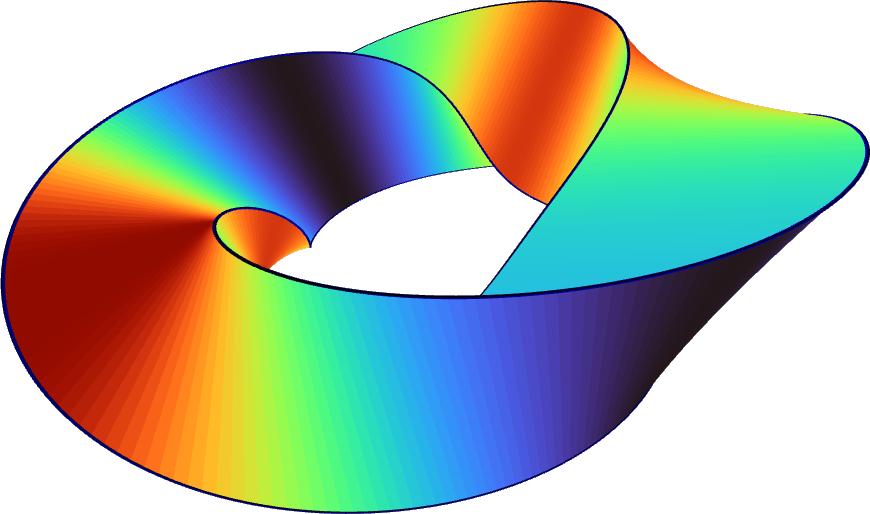
\includegraphics[width=.8\textwidth]{001_front_cover.png}}

% authors in alpha order
\author{Ronaldo A. Garcia \& Dan S. Reznik} 
\maketitle
%\frontmatter
\chapter*{Preface}
\textcolor{red}{to be written}
% A preface is written by the author and tells readers how and why the book came into being.
The stream of ideas and experiments in this book started with informal conversations in 2011 with Prof. Jair Koiller over açaí\footnote{A famed brazilian smoothie}, during warm weekend afternoons in Rio de Janeiro, Brazil.

Topics covered included the optics of light rays in an elliptic cavity. Soon this evolved to the closely-related mathematical topic of elliptic billiards, which gave way to budding simulation work (2011) followed by an 8-yr pause.




\textcolor{red}{material below needs to be rewritten}

geometry of elliptic billiard trajectories, following one author's recent work in control of heliostat fields for solar energy plants\footnote{Such fields are in fact a discretized/flattened focusing paraboloid, see \cite{sundrop2016,esolar2017}.}; see \cite{gross2020-solar} for a recent publication. An early, naïve experimental artifact was an animation of 3-periodics in the elliptic billiard along with the locus of their incenter; see  \cite{dsr_vid11incenter}. A natural choice given that each vertex is bisected by the ellipse normal. At the time we did not know this locus could be an ellipse, and indeed, how rare a find this is (we have conjecture that amongst the 5d space of possible ellipse pairs, only in the confocal pair -- a 1d subspace -- can the locus of the incenter be a conic). A twin animation was also produced depicting the self-intersected locus of the intouchpoints; see \cite{dsr_vid11e}.

Shortly thereafter \cite{olga14} produced a proof using methods of complex algebraic geometry.
%by complexification of the phenomenon. 
This was followed by an alternative    proof using techniques of real analytic   geometry given explicitly the equation of the locus; see \cite{garcia2019-incenter}. The loci centroids of Poncelet polygons was studied in \cite{schwartz2016-com}. In  \cite{garcia2019-incenter} the centroid locus was given explicitly.  Also \cite{corentin2021-circum} and \cite{garcia2018} proved that the locus of the circumcenter over billiard 3-periodics is also an ellipse.
 %\tableofcontents
%\mainmatter

\chapter{Introduction}
\label{chap:01-intro}

\begin{figure}
\centering
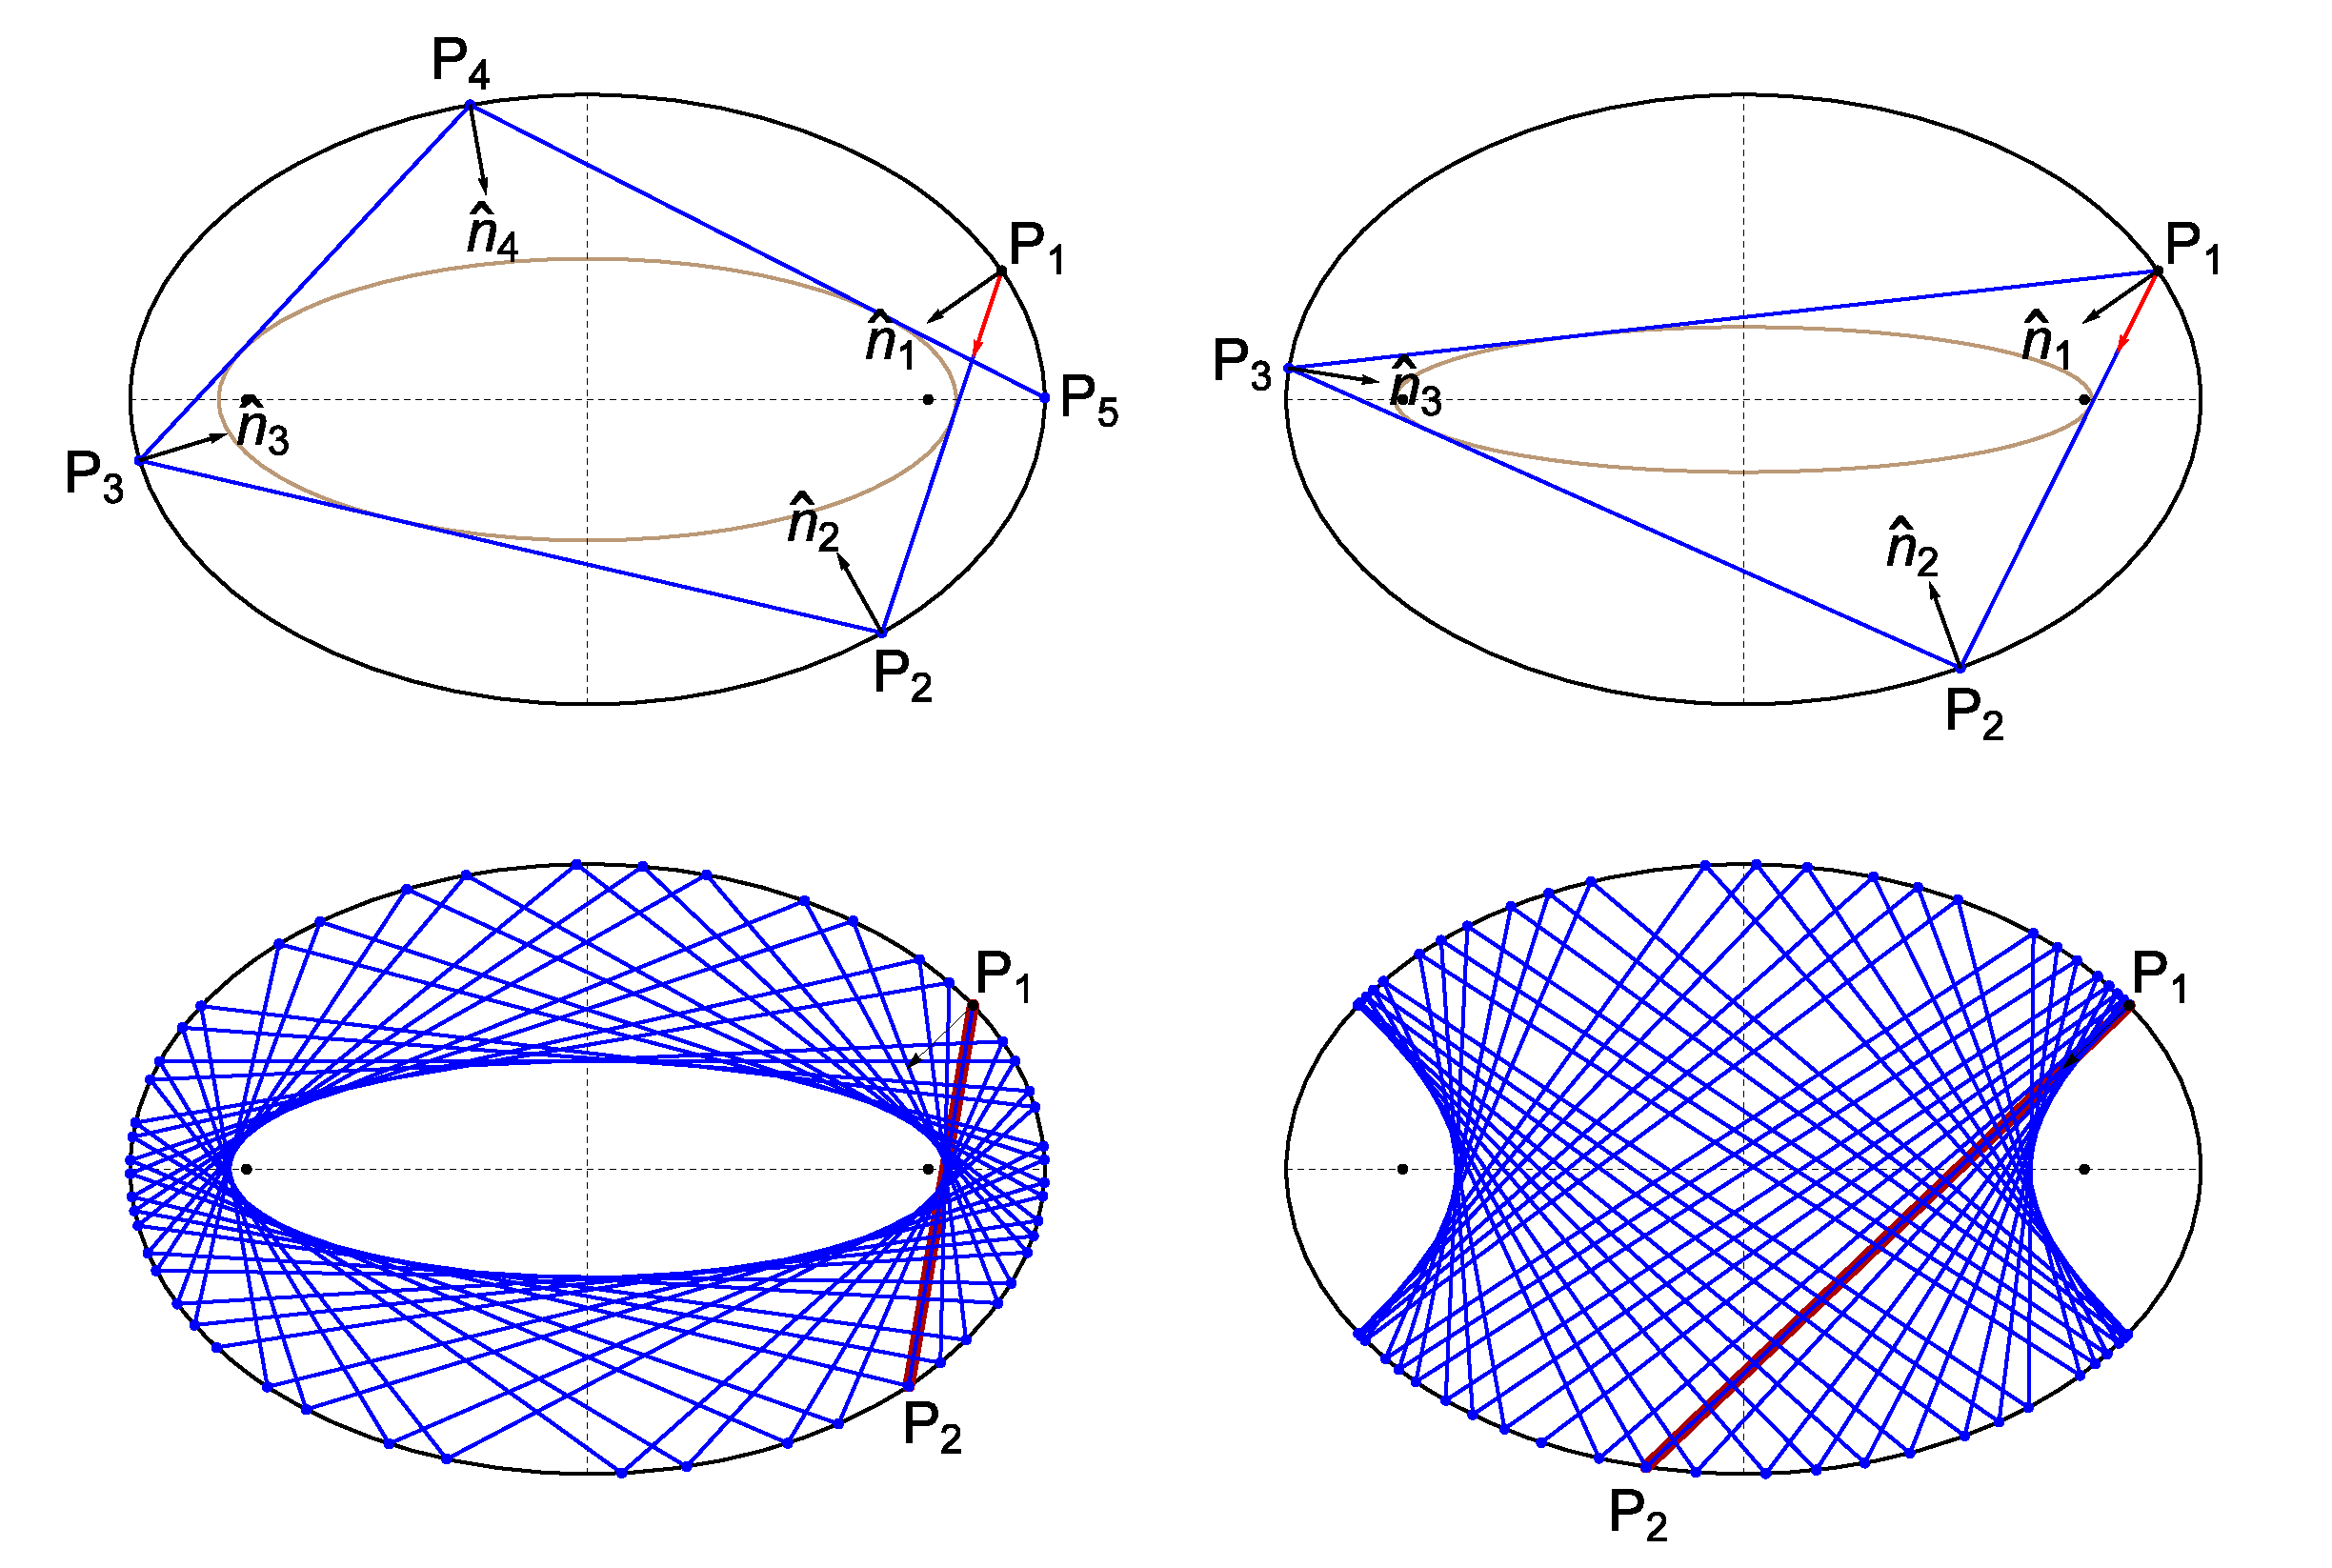
\includegraphics[width=\textwidth]{pics_01_010_billiard_trajectories.eps}
\caption{Trajectory regimes in the elliptic billiard. \textbf{Top left}: The first four segments of a trajectory departing at $P_1$ and moving toward $P_2$, bouncing at $P_i, i=2,3,4$. At each bounce the normal $\hat{n}_i$ bisects incoming and outgoing segments. Joachimsthal's integral \cite{sergei91} means all segments are tangent to a confocal {\em caustic} (brown). \textbf{Top right}: All 3-periodic orbits are tangent to a confocal caustic (brown). \textbf{Bottom}: The first 50 segments of a non-periodic trajectory starting at $P_1$ and directed toward $P_2$. Segments are tangent to a confocal ellipse (left) or hyperbola (right). The former (respectively, latter) occurs if $P_1P_2$ passes outside (respectively, between) the elliptic billiard's foci (black dots). Early \href{https://youtu.be/A7mPzrNJHkA}{Video 1}, \href{https://youtu.be/9zAr5-nm7mw}{Video 2}, \href{https://youtu.be/6yXA0dyWhFY}{Video 3}}
\label{fig:01-billiard-trajectories}
\end{figure}

\begin{figure}
\centering
\begin{subfigure}[t]{0.45\textwidth}
 \centering
 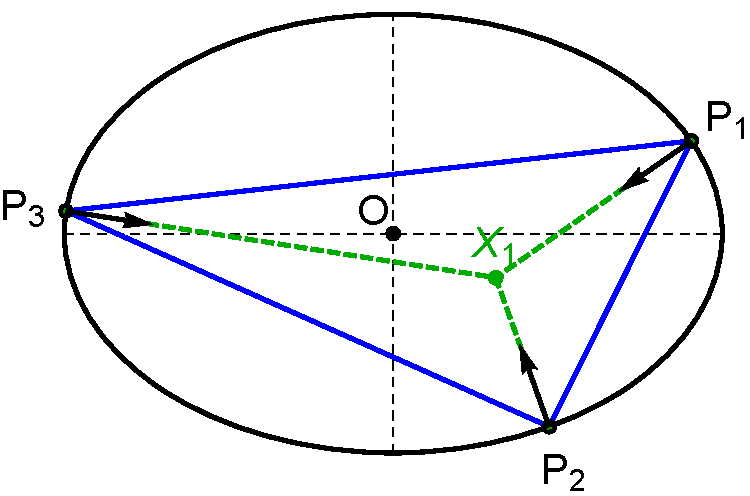
\includegraphics[width=\textwidth]{pics_01_030_single_orbit.pdf}
\end{subfigure}
\hfill
\begin{subfigure}[t]{0.45\textwidth}
 \centering
  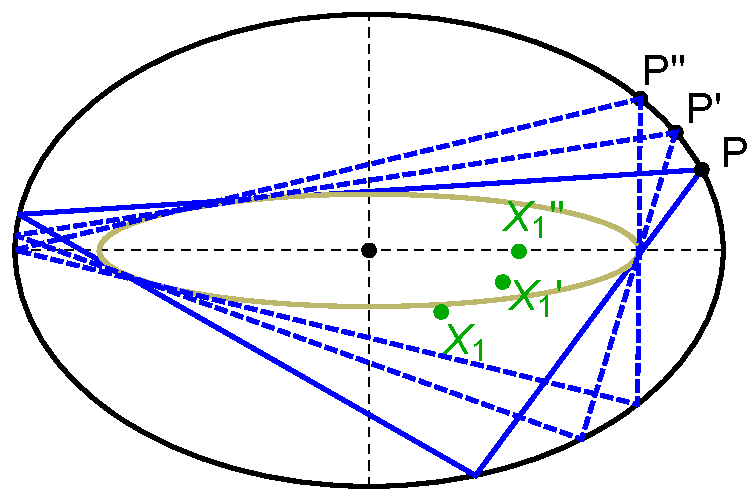
\includegraphics[width=\textwidth]{pics_01_040_three_orbits.pdf}
\end{subfigure}
     \caption{\textbf{Left:} An $N=3$ {\em orbit}. Its incenter $X_1$ is where angular bisectors (black arrows) concur. \textbf{Right}: Three billiard 3-periodics tangent to a confocal caustic (brown). Over positions $P,P',P''$ of a first vertex. Also shown are the corresponding incenters $X_1,X_1',X_1''$.  
\href{https://youtu.be/Y3q35DObfZU}{Video} }
\label{01-basic-n3}
\end{figure}


\begin{figure}
\centering
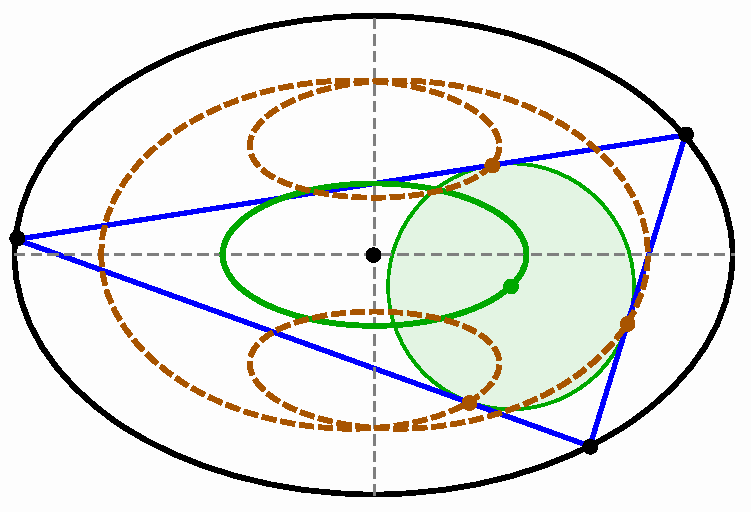
\includegraphics[width=.7\textwidth]{pics_01_020_intouch_locus.pdf}
\caption{An $N=3$ orbit (blue), its Incircle (transparent green), Incenter (green dot) and Intouch Points (brown dots). Over the $N=3$ family, the Incenter locus is a perfect ellipse (green), while the Intouchpoints produce a self-intersecting sextic (dashed brown).
% done
\href{https://youtu.be/9xU6T7hQMzs}{Video}, \href{https://bit.ly/3io8lgN}{Live}}
\label{fig:01-intouch-locus}
\end{figure}

\subsection*{Book Organization}

\begin{itemize}
    \item 
\end{itemize}




\input{chap_01/01_030_related}
\input{chap_01/01_040_structure}



\part{\torp{$N=3$}{N=3} Phenomena}

\chapter{Confocal Pair}
\label{chap:02-n3-confocal}
\section{Preliminaries}

Henceforth let {\em billiard 3-periodics} refer to the 1d family of Poncelet triangles interscribed between pair of confocal ellipses $\E$ and $\E_c$ given by:
\[ \E:\frac{x^2}{a^2}+\frac{y^2}{b^2}-1=0,\;\;\;\E_c:\frac{x^2}{a_c^2}+\frac{y^2}{b_c^2}-1=0\]
where $c^2=a^2-b^2=a_c^2-b_c^2$.

Billiard N-periodics classically conserve  perimeter $L$ and Joachimsthal's constant $J$. The latter one is equivalent to stating all trajectory segments are tangent to a confocal caustic, see \cite[Thm 4.4]{sergei91} and \cite{arnold2020-joachim}.
When $N=3$, we can derive these explicitly using the vertex parametrization given in \cref{eq:02-p2}.
 
\begin{proposition}
For billiard 3-periodics, the perimeter and Joachimsthal's constant are given by:

\begin{equation*}
J=\frac{\sqrt{2\delta-a^2-b^2}}{c^2},\;\;\;L=2(\delta+a^2+b^2)J
\label{eqn:n3-L-J}
\end{equation*}
where $\delta=\sqrt{a^4-a^2b^2+b^4}$.
\end{proposition}

\begin{proof} We compute the values considering  an isosceles 3-periodic with $P_1=[a,0]$, and

% {\small  
% \begin{equation}\label{eq:isosceles_3orbit}
%  \;  P_2   =\left[-\frac {{a}^{2}\sqrt {2\,\delta-{a}^{2}-{b}^{2}}}{c^2},   
%	\frac { \left(\delta  -{a}^{2}\right) b}{c^2}\right],\;\;
%	    P_3= \left[{-\frac {{a}^{2}\sqrt {2\,\delta-{a}^{2}-{b}^{2} }}{c^2}},
%	{\frac { \left(  {a}^{2}-\delta \right) %b}{c^2}}\right]
%\end{equation}
 %}%
 {\small 
 \begin{equation} \label{eq:orbita3-isosceles}
 P_2=\left[   {\frac {a \left(  {b}^{2}-\delta \right) }{   a^2-b^2 
 			  }},{\frac {{b}^{2}\sqrt {2 \delta -{a}^{2}-{b}^{2}\,
 				}}{{a}^{2}-{b}^{2}}} 
 	\right], \;\; P_3=\left[  {\frac {a \left(  {b}^{2}-\delta \right) }{   a^2-b^2   
 	}},-{\frac {{b}^{2}\sqrt {2\delta-{a}^{2}-{b}^{2} 
 				}}{{a}^{2}-{b}^{2}}} 
 	\right]
 	\end{equation}
 	}
 	We have that
 	\[L=|P_2-P_3|+2|P_1-P_2|,\;\;
 	 J=\langle \frac{P_1-P_3}{|P_1-P_3|},[\frac{1}{a},0]\rangle\]
 	 Straightforward calculations using the vertex parametrization in \cref{eq:02-p2}, leads to the stated result.
%\textcolor{red}{ronaldo: CAS+parametrization}
\end{proof}

Henceforth the oft-ocurring quantity $\delta$ will be referred to as the Darboux constant. An interesting geometric interpretation for it appears in \cref{prop:02-delta}.

%\noindent Note: the use of $J$ in this chapter refers to its value for the $N=3$ case.

\section{Caustic semi-axes}

The Cayley condition for a concentric, axis parallel (CAP) pair of ellipses to admit a 3-periodic family is given by:

\begin{equation} \frac{a_c}{a}+\frac{b_c}{b}=1
\label{eqn:n3-cayley}
\end{equation}

In turn, this constrains the semi-axes of the confocal caustic.

\begin{proposition}
The semi-axes $a_c,b_c$ of the confocal caustic are given by:
\begin{align*}
a_c=&\frac{a\left(\delta-{b}^{2}\right)}{c^2},\;\;\;\;
b_c=\frac{b\left({a}^{2}-\delta\right)}{c^2}\cdot
\end{align*}
\label{prop:02-n3-caustic}
\end{proposition}

When $a=b$, we have that $a_c=b_c=a/2$.

\begin{proposition}
The semi-axes $a$ and $b$ of the ellipse in terms of the semi-axes $a_c$ and $b_c$ of the confocal ellipse are given by:
\begin{align*}
a&= -\frac{1}{2} \sqrt{w_1} + \frac{1}{2} \sqrt{ w_2 -\frac{ 2 a_c^3 - 4 c^2a_c}{\sqrt{w_1}} } +\frac{a_c}{2},\;\; b=\sqrt{a^2-c^2}\\
w_1&=a_c^2-(4 c a_c b_c)^{\frac{2}{3}},\;\; w_2=2 a_c^2+ (4 c a_c b_c)^{\frac{2}{3}}
\end{align*}
The implicit equation that defines $a$ above is the quartic  given by
\[c^2( a_c^2   - 2   a_c   a )+ a^2(2a_c a  - a^2)=0\]
\label{prop:02-caustic-to-billiard}
\end{proposition}

\section{Incenter and excenter loci}
\label{sec:02-inc-exc-loci}

\begin{figure}
    \centering
    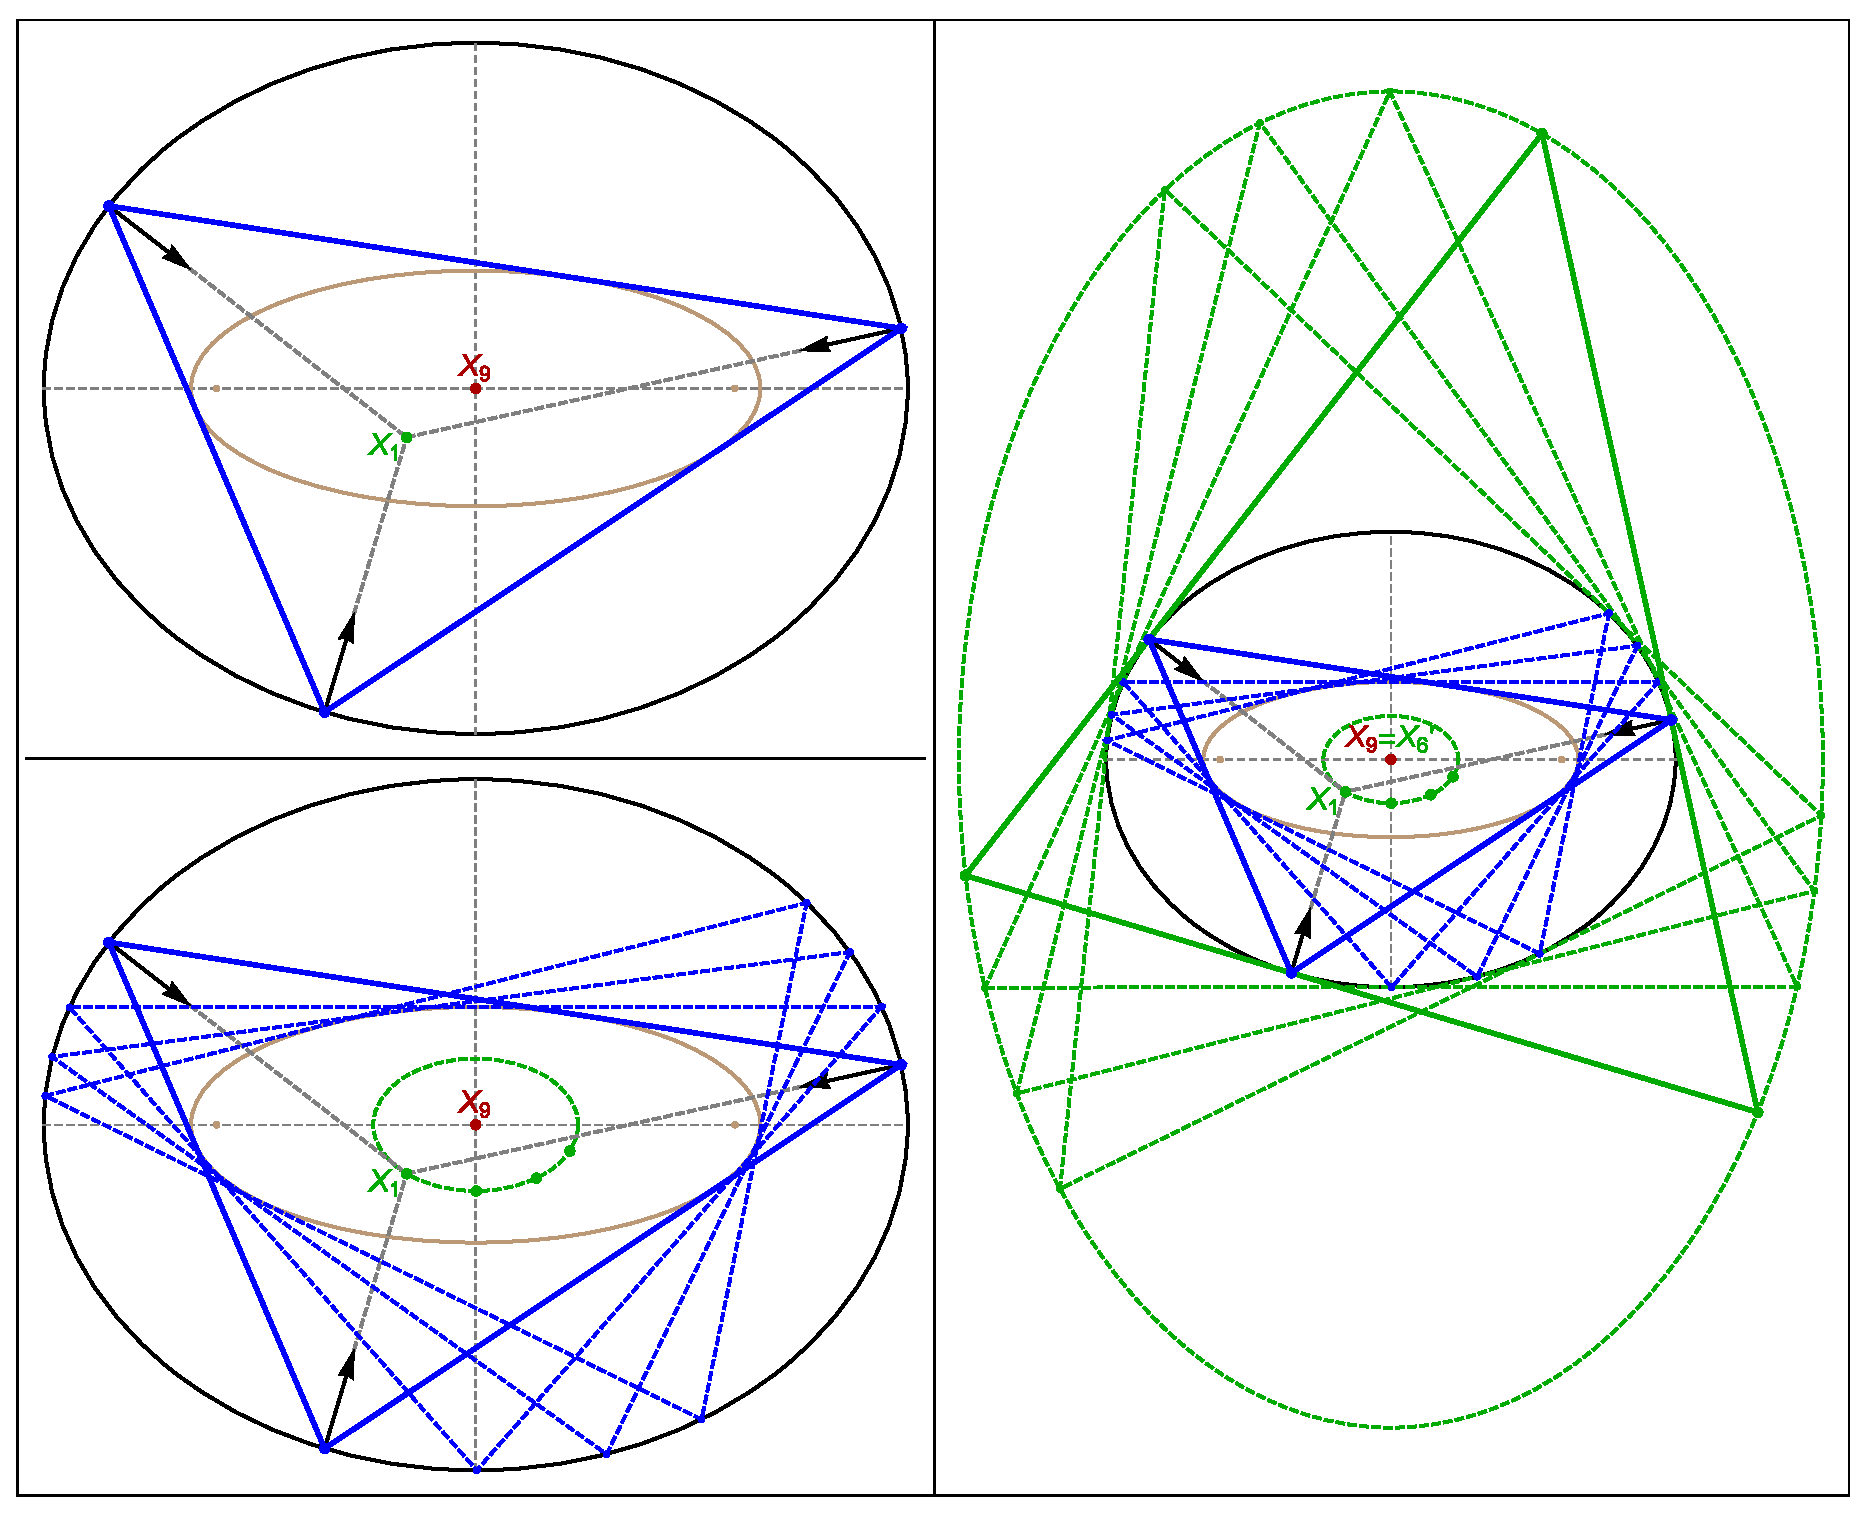
\includegraphics[width=\textwidth]{pics_02_010_billiard_grid}
    \caption{\textbf{Top Left:} An elliptic billiard 3-periodic (solid blue) is shown inscribed in an outer ellipse (black) and a confocal caustic (brown). Graves' theorem implies its internal angles will be bisected by ellipse normals (black arrows). Also shown is the incenter $X_1$ defined as the intersection of said bisectors. \textbf{Bottom Left:} Poncelet's porism implies a 1d family of such triangles exists. Some samples are shown (dashed blue). A classic invariant is  perimeter. The Mittenpunkt $X_9$ remains stationary at the center. The incenter $X_1$ sweeps an ellipse (dashed green). \textbf{Right:} The excentral triangle (solid green) has sides perpendicular to the bisectors. Over billiard 3-periodics, the excentral is of variable perimeter. Its vertices (known as the ``excenters'') also sweep an ellipse (dashed green) whose aspect ratio is the reciprocal of that of the incenter locus. The Symmedian point $X_6'$ of the excentral triangle coincides with $X_9$ of the reference and is therefore stationary. \href{https://bit.ly/3gWl3CI}{Live}}
    \label{fig:billiard-grid}
\end{figure}

An intriguing phenomenon is that over billiard 3-periodics, the locus of both incenter and the excenters are ellipses, as was initially detected experimentally (see an early \href{https://youtu.be/BBsyM7RnswA}{Video}). This was proved by \cite{olga14} and \cite{garcia2019-incenter}. Indeed, we haven't yet found another Poncelet pair where this is the case, see \cref{conj:07-incenter-excenter-loci}.

Referring to \cref{fig:billiard-grid}:

\begin{theorem}
Over billiard 3-periodics, the locus of the incenter $X_1$ and excenter are ellipses $\E_1$ and $\E_e$ concentric and axis-parallel with the confocal pair whose axes $(a_1,b_1)$ and $(a_e,b_e)$ are given by:
\begin{align*}
a_1 =& \frac{\delta-b^2 }{a},\;\;\;b_1=\frac{a^2-\delta}{b}\\ 
a_e= &\frac{{b}^{2}+\delta}{a},\;\;\;b_e=\frac{{a}^{2}+\delta}{b}
\end{align*}
Furthermore, $\E_1$ and $\E_e$ have reciprocal aspect ratios, i.e., $a_1/b_1=b_e/a_e$.
\label{thm:02-incenter-excenter}
\end{theorem}

\begin{proof}
It follows from the vertex parametrization in \cref{eq:02-p2} and the definition of incenter and excenters. We have that
\[X_1=\frac{s_1 P_1+s_2P_2+s_3P_3}{s_1+s_2+s_3}=
\frac{1}{L}(s_1P_1+s_2P_2+s_3P_3)\]
where $s_1=|P_2-P_3|$, $s_2=|P_1-P_3|$ and $s_3=|P_1-P_2|$.
A careful symbolic analysis shows that $\mathcal{E}_1(X_1)=0$. A similar analysis considering the excenters shows that the locus of the three points is the ellipse $\mathcal{E}_e$ stated.
\end{proof}

\noindent A more general treatment to the above is given in \cref{chap:07-n3-loci}.

\begin{corollary}
The pair $\{\mathcal{E},\mathcal{E}_e\}$ is Ponceletian.
\label{cor:02-excentral-billiard-poncelet}
\end{corollary}

\begin{proof}
Direct from Cayley condition
\[\frac{a}{a_e}+\frac{b}{b_e}=\frac{a^2}{b^2+\delta}+\frac{b^2}{a^2+\delta}= 1\]

\end{proof}

\section{A stationary point}
\label{sec:02-stationary}

The Mittenpunkt $X_9$ is a triangle center where lines from each excenter thru the side midpoint meet. Referring to \cref{fig:02-x9}:
\begin{theorem}
Over the family of 3-periodics in the elliptic billiard, $X_9$ is stationary at the common center.
\end{theorem}

An elegant syntethic proof was kindly contributed by \cite{olga19_mitten}:

\begin{proof}
Let $\E$ be the outer ellipse in the confocal pair, $O$. By definition, the Mittenpunkt $X_9$ is where lines from the excenters $E_i$ through the side midpoints $M_i$ concur. Notice each side is an ellipse chord between tangents to $\E$ seen from the $E_i$ (this is because in the confocal pair the excentral triangle is tangent to $\E$). Consider the image of lines $E_i M_i$ under an affine transform which sends $\E$ to a circle $\Cm'$, let $O'$ be its center. The transformed lines will pass through the midpoints of chords of $\Cm'$ between tangents seen from $E_i'$ (the affine image of $E_i$). By circular symmetry, such lines must also pass through $O'$, and therefore remain stationary. But $O'$ is the affine image of $O$, so the result follows.
\end{proof}

\begin{figure}
     \centering
    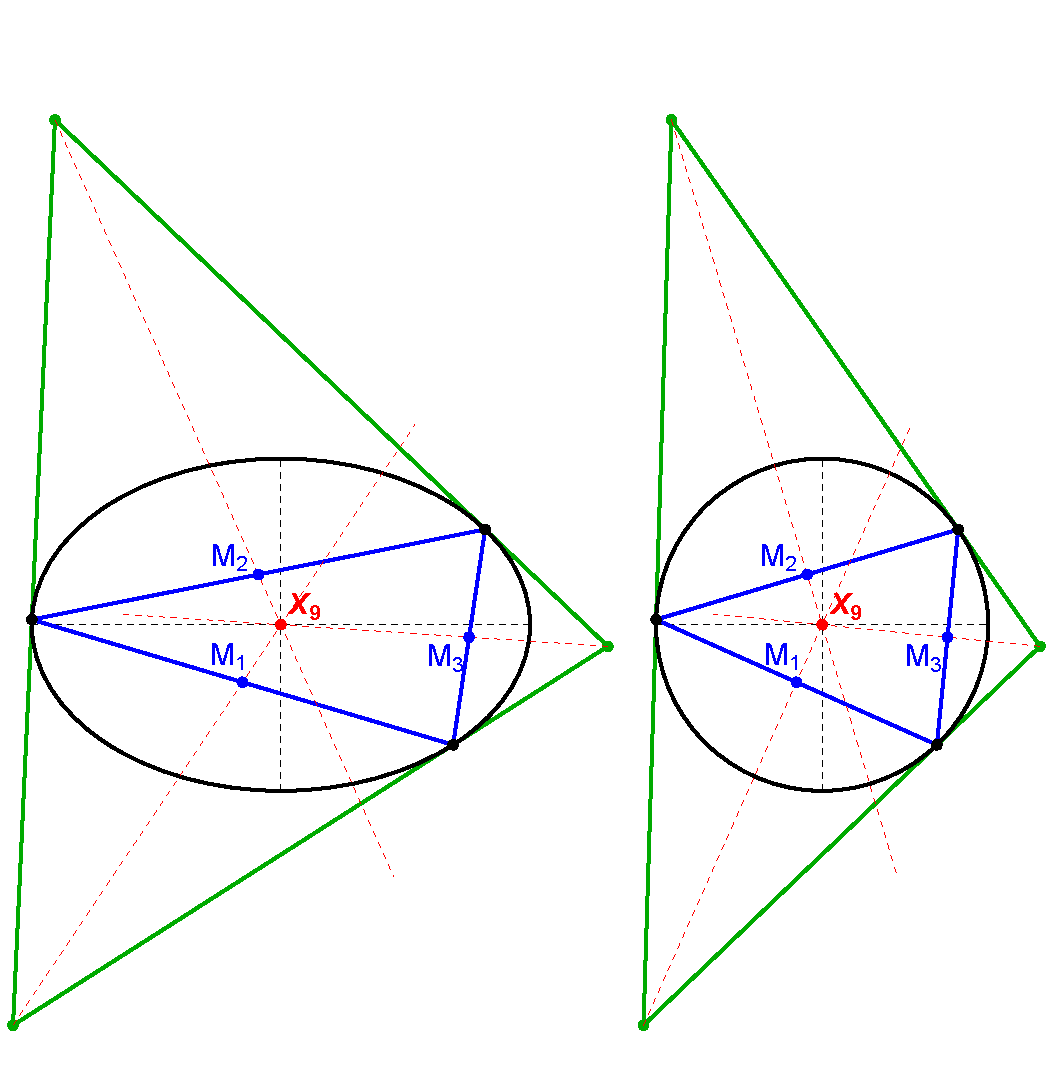
\includegraphics[width=\linewidth]{pics_02_020_mitten_proof.pdf}
     \caption{\textbf{Left}: 3-periodic billiard triangle (blue), its excentral triangle (green). The Mittenpunkt $X_9$ is the point of concurrence of lines drawn from the excenters through sides' midpoints $M_i$. \textbf{Right}: the affine image which sends the billiard to a circle. Lines from imaged excenters through sides' midpoints must pass through the origin. Since the latter is stationary, so must be its pre-image $X_9$, which is stationary at the billiard center.  % done
     \href{https://youtu.be/tMrBqfRBYik}{Video}}
     \label{fig:02-x9} 
\end{figure}

\section{Conserved Quantities}

Given a triangle, let $r$ and $R$ denote the radius of its incircle and circumcircle, known as the {\em inradius} and {\em circumradius}, respectively. Over billiard 3-periodics, note these two radii are variable. Referring to \cref{fig:radii}:

\begin{theorem}
$r/R$ is invariant over billiard 3-periodics and given by:
\begin{equation*}
\label{eqn:rovR}
\frac{r}{R}=\frac{2 (\delta-b^2)(a^2-\delta)}{c^4}.
\end{equation*}
\label{thm:02-confocal-rovR}
\end{theorem}

\begin{proof}
The following relation, found in \cite{johnson1960}, holds for any triangle:

\begin{equation*}
 r R=\frac{s_1s_2s_3}{2 L}, 
\end{equation*}

\noindent where $L=s_1+s_2+s_3$ is the perimeter, constant over billiard 3-periodics. Therefore:

\begin{equation}
\frac{r}{R}=\frac{1}{2L} \frac{s_1s_2s_3}{R^2}\cdot
\label{eqn:rovR-cas}
\end{equation}

Next, let $P_1=(a,0)$ be a vertex of an isosceles 3-periodic. Obtain a candidate expression for $r/R$. This yields \eqref{eqn:rovR} exactly. Using the vertex parametrization in \cref{eq:02-p2}, derive an expression for the square of the right-hand side of \eqref{eqn:rovR-cas} as a function of $x_1$ and subtract from it the square of \eqref{eqn:rovR}. In  \cite{garcia2020-new-properties}
it is shown $\left(s_1s_2s_3/R^2\right)^2$ is rational on $x_1$. For simplification, use $R=s_1 s_2 s_3/(4A)$, where $A$ is the triangle area. With a CAS, show said difference is identically zero for all $x_1\in(-a,a)$.
\end{proof}


\begin{figure}
    \centering
    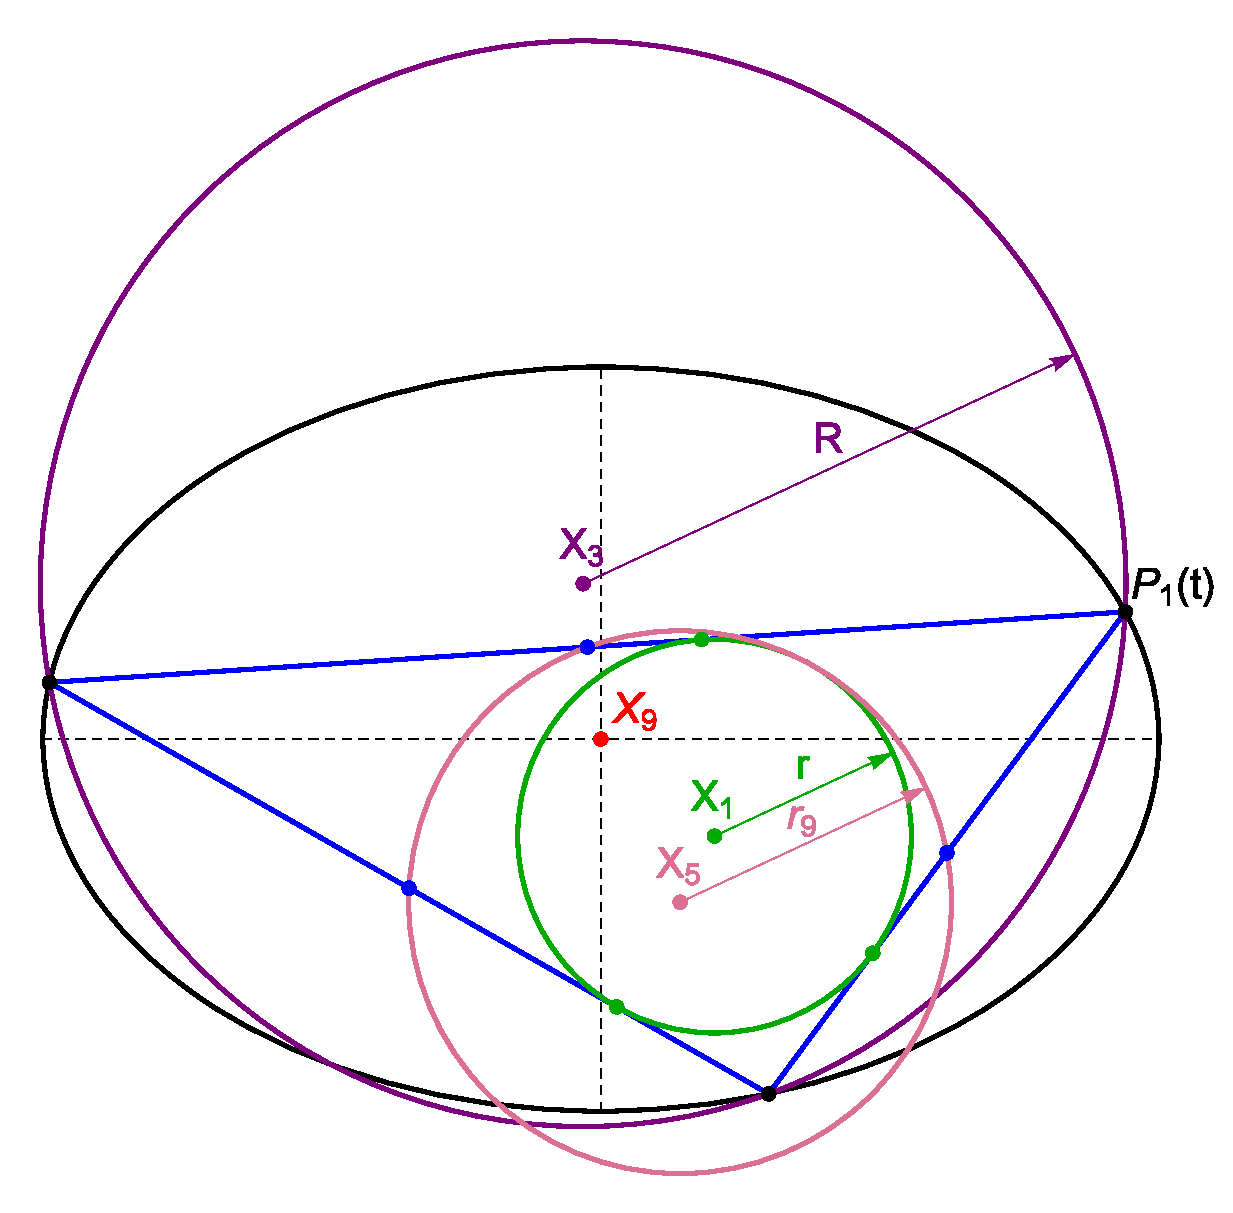
\includegraphics[width=\textwidth]{pics_02_030_radii}
    \caption{The incircle (green), circumcircle (purple), and 9-point (Euler's) circle (pink) of a billiard triangle (blue). These are centered on $X_1$, $X_3$, and $X_5$, respectively. Their radii are the inradius $r$, circumradius $R$, and 9-point circle radius $r_9=2R$. Over the family, the ratio $r/R$ is invariant. In turn this implies an invariant sum of cosines. \href{https://bit.ly/337hvpf}{Live}}
    \label{fig:radii}
\end{figure}

Let $\theta_i$, $r$, $R$, and $A$ denote the ith internal angle, inradius, circumradius, and area of a reference triangle. Primed quantities refer to the excentral triangle. The relations below, appearing in  \cite{johnson1960},  hold for any triangle:

\begin{align}
\sum_{i=1}^{3}{\cos\theta_i}&=1+\frac{r}{R} \label{eqn:02-sum-cos} \\
\prod_{i=1}^{3}{\cos\theta_i'}&=\frac{r}{4R} \label{eqn:02-exc-prod-cos} \\
\frac{A}{A'}&=\frac{r}{2R} \label{eqn:02-area-ratio}
\end{align}

\begin{corollary}
Over billiard 3-periodics, also invariant are the sum of 3-periodic cosines, the product of excentral cosines, and the ratio of excentral-to-3-periodic areas.
\label{cor:02-rOvR}
\end{corollary}

Direct calculations yields an expression for the invariant sum of cosines in terms of elliptic billiard constants $J$ and $L$.

\begin{corollary}
$\sum_{i=1}^{3}{\cos\theta_i}=J L - 3$
\end{corollary}

Indeed in \cite{akopyan2020-invariants} it is shown that for all $N$ the sum of cosines is invariant and equal to $J L-N$.

Let $P_i$ be a billiard 3-periodic vertex and $d_{j,i}=|P_i-f_j|$ its distance to billiard focus $f_j$. 

\begin{proposition}
 Over billiard 3-periodics, the following sum is invariant:
\[  \sum\frac{1}{d_{1,i}}=\sum\frac{1}{d_{2,i}}=\frac {{a}^{2}+{b}^{2}+\delta}{a{b}^{
2}}
\]
\label{prop:02-confocal-inv-spokes}
\end{proposition}

\begin{proof}
Direct computation with CAS using vertex parametrization given in \cref{sec:02-vertex-para}.
\end{proof}

Let $P=(x,y)$ be a point on an ellipse with semi-axes $a,b$. In \cite[Ellipse]{mw}, the curvature at $P$ is expressed both in terms of its coordinates and the distances $d_1,d_2$ to the foci as follows:

\begin{equation}
\kappa = \frac{1}{a^2 b^2} \left(\frac{x^2}{a^4}+\frac{y^2}{b^4}\right)^{-3/2} = \frac{a b}{(d_1 d_2)^{3/2}}
\label{eqn:02=curv}
\end{equation}

Let $\kappa_i$ denote the billiard ellipse curvature at vertex $P_i$ of a Poncelet 3-periodic. From the above and \cref{prop:02-confocal-inv-spokes} obtain:

\begin{corollary}
Over billiard 3-periodics, the following quantity is conserved:
\[ \sum_{i=1}^3{\kappa_i^\frac{2}{3}} =\frac{ a^2 + b^2 + \delta}{ (ab)^{\frac{4}{3}} }\]
\label{prop:02-confocal-curv-sum}
\end{corollary}

\section{An interpretation for \torp{$\delta$}{delta}}

The Darboux constant $\delta$ appearing above has a curious geometric interpretation. Recall the power of a point $Q$ with respect to a circle $\Cm=(C_0,R_0)$ is given by $|Q-C_0|^2-R_0^2$, see \cite[Circle Power]{mw}. Let $\Cm$ denote the (moving) circumcircle of billiard 3-periodic, and $O=X_9$ the billiard center.

\begin{proposition}
The power of $O$ with respect to $\Cm$ is constant and equal to $-\delta$.
\label{prop:02-delta}
\end{proposition}

\begin{proof}
Consider an isosceles billiard 3-periodic given by \cref{eq:orbita3-isosceles}.
	Its circumcircle will be centered at $C_0=[ {\frac { {b}^{2}-\delta}{2b}},0]$ with circumradius $R_0=\frac {{b}^{2}+\delta}{2b}.$
	Therefore, the power of the center of the ellipse with respect to the circumcircle is given by  
	$$|OC_0|^2-R_0^2=\left(\frac { {b}^{2}-\delta}{2b}\right)^2 - \left(\frac {{b}^{2}+\delta}{2b}\right)^2=-\delta.$$
	
	The stated invariance is confirmed with a CAS using the vertex parametrization in \cref{eq:02-p2}.  
%	\textcolor{red}{localizar depois}
\end{proof}




\section{Confocal Vertex Parametrization}

We describe two parametrizations for billiard 3-periodic vertices: (i) standard and (ii) Jacobi.

\subsection{Standard}
\label{sec:02-confocal-standard-param}

We call ``standard'' parametrization that where a first vertex $P_1(t)$ of the billiard 3-periodic is parametrized as $P_1(t)=[x_1,y_1]=[a\cos{t},b\sin{t}]$.

As derived in \cite{garcia2019-incenter}, $P_2=(x_2,y_2)/q_2$ and $P_3=(x_3,y_3)/q_3$ where:

 \begin{equation}
 \label{eq:02-p2}
 \aligned 
x_{2}=&-{b}^{4} \left(  \left(   a^2+{b}^{2}\right)\cos^{2}\alpha   -{a}^{2}  \right) x_1^{3}-2{a}^{6} \,\cos  \alpha  \sin   \alpha  \, y_1^{3}\\
&+{a}^{4} \left(  ({a
}^{2}-3\, {b}^{2}) \cos^{2} \alpha  +{b}^{2}
 \right) {x_1}\,y_1^{2}-2\,{a}^{4}{b}^{2} \cos \alpha  \,\sin  \alpha    x_1^{2}{y_1},
\\
y_{2}=& 2{b}^{6} \,\cos \alpha\sin \alpha\,   x_1^{3}-{
a}^{4}  \left(  \left(   a^2+{b}^{2}\right)\cos^{2}  \alpha  -{b}^{2}  \right)  y_1^{3}\\
&+  2\,{a}^{2} {b}^{4}\cos \alpha \sin
  \alpha \; {x_1} y_1^{2} +{b}^{4}\left(  ({b
 }^{2}-3\, {a}^{2}) \cos^{2} \alpha  +{a}^{2}
  \right) x_1^{2}{y_1}
\\
q_2=&{b}^{4} \left( a^2-(a^2-b^2)\cos^2  \alpha   \right)
x_1^{2}+{a}^{4} \left(  {b}^{2}+(a^2-b^2)\cos^2 \alpha  
 \right) y_1^{2}\\
 & - 2\, {a}^{2}{b}^{2} \left({a}^{2} -{b}^{2} \right)\cos \alpha\sin \alpha \; {x_1}\,{
y_1}.
\endaligned
%
\end{equation}

 \begin{equation} \label{eq:02-p3} \aligned 
x_{3}\; =& \; {b}^{4} \left( {a}^{2}- \left( {b}^{2}+{a}^{2} \right) 
 \cos^{2}\alpha\right)   x_1^{3}+2\, {a}^{6} 
 \cos \alpha\,\sin \alpha\, y_1^{3}\\
 &+{a}^{4} \left( 
  \cos^{2}  \alpha  \left( {a}^{2}-3\,{b}^{2}
 \right) +{b}^{2} \right) { x_1}\, y_1^{2}+2\,{a}^{4}{b}^{2} \cos  \alpha\sin \alpha\,   x_1^{2}{ y_1}
\\
y_{3} \;=&\; -2\, {b}^{6} \cos \alpha\sin \alpha\, x_1^{3}+
{a}^{4} \left( {b}^{2}- \left( {b}^{2}+{a}^{2} \right)   \cos^{2}  \alpha  \right)\,  y_1^{3}\\
& -2\,{a}^{2}  {b}^{4}\cos
 \alpha  \sin \alpha\,  x_1 y_1^{2}+
{b}^{4} \left( {a}^{2}+ \left( {b}^{2}-3\,{a}^{2} \right)  \left( \cos
 \alpha  \right) ^{2} \right) {{ x_1}}^{2}{ y_1},
\\
q_3 \;=& \; {b}^{4} \left( {a}^{2}- \left(a^2 -{b}^{2}  \right)   \cos^{2} \alpha   \right) x_1^{2}+{a}^{4} \left( {b}^{2}+ \left( a^2-{b}^{2}  \right)  \cos^{2} \alpha  \right)  y_1^{2}\\
&+2\,{a}^{2}{b}^{
2} \left( {a}^{2}-{b}^{2} \right) \cos \alpha \sin \alpha\, { x_1}\,{ y_1}.
\endaligned
%
\end{equation}
where:
\[\cos \alpha={\frac {a^2 b  \, \sqrt {-{a}^{2}-{b}^{2}+2\,\sqrt {{a}^{4}-{b}^{2}{c}^{2}}}}{{c}^{2}\sqrt {{a}^{4}-{c}^{2} x_1^{2}}}}=
\frac{  a^2 b^2 \, \sqrt {2\delta-{a}^{2}-{b}^{2}}} {c^2\sqrt{ a^4y_1^2 + b^4x_1^2}  } \]

Note that in \cref{sec:03-cap-vtx-param} we generalize the above to any concentric, axis-parallel pair.

\subsection{Jacobi's Universal Measure}
\label{sec:02-confocal-jacobi-param}

Under the standard parametrization, we can obtain the ``position'' $t$ of $P=[x,y]$ on an ellipse:

\[ t=\tan^{-1}{\frac{a y}{b x}}. \]

As shown in \cref{fig:02-jacobi-param}(top), when a first vertex $P_1(t)$ in the billiard 3-periodic is parametrized in the standard way, though its position is linear on the $t$ parameter, it will drive motions of the other two vertices $P_2(t)$ and $P_3(t)$ which are both distinct and non-linear. 

Fortunately, a uniform parametrization exists, which goes back to Jacobi, for all Poncelet families, based on the so-called ``universal measure'', which linearizes the Poncelet map, see \cite{koiller2021-spatial}. Specifically, vertices are obtained at fixed multiples of a constant $\Delta{u}$ in the argument of certain Jacobi elliptic functions. This parametrization, adapted to the elliptic billiard case, appears in \cite{stachel2021-billiards,stachel2021-billiards-param} and is reproduced below. First let's recall a few useful definitions. 

The  notation adopted below is as \cite{armitage-2006}. 

\begin{definition}
The incomplete elliptic integral of the first kind $K(\varphi,k)$ is given by:
\begin{equation}
K(\varphi,k)=\int_0^{\varphi}\frac{d\theta}{\sqrt{1-k^2 \sin^2\theta}}
\label{eqn:02-ellipticK}
\end{equation}
%\end{definition}

%\begin{definition}
The complete elliptic integral of the first kind $K(k)$ is simply $K(\pi/2,k)$.
\end{definition}

\begin{definition}
The elliptic sine $\text{sn}$, cosine $\text{cn}$, and delta-amplitude $\text{dn}$ are given by:
\begin{align*}
\text{sn}(u,k)&=\sin\varphi\\
\text{cn}(u,k)&=\cos\varphi\\
\text{dn}(u,k)&=\sqrt{1- k^2\sin^2\varphi}\\
\end{align*}
where $\varphi=\text{am}(u,k)$ is known as the amplitude, i.e., the upper-limit in the integral in \cref{eqn:02-ellipticK} such that $K(\varphi,k)=u$.
\end{definition}
A review of these functions appears in \cref{app:appD-jacobi-functions}.

\begin{remark}
Note to the reader: Mathematica (resp. Maple) expects $m=k^2$ (resp. $k$) as the second parameter to elliptic functions.

With this terminology the  Jacobi elliptic functions are defined    as follows:
\begin{align*}
K(\varphi,m)&=\int_0^{\varphi} \frac{dy}{\sqrt{1-m\sin^2y}}=u,\;\; \varphi=\text{am}(u,m)\\
%K(\varphi,k)=u\\ %
\sn(u,m)&=\sin\varphi,\; \cn(u,m)=\cos\varphi,\; dn(u,m)=\sqrt{1-m\sin^2\varphi}, \end{align*}

%As a note the reader, Maple accepts $k$ while Mathematica requires $m=k^2$ as the argument to elliptic functions.

%For example, in Maple we have: \[\sn(2,0.4)=\texttt{JacobiSN(2,.4)}=0.94569756\ldots\]
%and in Mathematica:

%\[ \sn(2,0.16)=\texttt{JacobiSN[2,.16]}=0.945698 \ldots \]
%and
%\[ \texttt{JacobiSN[2,.4]}=0.985090\ldots \]
\end{remark}

\begin{theorem}
A billiard orbit $P_i$ $(i=1,\ldots, N) $ of period $N$  with turning number $\tau$, where $\mathrm{gcd}(N,\tau) =1$,  is parametrized on $u$ with period $4K$ where:


\[ 
P_i=
%=\left[a\; \Jsn \left(u+\frac{4n\tau K}{N}, \frac{c}{a}\right), b\; \Jcn \left(u+\frac{4n\tau K}{N}, \frac{c}{a}\right)\right]\\
\left[-a\,\sn  \left(u+ i \Delta{u},  {m} \right) , b\,\cn  \left(u + i \Delta{u}, { m} \right)\right]
\]

where,
\[ m=k^2=\frac{a_c^2-b_c^2}{a_c^2},\;\;\Delta{u}=\frac{4\tau K}{N}\]
\[a= \sqrt{b^2+ a_c^2-b_c^2}, \;\; b=\frac{b_c}{\cn(\frac{\Delta{u}}{2}, m)}\]
\end{theorem}
\begin{proof} See \cite{stachel2021-billiards}.\end{proof}

A basic fact to obtain this parametrization is the following.

\begin{figure}
    \centering
    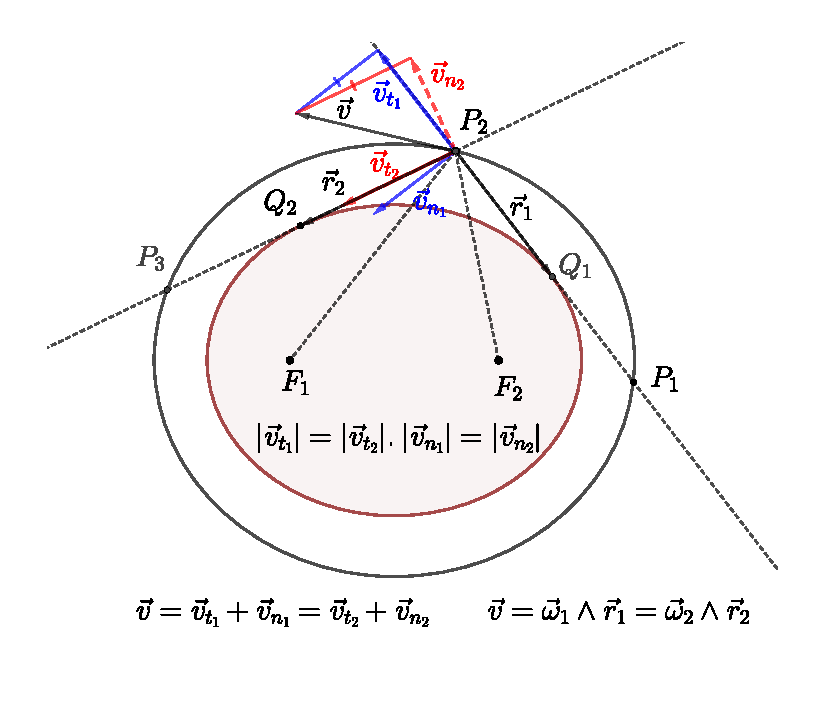
\includegraphics[width=\textwidth]{pics_02_040_param_jacobi.pdf}
    \caption{ Angular velocity $\vec v=\vec \omega\wedge \vec r$. } 
    \end{figure}
Referring to \cref{fig:02-velocidade-angular}:

\begin{proposition} 
Consider   segment of orbits $P_1P_2$ and $P_2P_3$  and contact points $Q_1$ and $Q_2$ with the caustic in an elliptic billiard. Let $\vec v$ the vector velocity of $P_2(t)$. Let $\vec r_1=Q_1-P_2$ and $\vec r_2=Q_2-P_2$. Then
\[ |\vec \omega_1|\;|\vec r_1|=|\vec \omega_2|\; |\vec r_2|\]
where $\vec v=\vec\omega_1\wedge r_1= \vec\omega_2\wedge \vec r_2$.

\label{fig:02-velocidade-angular}
\end{proposition}

\begin{proof} Let $\vec v=P_2'(t)$. From Graves's theorem, $|\vec r_1|+|\vec r_2|-\text{arc}(Q_1,Q_2)=\text{cte}$,  and therefore it follows that in decomposition of $\vec v=\vec v_{t_1}+\vec v_{n_1}=\vec v_{t_2}+\vec v_{n_2}$ we have that $|\vec v_{t_1}|=|\vec v_{t_2}|$ and  $|\vec v_{n_1}|=|\vec v_{n_2}|$. The result follows from the   definition of angular velocity. More details see \cite{stachel2021-billiards-param}.
\end{proof}
 
\textcolor{red}{ronaldo}
 
Since in this chapter we are considering billiard 3-periodics, so above $N=3$, and $\tau=1$. As shown in \cref{fig:02-jacobi-param}, under the Jacobi parametrization each of the 3 vertices of billiard 3-periodics follows the exact same curve, albeit with a 120-degree phase.

Recall the sum of cosines is constant for billiard 3-periodics. \cref{fig:02-jacobi-cos-param} shows how individual cosines follow either (i) 3-distinct curves, or (ii) the same exact curve (at different phases) if the parametrization is standard or Jacobi, respectively.

\begin{figure}
    \centering
    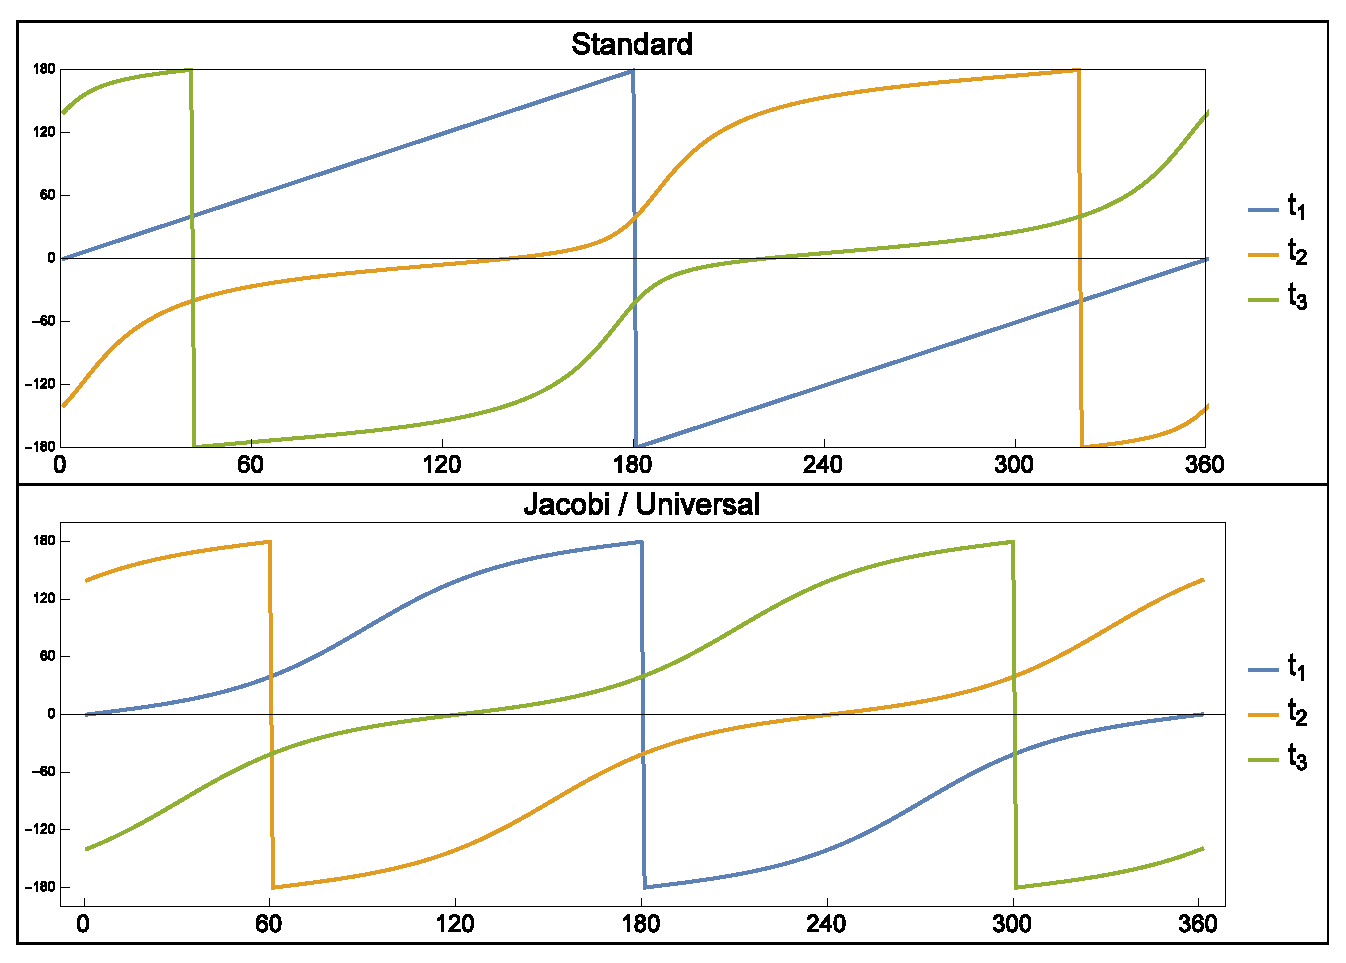
\includegraphics[width=\textwidth]{pics_02_050_parametrizations}
    \caption{The ``position'' $\theta_i$ (vertical axis) of a point on an ellipse with semi-axes $a,b$ vs the billiard 3-periodic parameter (horizontal axis). \textbf{Top:} vertex  under ``standard parametrization'', i.e., $P_1(t)=[a\cos{t},b\sin{t}]$. Notice while $P_1$'s position evolves linearly, those of $P_2$ and $P_3$ are different curves. \textbf{Bottom:} Said positions under Jacobi's parametrization. Notice the three positions are 120-degree delayed copies of one another.}. 
    \label{fig:02-jacobi-param}
\end{figure}

\begin{proof}
\textcolor{red}{ronaldo}
\end{proof}
\begin{figure}
    \centering
    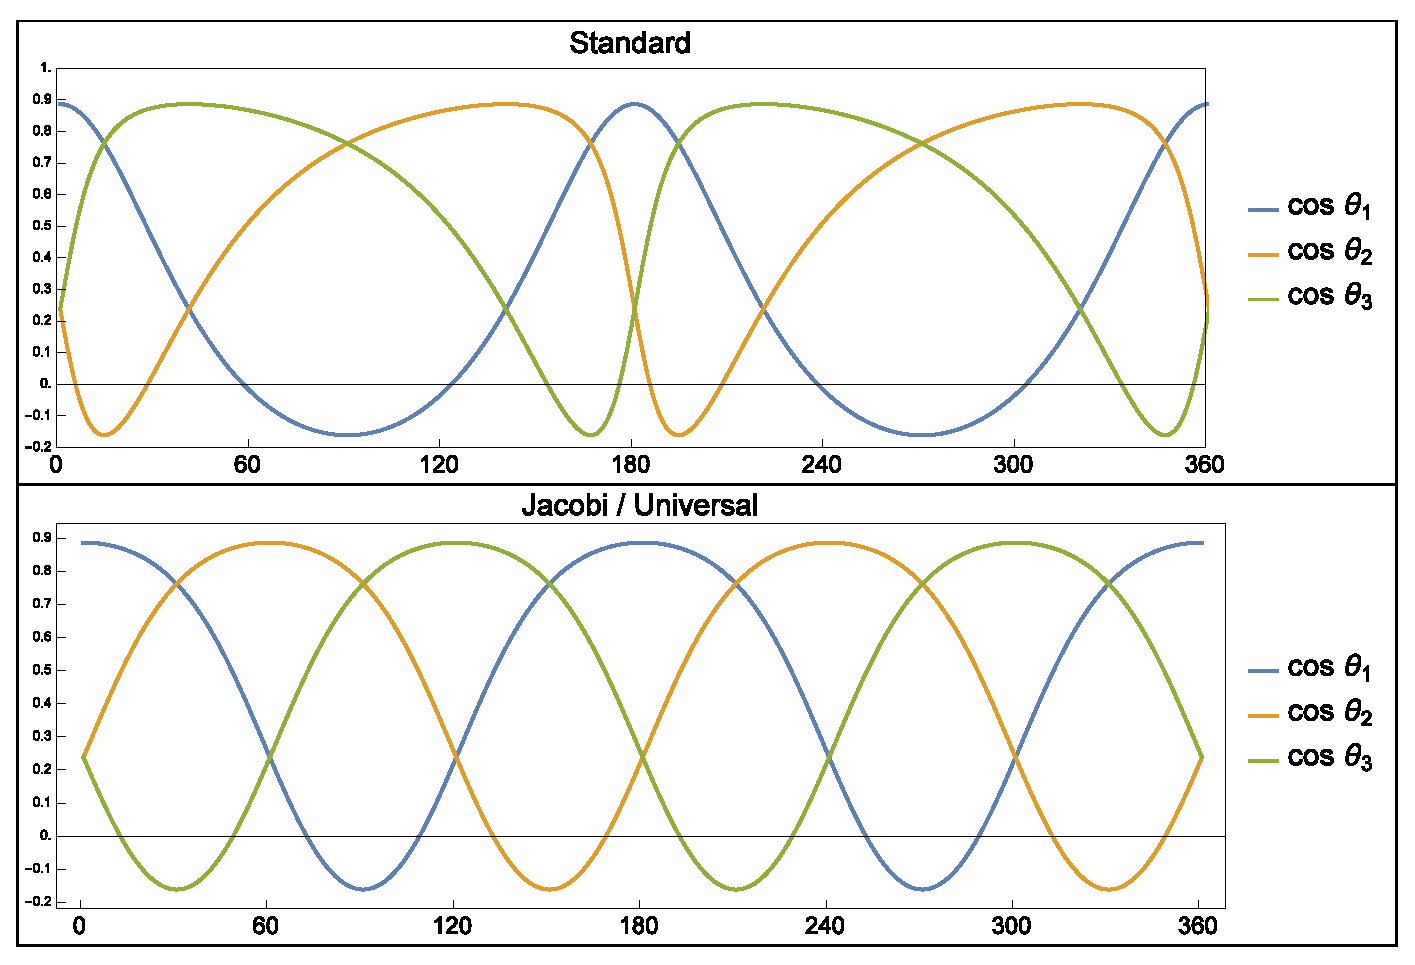
\includegraphics[width=\textwidth]{pics_02_060_cos_parametrizations}
    \caption{The cosines $\cos(theta_i)$ of billiard 3-periodic internal angles for the standard (top) and Jacobi parametrizations (bottom). While in the former case the three curves are distinct, in the latter case all cosines follow the same curve at different phases.}
    \label{fig:02-jacobi-cos-param}
\end{figure}

\section{Exercises}

\begin{exercise}
\label{ex:02-circumbilliard} 
Referring to \cref{fig:02-circumbilliard}, show that every triangle has a circumbilliard, i.e., an ellipse to which it is inscribed and to which it is a billiard 3-periodic. Compute the axes of said circumbilliard with respect to triangle vertices. 
\end{exercise}

\begin{figure}
    \centering
    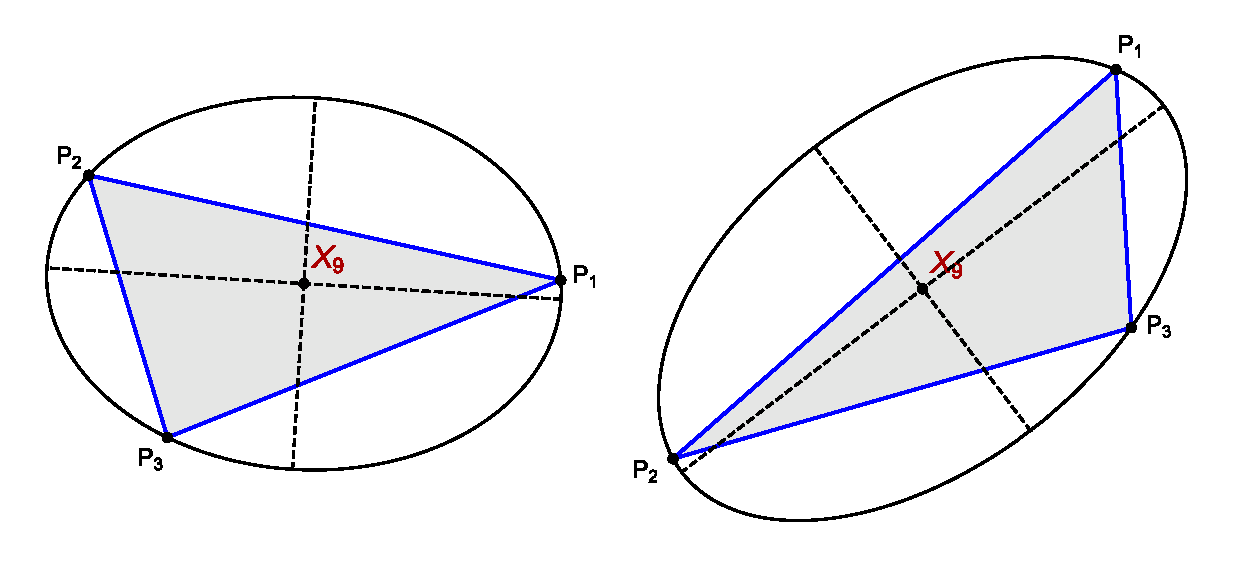
\includegraphics[width=.8\textwidth]{pics_02_910_circumplot.eps}
    \caption{Two random triangles shown with their circumbilliards. \href{https://youtu.be/vSCnorIJ2X8}{Video}}
    \label{fig:02-circumbilliard}
\end{figure}

\begin{exercise}
A pair of circles uniquely defines a {\em pencil} of coaxial circles; see \cite[Limiting Points]{mw}. The pencil contains exactly two circles which degenerate to a point, known as {\em limiting points}. Derive the location of such points for the poristic pair obtained from the image of two confocal ellipses centered at $[0,0]$ and with axes $a,b$ and $a',b'$.
\end{exercise}

\begin{exercise}
Let $\ell_1,\ell_2$ be the limiting points of the two circles which are polar images of a confocal pair $\E,\E'$ with respect to a circle centered on $f_1$. At what aspect ratio $a/b$ of $\E$ will $\ell_2$ coincide with $f_2$?
\end{exercise}

\begin{exercise}
A well-known result is that the inversion of a circle pair $\Cm,\Cm'$ with respect to a circle $\Cm_1$ centered on $\ell_1$ (resp. $\Cm_2$ centered on $\ell_2$) is a pair of concentric circles $\Cm_1'$ and $\Cm_1''$ (resp. $\Cm_1'$ and $\Cm_1''$). Prove the following lesser known result: the ratio of radii between $\Cm_1'$ and $\Cm_1''$ is the same as the ratio between $\Cm_2'$ and $\Cm_2''$. 
\end{exercise}


\begin{figure}
    \centering
    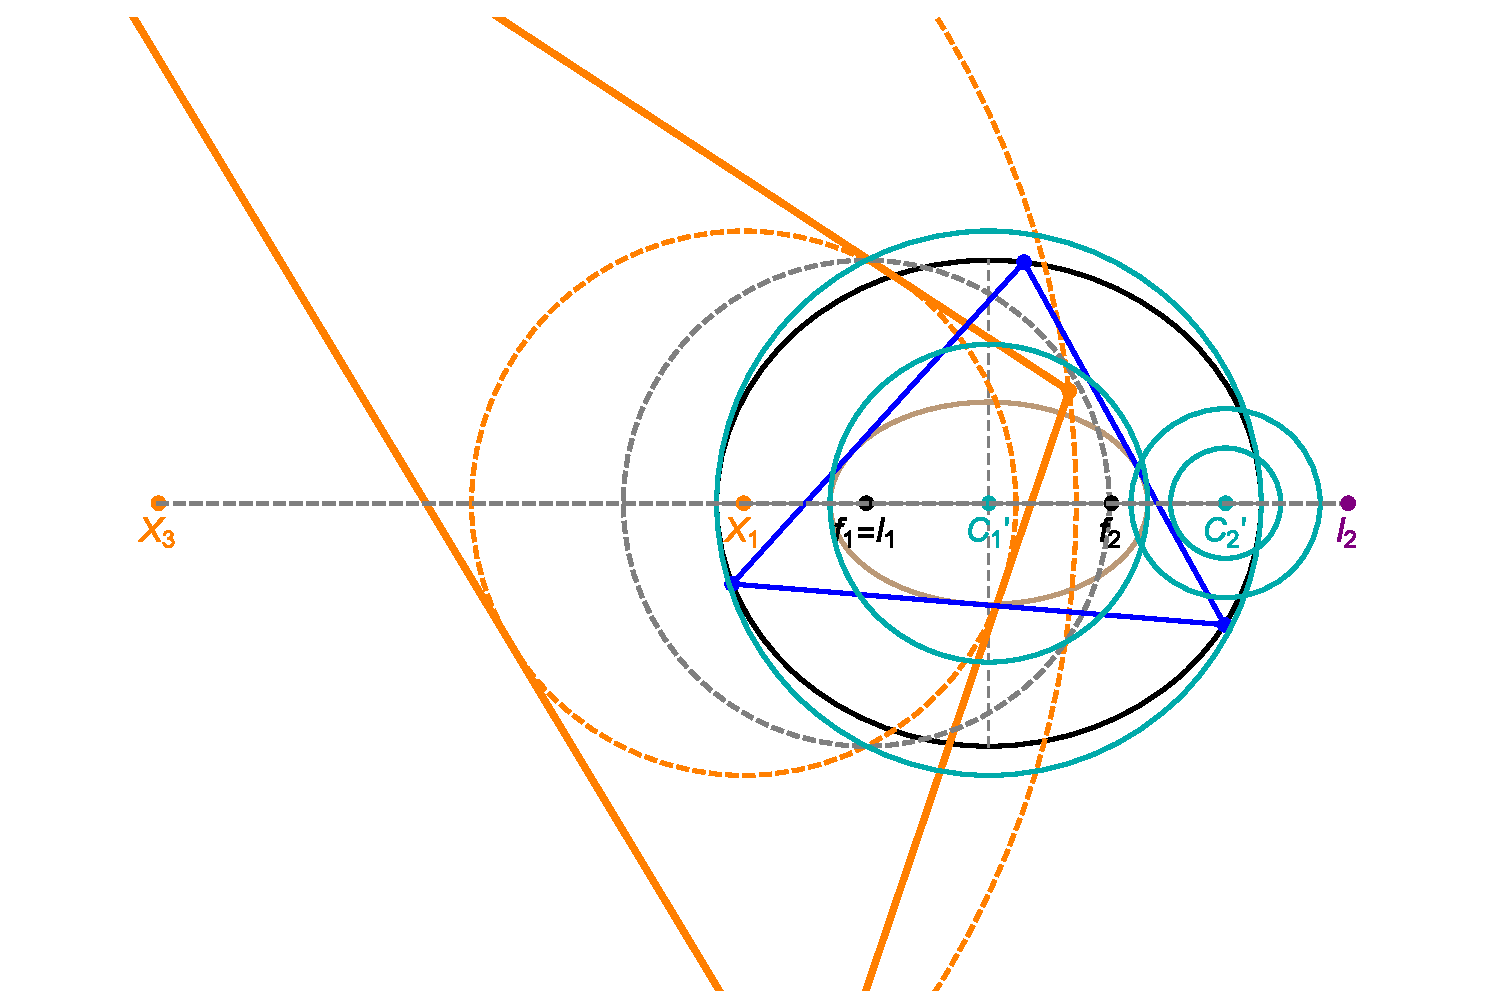
\includegraphics[width=.8\textwidth]{pics_02_920_concentric_inverted_pairs.eps}
    \caption{Concentric circle pairs (light blue) which are the inversions of the circumcircle and incircle (dashed orange) of the bicentric family  (blue) with respect to its two limiting point $\ell_1$ and $\ell_2$. Also shown are Billiard 3-periodics (blue) in the polar pre-image with respect to a circle (dashed gray) -- centered on $f_1=\ell_1$.}
    \label{fig:02-concentric-inverted}
\end{figure}

\begin{exercise}
Referring to \cref{fig:02-concentric-inverted}, let $\Cm,\Cm'$ be the pair of circles which are the polar image of a confocal pair of ellipses $\E,\E'$. Let $\Cm_1', \Cm_1''$ be the inversive images of $\Cm,\Cm'$ wrt to a circle centered on a focus of the ellipse pair. Prove that: (i) $\Cm_1'$ and $\Cm_1''$ are concentric with the ellipse pair and (ii) $\Cm_1'$ (resp. $\Cm_1''$) is externally tangent to $\E$ (resp. $\E'$) at its left and right major vertices.
\end{exercise}


\begin{exercise}
Prove the inversive image of billiard 3-periodics with respect to a focus-centered circle is a non-Ponceletian family inscribed in Pascal's Limaçon whose Gergonne point $X_7$ is stationary; see it \href{https://bit.ly/3edwKD7}{Live}. Indeed, this family has constant perimeter (to be shown later).
\end{exercise}

\begin{exercise}
 Consider the ellipse $x^2/a^2+y^2/b^2=1$. For a  3-periodic  billiard orbit with vertices $P_i=[x_i,y_i]$ (i=1,2,3)  show that:  

\[ 
 \left( x_2\,y_3-x_3\,y_2 \right) x_1\,
y_1+ \left(x_3\,y_1  - x_1\,y_3\right) x_2\, y_2+ \left( x_1\,y_2-x_2\,y_1 \right) x_3
\,y_3=0
\]

\end{exercise}

\begin{exercise} For a  3-periodic  billiard orbit with vertices $P_i=[x_i(t),y_i(t)]$ (i=1,2,3)
Let $C_i(t)=[1/x_i(t),1/y_i(t)]$. 
%Here $P_i(t)=[x_i(t),y_i(t)]$.

Show that the polygon $\{C_1(t),C_2(t),C_3(t)\}$ is a segment that can be bounded or unbounded.
 \label{exe:chap02-inverse-envelope}
\end{exercise}

\begin{exercise} Which simple or self-intersected $N$- gon (closed polygon with $N$ vertices and $N$ sides) can be an orbit on an elliptic billiard? 

 For $N=4$ only the parallelogram can be a non self-intersected orbit on an elliptic billiard, see \cite{connes07}. For the analysis of self-intersected $4-gons$ see \cite{garcia2020-self-intersected}.
\end{exercise}

\begin{exercise}
 Consider a 3-periodic billiard orbit and its antipodal orbit. Show that the six points of intersections of the two triangles are contained in a stationary confocal ellipse $\mathcal{E}_h$: $x^2/a_h^2+y^2/b_h^2=1$ where:


\begin{align*}
	a_h=& {\frac { \left(  \delta -b^2\right) \left( {a}^{2}+{b}^{2}+2\,\delta \right)\sqrt {2\delta-{a}^{2}-{b}^{2} 
			 }  }{3 \left( {a}^{2}-{
				b}^{2} \right) ^{2}}}\\
	%
b_h=&  \,{\frac {\left( {a}^{2}-\delta \right)  \left( {a}^{2}+{b}^{2}+2\,\delta \right) \sqrt {2\delta -{a}^{2
			}-{b}^{2} } }{3 \left( {a}^{2}-
		{b}^{2} \right) ^{2}}}
%
\end{align*}
Conclude that the pair of ellipses $\{\mathcal{E}_h, \mathcal{E}_1\}$ is a billiard pair having all orbits of period 6.
Also show that the pair $\{\mathcal{E} , \mathcal{E}_h \}$ defines a zig-zag billiard and that the orbits have period 12 and  that the perimeter is  constant. %See Fig. \ref{fig:6zigzag}.
\end{exercise}

\section{Research Questions}

\begin{question}
Recall the extouch triangle has vertices at the points of contact of the excircles with a triangle's sidelines \cite[Extouch triangle]{mw}. 
In \cref{chap:05-confocal-loci} we show that the vertices of the extouch triangles of billiard 3-periodics coincide with the caustic touchpoints, see it 
\href{https://bit.ly/33PufRv}{Live}. Show that said extouch family is also Ponceletian and concentric with the elliptic billiard; derive expressions for the semi-axes of its elliptic caustic. Is its center a triangle center? 
\label{que:02-extouch}
\end{question}

\section{Research Questions}

\begin{question}
Recall the extouch triangle has vertices at the points of contact of the excircles with a triangle's sidelines \cite[Extouch triangle]{mw}. 
In \cref{chap:05-confocal-loci} we show that the vertices of the extouch triangles of billiard 3-periodics coincide with the caustic touchpoints, see it 
\href{https://bit.ly/33PufRv}{Live}. Show that said extouch family is also Ponceletian and concentric with the elliptic billiard; derive expressions for the semi-axes of its elliptic caustic. Is its center a triangle center? 
\label{que:02-extouch}
\end{question}


\chapter{Concentric, Axis-Parallel (CAP)}
\label{chap:03-n3-cap}
\section{Introduction}
\label{sec:03-intro}

Reader used to projective geometry may find it redundant to list so many Poncelet family cases. However, locus phenomena are euclidean.

\subsection*{History of the Results}

Early videos 2011 com Jair Koiller \cite{dsr_vid11incenter,dsr_vid11e}, proof by complexification \cite{olga14}, proof by Affine Curvature \cite{garcia2019-incenter}, circumcenter \cite{corentin2021-circum}. Centers of Mass of Poncelet Polygon \cite{schwartz2016-com}, Circumcenter of Mass \cite{sergei2014-circumcenter-of-mass}.

\section{The Confocal Family (Elliptic Billiard)}
\label{sec:03-billiard}
\begin{figure}
    \centering
    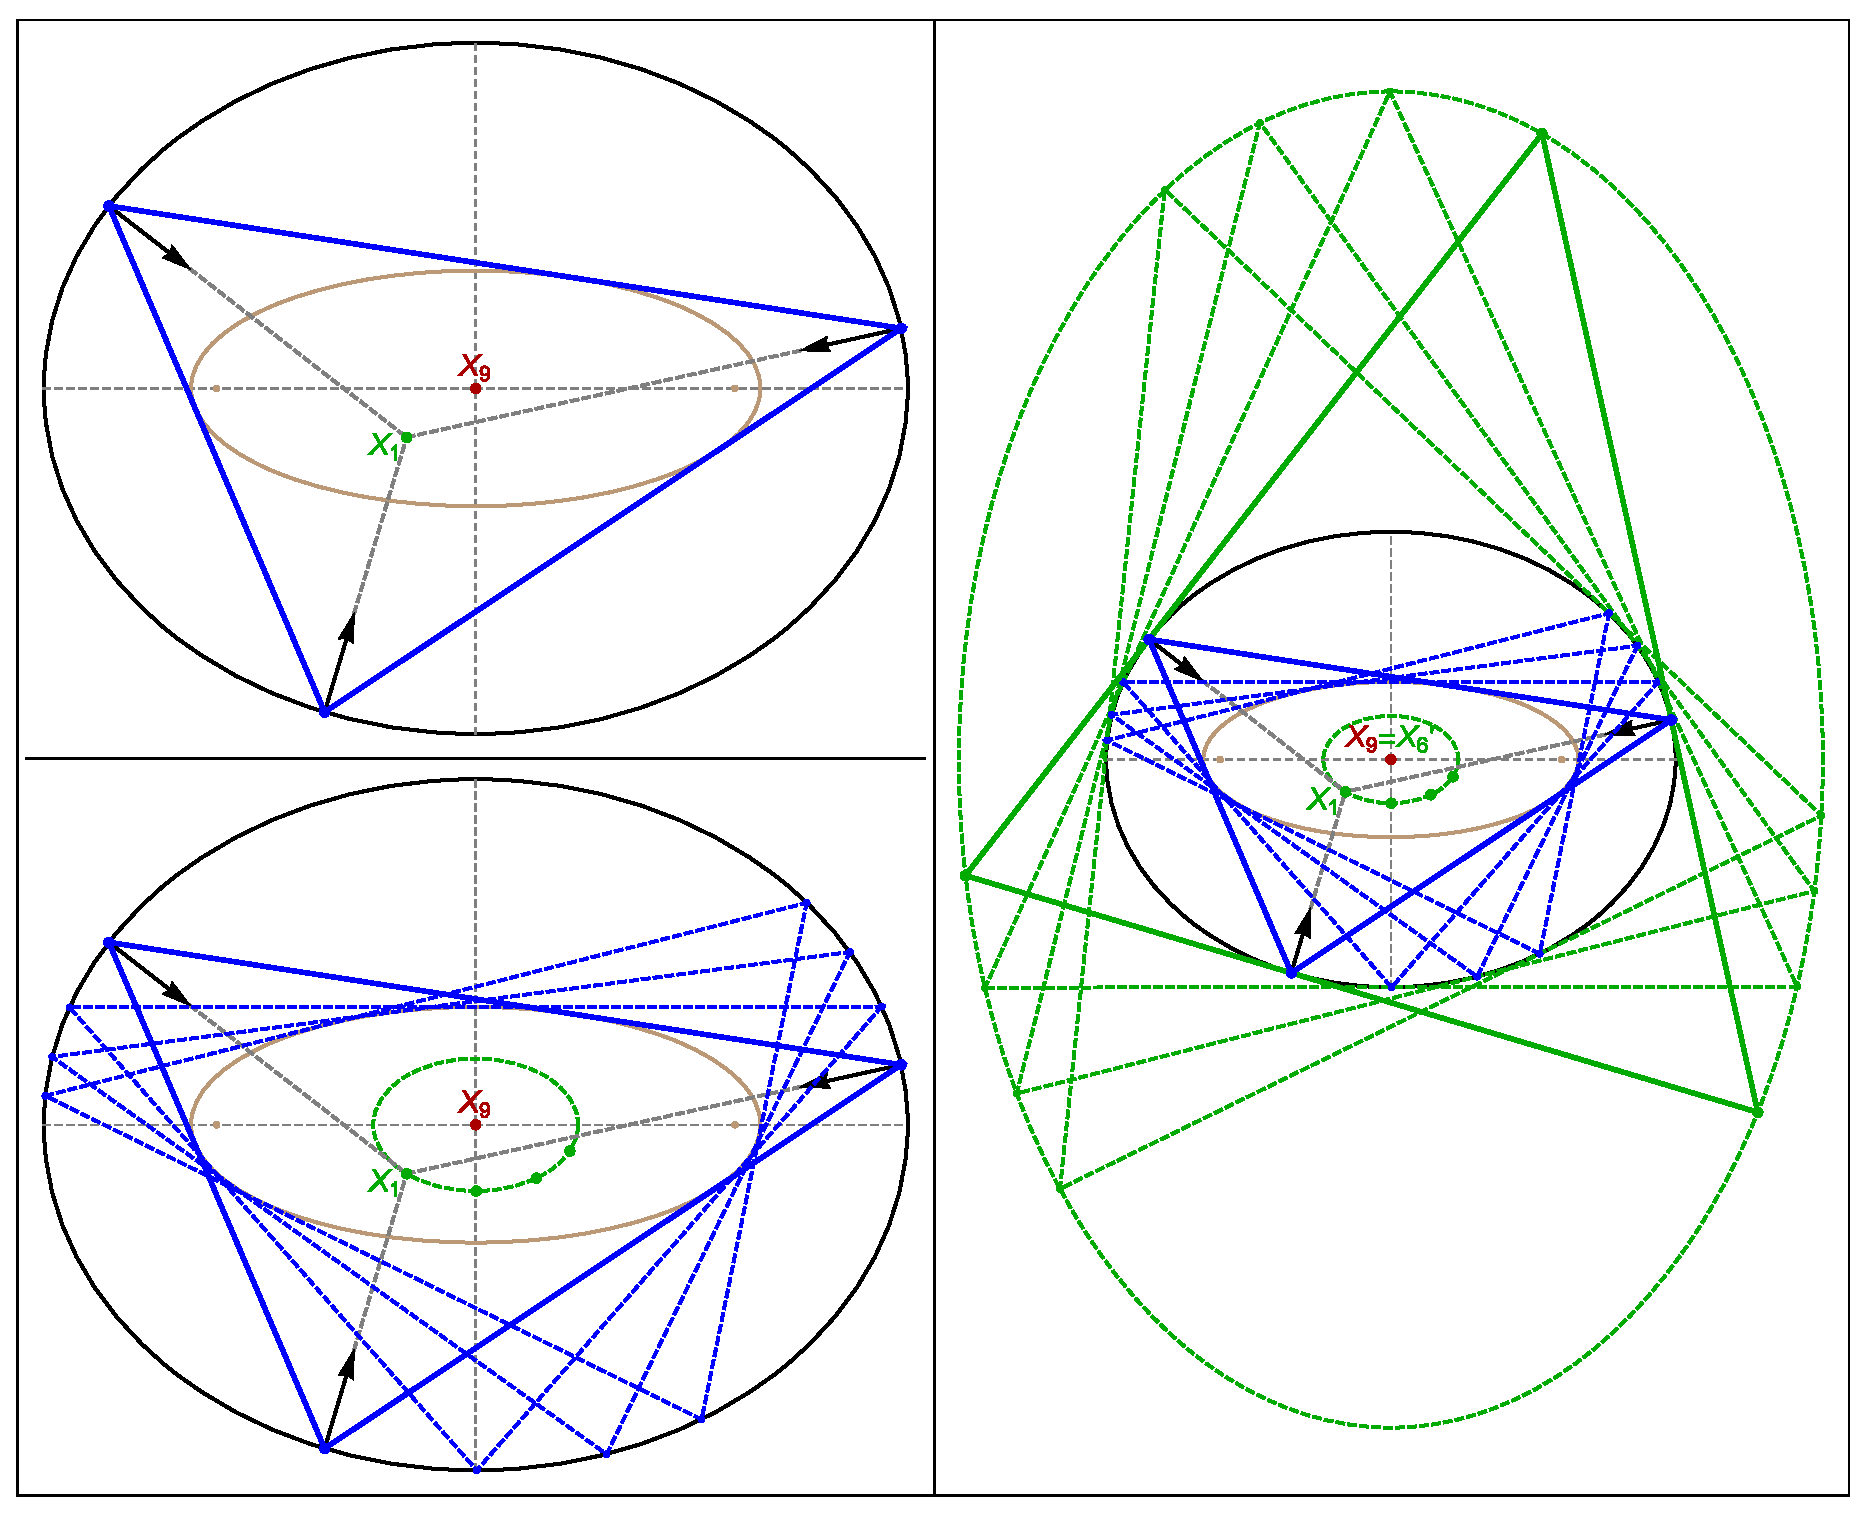
\includegraphics[width=\textwidth]{pics_03_080_billiard_grid.eps}
    \caption{\textbf{Top Left:} An elliptic billiard 3-periodic (solid blue) is shown inscribed in an outer ellipse (black) and a confocal caustic (brown). Graves' theorem implies its internal angles will be bisected by ellipse normals (black arrows). Also shown is the incenter $X_1$ defined as the intersection of said bisectors. \textbf{Bottom Left:} Poncelet's porism implies a 1d family of such triangles exists. Some samples are shown (dashed blue). A classic invariant is  perimeter. The Mittenpunkt $X_9$ remains stationary at the center. The incenter $X_1$ sweeps an ellipse (dashed green). \textbf{Right:} The excentral triangle (solid green) has sides perpendicular to the bisectors. Over billiard 3-periodics, the excentral is of variable perimeter. Its vertices (known as the ``excenters'') also sweep an ellipse (dashed green) whose aspect ratio is the reciprocal of that of the incenter locus. The Symmedian point $X_6'$ of the excentral triangle coincides with $X_9$ of the reference and is therefore stationary. \href{https://bit.ly/3gWl3CI}{Live}}
    \label{fig:billiard-grid}
\end{figure}

Henceforth let {\em billiard 3-periodics} refer to the 1d family of Poncelet triangles interscribed between pair of confocal ellipses $\E$ and $\E_c$ given by:
\[ \E:\frac{x^2}{a^2}+\frac{y^2}{b^2}-1=0,\;\;\;\E_c:\frac{x^2}{a_c^2}+\frac{y^2}{b_c^2}-1=0\]
where $c^2=a^2-b^2=a_c^2-b_c^2$.

The Cayley condition for a concentric, axis parallel (CAP) pair of ellipses to admit a 3-periodic family is given by:

\begin{equation} \frac{a_c}{a}+\frac{b_c}{b}=1
\label{eqn:n3-cayley}
\end{equation}

In turn, this constrains the semi-axes of the confocal caustic.

\begin{proposition}
The semi-axes $a_c,b_c$ of the confocal caustic are given by:
\begin{align*}
a_c=&\frac{a\left(\delta-{b}^{2}\right)}{c^2},\;\;\;\;
b_c=\frac{b\left({a}^{2}-\delta\right)}{c^2}\cdot
\end{align*}
where $\delta=\sqrt{a^4-a^2b^2+b^4}$, an oft-occurring quantity, will be henceforth called the Darboux constant.
\label{prop:03-n3-caustic}
\end{proposition}

When $a=b$, we have that $a_c=b_c=a/2$.

\begin{remark}
The semi-axes $a$ and $b$ of the ellipse in terms of the semi-axes $a_c$ and $b_c$ of the confocal ellipse are given by:
\begin{align*}
a&= -\frac{1}{2} \sqrt{w_1} + \frac{1}{2} \sqrt{ w_2 -\frac{ 2 a_c^3 - 4 c^2a_c}{\sqrt{w_1}} } +\frac{a_c}{2},\;\; b=\sqrt{a^2-c^2}\\
w_1&=a_c^2-(4 c a_c b_c)^{\frac{2}{3}},\;\; w_2=2 a_c^2+ (4 c a_c b_c)^{\frac{2}{3}}
\end{align*}
The implicit equation that defines $a$ above is the quartic  given by
\[c^2( a_c^2   - 2   a_c   a )+ a^2(2a_c a  - a^2)=0\]
\end{remark}

Billiard N-periodics classically conserve  perimeter $L$ and Joachimsthal's constant $J$ (see \cref{app:appC-convex-billiard}).
\textcolor{red}{checar ref. de cruzamento acima}
When $N=3$, we can derive these explicitly using the vertex parametrization given in \cref{prop:03-vtx-param}.
 

\begin{proposition}
For billiard 3-periodics, the perimeter and Joachimsthal's constant are given by:

\begin{equation*}
J=\frac{\sqrt{2\delta-a^2-b^2}}{c^2},\;\;\;L=2(\delta+a^2+b^2)J
\label{eqn:n3-L-J}
\end{equation*}
\end{proposition}

\begin{proof} We compute the values considering  an isosceles 3-periodic orbit with $P_1=[a,0]$, and

% {\small  
% \begin{equation}\label{eq:isosceles_3orbit}
%  \;  P_2   =\left[-\frac {{a}^{2}\sqrt {2\,\delta-{a}^{2}-{b}^{2}}}{c^2},   
%	\frac { \left(\delta  -{a}^{2}\right) b}{c^2}\right],\;\;
%	    P_3= \left[{-\frac {{a}^{2}\sqrt {2\,\delta-{a}^{2}-{b}^{2} }}{c^2}},
%	{\frac { \left(  {a}^{2}-\delta \right) %b}{c^2}}\right]
%\end{equation}
 %}%
 {\small 
 \begin{equation} \label{eq:orbita3-isosceles}
 P_2=\left[   {\frac {a \left(  {b}^{2}-\delta \right) }{   a^2-b^2 
 			  }},{\frac {{b}^{2}\sqrt {2 \delta -{a}^{2}-{b}^{2}\,
 				}}{{a}^{2}-{b}^{2}}} 
 	\right], \;\; P_3=\left[  {\frac {a \left(  {b}^{2}-\delta \right) }{   a^2-b^2   
 	}},-{\frac {{b}^{2}\sqrt {2\delta-{a}^{2}-{b}^{2} 
 				}}{{a}^{2}-{b}^{2}}} 
 	\right]
 	\end{equation}
 	}
 	We have that
 	\[L=|P_2-P_3|+2|P_1-P_2|,\;\;
 	 J=\langle \frac{P_1-P_3}{|P_1-P_3|},[\frac{1}{a},0]\rangle\]
 	 Straightforward calculations using the vertex parametrization given in \cref{prop:03-vtx-param}, lead to the stated result.
%\textcolor{red}{ronaldo: CAS+parametrization}
\end{proof}

\noindent Note: the use of $J$ in this chapter refers to its value for the $N=3$ case. Referring to \cref{fig:billiard-grid}:

\begin{theorem}
Over billiard 3-periodics, the locus of the incenter $X_1$ and excenter are ellipses $\E_1$ and $\E_e$ concentric and axis-parallel with the confocal pair whose axes $(a_1,b_1)$ and $(a_e,b_e)$ are given by:
\begin{align*}
a_1 =& \frac{\delta-b^2 }{a},\;\;\;b_1=\frac{a^2-\delta}{b}\\ 
a_e= &\frac{{b}^{2}+\delta}{a},\;\;\;b_e=\frac{{a}^{2}+\delta}{b}
\end{align*}
Furthermore, $\E_1$ and $\E_e$ have reciprocal aspect ratios, i.e., $a_1/b_1=b_e/a_e$.
\label{thm:03-incenter-excenter}
\end{theorem}

\begin{proof}
It follows from the vertex parametrization in \cref{prop:03-vtx-param} and the definition of incenter and excenters.  
We have that
\[X_1=\frac{s_1 P_1+s_2P_2+s_3P_3}{s_1+s_2+s_3}=
\frac{1}{L}(s_1P_1+s_2P_2+s_3P_3)\]
where $s_1=|P_2-P_3|$, $s_2=|P_1-P_3|$ and $s_3=|P_1-P_2|$.
A careful symbolic analysis shows that $\mathcal{E}_1(X_1)=0$. A similar analysis considering the excenters shows that the locus of the three points is the ellipse $\mathcal{E}_e$ stated.
\end{proof}

\begin{remark} Given the semi-axes $a_e$, $b_e$ of $\mathcal{E}_e$ it follows that semi-axes $a$, $b$ of the caustic $\mathcal{E}$ are given by
\[a=\frac{(\delta_1- a_e^2 - 3b_e^2) a_e}{2(a_e^2 -  b_e^2)},\;\; b=\frac{(3a_e^2 + b_e^2 - \delta_1)b_e}{2(a_e^2 - b_e^2)},\;
  \delta_1=\sqrt{a_e^4 + 14a_e^2b_e^2 + b_e^4}\]

\end{remark}
\textcolor{red}{Feito:  acima. ronaldo consegue inverter, ou seja dados os semi-eixos externos $a_e$, $b_e$, quais são $a_c,b_c$ (bilhar)}

\begin{corollary}
The pair $\{\mathcal{E},\mathcal{E}_e\}$ is Ponceletian.
\label{cor:03-excentral-billiard-poncelet}
\end{corollary}

\begin{proof}
Direct from Cayley condition
\[\frac{a}{a_e}+\frac{b}{b_e}=\frac{a^2}{b^2+\delta}+\frac{b^2}{a^2+\delta}= 1\]

\end{proof}

It turns out $\delta$ has a curious geometric interpretation. Recall the power of a point $Q$ with respect to a circle $\Cm=(C_0,R_0)$ is given by $|Q-C_0|^2-R_0^2$, see \cite[Circle Power]{mw}. Let $\Cm$ denote the (moving) circumcircle of billiard 3-periodic, and $O=X_9$ the billiard center.

\begin{proposition}
The power of $O$ with respect to $\Cm$ is constant and equal to $-\delta$.
\end{proposition}

\begin{proof}
Consider an isosceles 3-periodic orbit given by \cref{eq:orbita3-isosceles}.  
  
	Its circumcircle will be centered at $C_0=[ {\frac { {b}^{2}-\delta}{2b}},0]$ with circumradius $R_0=\frac {{b}^{2}+\delta}{2b}.$
	Therefore, the power of the center of the ellipse with respect to the circumcircle is given by  
	$$|OC_0|^2-R_0^2=\left(\frac { {b}^{2}-\delta}{2b}\right)^2 - \left(\frac {{b}^{2}+\delta}{2b}\right)^2=-\delta.$$
	
	For a generic 3-periodic orbit, the stated invariance is confirmed with a CAS using the vertex parametrization in \cref{prop:03-vtx-param}.  
%	\textcolor{red}{localizar depois}
\end{proof}

The Mittenpunkt $X_9$ is a triangle center where lines from each excenter thru the side midpoint meet. Referring to \cref{fig:03-x9}:
\begin{theorem}
Over the family of 3-periodics in the elliptic billiard, $X_9$ is stationary at the common center.
\end{theorem}

An elegant syntethic proof was kindly contributed by \cite{olga19_mitten}:

\begin{proof}
Let $\E$ be the outer ellipse in the confocal pair, $O$. By definition, the Mittenpunkt $X_9$ is where lines from the excenters $E_i$ through the side midpoints $M_i$ concur. Notice each side is an ellipse chord between tangents to $\E$ seen from the $E_i$ (this is because in the confocal pair the excentral triangle is tangent to $\E$). Consider the image of lines $E_i M_i$ under an affine transform which sends $\E$ to a circle $\Cm'$, let $O'$ be its center. The transformed lines will pass through the midpoints of chords of $\Cm'$ between tangents seen from $E_i'$ (the affine image of $E_i$). By circular symmetry, such lines must also pass through $O'$, and therefore remain stationary. But $O'$ is the affine image of $O$, so the result follows.
\end{proof}

\begin{figure}
     \centering
    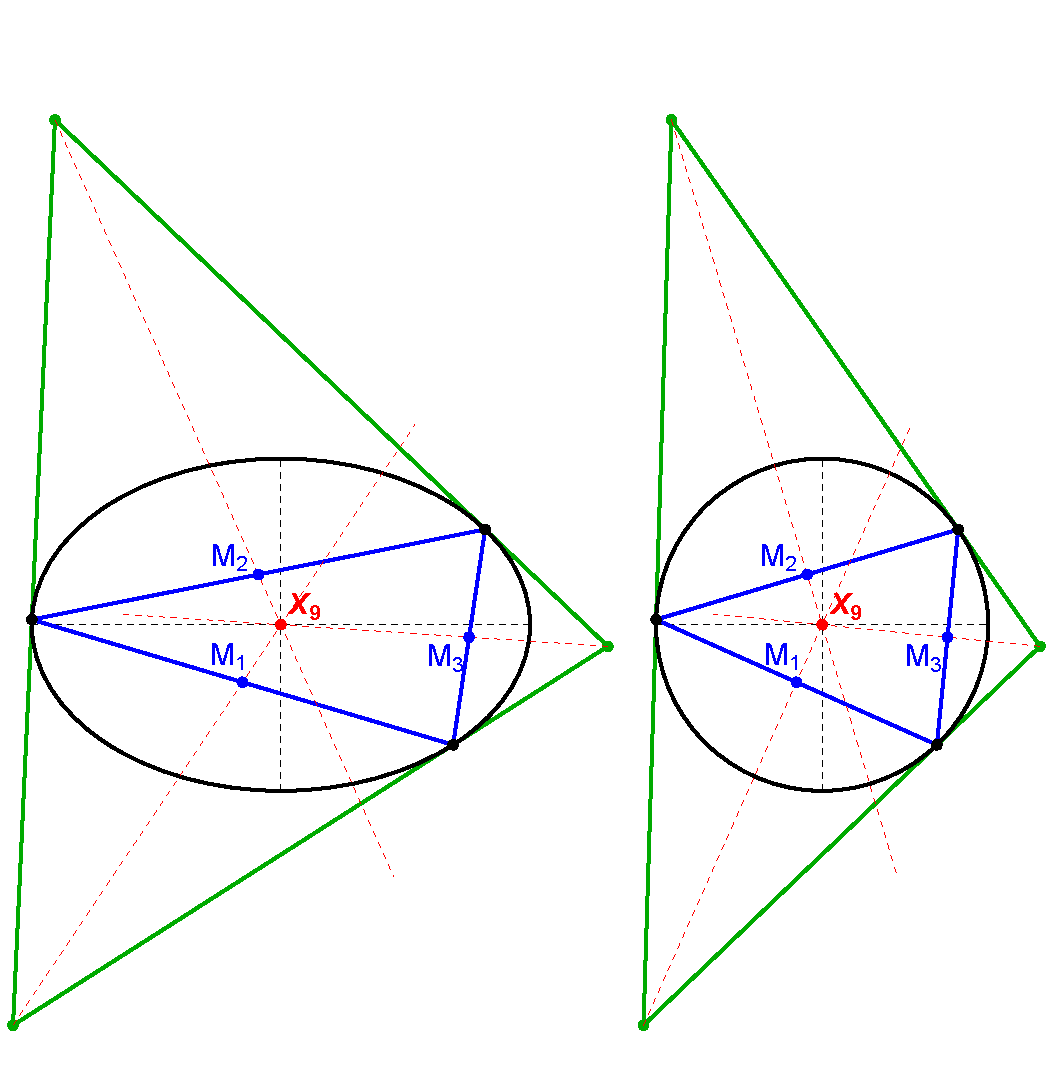
\includegraphics[width=\linewidth]{pics_03_090_mitten_proof.pdf}
     \caption{\textbf{Left}: 3-periodic billiard triangle (blue), its excentral triangle (green). The Mittenpunkt $X_9$ is the point of concurrence of lines drawn from the excenters through sides' midpoints $M_i$. \textbf{Right}: the affine image which sends the billiard to a circle. Lines from imaged excenters through sides' midpoints must pass through the origin. Since the latter is stationary, so must be its pre-image $X_9$, which is stationary at the billiard center.  % done
     \href{https://youtu.be/tMrBqfRBYik}{Video}}
     \label{fig:03-x9} 
\end{figure}

Given a triangle, let $r$ and $R$ denote the radius of its incircle and circumcircle, known as the {\em inradius} and {\em circumradius}, respectively. Over billiard 3-periodics, note these two radii are variable. Referring to \cref{fig:radii}:

\begin{theorem}
$r/R$ is invariant over the 3-periodic orbit family and given by:
\begin{equation*}
\label{eqn:rovR}
\frac{r}{R}=\frac{2 (\delta-b^2)(a^2-\delta)}{c^4}.
\end{equation*}
\label{thm:03-confocal-rovR}
\end{theorem}

\begin{proof}
The following relation, found in \cite{johnson1960}, holds for any triangle:

\begin{equation*}
 r R=\frac{s_1s_2s_3}{2 L}, 
\end{equation*}

\noindent where $L=s_1+s_2+s_3$ is the perimeter, constant for 3-periodic orbits. Therefore:

\begin{equation}
\frac{r}{R}=\frac{1}{2L} \frac{s_1s_2s_3}{R^2}\cdot
\label{eqn:rovR-cas}
\end{equation}

Next, let $P_1=(a,0)$ be a vertex of an isosceles 3-periodic. Obtain a candidate expression for $r/R$. This yields \eqref{eqn:rovR} exactly. Using the vertex parametrization in \cref{prop:03-vtx-param}, derive an expression for the square of the right-hand side of \eqref{eqn:rovR-cas} as a function of $x_1$ and subtract from it the square of \eqref{eqn:rovR}. In  \cite{garcia2020-new-properties}
it is shown $\left(s_1s_2s_3/R^2\right)^2$ is rational on $x_1$. For simplification, use $R=s_1 s_2 s_3/(4A)$, where $A$ is the triangle area. With a CAS, show said difference is identically zero for all $x_1\in(-a,a)$.
\end{proof}


\begin{figure}
    \centering
    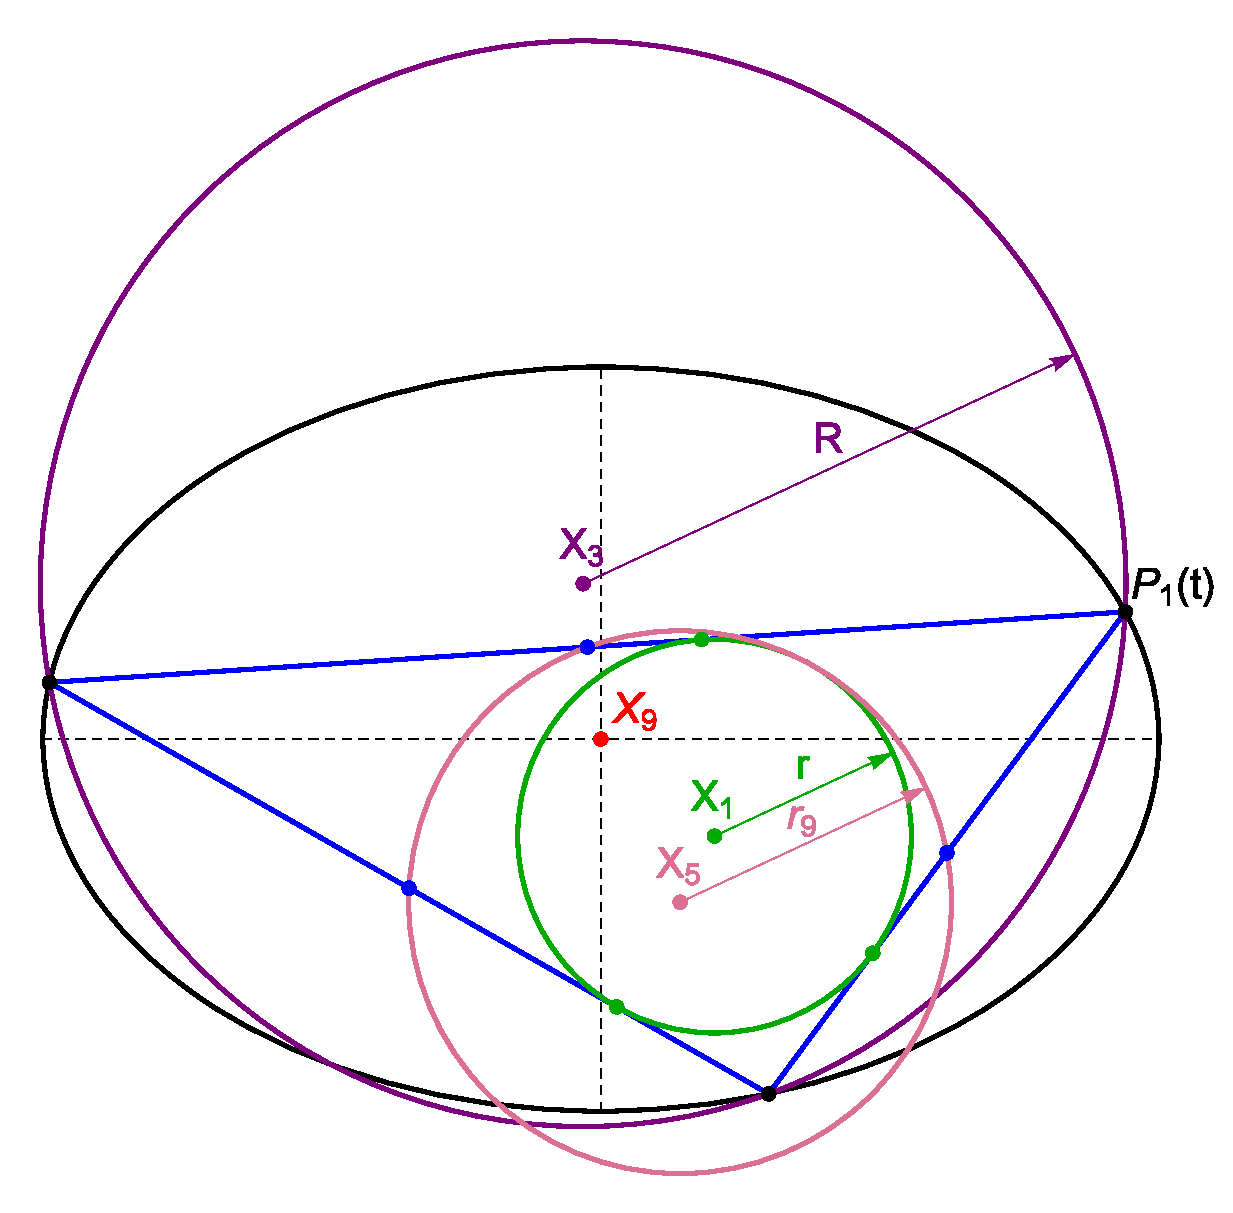
\includegraphics[width=\textwidth]{pics_03_100_radii}
    \caption{The incircle (green), circumcircle (purple), and 9-point (Euler's) circle (pink) of a billiard triangle (blue). These are centered on $X_1$, $X_3$, and $X_5$, respectively. Their radii are the inradius $r$, circumradius $R$, and 9-point circle radius $r_9=2R$. Over the family, the ratio $r/R$ is invariant. In turn this implies an invariant sum of cosines. \href{https://bit.ly/337hvpf}{Live}}
    \label{fig:radii}
\end{figure}

Let $\theta_i$, $r$, $R$, and $A$ denote the ith internal angle, inradius, circumradius, and area of a reference triangle. Primed quantities refer to the excentral triangle. The relations below, appearing in  \cite{johnson1960},  hold for any triangle:

\begin{align}
\sum_{i=1}^{3}{\cos\theta_i}&=1+\frac{r}{R} \label{eqn:03-sum-cos} \\
\prod_{i=1}^{3}{\cos\theta_i'}&=\frac{r}{4R} \label{eqn:03-exc-prod-cos} \\
\frac{A}{A'}&=\frac{r}{2R} \label{eqn:03-area-ratio}
\end{align}

\begin{corollary}
Over billiard 3-periodics, also invariant are the sum of the orbit cosines, the product of excentral cosines, and the ratio of excentral-to-orbit areas.
\label{cor:03-rOvR}
\end{corollary}

Direct calculations yields an expression for the invariant sum of cosines in terms of elliptic billiard constants $J$ and $L$.

\begin{corollary}
$\sum_{i=1}^{3}{\cos\theta_i}=J L - 3$
\end{corollary}

At it will be seen later in \cref{chap:05-billiard}, the above generalizes to $J L -N$ for all $N$.

\section{Vertex Parametrization with Jacobi's Elliptic Functions}
 
 
\subsection{A generic CAP pair}

Consider a general pair of CAP ellipses denoted $\E$ and $\E_c$. We will derive a generic parametrization for the vertices of 3-periodics in such a pair. A first calculation will be helpful. Referring to \cref{fig:ell-ints}(left), the following are coordinates for the intersections $P_2$ and $P_3$ on $\E$ of the two tangents to $\E_c$ seen from a point $P_1=[x_1,y_1]$ also on $\E$:

\begin{figure}
    \centering
    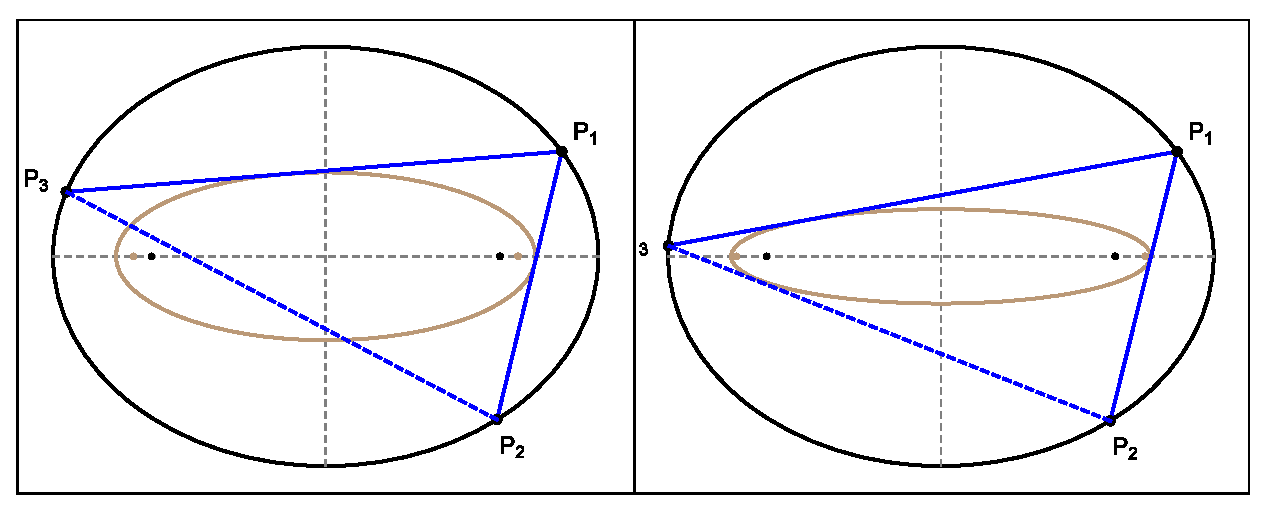
\includegraphics[width=\textwidth]{pics_03_070_ell_ints.eps}
    \caption{\textbf{Left:} Two CAP ellipses (black and brown), and a point $P_1$ on the outer one. The lines thru $P_1$ tangent to the inner ellipse intersect the outer one at $P_2$ and $P_3$. Notice that $P_2 P_3$ cut thru the inner ellipse, i.e., the pair of ellipses does not satisfy Cayley's conditions. \textbf{Right:} the minor axis of the inner ellipse has been scaled such that $P_1 P_2 P_3$ is now a Poncelet triangle.}
    \label{fig:ell-ints}
\end{figure}

\begin{align}
    P_2& =[x_2,y_2]=\frac{1}{k_2}\left[\frac{u_1 x_1 + u_2 y_1}{b} ,  \frac{w_1 x_1 + w_2 y_1}{a} \right] \label{eq:03-n3-conc-general} \\
    P_3&=[x_3,y_3]=\frac{1}{k_2}\left[\frac{w_1 x_1 - w_2 y_1}{b},\frac{w_1 x_1 - w_2 y_1}{a}\right] \nonumber
\end{align}
where:
\begin{align*}
    u_1 &=b\left(a^4  b_c^4 -(a^2 -  a_c^2)^2 b^4 \right) \\
    u_2 &= 2 a k_1 \left( (a^2 + a_c^2)b^2 - b_c^2 a^2\right) \\
    k_1&=\sqrt{ b^2  b_c^2 (a^2 -  a_c^2)  x_1^2 +  a_c^2 a^2(b^2 -  b_c^2)  y_1^2}\\
    k_2 &=\left(\frac{a^2 (b^2 +  b_c^2) - a_c^2 b^2 }{a}x_1\right)^2+ \left(\frac{a^2 (b^2 -  b_c^2) + a_c^2b^2 }{b} y_1\right)^2\\
    w_1&=2 b k_1\left( (b^2 +  b_c^2) a^2 - a_c^2 b^2\right) \\
    w_2&= a\left(a_c^4b^4-a^4(b^2-b_c^2)^2\right)
     %=-a (a^2( b^2 -    b_c^2) -  a_c^2 %b^2) (a^2 (b^2 -   b_c^2) +  a_c^2 b^2)
\end{align*}
 
\subsection{Brocard Porism}

Consider an isosceles Poncelet triangle $\Tm=ABC$ in the Brocard porism, where $AB$ is tangent to $\E$ at one of its minor vertices. Let $|AB|=2d$ and the height be $h$. Let $\zeta=d^2+h^2$. Let the origin $(0,0)$ be at its circumcenter $X_3$. Its vertices will be given by:

\[A=\left[-d ,\frac{d^2-h^2}{2h}\right], \;\;\; B= \left[d,\frac{d^2-h^2}{2h}\right], \;\;\; \left[0 ,\frac{\zeta}{2h}\right] \]


\begin{proposition}\label{prop:pair_brocard}
The Brocard porism containing $\Tm$ as a Poncelet triangle is defined by the following circumcircle $\K_0$ and Brocard inellipse $\E$:

\begin{align*}
\K_0:& x^2+y^2-R^2=0, \;\;\; R=\frac{\zeta}{2h}\\
\E:& -64d^2  h^4  x^2-4  h^2  (9  d^2+h^2)  \zeta  y^2 +4  h  (3  d^2+h^2)  (3  d^2-h^2)  \zeta  y\\&-(d^2-h^2) (9d^2 -h^2) \zeta^2=0
\end{align*}
\end{proposition}

\begin{proof}
The proof follows from $\Tm$, and isosceles Poncelet triangle. Recall that the Brocard inellipse is centered at $X_{39}$. Its perspector is $X_6$, i.e., it will be tangent to $\Tm$ where cevians through $X_6$ intersect it; see \cite[Brocard inellipse]{mw}.
\end{proof}


Consider the pair: circle $x^2+y^2=R^2=(d^2+h^2)^2/(4h^2)$ and   ellipse
$x^2/a^2+(y-y_0)^2/b^2=1$, with  semi-axes
 \[  (a,b)=\left(\frac{d\sqrt{d^2+h^2}}{9d^2+h^2},\frac{4d^2}{9d^2+h^2}\right)
    \]
and center $(0,y_0)$,  $y_0=(9d^4 - h^4)/(2h(9d^2  +  h^3))$.

Vertices $P_i=[x_i,y_i]$, $i=1,2,3$ of Brocard porism triangles are given by:

{\small  
\begin{equation}
    \aligned
    x_1 &= \cos{t}/q_1\\
    y_1 &= \sin{t}/q_1 \\
    x_2 &= -d (d^2 + h^2) ((3 d^2 + h^2)\sin{t} + 2d h \cos{t}- 3 d^2 + h^2)/q_2 \\
    y_2&=-(d^2 + h^2) ((9 d^4 - 2 d^2 h^2 + h^4)\sin{t} - 2 d h (3 d^2 + h^2)\cos{t} - 9 d^4 + h^4)/(2 b q_2) \\
    x_3 &= d (d^2 + h^2) (2 d h \cos{t} - (3 d^2 + h^2) \sin{t} + 3 d^2 - h^2)/q_3\\
    y_3 &=(d^2 + h^2) (2d h (3 d^2 + h^2) \cos{t}+ (9 d^4 - 2 d^2 h^2 + h^4)\sin{t} - 9 d^4 + h^4)/(2 b q_3) \\
    q_1&=(2h)/(d^2+h^2)\\
    q_2&= 2 d h (3 d^2 - h^2)\cos{t} - (9 d^4 - h^4) \sin{t}  + 9 d^4 + 2 d^2 h^2 + h^4\\
    q_3&= 2 d h (3 d^2 - h^2)\cos{t} + (9 d^4 - h^4)\sin{t} - 9 d^4 - 2 d^2 h^2 - h^4
\endaligned
\label{eqn:03-vertices-brocard}
\end{equation}
}


\textcolor{red}{ronaldo, stachel, pagina observable}

\cite{stachel2021-billiards},\cite{reznik2021-n3-spatiotemporal},\cite{reznik2021-n3-jacobi}

\textcolor{red}{dan: comparar posicao de p1 na parametrizacao natural vs jacobi}

\section{Exercises}

\begin{exercise}
\label{ex:03-circumbilliard} 
Show that every triangle has a circumbilliard, i.e., an ellipse to which it is inscribed and to which it is a billiard 3-periodic. Compute the axes of said circumbilliard with respect to triangle vertices. 
\end{exercise}

\begin{exercise}
A pair of circles uniquely defines a {\em pencil} of coaxial circles; see \cite[Limiting Points]{mw}. The pencil contains exactly two circles which degenerate to a point, known as {\em limiting points}. Derive the location of such points for the poristic pair obtained from the image of two confocal ellipses centered at $[0,0]$ and with axes $a,b$ and $a',b'$.
\end{exercise}

\begin{exercise}
Let $\ell_1,\ell_2$ be the limiting points of the two circles which are polar images of a confocal pair $\E,\E'$ with respect to a circle centered on $f_1$. At what aspect ratio $a/b$ of $\E$ will $\ell_2$ coincide with $f_2$?
\end{exercise}

\begin{exercise}
A well-known result is that the inversion of a circle pair $\Cm,\Cm'$ with respect to a circle $\Cm_1$ centered on $\ell_1$ (resp. $\Cm_2$ centered on $\ell_2$) is a pair of concentric circles $\Cm_1'$ and $\Cm_1''$ (resp. $\Cm_1'$ and $\Cm_1''$). Prove the following lesser known result: the ratio of radii between $\Cm_1'$ and $\Cm_1''$ is the same as the ratio between $\Cm_2'$ and $\Cm_2''$. 
\end{exercise}


\begin{figure}
    \centering
    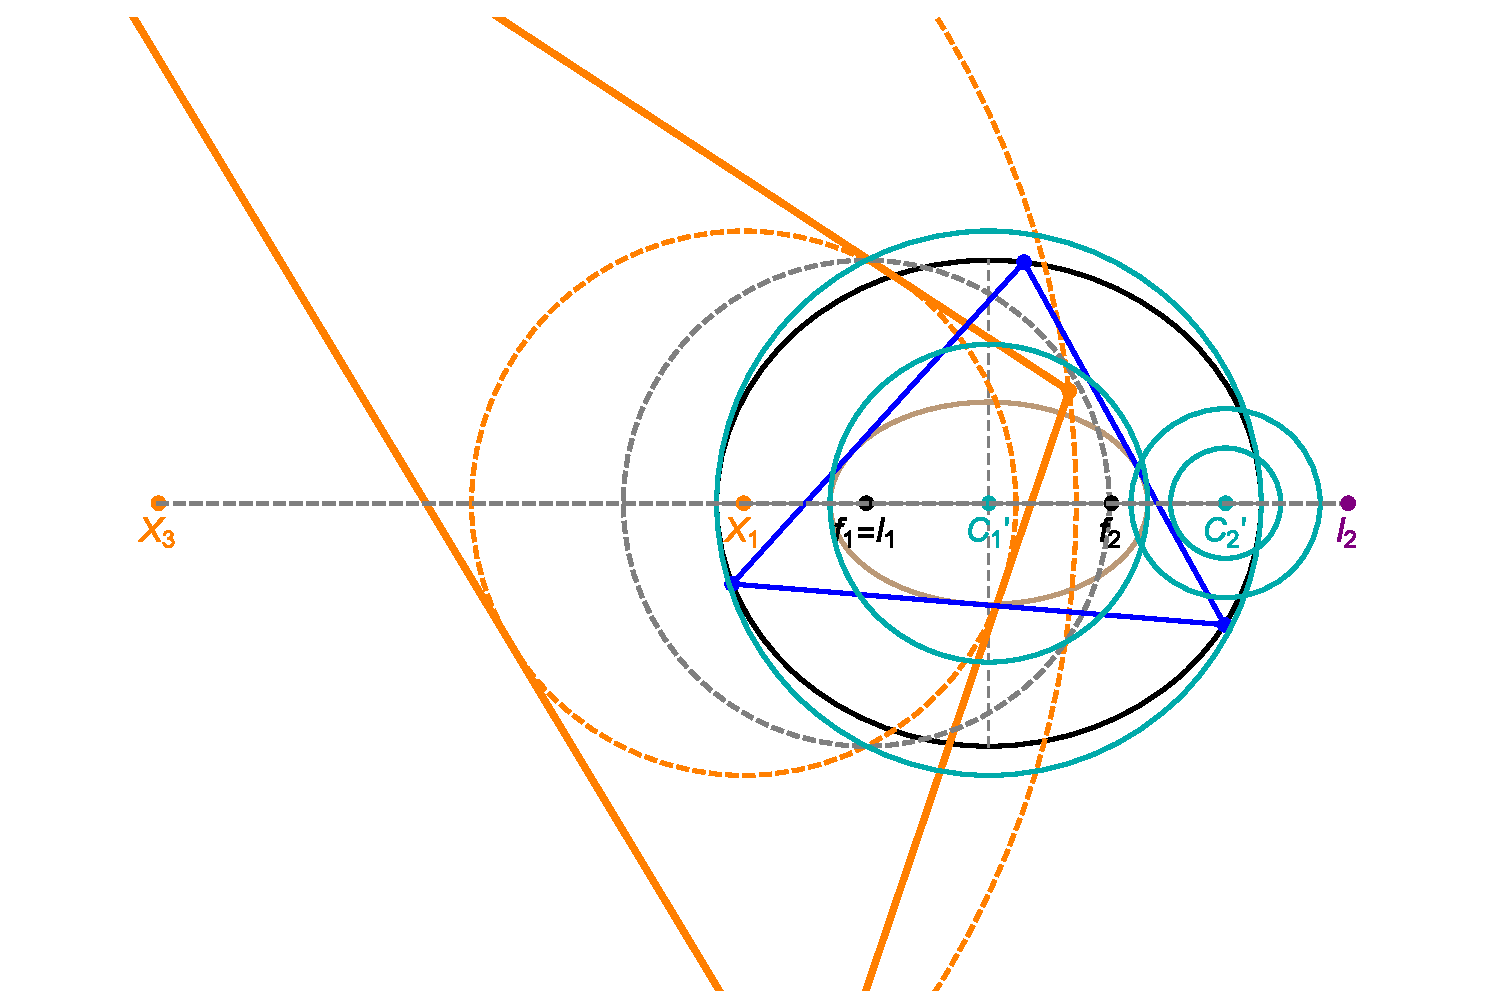
\includegraphics[width=.8\textwidth]{pics_03_210_concentric_inverted_pairs.eps}
    \caption{Concentric circle pairs (light blue) which are the inversions of the circumcircle and incircle (dashed orange) of the bicentric family  (blue) with respect to its two limiting point $\ell_1$ and $\ell_2$. Also shown are Billiard 3-periodics (blue) in the polar pre-image with respect to a circle (dashed gray) -- centered on $f_1=\ell_1$.}
    \label{fig:03-concentric-inverted}
\end{figure}

\begin{exercise}
Referring to \cref{fig:03-concentric-inverted}, let $\Cm,\Cm'$ be the pair of circles which are the polar image of a confocal pair of ellipses $\E,\E'$. Let $\Cm_1', \Cm_1''$ be the inversive images of $\Cm,\Cm'$ wrt to a circle centered on a focus of the ellipse pair. Prove that: (i) $\Cm_1'$ and $\Cm_1''$ are concentric with the ellipse pair and (ii) $\Cm_1'$ (resp. $\Cm_1''$) is externally tangent to $\E$ (resp. $\E'$) at its left and right major vertices.
\end{exercise}


\begin{exercise}
Prove the inversive image of billiard 3-periodics with respect to a focus-centered circle is a non-Ponceletian family inscribed in Pascal's Limaçon whose Gergonne point $X_7$ is stationary; see it \href{https://bit.ly/3edwKD7}{Live}. Indeed, this family has constant perimeter (to be shown later).
\end{exercise}


\section[More concentric Poncelet families]{Other Notable Concentric, Axis-Parallel, Poncelet Families}
\label{sec:03-other-conc}
 Below we introduce five additional notable 3-periodic Poncelet families interscribed between a pair of concentric, axis-parallel (CAP) ellipses. As before, the Cayley condition \cref{eqn:n3-cayley} will be used to constrain the ellipse pair. 

\begin{figure}
    \centering
    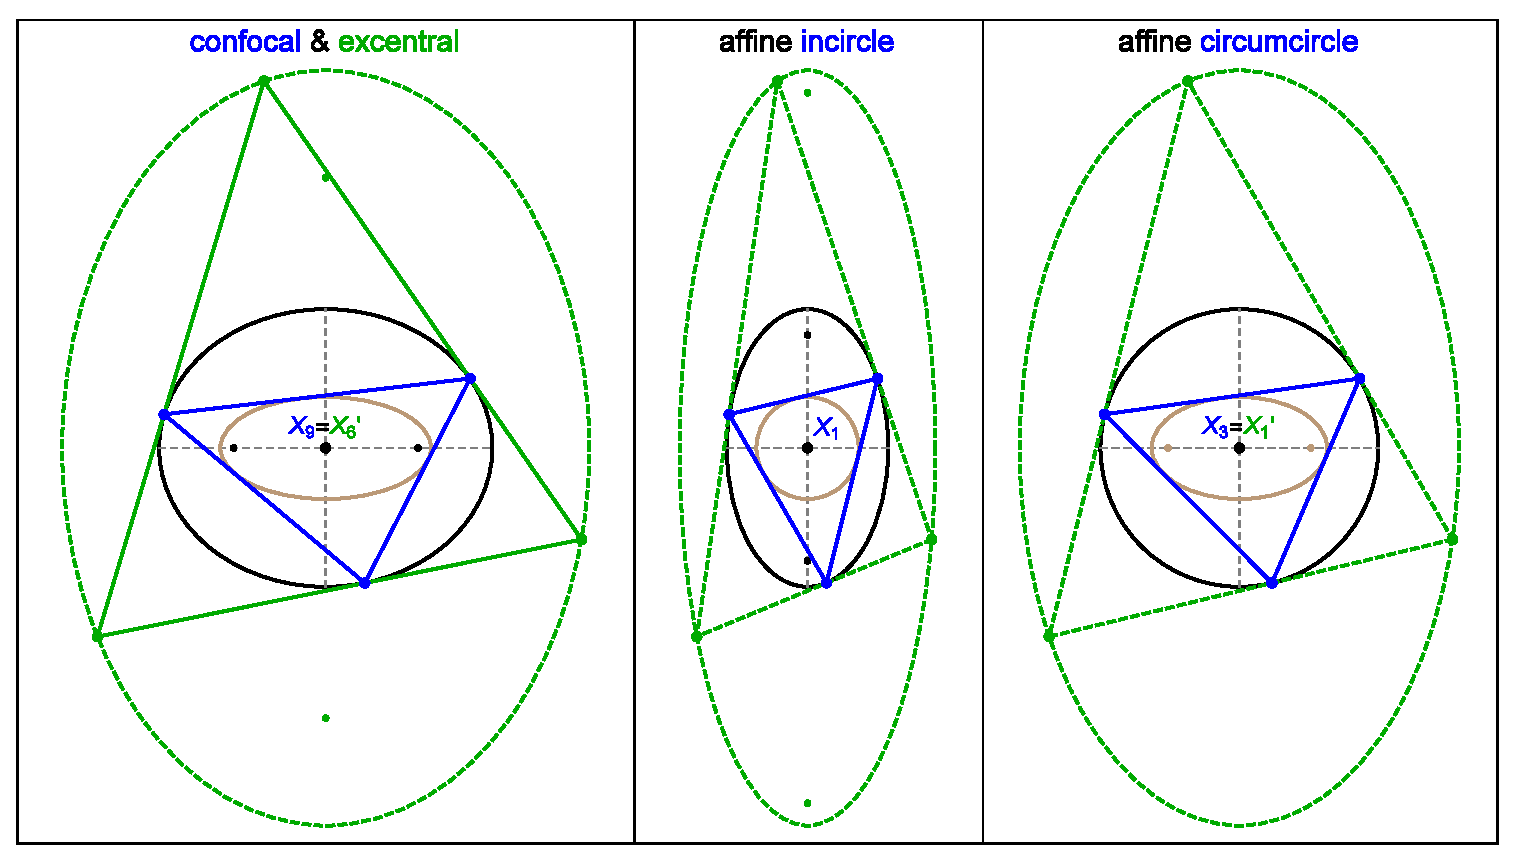
\includegraphics[width=\textwidth]{pics_03_110_n3_affine.eps}
    \caption{\textbf{Left:} billiard 3-periodic (blue) and its excentral triangle (green). The former conserves the sum of its cosines. The latter is inscribed in an ellipse (dashed green) and conserves the product of its cosines. \textbf{Middle:} Affine image of confocal family which sends caustic (brown) to a circle. This family also conserves the sum of cosines, equal to that conserved by its confocal pre-image. \textbf{Right:} Affine image of confocal family which sends billiard ellipse (black) to a circle. This family also conserves the product of cosines, equal to that conserved by the excentral family of its pre-image. \href{https://youtu.be/HjBZdrR3Azs}{Video}}
    \label{fig:03-n3-affine}
\end{figure}

\subsection{Excentral Family}

This is the Ponceletian family of excentral triangles to billiard 3-periodics. If the axes of its caustic are $a,b$, this family is inscribed in an ellipse with $a',b'$ given in \cref{thm:03-incenter-excenter}; see \cref{fig:03-n3-affine}(left).

The symmedian point $X_6$ of the excentral triangle coincides with the mittenpunkt of its reference, see \cite[X(6)]{etc}. Therefore:

\begin{corollary}
Over excentral 3-periodics, the symmedian point $X_6$ of the excentral family is stationary.
\end{corollary}

Recall that in \cref{cor:03-rOvR} two other notable invariants are mentioned: product of internal angle cosines, and ratio of its area by billiard 3-periodics.

\begin{corollary}
The invariant product of cosines of excentral 3-periodics is a quarter of the quantity in \cref{cor:03-rOvR}. Furthermore the area ratio of billiard 3-periodics by excentrals is half the quantity in \cref{cor:03-rOvR}.
\end{corollary}

Let $s_i'$ denote the variable sidelengths of the excentral family, $i=1,2,3$. Here is an additional curious invariant:

\begin{proposition}
Over the excentral family, the sum squared sidelines divided by the product of sidelines is constant. Furthermore it is equal to Joachimsthal's constant $J$ of its parent 3-periodic billiard family. Explicitly:

\[ \frac{\sum{(s_i')^2}}{\prod{s_i'}}=\frac{\sqrt{2\delta-a^2-b^2}}{c^2}={J} \]
\end{proposition}

\begin{proof}
Derive explicit expressions for excentral sidelengths and arrive at claim via CAS simplification.
\end{proof}

Referring to \cref{fig:03-cos-circle}, the {\em cosine circle} of a triangle is defined in \cite[Cosine Circle]{mw} as being centered on the symmedian point $X_6$ and containing the 6 intersections of lines through $X_6$ parallel to the sides of the orthic triangle. Its radius $r^*$ is given by the product of sidelengths divided by the sum of their squares.

\begin{corollary}
The cosine circle of the excentral family is stationary with radius $r^*=1/J$.
\end{corollary}

\begin{figure}
    \centering
    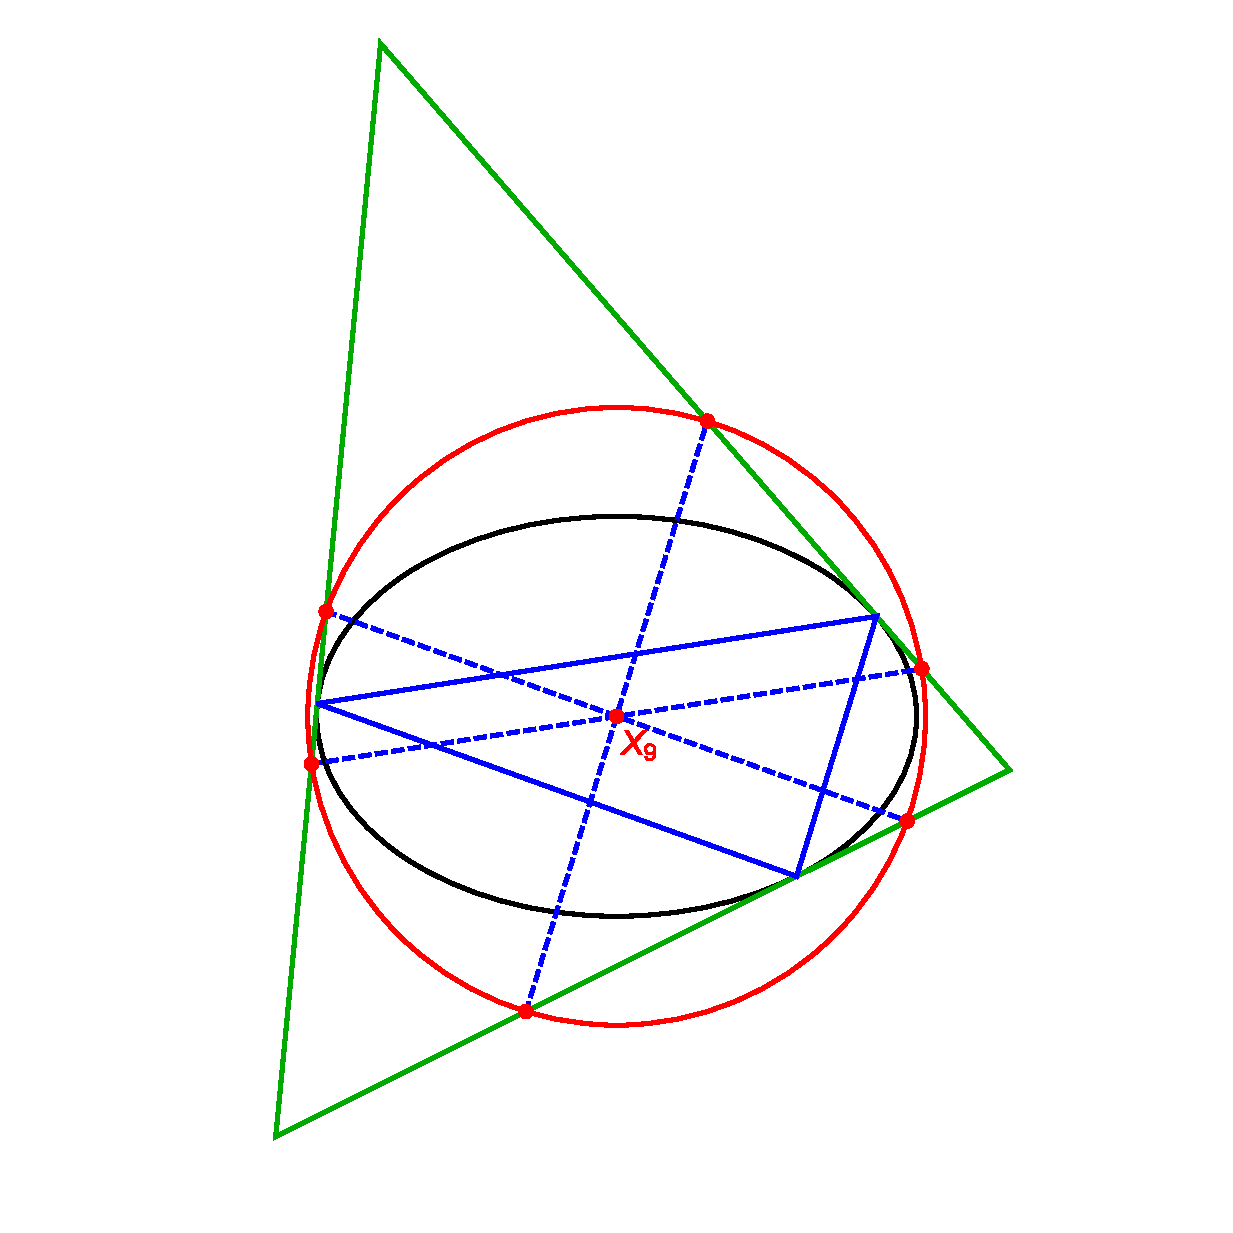
\includegraphics[width=.6\textwidth]{pics_03_130_exc_cosine_circle.eps}
    \caption{The cosine circle (red) of the excentral family (green) is stationary. It contains the 6 intersections of lines (dashed blue) through the common center (family's $X_6$ and billiard periodics' $X_9$) which are parallel to their orthic, i.e., sidelines of billiard 3 periodics. \href{https://youtu.be/CrOSI8d8qDc}{Video}}
    \label{fig:03-cos-circle}
\end{figure}

  
\subsection{Incircle Family}
The incircle family, shown in \cref{fig:03-n3-affine}(middle), is the Poncelet family in a CAP pair for which the caustic is a circle (let $r$ denote its radius). It follows immediately that the family's incenter $X_1$ is stationary. Let $a_e,b_e$ be the axes of the ellipse the family is inscribed in. Cayley yields $r=a_c=b_c=(a_e b_e)/(a_e+b_e)$. 

\begin{figure}
    \centering
    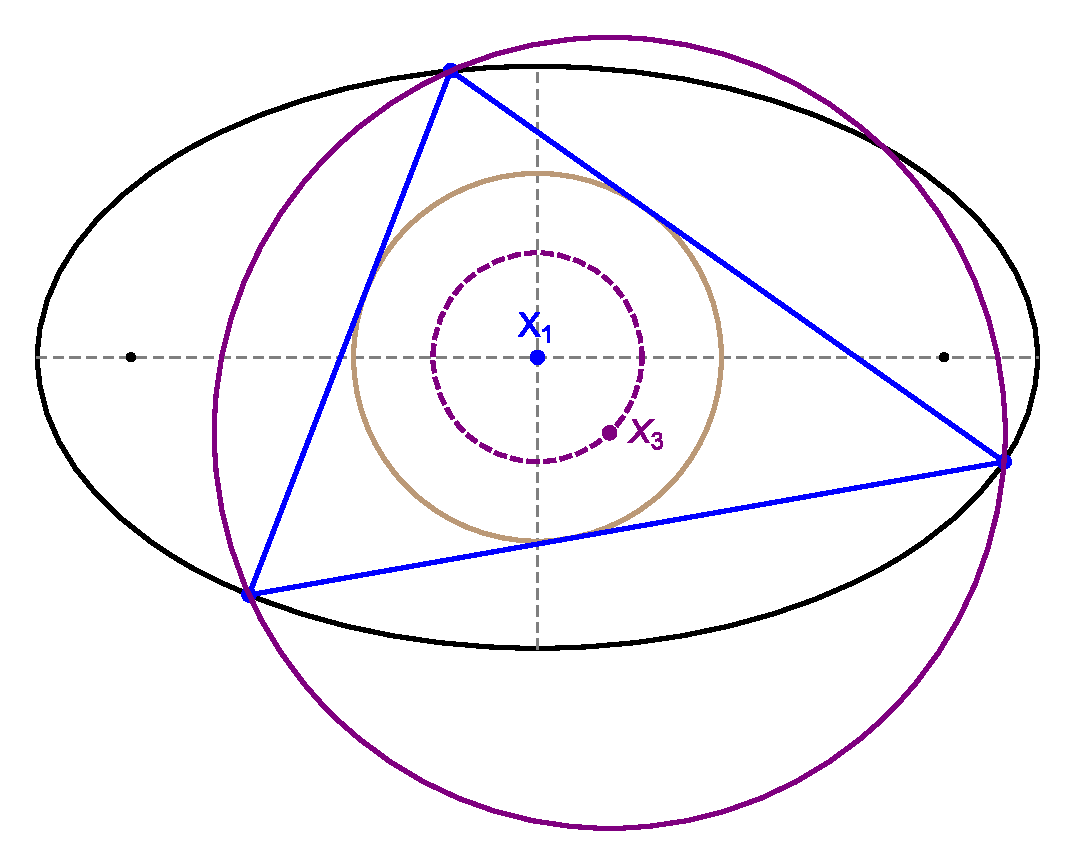
\includegraphics[width=.7\textwidth]{pics_03_160_incircle_circum.eps}
    \caption{A 3-periodic (blue) in the incircle family, and its fixed-radius circumcircle (purple). The locus of the circumcenter $X_3$ is a concentric circle (dashed purple). \href{https://bit.ly/3thddWK}{Live}}
    \label{fig:03-incircle-circum}
\end{figure}

As shown in \cref{fig:03-incircle-circum}:

\begin{proposition}
The incircle family has invariant circumradius given by $R=(a_e+b_e)/2$. Furthermore, the locus of its circumcenter $X_3$ is a circle of radius $d=R-b_e=a_e-R$ centered on the common center $O=X_1$.
\label{prop:n3-incircle-R}
\end{proposition}

\begin{proof}
Let $P_1=(x_1,y_1)$ be a first vertex of the incircle family. Using an explicit parametrization for $P_2$ and $P_3$, obtain via CAS the following coordinates for the moving circumcenter $X_3$:

{\scriptsize
\[
X_3=\frac{a_e-b_e}{2}\left[ - \,{\frac {x_1\, \left( -x_1^{2}
			\left( a_e+b_e \right) ^{2}+{a_e}^{2} b_e \left( 2\,a_e+b_e \right)  \right) }{ a_e
			\left(  \left( {a_e}^{2}-{b_e}^{2} \right) x_1^{2}+{a_e}^{2}{b_e}^{2}
			\right) }}
	 ,  {\frac { y_1\left( x_1^{2} \left( a_e+b_e
	 		\right) ^{2}-{a_e}^{2}{b_e}^{2} \right)}{b_e \left( {a_e}^{2}x_1^2+{b_e}^{2} \left( {a_e}^{2}-x_1^{2} \right)  \right) }}
	   \right]
 \]
 }

And circumradius $R=|P_1-X_3|=(a_e+b_e)/2$. Also obtain that the locus of $X_3$ is a circle concentric with the incircle and of radius $(a_e-b_e)/2$.
\end{proof}

Referring to \cref{eqn:03-sum-cos}: 

\begin{corollary}
The incircle family conserves its sum of cosines given by:
\[ \sum{\cos\theta_i}=1+\frac{r}{R}=\frac{{a_e}^2+4 {a_e}
   {b_e}+{b_e}^2}{({a_e}+{b_e})^2}\]
\label{cor:03-n3-inc-cos-sum}
\end{corollary}

\noindent \textbf{Affine image:} As \cref{fig:03-n3-affine}(middle) depicts, the incircle family can also be obtained from an affine image of billiard 3-periodics which sends the confocal caustic to a circle. As before, let $a,b$ be the semi-axes of its billiard ellipse pre-image.

\begin{lemma}
The confocal family is sent to the incircle family by scaling it along the major axis by an amount $s$ given by:

\[ s=\frac{b (\delta-c^2)}{a^3} \]

%\[ \lambda =\frac{(2a-r)\cdot r^3}{(a^2-r^2)\cdot (a-r)^2} \]
\label{lem:03-incircle-affine}
\end{lemma}

\begin{proof}
The scaled family will be inscribed in an ellipse with semi-axes $a_e = s a$, and $b_e =b$. Its caustic will be the circle $r=b_c$, where $b_c={b\left({a}^{2}-\delta\right)}/{c^2}$ is the confocal caustic minor axis given in \cref{prop:03-n3-caustic}. The Cayley condition for the incircle family imposes that $r=b_c=(a_e b_e)/(a_e + b_e)$, i.e., the result follows from solving $b_c = (s a b)/(s a + b)$ for $s$.

%The claim is obtained by imposing %$a_c^2-b_c^2=(s a)^2-b^2$ and solving %for $s^2$.
\end{proof}

\noindent Surprisingly:

\begin{proposition}
The sum of cosines conserved by the incircle family is identical to that conserved by billiard 3-periodics which are its affine pre-image.
\label{prop:03-incircle-same-sum-cos}
\end{proposition}

\begin{proof}
Let $s$ be the scaling along the major axis in \cref{lem:03-incircle-affine}. Plug $a_e=s a$ and $b_e=b$ into  \cref{cor:03-n3-inc-cos-sum}, subtract one (to obtain $r/R$ for the incircle family) and verify it yields the expression in \cref{thm:03-confocal-rovR}.
\end{proof}

\subsection{Circumcircle Family}

The circumcircle family, shown in \cref{fig:03-n3-affine}(right), is the Poncelet family in a CAP pair for which the outer ellipse is a circle (let $R$ denote its radius). It follows immediately that the family's circumcenter $X_3$ is stationary. Let $a',b'$ be the axes of its inellipse and $s_i$ the sidelengths. Cayley imposes $a'+b'=R$.

\begin{lemma}
Poncelet triangles in the circumcircle family are always acute.
\label{lem:03-circum-acute}
\end{lemma}

\begin{proof}
Since the stationary circumcenter $X_3$ is interior to the caustic caustic, it will be interior to circumcircle family triangles, and the result follows.
\end{proof}

\begin{proposition}
The circumcircle family conserves the sum of squared sidelengths. This is given by:

\[ \sum_{i=1}^3 s_i^2=4(a' + 2 b')(2 a' + b') \]
\end{proposition}

\begin{proof}
\textcolor{red}{ronaldo}
CAS-assisted simplification from vertex parametrization.
\end{proof}

\begin{proposition}
The circumcircle family conserves the product of its internal angle cosines. This is given by:
\[ \prod_{i=1}^3{\cos\theta_i}=\frac{a' b'}{2(a'+b')^2}=\frac{a' b'}{2 R^2}\]
\label{prop:03-circum-cos-prod}
\end{proposition}

\begin{proof}
CAS-assisted simplification from vertex parametrization.
\end{proof}

Recall the orthic triangle has vertices at the feet a triangle's altitudes. Let $R_h$ denote its circumradius. In , see \cite[Orthic Triangle, Eqn 7]{mw}, one finds the relation $R_h=R/2$. Therefore $R_h$ is invariant over the circumcircle family. Let $r_h$ denote the orthic's inradius. Referring to \cref{fig:03-circum-orthic}:

%Referring to Figure~\ref{fig:II-poristic} (left):

\begin{proposition}
Over the circumcircle family  $r_h$ is invariant and  given by $r_h=a' b'/(a'+b')$. 
\label{prop:03-circumcircle-rh}
\end{proposition}

\begin{proof}
In \cite[Orthic Triangle, Eqn. 5]{mw} one finds the relation  $r_h=2 R \prod_{i=1}^3{\cos\theta_i}$. Recalling $R=a'+b'$, substitution into \cref{prop:03-circum-cos-prod} yields the claim.
\end{proof}

\begin{figure}
    \centering
    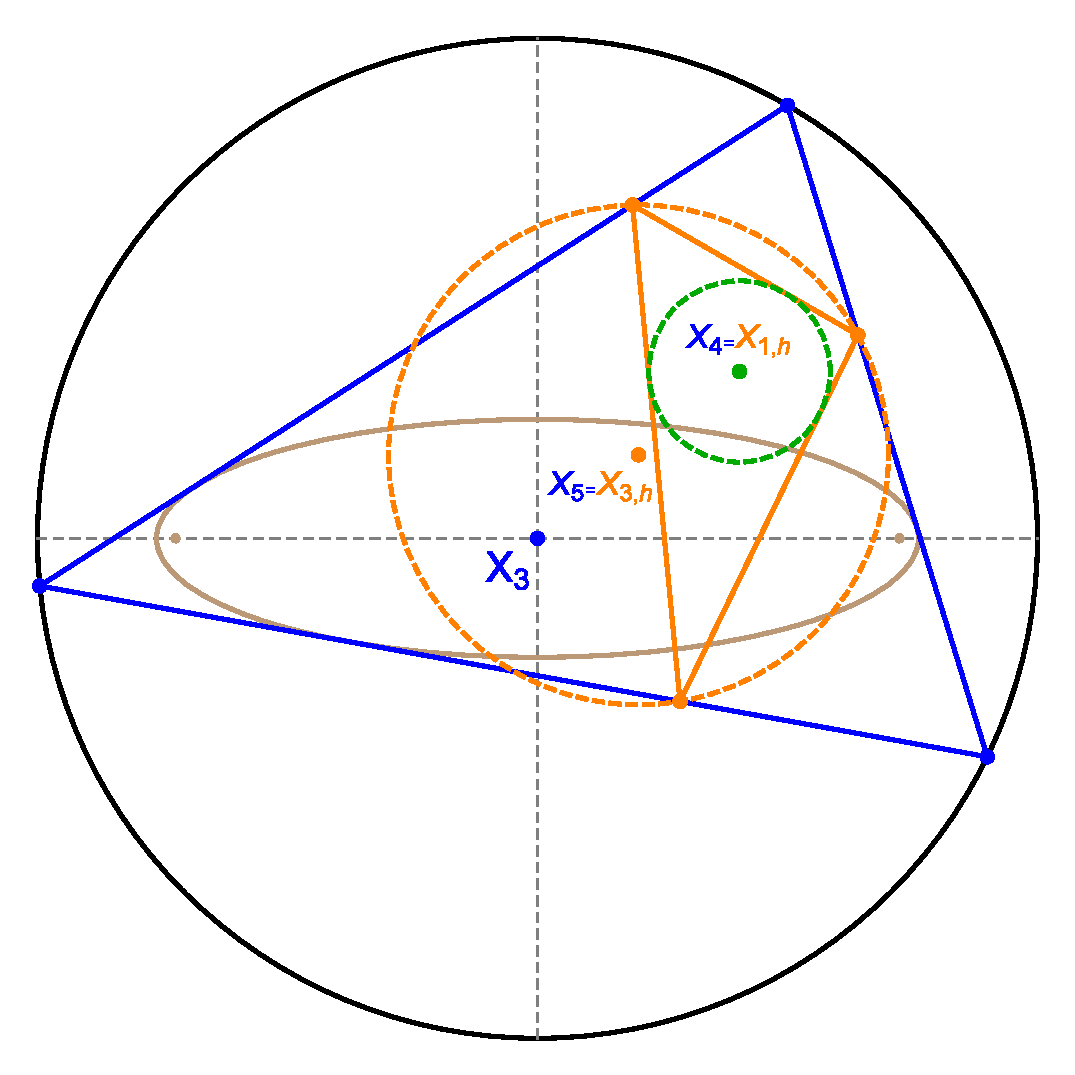
\includegraphics[width=.7\textwidth]{pics_03_140_circum_orthic.eps}
    \caption{A circumcircle family 3-periodic (blue) and its orthic triangle (orange). Over the family the orthic's circumcircle (dashed orange) and incircle (dashed green) have invariant radii. Also shown are their centers $X_{3,h}$ and $X_{1,h}$ which, for any reference triangle, correspond the nine-point center $X_5$ and orthocenter $X_1$. \href{https://youtu.be/wUu2iMesv3U}{Video}, \href{https://bit.ly/2PHJZma}{Live}}
    \label{fig:03-circum-orthic}
\end{figure}


Referring to  \cref{fig:03-circum-orthic}, it can be shown (see \cref{ex:03-circum-x5-locus}):

\begin{lemma}
Over the circumcircle family, the locus of the orthic circumcenter (i.e., the 9-point center $X_5$ of the family) is a circle concentric with the pair.
\label{lem:03-circum-x5-locus}
\end{lemma}

%Below we analyze a Poncelet family with fixed incircle and non-concentric fixed circumcircle, known as the ``poristic'' family. The previous result implies that the orthics derived from the circumcircle family can be regarded as a rigidly moving poristic family.

\noindent \textbf{Affine image:} As \cref{fig:03-n3-affine}(right) depicts, the circumcircle family can also be obtained from an affine image of billiard 3-periodics which sends the billiard ellipse with semi-axes $a,b$ to a circle with radius $R=b$. Therefore billiard 3-periodics are sent to the circumcircle family by scaling it along the major axis by an amount $s'={b/a}$. Therefore \cref{prop:03-n3-caustic} implies:

\begin{lemma}
The caustic semi-axes $a',b'$ of the circumcircle family which is the $s'$-affine image of the confocal family are given by:

\[ a'=\frac{b}{a}{a_c}=\frac{b(\delta-b^2)}{c^2},\;\;\;b'=b_c=\frac{b(a^2-\delta)}{c^2} \]
\label{lem:03-circumcircle-affine}
\end{lemma}

\noindent Note that the $s'$-affine image of billiard excentrals becomes a Poncelet family with fixed incircle; see \cref{fig:03-n3-affine}(right, dashed green triangles). We have seen above such a family conserves its sum of cosines. Suprisingly, the following invariant ``role reversal'' takes place:

\begin{proposition}
The sum of cosines conserved by billiard 3-periodics is the same as the one conserved by the $s'$-affine image of billiard excentrals. Furthermore product of cosines conserved by billiard excentrals is the same as the one conserved by the $s'$-affine image of billiard 3-periodics (circumcircle family). Furthermore, \label{prop:03-n3-role-reversal}
\end{proposition}

\begin{proof}
For the first statement it suffices to show that the $s'$-affine image of billiard excentrals has sides parallel to those of the $s$-image of billiard 3-periodics, i.e., the incircle family and use \cref{prop:03-incircle-same-sum-cos}.
\textcolor{red}{ronaldo consegue seguir}
\end{proof}

\subsection{Homothetic Family}
 
\begin{figure}
    \centering
    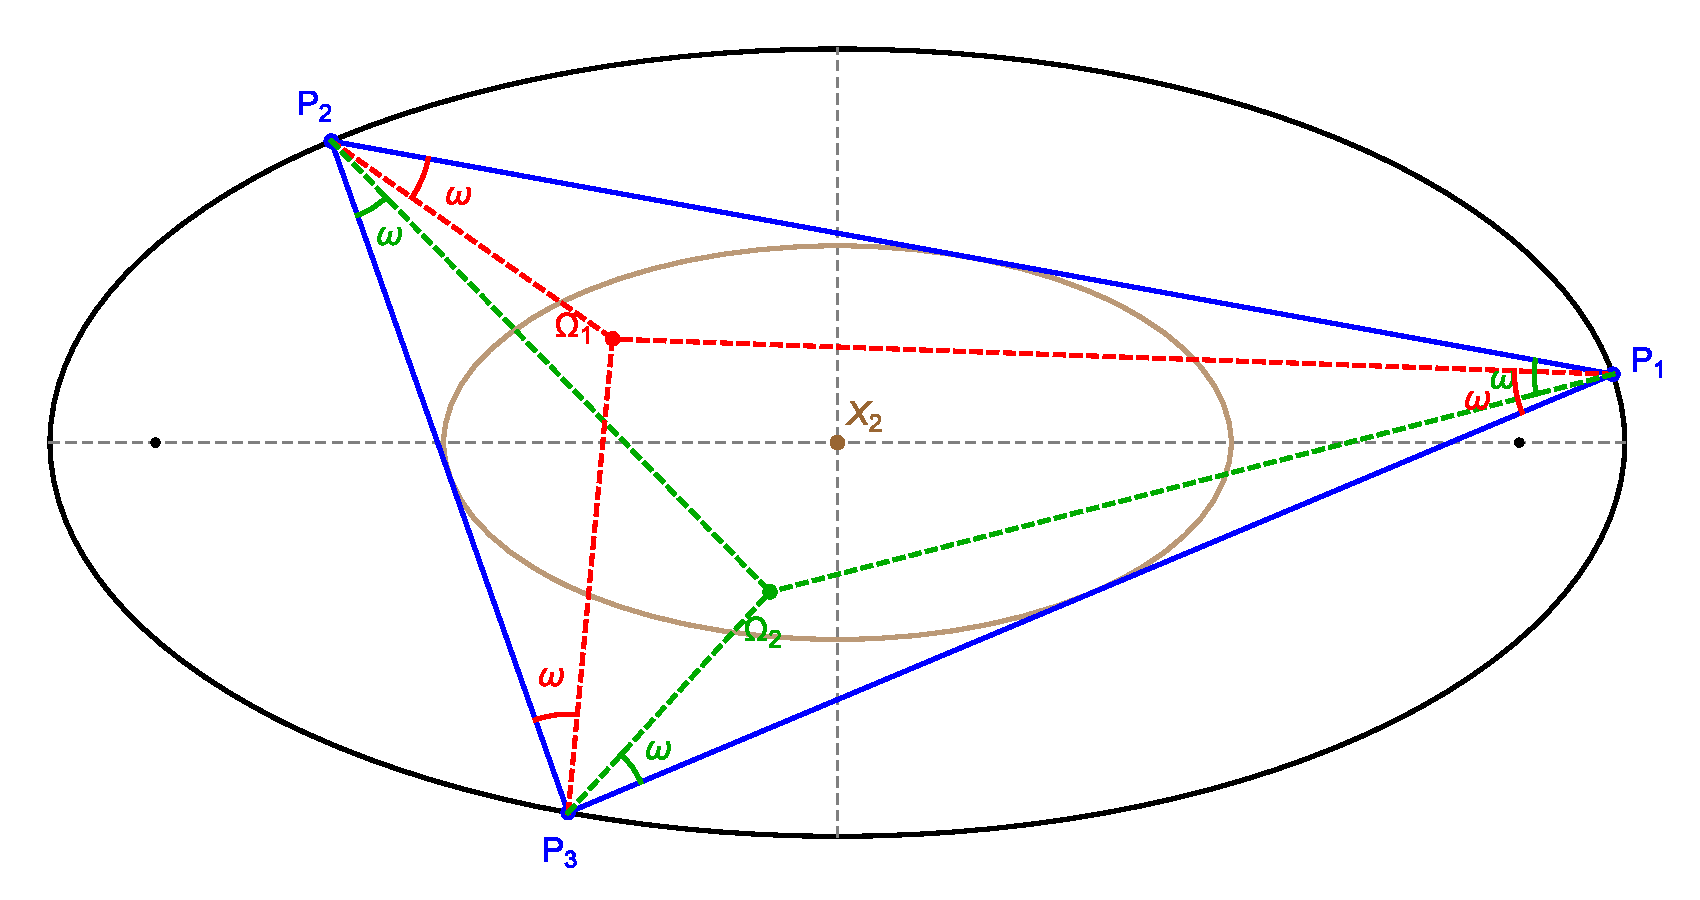
\includegraphics[width=\textwidth]{pics_03_150_n3_homothetic.eps}
    \caption{A 3-periodic (blue) interscribed between two homothetic ellipses (black, brown). Since this family is an affine image of one of equilaterals interscribed between two concentric circles, (i) the barycenter $X_2$ is stationary at the common center, and (ii) the area is conserved. Also conserved is (iii) the sum of squared sidelengths. (ii) and (iii) imply the Brocard angle $\omega$ is invariant. Also shown are the two (moving) the Brocard points $\Omega_1$ and $\Omega_2$. \href{https://youtu.be/2fvGd8wioZY}{Video}, \href{https://bit.ly/3aYnrVM}{Live}}
    \label{fig:03-homoth-brocard}
\end{figure}

The homothetic family, shown in \cref{fig:03-homoth-brocard}, is the Poncelet family in a CAP pair for which the outer and inner ellipse are homothetic to each other, i.e., $a_e = k a'$ and $b_e = k b'$, where $a_e,b_e$ and $a',b'$ are outer and inner ellipse semi-axes, respectively. Cayley imposes a homothecy ratio $k=1/2$.

\begin{proposition}
The barycenter $X_2$ is stationary at the common center and area $A$ is invariant and given by:
\[A= \frac{3\sqrt{3}}{4} a_e b_e \]
\end{proposition}

\begin{proof}
Consider an affine transformation that sends both outer and inner ellipse to a unit circle, e.g., by scaling the system along the major (resp. minor) axis by $1/a_e$ (resp. $1/b_e$). Uniquely amongst all triangle centers, the barycenter $X_2$ is invariant under affine transformations. By symmetry of the equilateral centroid, it will be identified with the center of the homothetic pair. Affine transformations preserve area ratios, so $A$ will be the the area of an equilateral triangle inscribed in a unit circle scaled by the inverse Jacobian $a_e b_e$. This completes the proof.
\end{proof}

Curiously, the homothetic family shares the following invariant with the circumcircle family:

\begin{proposition}
Over the homothetic family, the sum of squared sidelengths $s_i^2$ is invariant and given by:
	
\[ \sum_{i=1}^3 s_i^2=\frac{9}{2} \left({a_e}^{2}+{b_e}^{2}\right) \]
\end{proposition}

\begin{proof}
CAS-simplification from vertex parametrization.
\end{proof}

Referring to \cref{fig:03-homoth-brocard}, recall the definition of a triangle's Brocard angle $\omega$, given in \cite[Brocard Angle]{mw}: sidelines $P_i P_{i+1}$ rotated about $P_i$ by some angle $\alpha$ will only concur (at the first Brocard point $\Omega_1$) if $\alpha=\omega$. A second, distinct Brocard point $\Omega_2$ exists if sidelines $P_i P_{i-1}$ are rotated about $P_{i}$ by $-\omega$.

A known relation appearing in \cite[Brocard Angle, Eqn. 2]{mw} is $\cot\omega=(\sum_{i=1}^3 s_i^2)/(4 A)$. Therefore:

\begin{corollary}
Over the homothetic family, the Brocard angle $\omega$ is invariant. Its cotangent is given by:
\[ \cot\omega=\frac{\sqrt{3}}{2} \frac{{a_e}^{2}+{b_e}^{2}}{a_e b_e} \]	
\end{corollary}

\begin{proof}
Direct calculations using the explicit parametrization of homothetic vertices.
\end{proof}

\noindent Another known relation valid for any triangle is $\cot\omega=\sum\cot\theta_i$:

\begin{corollary}
The homothetic family conserves the sum of its internal angle cotangents.
\end{corollary}

\subsection{Dual Family}

\begin{figure}
    \centering
    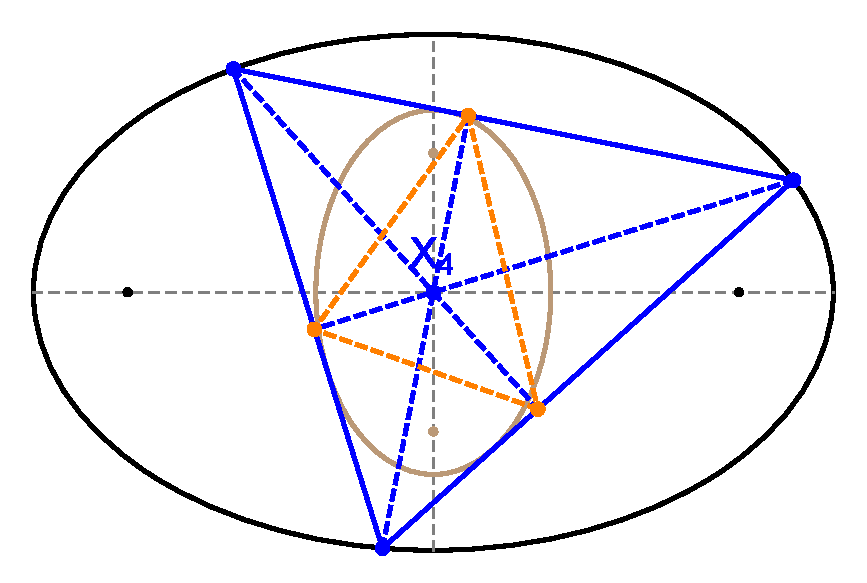
\includegraphics[width=.7\textwidth]{pics_03_120_dual_w_orthic.eps}
    \caption{A Dual family 3-periodic (blue) interscribed in a pair of ``dual'' ellipse (black, brown). Their aspect ratios are reciprocals of each other. No invariants have yet been detected for this family other than the fact that the orthocenter $X_4$ is stationary at the common center. Also shown is the orthic triangle (dashed orange) whose vertices lie at the feet of the altitudes (dashed blue). \href{https://bit.ly/337wTBS}{Live}}
    \label{fig:03-n3-dual}
\end{figure}

%\textcolor{red}{Quem e o dual: é aquele cuja caustica é anti-homotetica a externa, ou seja $a'/b'=b/a$}

The dual family, shown in \cref{fig:03-n3-dual}, is the Poncelet family in a CAP pair such that the outer and inner ellipses are ``duals'' curves of each other, i.e., tangents to one are sent to points on the other and vice-versa. For ellipses, this simply implies their aspect ratios $a_e/b_e$ and $a'/b'$ will be reciprocals of one another. Cayley yields $a'=\lambda b_e,\; b'=\lambda a_e$ and therefore $\lambda= a_e b_e/(a_e^2+b_e^2)$. Remarkably:

\begin{proposition}
The orthocenter $X_4$ of the dual family is stationary.
\end{proposition}

\begin{proof}
Follows directly from the vertex parametrization, see \cref{eq:03-n3-conc-general}.

In terms of the vertices of a triangle $A=[x_a,y_a]$, $B=[x_b,y_b]$, $C=[x_c,y_c]$ the orthocenter $X_4=[x_{4n}/A_4,y_{4n}/A_4]$ is given by the following rational functions 

\begin{align*}
    x_{4n}&=   \left(x_c-x_b\right) x_a\,y_a+ \left( 
 x_b\,y_b-x_c\,y_c \right) x_a+ \left( y_c-y_b \right) y_a^2+ \left( y_b^2-{y_c}^{2} \right) y_a\\
&+  x_cx_b\left( \,y_c- \,y_b)
 \right) +y_by_c( y_c-y_b) \\
 \\
 y_{4n}&=  \left(x_b-x_c\right) x_a^2+ \left( y_b-y_c \right) x_a\,y_a+ \left( x_c^2-x_b^2\right) x_a+ \left( -x_b\,y_b+x_c\,y_c \right) y_a\\
 &+x_b  x_c(x_b- \,x_c)+ y_b\,y_c(x_b-x_c) \\
 %
A_4&= \left(y_b-y_c \right) x_a+ \left( -x_b+x_c\right) y_a+x_b\,y_c-x_c\,y_b
\end{align*}

Therefore, using  the vertex parametrization, see \cref{eq:03-n3-conc-general}, and CAS the result follows by direct computations.
\end{proof}

Despite much searching, no invariant quantities have yet been found for this family.

\begin{table}
\centering
\begin{tabular}{|r|c|c|l|}
\hline
Family & Fixed & Conserves & Notes \\
\hline
Confocal & $X_9$ & $L$, $J$, $r/R$, $\sum\cos\theta_i$ & i.e., billiard 3-periodics \\
\hline
Incircle & $X_1$ & $R$, $\sum\cos\theta_i$ & \makecell[lc]{sum of cosines same as\\confocal affine pre-image} \\
\hline
Circumcircle & $X_3$ & \makecell[cc]{$\sum{s_i^2}$, $\prod\cos\theta_i$,\\$r_h$,$R_h$} & \makecell[lc]{product of cosines same as\\excentrals' in confocal affine\\pre-image} \\
\hline
\makecell[rc]{Confocal\\Excentrals} & $X_6$ & \makecell[cc]{$A'/A$, $\prod\cos\theta_i'$,\\$\sum{(s_i')^2}/\prod{s_i'}$} & \makecell[lc]{primed quantities refer to those\\of the excentral family}  \\
\hline
Homothetic & $X_2$ & $A$, $\sum{s_i^2}$, $\omega$, $\sum\cot\theta_i$ & affine image of concentric circles  \\
\hline
Dual & $X_4$ & n/a &  \\
\hline
\end{tabular}
\caption{Summary of fixed points and (known) conserved quantites for the CAP families mentioned in this section.}
\label{tab:n3-conc-families}
\end{table}

\subsection{Vertex parametrization for any CAP pair}

Consider a general pair of CAP ellipses denoted $\E$ and $\E_c$. We will derive a generic parametrization for the vertices of 3-periodics in such a pair. A first calculation will be helpful. Referring to \cref{fig:ell-ints}(left), the following are coordinates for the intersections $P_2$ and $P_3$ on $\E$ of the two tangents to $\E_c$ seen from a point $P_1=[x_1,y_1]$ also on $\E$:

\begin{figure}
    \centering
    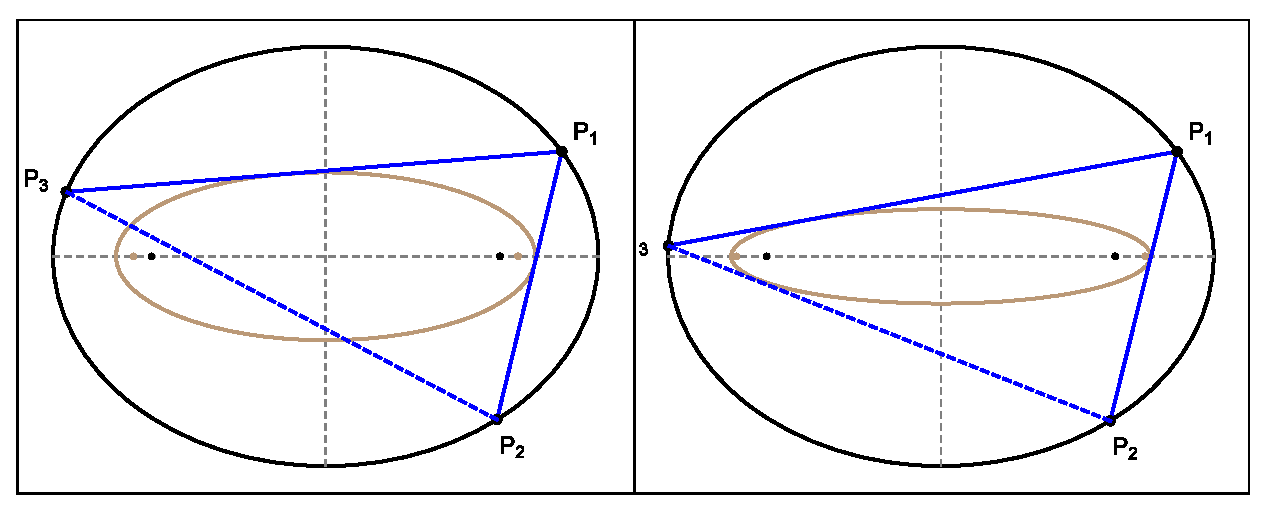
\includegraphics[width=\textwidth]{pics_03_070_ell_ints.eps}
    \caption{\textbf{Left:} Two CAP ellipses (black and brown), and a point $P_1$ on the outer one. The lines thru $P_1$ tangent to the inner ellipse intersect the outer one at $P_2$ and $P_3$. Notice that $P_2 P_3$ cut thru the inner ellipse, i.e., the pair of ellipses does not satisfy Cayley's conditions. \textbf{Right:} the minor axis of the inner ellipse has been scaled such that $P_1 P_2 P_3$ is now a Poncelet triangle.}
    \label{fig:ell-ints}
\end{figure}

\textcolor{red}{ronaldo reduzi a notação, pode checar? que tal minúsculas para escalares, maiúsculas para pontos; exceção historica: L e J}
\begin{align}
    P_2& =[x_2,y_2]=\frac{1}{k_2}\left[\frac{u_1 x_1 + u_2 y_1}{b} ,  \frac{w_1 x_1 + w_2 y_1}{a} \right] \label{eq:03-n3-conc-general} \\
    P_3&=[x_3,y_3]=\frac{1}{k_2}\left[\frac{w_1 x_1 - w_2 y_1}{b},\frac{w_1 x_1 - w_2 y_1}{a}\right] \nonumber
\end{align}
where:
\begin{align*}
    u_1 &=b\left(a^4  b_c^4 -(a^2 -  a_c^2)^2 b^4 \right) \\
    u_2 &= 2 a k_1 \left( (a^2 + a_c^2)b^2 - b_c^2 a^2\right) \\
    k_1&=\sqrt{ b^2  b_c^2 (a^2 -  a_c^2)  x_1^2 +  a_c^2 a^2(b^2 -  b_c^2)  y_1^2}\\
    k_2 &=\left(\frac{a^2 (b^2 +  b_c^2) - a_c^2 b^2 }{a}x_1\right)^2+ \left(\frac{a^2 (b^2 -  b_c^2) + a_c^2b^2 }{b} y_1\right)^2\\
    w_1&=2 b k_1\left( (b^2 +  b_c^2) a^2 - a_c^2 b^2\right) \\
    w_2&= a\left(a_c^4b^4-a^4(b^2-b_c^2)^2\right)
     %=-a (a^2( b^2 -    b_c^2) -  a_c^2 %b^2) (a^2 (b^2 -   b_c^2) +  a_c^2 b^2)
\end{align*}

 
\section{Some Non-Concentric Families}
\label{sec:03-non-conc}
 Here we introduce a few Poncelet triangle families interscribed in non-concentric, axis-parallel (NCAP) ellipse pairs. In some of the families below, at least one of the ellipses is a circle, so perhaps ``co-axial'' could also be employed.

\section{Poristic Family (Bicentric Triangles)}

\begin{figure}
    \centering
    %\includegraphics[width=\textwidth]{pics/0010x_obtuse_poristics.eps}
    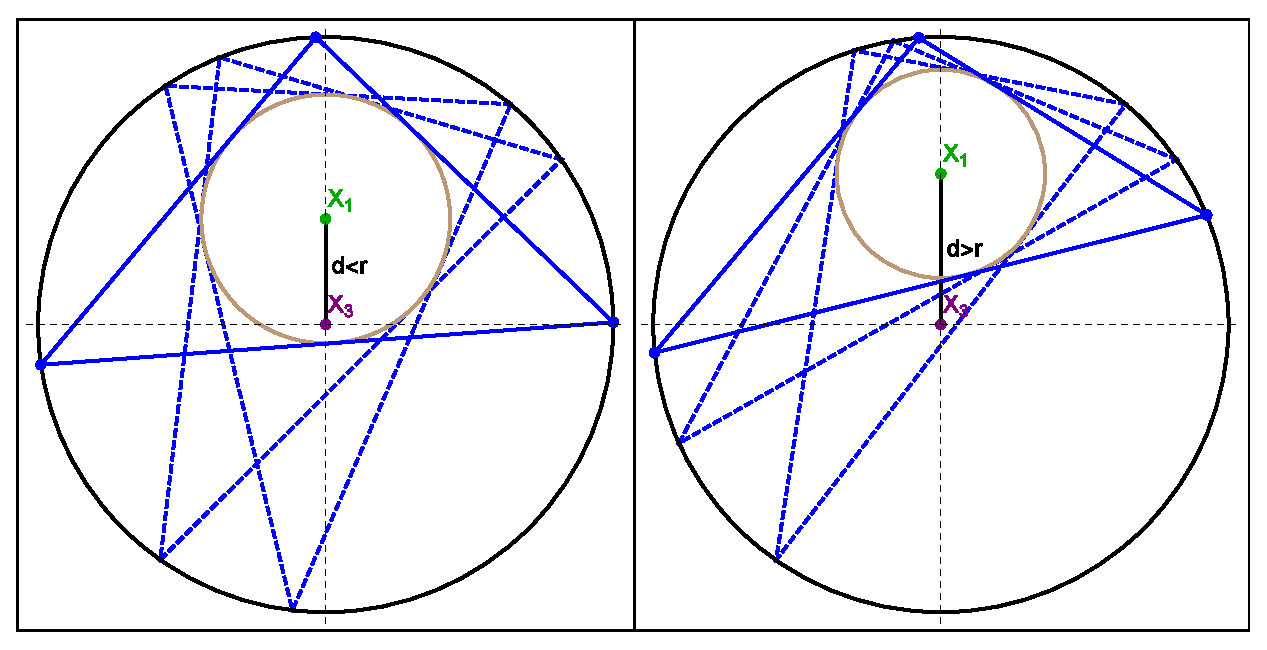
\includegraphics[width=\textwidth]{
    pics_03_180_obtuse_poristics.eps}
    \caption{Poristic Triangle family (blue): fixed incircle (green) and circumcircle (purple). \textbf{Left}: a few poristic triangles (blue and dashed blue) in a pair of circles such that $d<r$, i.e.,  all poristic triangles are acute. \textbf{Right}: the same but with $d>r$; since $X_3$ can be either interior or exterior to the family, both acute and obtuse triangles will be present. \href{https://bit.ly/3bg19iD}{Live}}
    \label{fig:03-poristic obtuse}
\end{figure}

Poristic triangles, shown in \cref{fig:03-poristic obtuse}, are the simplest case of Poncelet's porism: a 1d family of triangles with fixed incircle and circumcircle. They are they $N=3$ case of the bicentric family covered in \cref{chap:06-bicentric}.

First described by \cite{chapple1746-poristics}, the family was later studied by both Euler and Poncelet. The so-called Euler's triangle formula\footnote{Chapple had stated it in 1746, Euler in 1765, and Poncelet's porism was published in 1822; see \cite{centina15}.}, constrains the distance $d$ between incenter $X_1$ and circumcenter $X_3$ as follows:

\begin{equation}
d^2=R(R-2 r)
\label{eq:03-euler-poristic}
\end{equation}
where $r,R$ are the radii of outer and inner circle. Referring to \cref{fig:03-poristic obtuse}:

\begin{proposition}
The Poristic family will contain obtuse triangles iff $d>r$.
\end{proposition}

\begin{proof}
This stems from the fact that when $d<r$, $X_3$ is always interior to the incircle, i.e., the caustic of the Poncelet family. 
\end{proof}

In consonance with both billiard 3-periodics and the incircle family:

\begin{proposition}
The poristic family conserves the sum of its internal angle cosines.
\end{proposition}

\begin{proof}
Direct application of \cref{eqn:03-sum-cos}, noting by definition $r/R$ is constant.
\end{proof}

\begin{figure}
    \centering
    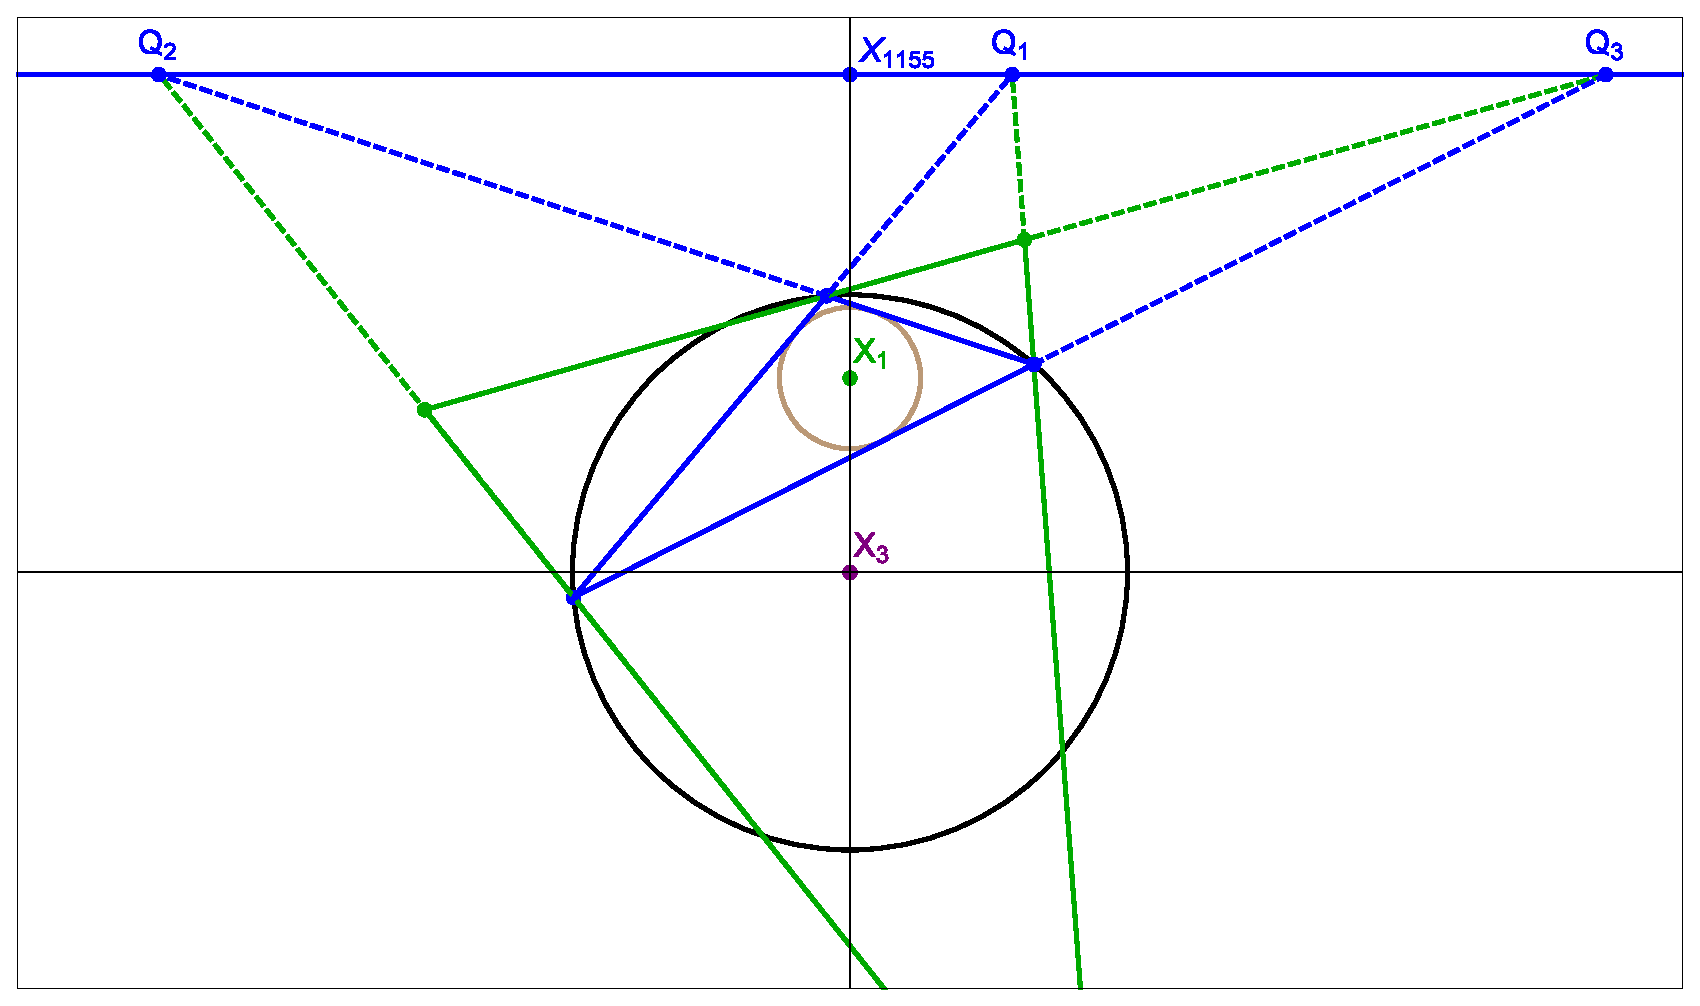
\includegraphics[width=.7\textwidth]{pics_03_220_poristic_antiorthic.eps}
    \caption{Over the poristic family, the antiorthic axis (solid blue) is stationary and perpendicular to $X_1 X_3$. \href{https://youtu.be/DS4ryndDK6Q}{Video}.}
    \label{fig:03-antiorthic}
\end{figure}

In \cite[Antiorthic axis]{mw} the anti-orthic axis is defined as containing the three intersections of a triangle's sidelines with those of the excentral triangle. As illustrated in \cref{fig:03-antiorthic}, the following was proved by \cite{weaver1927-poristic}:

\begin{proposition}
The antiorthic family is stationary over the poristic family and perpendicular to $X_1 X_3$.
\label{prop:03-antiorthic}
\end{proposition}

Let a first vertex $P_1$ of the poristic family be parametrized by $P_1(t)=R[\cos{t},\sin{t}]$.

\begin{proposition}
The perimeter $L(t)$ of poristic triangles is given by:

\begin{equation*}
L(t)=\frac {\left(3\,{R}^{2}
-4\,dR\cos t  +{d}^{2} \right)\sqrt{3\,{R}^{2}+2\,dR\cos t  -{d}^{2}}  }{R\sqrt {{R}^{2}-2\,dR
\cos t  +{d}^{2}}}\\
\end{equation*}
\end{proposition}
\begin{proof}
Follows directly computing the 3-vertices explicitly and using $L(t)=|P_1-P_2|+|P_2-P_3|+|P_3-P_1|$ and simplifying it with a CAS.  
\end{proof}

It turns out poristic triangles can be regarded as the image of billiard 3-periodics (and vice-versa) under (i) a variable similarity transform, and (ii) a polar transformation wrt to a focus-centered circle. We now proceed to prove these results, but first we will need a couple of lemmas.

In \cite[page 17]{odehnal2011-poristic}, one finds the following result, illustrated in \cref{fig:03-poristic-x9}:

\begin{figure}
    \centering
    %\includegraphics[width=.8\textwidth]{pics/0050x_poristic_cb.eps}
    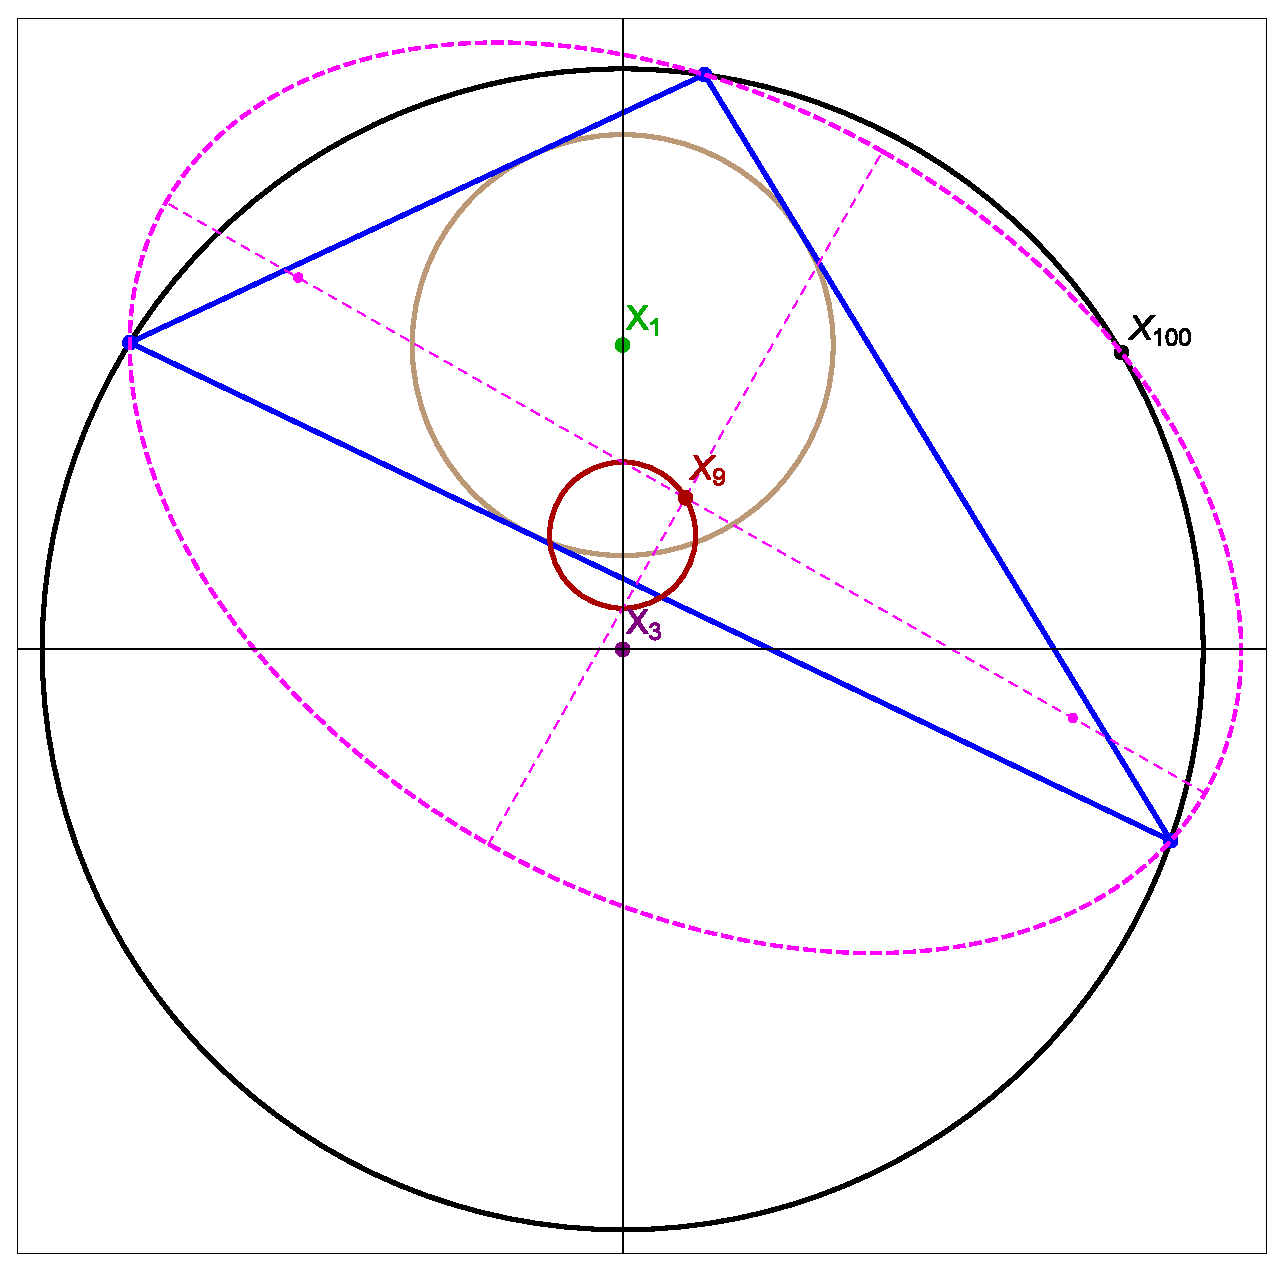
\includegraphics[width=.8\textwidth]{pics_03_190_poristic_cb.eps}
    \caption{A poristic triangles (blue) is shown along as its circumbilliard (dashed magenta) whose aspect ratio is invariant. The locus of the mittenpunkt $X_9$ is a circle (red). \href{https://youtu.be/LGgh11LMGGY}{Video}, \href{https://bit.ly/3tcGtOj}{Live}}
    \label{fig:03-poristic-x9}
\end{figure}

\begin{lemma}
Over the poristic family, the locus of the mittenpunkt $X_9$ is a circle with radius is $R{d^2}R/(9R^2-d^2)$ centered on $X_1 + (X_1 - X_3) (2 R - r)/(4 R + r)=d (3 R^2+d^2)/(9R^2-d^2)$. 
\end{lemma}

In fact we can derive $X_9(t)$ explicitly:

\begin{lemma}
{\small
\begin{align}
    X_9(t)= &\left[  \frac {d \left( 4\, d \mathbf{c}^2   
 \left( R\mathbf{c}_t-d \right) -r \left( 3\,d\mathbf{c}_t  +R \right) -{r}^{2} \right) }{ \left( 4\,R+r \right) 
 \left(d \mathbf{c}_t  -R+r \right) }
  , \, \frac {4R{d}^{2}\mathbf{s}_t  \left( R^2- \left( 2\,R\mathbf{c}_t-d \right) ^{2}  \right) }{ \left( {R}^{2}+{d
}^{2}-2\,dR\mathbf{c}_t  \right)  \left( 9\,{R}^{2}-{d}^{2}
 \right) }
    \right]
\label{eq:03-x9-poristic}
\end{align}
where $\mathbf{c}_t$ and $\mathbf{s}_t$ are shorthand for $\cos(t)$ and $\sin(t)$ respectively.
}
\end{lemma}

Let $P_i=[x_i,y_i]$ denote the vertices of billiard 3-periodics and $P_i'=[x_i',y_i']$ those of a poristic family, $i=1,2,3$.

\begin{theorem}
The $P_i'$ are an image of the $P_i$ under a variable similarity transform comprising of (i) a rigid rotation by $\theta(t)$, (ii) a rigid translation by $X_9(t)$, and (iii)  uniform scaling by $L(t)$. These are given by: 

\begin{align*}
    x_i'=&L(t)(\cos \theta(t) x_i+\sin\theta(t) y_i+x_9(t) )\\
    y_i'=&L(t)(-sin\theta(t) x_i+\cos\theta(t) y_i+y_9(t))\\
    \tan\theta(t)=& \frac{(1-\cos t)(R+d-2R\cos t)}{(2R\cos t+R-d)\sin t}
\end{align*}
\label{thm:similarity}
\end{theorem}

\begin{proof} 
CAS-assisted simplification.
\end{proof}

In \cite{reznik2021-circum} term the ``circumbilliard'' $E_9$ of a triangle the circumellipse centered on $X_9$. Let $a_9,b_9$ its semi-axes. CAS manipulation yields:

\begin{corollary}
Over the poristic family, $a_9(t)$ and $b_9(t)$ are given by:
\begin{align*}
a_9=&L(t)\frac{R\sqrt {3\,{R}^{2}+2\,dR-{d}^{2}} }{9\,{R}^{2}-{d}^{2}}\\
b_9=&  L(t)\frac{R\sqrt {R-d}}{\sqrt {3\,R+d} (3\,R-d)}\\
  c_9=&\sqrt{a_9^2-b_9^2}=L(t)\frac{2R\sqrt{dR}}{9R^2-d^2}.
\end{align*}
\end{corollary}

\begin{corollary}
The ratios $a_9(t)/L(t)$, $b_9(t)/L(t)$, and $c_9(t)/L(t)$ are invariant over the Poristic family.
\end{corollary}

\begin{corollary}
Over the poristic family, the aspect ratio of the (varying) circumbilliard is invariant and given by:

\begin{equation*}
\frac{a_9(t)}{b_9(t)}=\sqrt{\frac { \left(  R+d \right)  \left( 3R-d \right) }{ \left( R-d
 \right)  \left( 3\,R+d \right) }}
\end{equation*}
\end{corollary}

In \cite[Polar]{mw}, the {\em polar} of a point $P$ with respect to a circle $\Cm$ is defined as the line perpendicular to $O P$ which contains the inversion of $P$ wrt to $\Cm$. Dually, the pole of a line $L$ with respect to $\Cm$ is the inversion of the foot of the perpendicular dropped from $O$ onto $P$ wrt to $\Cm$.

So given a smooth curve, we can speak of its {\em polar image} with respect to a circle as the set of poles of the curve's tangents with respect to $\Cm$. 

\begin{figure}
    \centering
    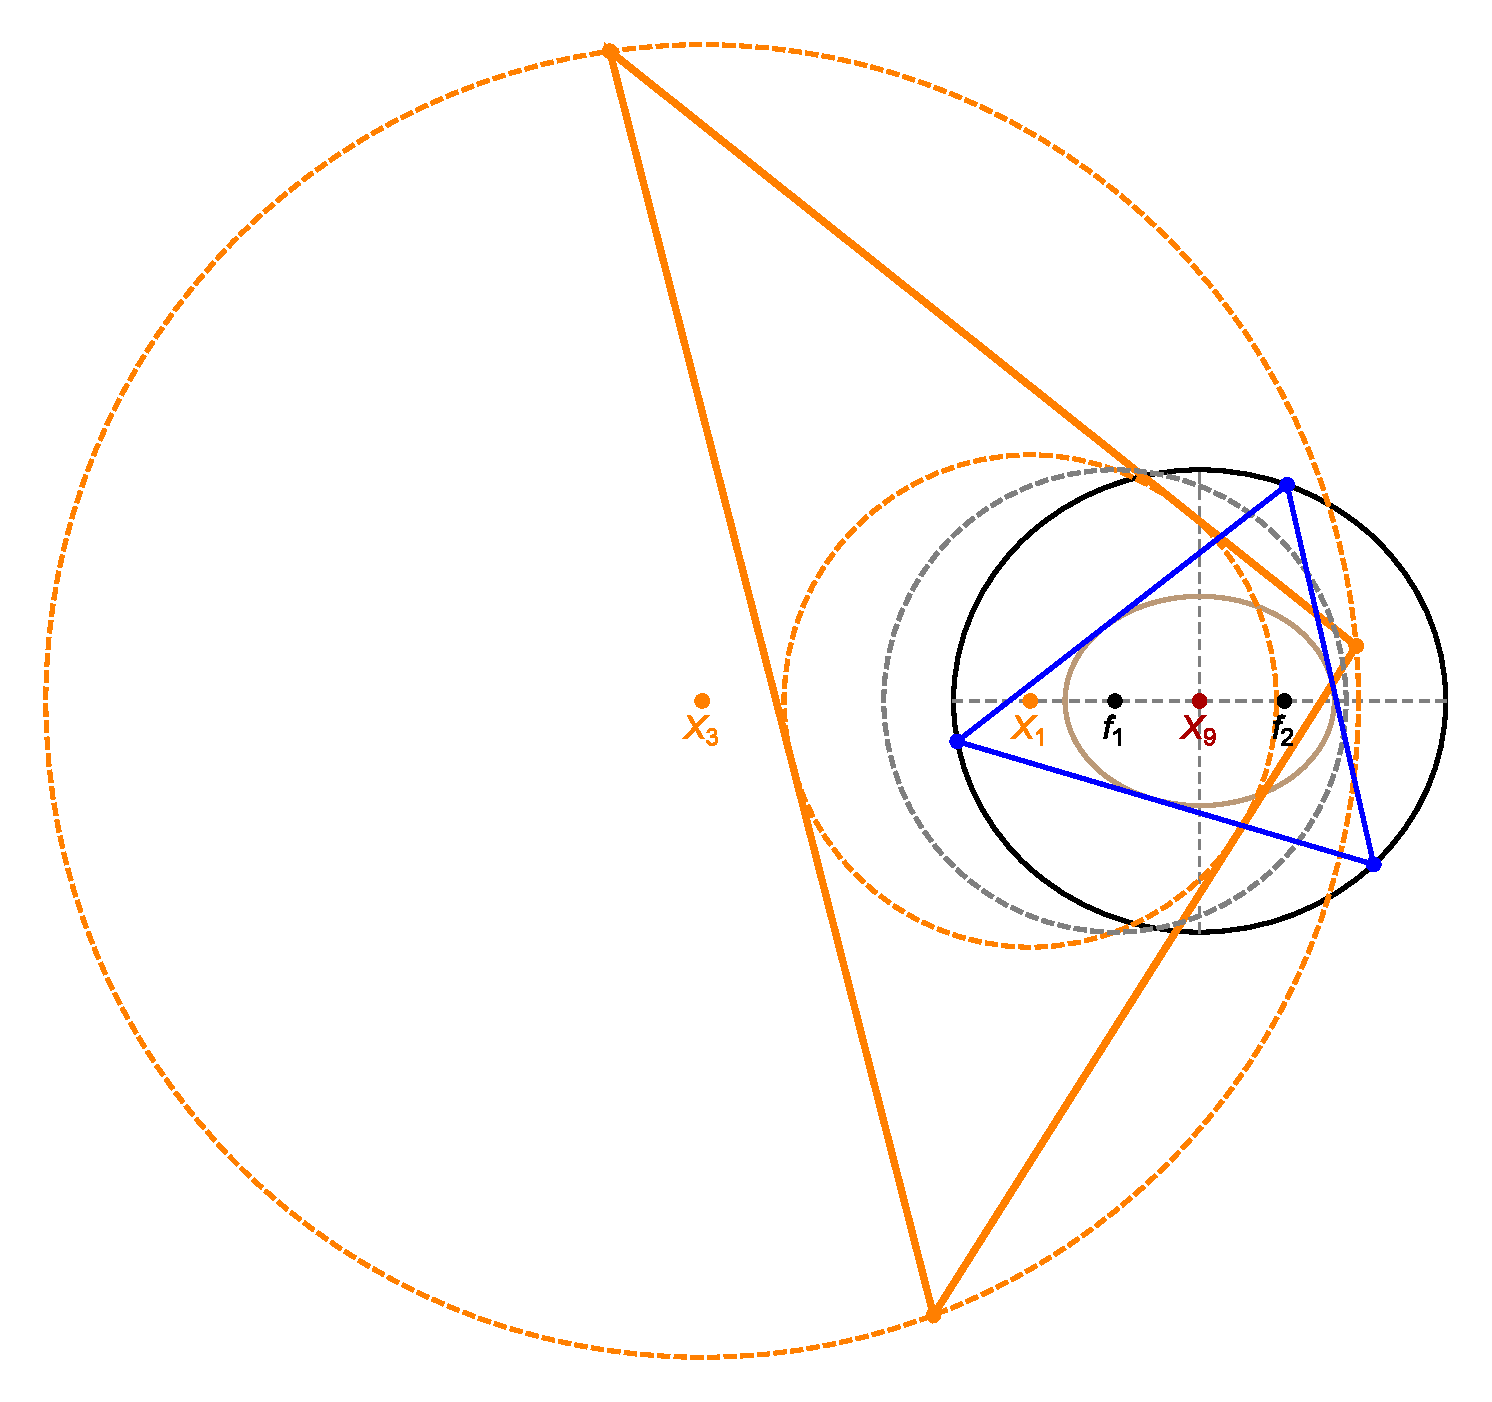
\includegraphics[width=.8\textwidth]{chap_03/pics/pics_03_200_polar_poristic.eps}
    \caption{The poristic family (orange) is the polar image of billard 3-periodics (blue) with respect to a circle (dashed gray) centered on one of the foci of the confocal pair ($f_1$ in the picture). \href{https://bit.ly/3nQ2wcH}{Live}}
    \label{fig:03-polar-poristic}
\end{figure}

The fact that the polar image of an ellipse with respect to a focus is a circle is a well-known result \cite{akopyan2007-conics}.

Let $\E$ and $\E'$ be a confocal ellipse pair centered at $[0,0]$, with major axes along $x$. Let $a,b$ and $a',b'$ denote their major and minor semi-axes, respectively. The foci $f_1$ and $f_2$ are at $[\pm c,0]$, where $c^2=a^2-b^2$. A known classical result which we reproduce below is:

\begin{lemma}
The polar image of the $\E,\E'$ pair with respect to a circle of radius $\rho$ centered on $f_1$ is a pair of nested circles $\Cm_{int},\Cm_{ext}$ with centers given by:

\[\Om_{int}=[-c-\rho^2\frac{c}{b^2},0],\;\;\;\Om_{ext}=[-c-\rho^2\frac{c}{b'^2},0]\]
Their radii $r,R$ and distance $d$ between their centers are given by: 

\[ r=\rho^2\frac{a}{b^2},\;\;\;R=\rho^2\frac{a'}{b'^2},\;\;\; d=\rho^2\frac{ c\, (a^2 - {a'}^2)}{b^2\, {b'}^2} \]
\end{lemma}

%Recall also that a pair of circles uniquely is defines a {\em pencil} of coaxial circles; see \cite[Limiting Points]{mw}. The pencil contains exactly two circles which degenerate to a point, known as {\em limiting points}. A known result is:

%\begin{lemma}
%The limiting points $\ell_1,\ell_2$ of the polar image of a confocal pair $\E,\E'$ with respect to a $f_1$-centered circle are located at $f_1=[-c,0]$ and $[-c+\frac{\rho^2}{c},0]$.
%\end{lemma}
 
Referring to \cref{fig:03-polar-poristic}:

\begin{corollary}
The poristic family is the polar image of billiard 3-periodics with respect to a circle centered on a focus. 
\end{corollary}

\begin{corollary}
The sum of cosines of the polar image of billiard 3-periodics with respect to a focus-centered circle is given by:

\begin{equation}
\sum\cos\theta' = 1+\frac{r}{R} = 1+\frac{a b'^2}{a' b^2}
\label{eq:03-bic-cos}
\end{equation}
\end{corollary}

\begin{figure}
    \centering
    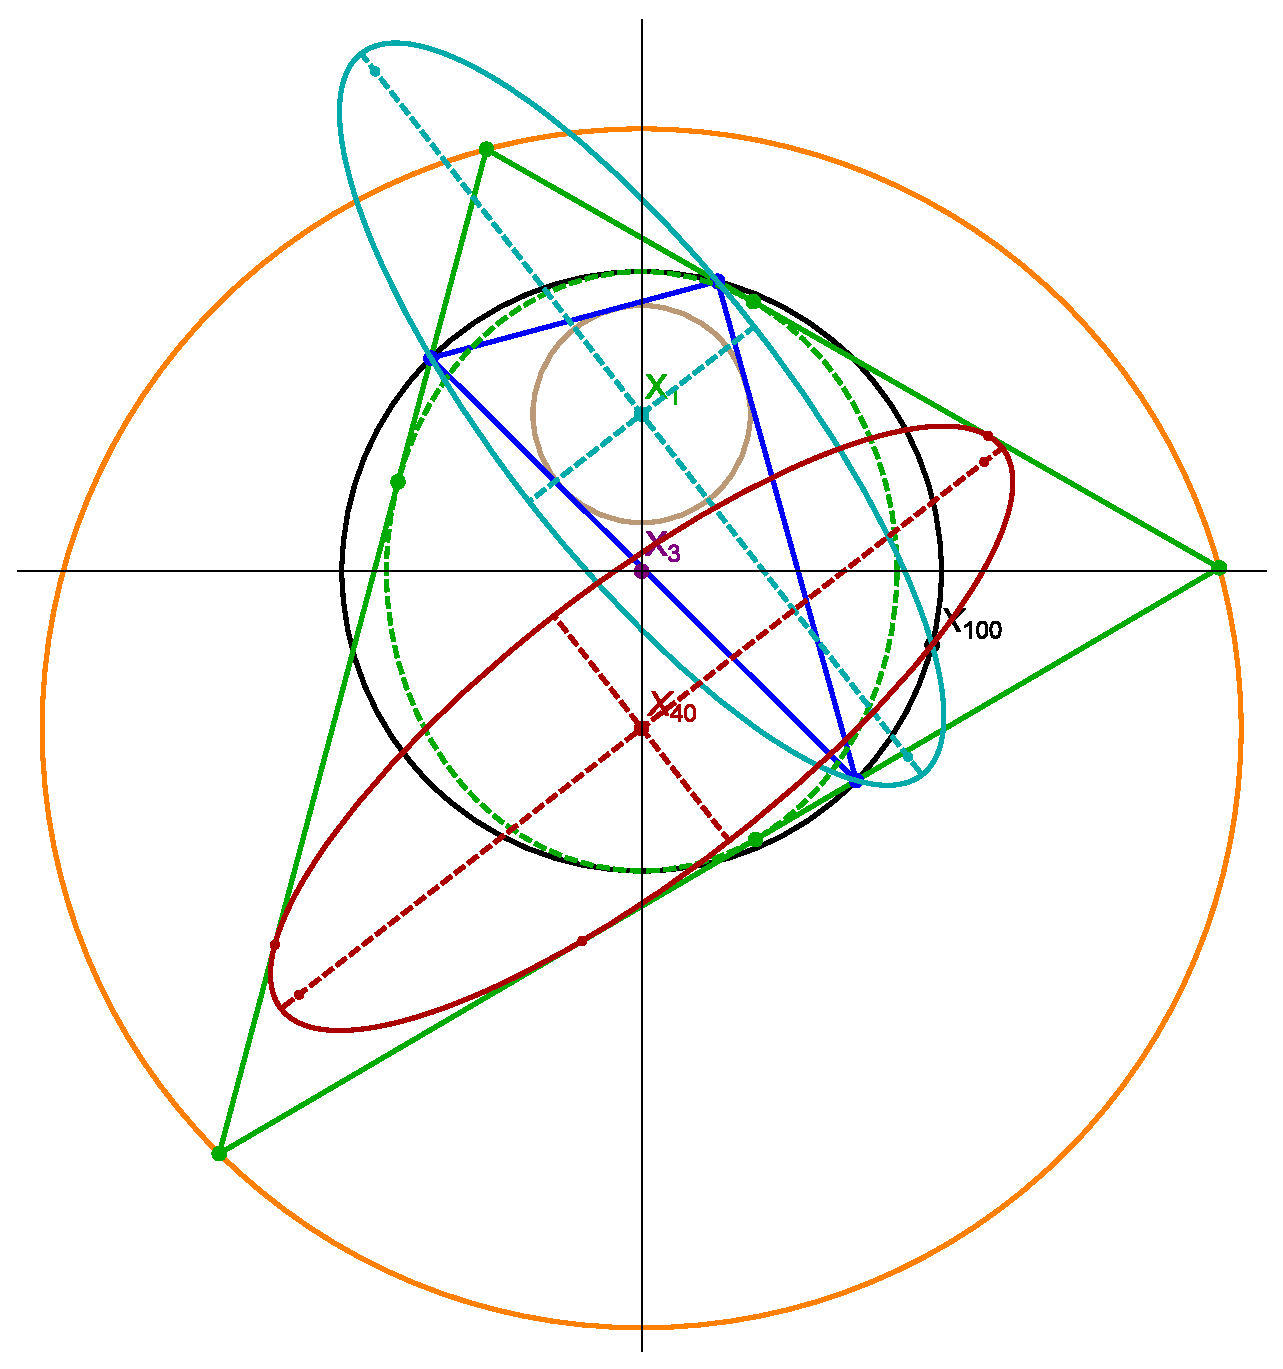
\includegraphics[width=.7\textwidth]{pics_03_230_excentral_poristic_inconics.eps}
    \caption{A poristic triangle (blue) is shown, as well as $I_1$, the $X_1$-centered inconic (light blue). Also shown is the excentral triangle (green), the circle (orange) the excentral family is inscribed in and their MacBeath caustic (dashed green). Also shown is $I_3'$ (dark red), the $X_3'$-centered excentral inconic (red). Note $X_3'=X_{40}$. Over the poristic family, both $I_1$ and $I_3'$ rotated rigidly at 90-degrees from each other. \href{https://youtu.be/hz0qEyVVvaI}{Video}}
    \label{fig:03-excentral-poristic-inconics}
\end{figure}

Given a triangle, an inconic is is fully defined by its center and is tangent to the three sidelines, see \cite[Inconic]{mw}.

Referring to \cref{fig:03-excentral-poristic-inconics}, let $E_1$ be the $X_1$-centered circumconcic to the poristic family, i.e., it contains the vertices. Let $\mu_1$, and $\nu_1$ denote its semi-axes. Interestingly:

\begin{proposition}
$\mu_1=R+d$ and $\nu_1=R-d$ are invariant over the poristic family, i.e., $E_1$ rigidly rotates about $X_1$. \label{prop:03-e1}
\end{proposition}

A proof appears in \cite[Appendix C]{garcia2020-similarity-I}.
\section{Poristic Excentrals}

\begin{figure}
    \centering
    %\includegraphics[width=.7\textwidth]{pics/0170_poristic.eps}
    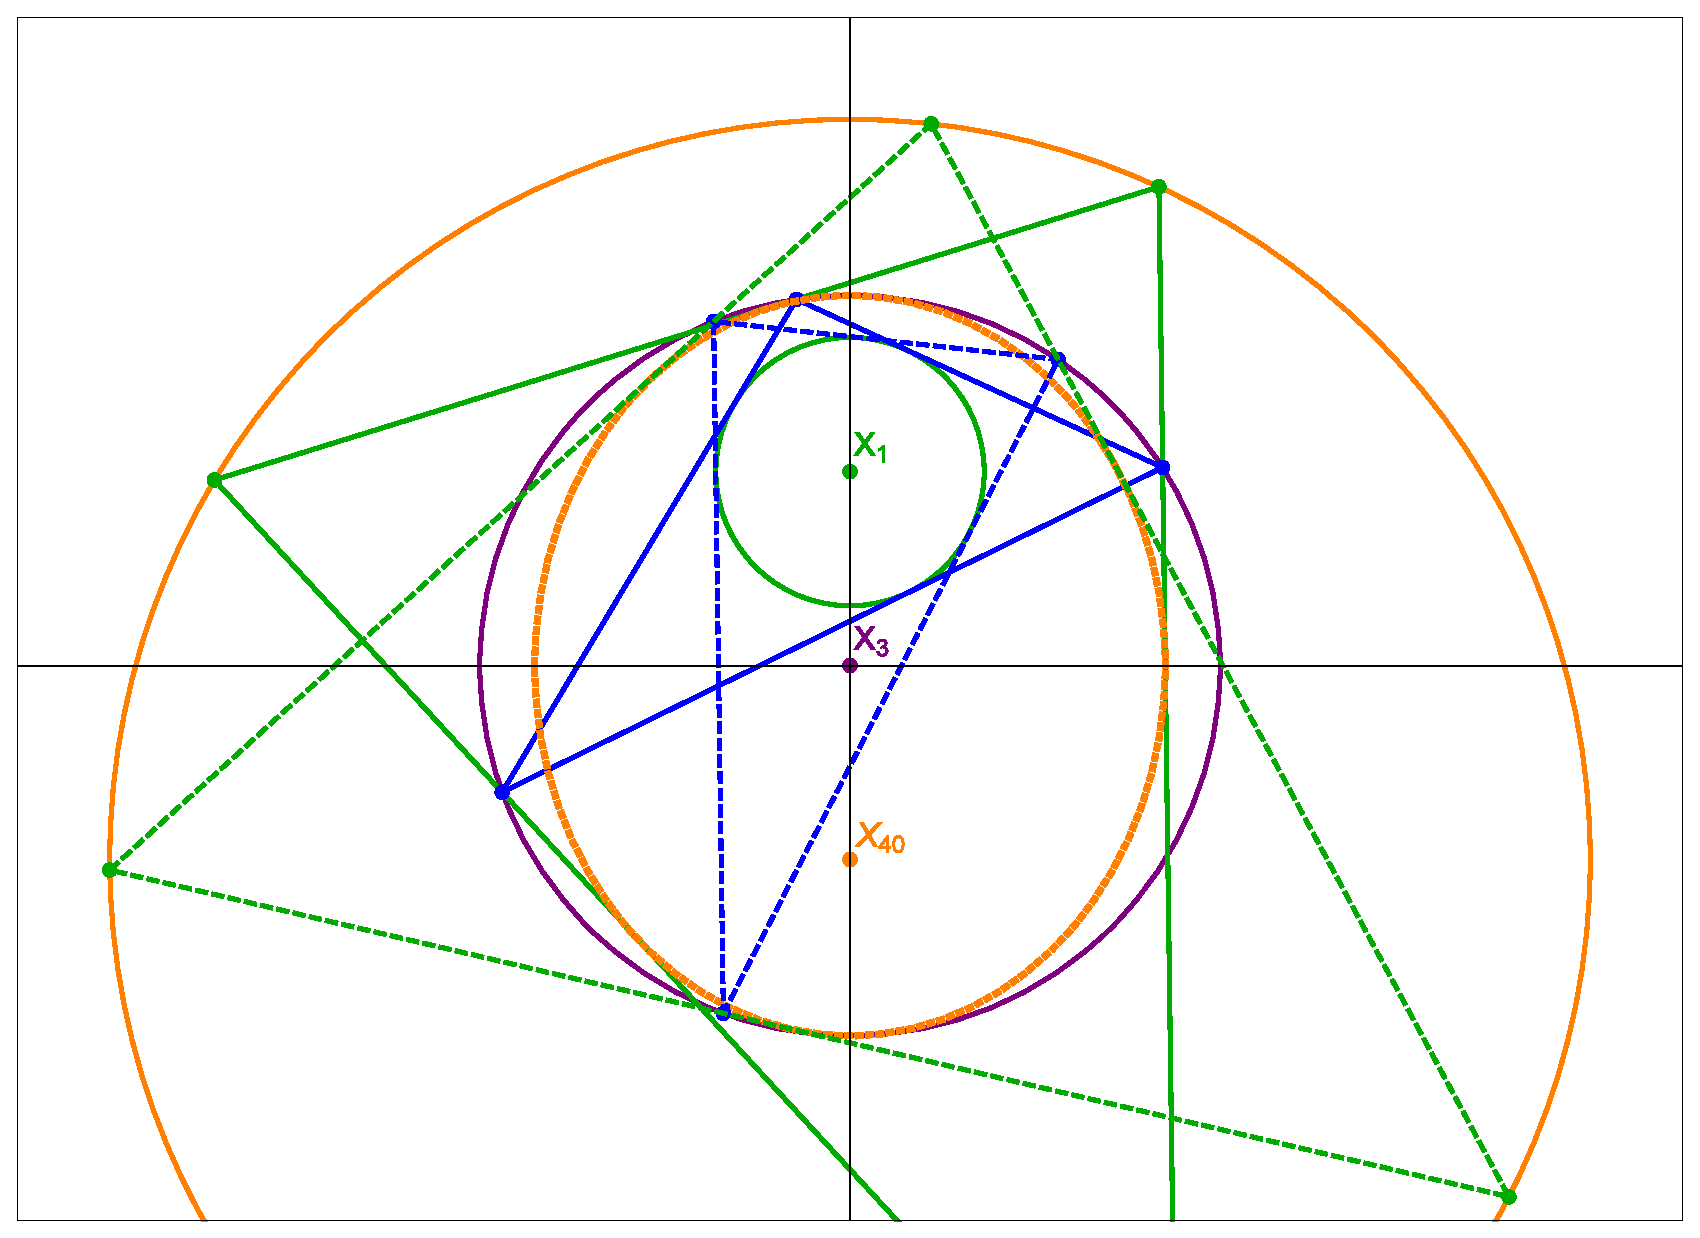
\includegraphics[width=\textwidth]{pics_03_170_poristic.eps}
    \caption{The poristic family (blue) is interscribed between two fixed circles, i.e., their circumcenter $X_3$ and incenter $X_1$ are stationary. The family of its excentral triangles (solid green) are inscribed in a circle (orange) centered on the Bevan point $X_{40}$ and of radius twice the original circumradius. This family circumscribes the MacBeath inellipse (dashed orange), centered on $X_3$ with foci on $X_1$ and $X_{40}$. A second for both poristics and excentrals configuration is also shown (dashed blue and dashed green).  \href{https://youtu.be/DS4ryndDK6Q}{Video}, \href{https://bit.ly/2RoYJHm}{Live}}
    \label{fig:03-poristic-excentrals}
\end{figure}

The family of excentral triangles to the poristic family, shown in \cref{fig:03-poristic-excentrals} is also Ponceletian: in \cite{odehnal2011-poristic}, it is shown to be inscribed in a circle of radius $2R$ where $R$ is the circumradius of its reference poristic family, centered on $X_{40}$, the Bevan point, or $X_3'$ of the family in questions (to avoid confusion, we will be priming quantities associated with this family).

\begin{proposition}
The barycenter $X_2'$ of poristic excentrals is stationary.
\end{proposition}

\begin{proof}
Recall a triangle's barycenter $X_2$ is a third of the way from the circumcenter to the orthocenter \cite[Euler Line, Eqn. 6]{mw}. The result follows from the fact that both $X_3'=X_{40}$ and $X_4'=X_1$ are stationary.
\end{proof}

The MacBeath inconic, defined in \cite[MacBeath Inconic]{mw}, is an ellipse centered on a triangle's 9-point center $X_5$, with  foci at the circumcenter $X_3$ and orthocenter $X_5$.

Poristic excentrals are Ponceletian since:

\begin{proposition}
The MacBeath inconic to the excentral poristics is stationary and is therefore the caustic. Let $\mu_5'$ and $\nu_5'$ denote its major and minor semi-axes. These are given by:
\[ \mu_5'=R,\;\;\;\nu_5'=\sqrt{R^2-d^2} \]
\end{proposition}

\begin{proof}
It is straightforward to verify the sidelines of poristic excentrals are dynamically  tangent to the ellipse:
\[
\frac{(x-d)^2}{R^2}+\frac{y^2}{R^2-d^2}=1\]
with center $X_3=(d,0)$ and foci $X_{40}=(0,0)$ and $X_1=(2d,0)$.
\end{proof}

Correspondences between the centers and foci of the excentral MacBeath inconic and those of the reference triangle appear in \cref{tab:03-macbeath}.

\begin{table}
\centering
\begin{tabular}{|c|c|c|}
\hline
\makecell[cc]{excentral\\ MacBeath} &
\makecell[cc]{excentral\\center} &
\makecell[cc]{reference\\center} \\
\hline
center & $X_5'$ & $X_3$\\
focus & $X_4'$ & $X_1$  \\
focus & $X_3'$ & $X_{40}$ \\
\hline
\end{tabular}
\caption{Center and foci of the MacBeath inconic of an excentral triangle and the corresponding triangle center of the reference.} 
\label{tab:03-macbeath}
\end{table}

Since $\mu'_5/\nu_5'=R/\sqrt{R^2-d^2}$, use \cref{eq:03-euler-poristic} to obtain:

\begin{corollary}
The aspect ratio of the caustic to the excentral poristics is given by:
\begin{equation*}
 \frac{\mu'_5}{\nu_5'}={\sqrt\frac{R}{2 r}}
\end{equation*}
\end{corollary}

As shown in \cref{fig:03-excentral-poristic-inconics}, let $I_3'$ be the $X_3'$-centered inconic to poristic excentrals. Let $\mu_3'$ and $\nu_3'$ denot its major and minor semi-axes, respectively.

\begin{proposition}
Over poristic excentrals,  $\mu_3'=R+d$ and $\nu_3'=R-d$ are invariant, i.e., $I_3'$ rigidly rotates about $X_3'$.
\label{prop:03-inconic-x3p}
\end{proposition}

We omit the long proof kindly contributed by B. Odehnal and appearing in \cite[Appendix C]{garcia2020-similarity-I}.

Interestingly:

\begin{theorem}
Excentral poristics are the image of the circumcircle family under a variable rigid rotation. The ridigly-rotating $I_3'$ is identified with the caustic of the circumcircle family.
\end{theorem} 

\begin{proof}
Recall \cref{prop:03-circumcircle-rh}: the orthic triangles of the circumcircle family has invariant inradius and circumradius. Also recall \cref{lem:03-circum-x5-locus}: the locus of the orthic circumcenter is a circle concentric with the common center. Also notice in the circumcircle family, the caustic is the stationary inconic centered on $X_3$.
\end{proof}

\section{The Brocard Porism}
 
A property-rich family of Poncelet triangles is the so-called ``Brocard porism'', introduced in  \cite{bradley2007-brocard,shail1996-brocard, bradley2011-brocard}. It is inscribed in a circle and circumscribes the so-called {\em Brocard inellipse}. Remarkably, its foci coincide with the stationary Brocard points $\Omega_1$ and $\Omega_2$ of the family; see \cref{fig:03-brocard-porism}.

Let $R$ denote the radius of the outer circle and $a',b'$ the caustic semi-axes, with $(c')^2=(a')^2-(b')^2$. Let also, $d=|X_{3}-X_{39}|$ the distance between the centers of the circle and of the caustic.

\begin{proposition}
A pair of circle (outer) $(x-x_0)^2+y^2=R^2$ and ellipse (caustic) $(x-x_1)^2/(a')^2+y^2/(b')^2=1$ admit a 1d family of Poncelet triangles if and only if 
\[(a')^2  - 2 R a'- (b')^2 +  R^2-d^2=0,\;\; d=|x_1-x_0| \]
\end{proposition}
\begin{proof}
  Follows from Cayley condition for 3-periodics in an NCAP pair.
  %\textcolor{red}{citar prop. cap 2}
\end{proof}
\begin{proposition}
For any triangle $T$, the circumcircle and Brocard inellipse are Ponceletian, they admit a 1d family of Poncelet triangles. Furthermore, their Brocard inellipse is stationary.
\label{prop:04-broc-inellipse-stationary}
\end{proposition}

\begin{proof}
Follows from vertex parametrization for the Brocard family and/or from stationarity of $X_6$, see \cref{prop:04-x6-stationary}. 
\end{proof}

\begin{proposition}
The stationary circumcenter $X_3$ and circumradius $R$ are given by:

\begin{equation}
X_3=[0,-\frac{c'\delta_1}{b'}],\;\;\;R= \frac{2 (a')^2}{b'} \\
 %=& \frac{\sqrt{3a^2+2c^2-2c\delta_1} (c +\delta_1)\delta_1}{ 3a^2b} 
 \label{eqn:broc-circumcircle}
\end{equation}
where $\delta_1=\sqrt{4 (a')^2-(b')^2}$.
\label{prop:cotw}
\end{proposition}

The following is a known requirement for the Brocard porism to be possible, appearing in \cite[Eqs. 15--17]{shail1996-brocard}:

\begin{corollary}
$R{\geq}2 c'$
\label{rem:minR}
\end{corollary}

Remarkably, and echoing a property seen above for the homothetic family, leaving the proof as an exercise:

\begin{proposition}
Over the Brocard porism, the Brocard angle $\omega$ is invariant and given by:
\[\cot\omega=\frac{\delta_1}{b'} \geq \sqrt{3} \]
\label{prop:03-brocard-w}
\end{proposition}

Henceforth we shall use symbol $\Sha$  $\cot\omega$. Recall for any triangle $\Sha=\sum_{i=1}^3{\cot{\theta_i}}$, i.e.:

\begin{corollary}
The Brocard porism conserves the sum of its internal angle cotangents.
\end{corollary}

\cite{shail1996-brocard} derives the distance between Brocard points (the foci of the Brocard inellipse), in terms of invariant $R$ and $\omega$:

\begin{equation} |{\Omega_1}-{\Omega_2}|^2=4 R^2\sin^2{\omega}(1-4\sin^2{\omega})=(c')^2
\label{eq:03-omega-dist}
\end{equation}

\begin{corollary}
\[ c' = R\sin{\omega}\sqrt{1-4\sin^2{\omega}} \]
\end{corollary}
 
 \begin{figure}
     \centering
     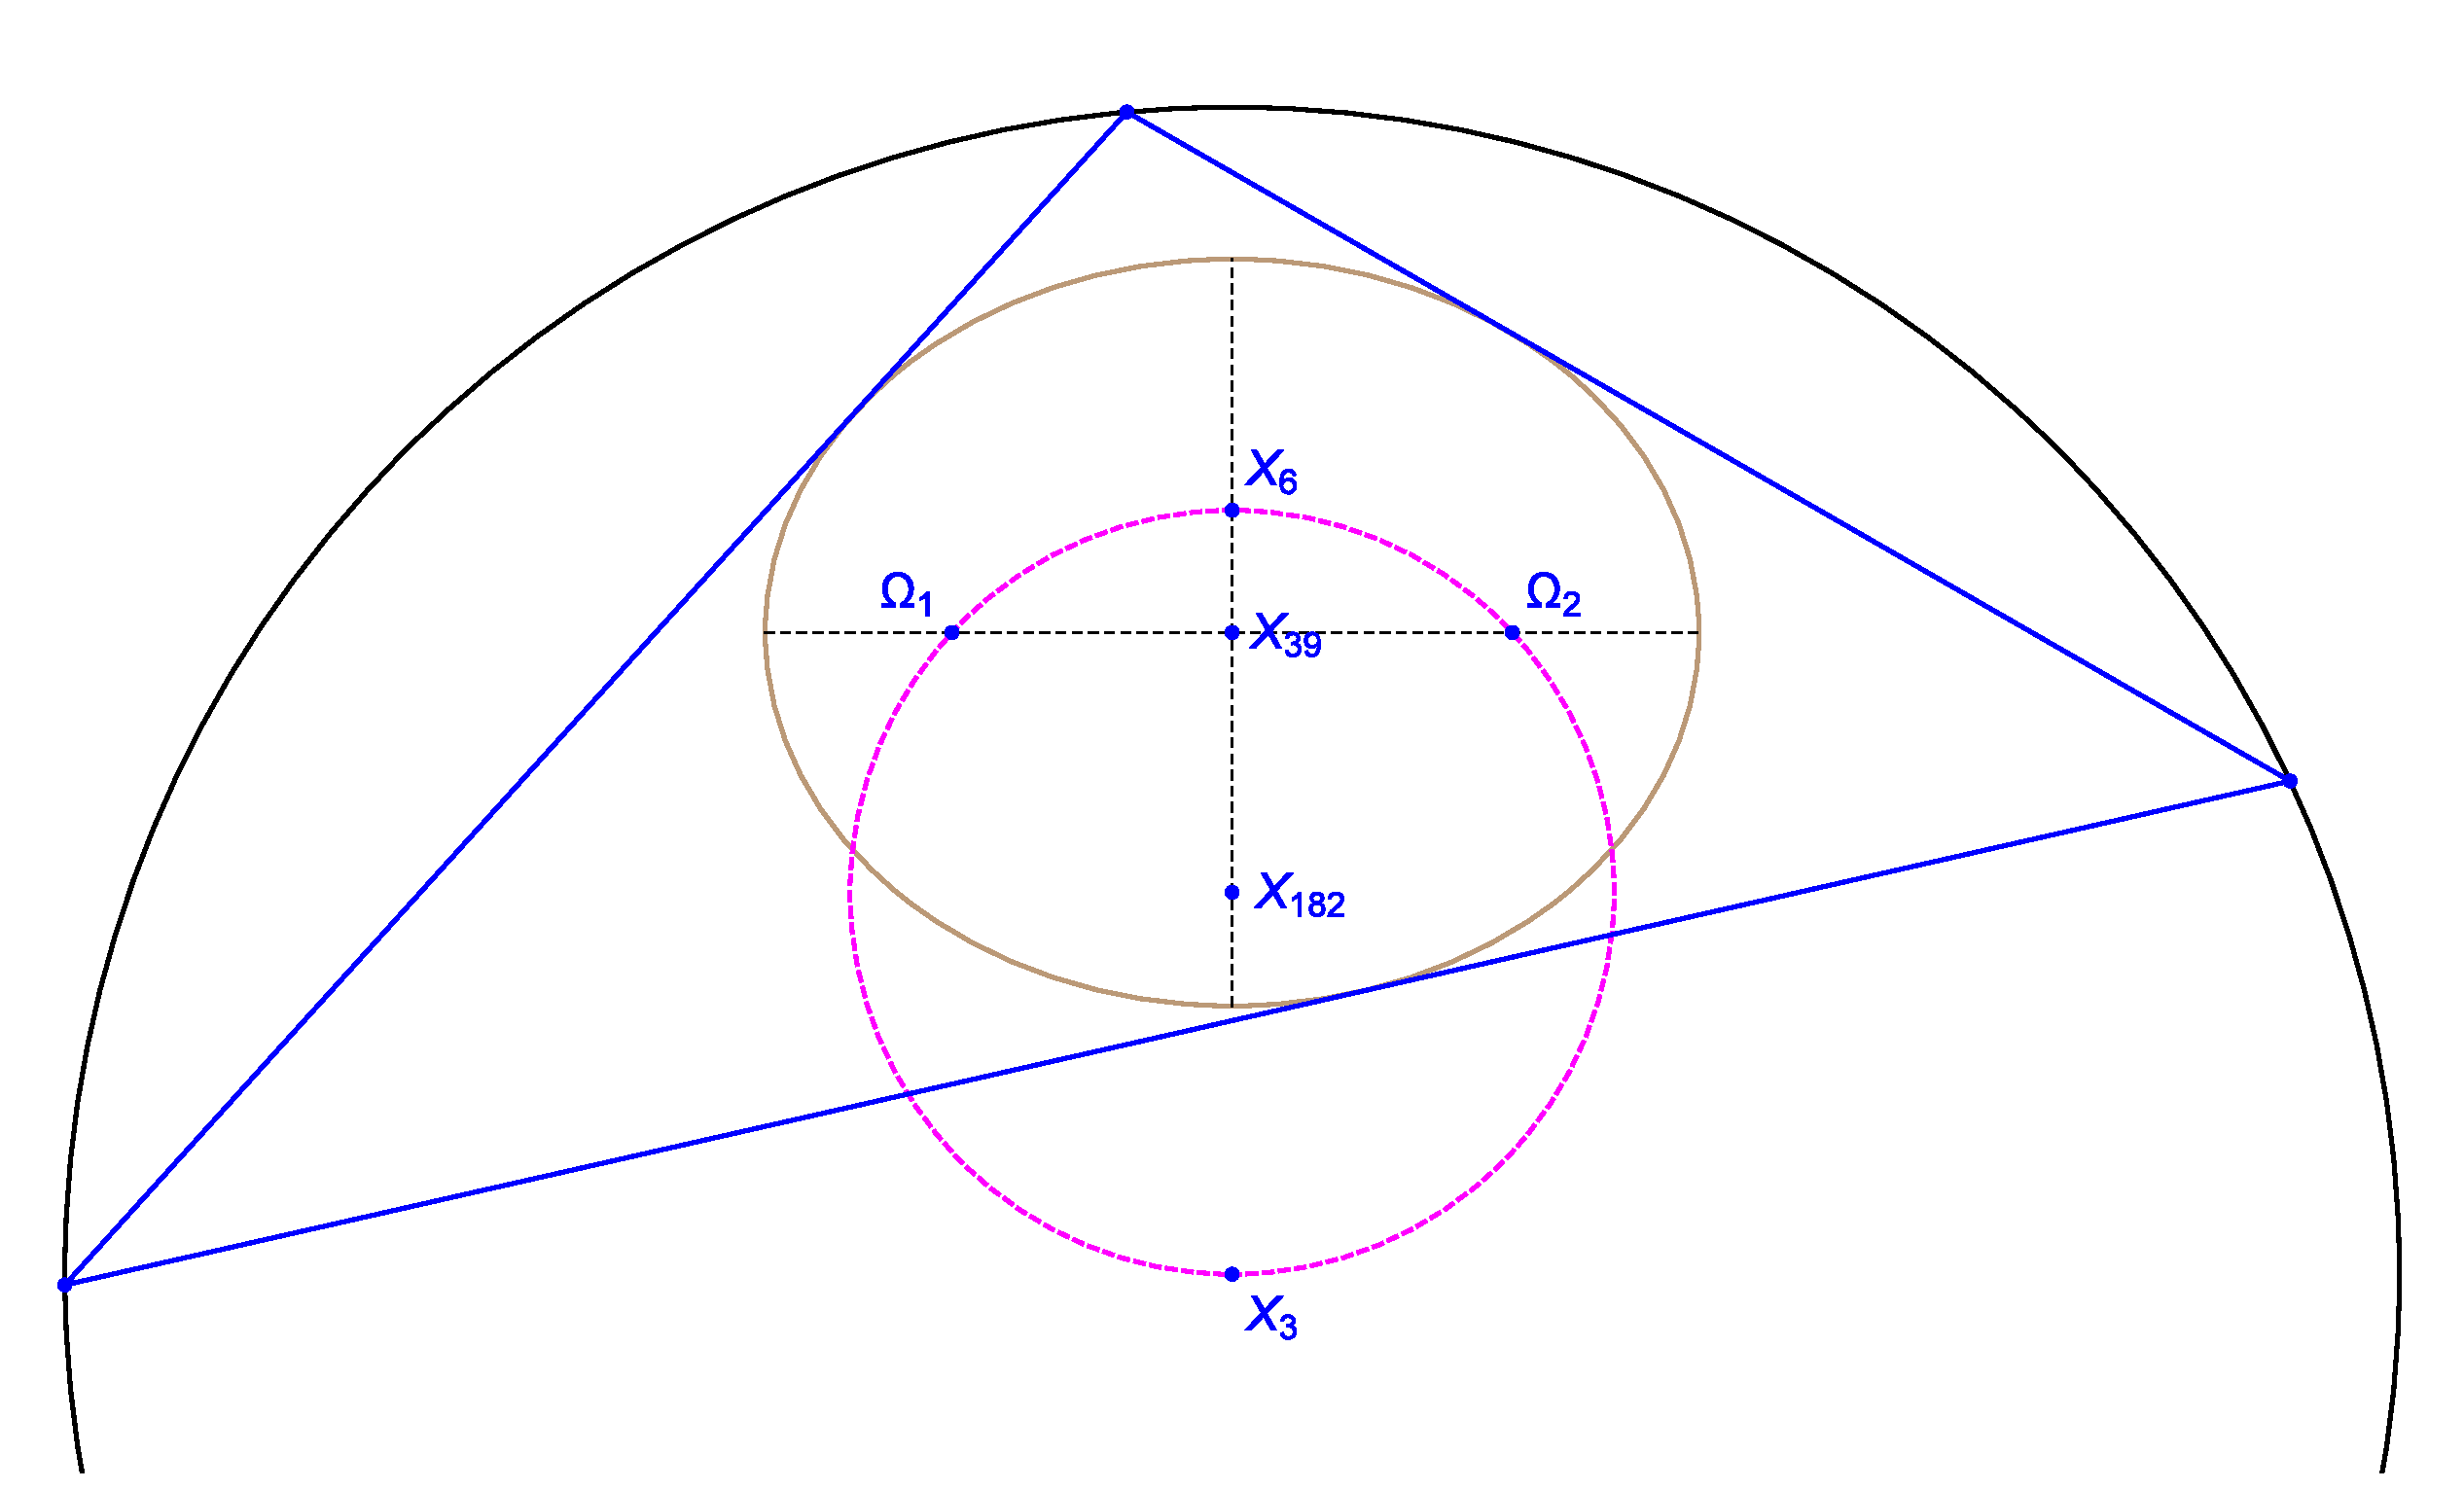
\includegraphics[width=\textwidth]{pics_03_240_brocard_porism.eps}
     \caption{A triangle (blue) in the Brocard porism is shown inscribed in an outer circle (black) and having the Brocard inellipse (brown) as its caustic, with foci at the stationary Brocard points $\Omega_1$ and $\Omega_2$ of the family, and centered on the Brocard midpoint $X_{39}$. The Brocard points as well as the stationary circumcenter $X_3$ and symmedian point $X_6$ are concyclic on the Brocard circle (dashed magenta), whose center is $X_{182}$. \href{https://bit.ly/2QX3lEt}{Live}}
     \label{fig:03-brocard-porism}
 \end{figure}

Referring to \cref{fig:03-brocard-porism}, all of $\Omega_1$, $\Omega_2$, $X_3$, and $X_6$ are concyclic on the so-called Brocard circle, see \cite[Brocard Circle]{mw}, whose center is $X_{182}$. The Brocard axis is defined in \cite[Brocard Axis]{mw} as the line containing the circumcenter $X_3$ and symmedian point $X_6$ of a triangle.
 
\begin{proposition}
Over the Brocard porism, the following 3 objects are stationary: (i) the Brocard circle, (ii) the Brocard axis, and (iii) the symmedian point $X_6$ are stationary.
\label{prop:04-x6-stationary}
\end{proposition}

\begin{proof}
The Brocard circle is stationary since it passes through 3 stationary points: $\Omega_1,\Omega_2,X_3$ are stationary. The Brocard axis is stationary since it contains stationary $X_3$ and stationary Brocard midpoint $X_{39}$. For any triangle, $X_6$ is antipodal to $X_3$ on the Brocard circle.
\end{proof}
 
Recall the two isodynamic points $X_{15}$ and $X_{16}$ of a triangle as the two unique intersections of the 3 Apollonius circles\footnote{These are circles which contain a vertex and the intersection of the corresponding internal and external bisectors with the opposite side.}. $X_{15}$ (resp. $X_{16}$) is interior (resp. exterior) to the circumcircle. In fact they are inverse images of each other with respect to the latter, see \cite[Isodynamic Points]{mw}.

\begin{proposition}
Over the Brocard porism, the two Isodynamic points $X_{15}$ and $X_{16}$ are stationary and given by:

\[
X_{15}=\left[0, \frac{R(\sqrt{3}-\Sha)}{
 \sqrt{\Sha^2-3}}\right],\;\;\;
 X_{16}=\left[0, -\frac{R(\sqrt{3}+\Sha)}{
 \sqrt{\Sha^2-3}}\right]
\]
\label{prop:03-x15x16}
\end{proposition}

\begin{proof}
Let $P$ and $U$ be finite points on a triangle's plane with normalized barycentric coordinates $(p,q,r)$ and $(u,v,w)$, respectively. Let $f$ and $g$ be homogeneous functions of the sidelengths. The $(f,g)$ {\em barycentric combo} of $P$ and $U$, also denoted $f*P + g*U$, is the point with barycentrics $(f\,p + g\,u,f\,q + g\,v, f\,r + g\,w)$. In \cite[X(15), X(16)]{etc}, the following combos (see below), derived by Peter Moses, are provided:

\begin{align}
X_{15} =& \sqrt{3}*X_3 + \Sha*X_6 \label{eqn:combo-x15} \\
X_{16} =& \sqrt{3}*X_3 - \Sha*X_6 \nonumber
\end{align}
 
 With all involved quantities invariant, the result follows.
\end{proof}

\begin{proposition}
The semi-axes $a'$ and $b'$ and center $X_{39}$ of the Brocard inellipse are given by:

\begin{gather*}
[a',b']= R\left[\sin\omega,2\sin^2\omega\right]=R\left[\frac{1}{\sqrt{1+\Sha^2}},\frac{2}{{1+\Sha^2}}\right]\\
 X_{39}=\left[0,-\frac{R\Sha\sqrt{\Sha^2-3}}{\Sha^2+1}\right]
\end{gather*}
 \label{prop:03-brocard-axes}
\end{proposition}

\begin{proof}

Consider a triangle $T$ with sidelengths $s_1,s_2,s_3$, area  $\Delta$, and circumradius  $R$. The following identities appear in \cite{bradley2007-brocard,shail1996-brocard}:

\begin{equation}
R=\frac{s_1 s_2 s_3}{4\Delta}, \;\;\; \sin\omega=\frac{2\Delta}{\sqrt{\Gamma}}
\label{eq:03-broc-R-sinw}
\end{equation}

\noindent where $\Gamma=(s_1 s_2)^2+(s_2 s_3)^2+ (s_3 s_1)^2$. Bringing in \cref{eq:03-omega-dist}, the result follows from combining the above into expressions for the Brocard inellipse semi-axes given in \cite[Brocard Inellipse]{mw}:

\begin{equation}
a' =\frac{s_1 s_2 s_3}{2\sqrt{\Gamma}},\;\;\;\;\;\;b' =\frac{2 s_1 s_2 s_3 \Delta}{\Gamma}
\label{eq:03-broc-axes}
\end{equation}

\end{proof}

With the results above, we can derive the following quantities and centers explicitly:

\begin{align*}
X_6&=\left[0,-\frac{R\sqrt{ \Sha^2 -3}}{ \Sha}\right] \\
|X_3-X_6|&=\frac{R\sqrt{ \Sha^2 -3}}{ \Sha}\\
\Omega_{1,2}(R,\Sha)&=\frac{R\sqrt{ \Sha^2-3}}{ \Sha^2+1} \left[ \pm 1, - \Sha  \right]
%X_{39}&=\left[0,-R {\frac {\Sha\,\sqrt {\Sha^2-3}}{\Sha^2+1}} \right]
\end{align*}

Let $a'$ be the major axis of a generic triangle's Brocard inellipse. Interestingly, we have:

\begin{lemma}
\[ \sum_{i=1}^{3}{\frac{1}{s_i^2}}=\frac{1}{4 (a')^2} \]
\end{lemma}

\begin{proof}
As
\[\frac{1}{s_1^2}+\frac{1}{s_2^2}+\frac{1}{s_3^2}=\frac{s_2^ 2s_3^2+s_1^2 s_3^2+s_1^2 s_2^2}{s_1^2 s_2^2 s_3^2}\]
the result follows from \cref{eq:03-broc-axes}.  
\end{proof}

\noindent Therefore, we have:

\begin{corollary}
Over the Brocard porism, the sum of inverse squared sidelengths is invariant
\end{corollary}

\noindent \textbf{Similarity and Polar image:} As it will be seen below, the Brocard porism is the image of the Homothetic family under two different transformations: variable similarity and polar.

Referring to \cref{fig:03-homot-broc-inell}, we will first prove a handy lemma, introduced in  \cite{reznik2020-similarityII}:

\begin{figure}
    \centering
    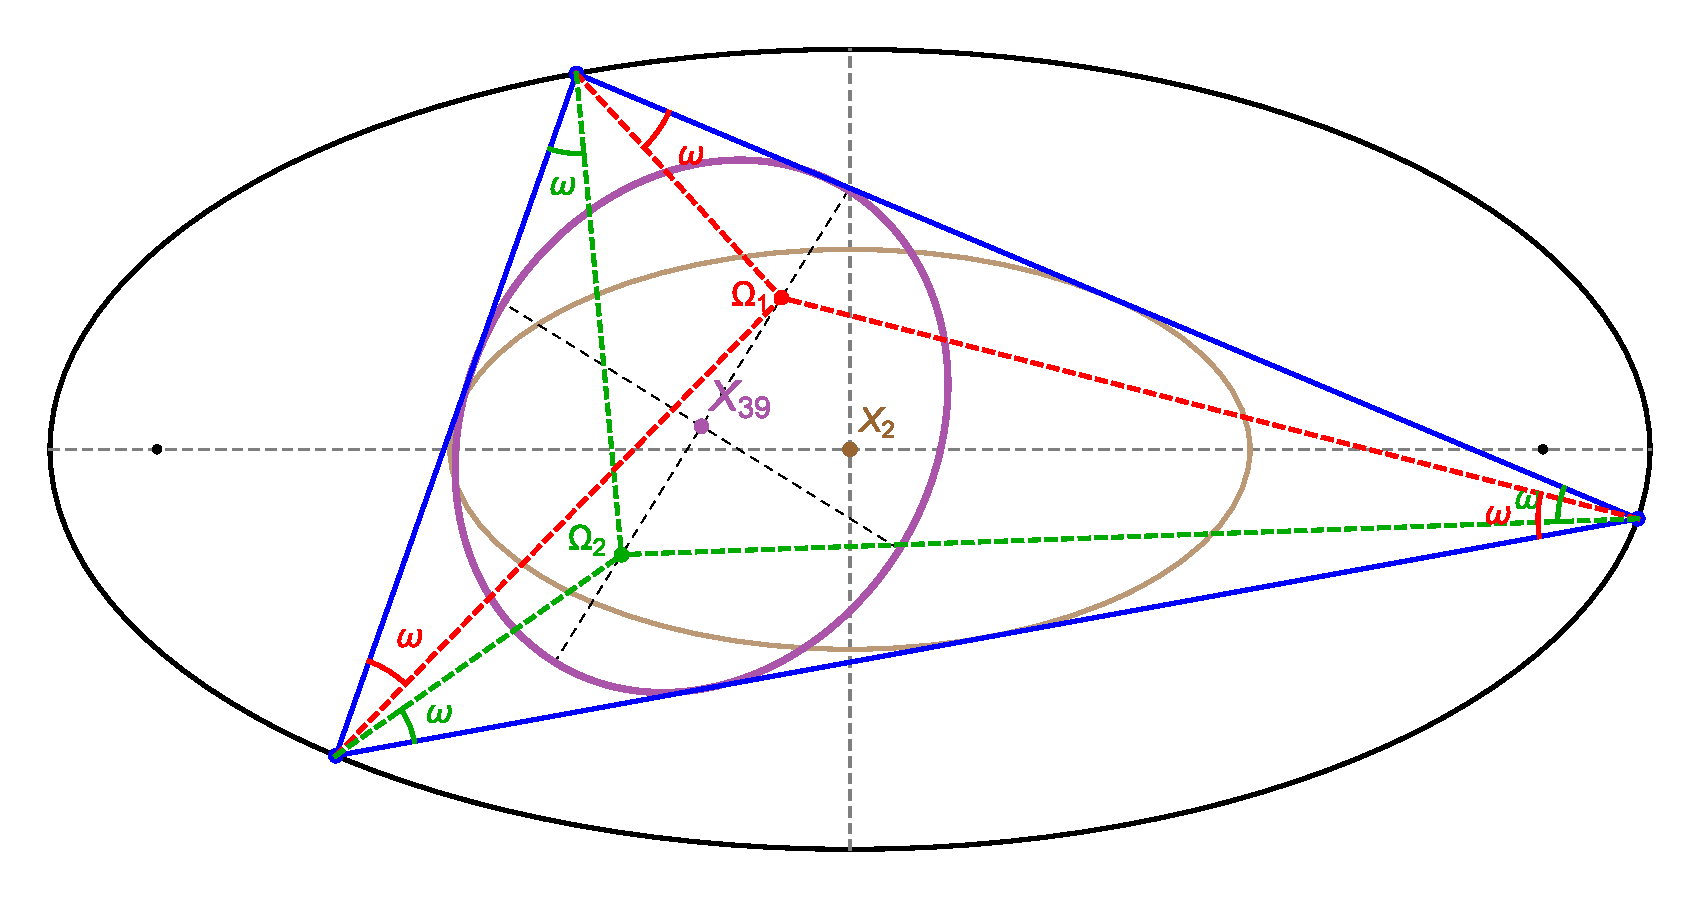
\includegraphics[width=\textwidth]{pics_03_270_homot_broc_inell.eps}
    \caption{Over the homothetic family, the Brocard inellipse has semi-axes of variable lengths but invariant aspect ratio. \href{https://youtu.be/DIm2qTxGWXE}{Video}}
    \label{fig:03-homot-broc-inell}
\end{figure}

\begin{lemma}
Over the homothetic family, though the semi-axes of the Brocard inellipse have variable lengths, their ratio $\beta$ is invariant and given by:
\[\beta=
\frac{\sqrt{3a^4+10a^2b^2+3b^4}}{4ab} > 1\]
\label{lem:03-beta}
\end{lemma}

\begin{proof}
The result follows from combining \cref{eq:03-broc-R-sinw} with \cref{eq:03-broc-axes}, using the sidelengths $s_i$ of the homothetic family using the parametrization in \cref{sec:03-vtx-param}.
\end{proof}

The result below was introduced in \cite[Thm 4.1]{reznik2020-similarityII}:

\begin{proposition}
The Brocard family is the image of the homothetic one under a variable similarity transform.
\end{proposition}

\begin{proof}
Consider the following similarity transform which sends points $X$ in the plane of the homothetic family to new ones $X'$:

\[X'=Scale(1/b'').Rot(-\theta).Transl(-X_{39}).X\]

\noindent where  $b''$ is the variable minor semi-axis length of the the (moving) Brocard inellipse $\E''$ in the homothetic pair, $\theta$ the angle between said minor axis and the horizontal, and $X_{39}$ the moving center of $\E''$. Clearly, $\E''$ will be sent to an origin-centered ellipse which is axis-parallel to the homothetic ones. By Lemma~\ref{lem:03-beta}, the aspect ratio $\beta$ of $\E''$ is invariant over the homothetic family, implying the transformed inellipse will have fixed axes $(\beta, 1)$. Notice its circumcenter and circumradius are prescribed by the semi-axes of the caustic (Equation~\ref{eqn:broc-circumcircle}). This completes the proof. 
\end{proof}

\begin{figure}
    \centering
    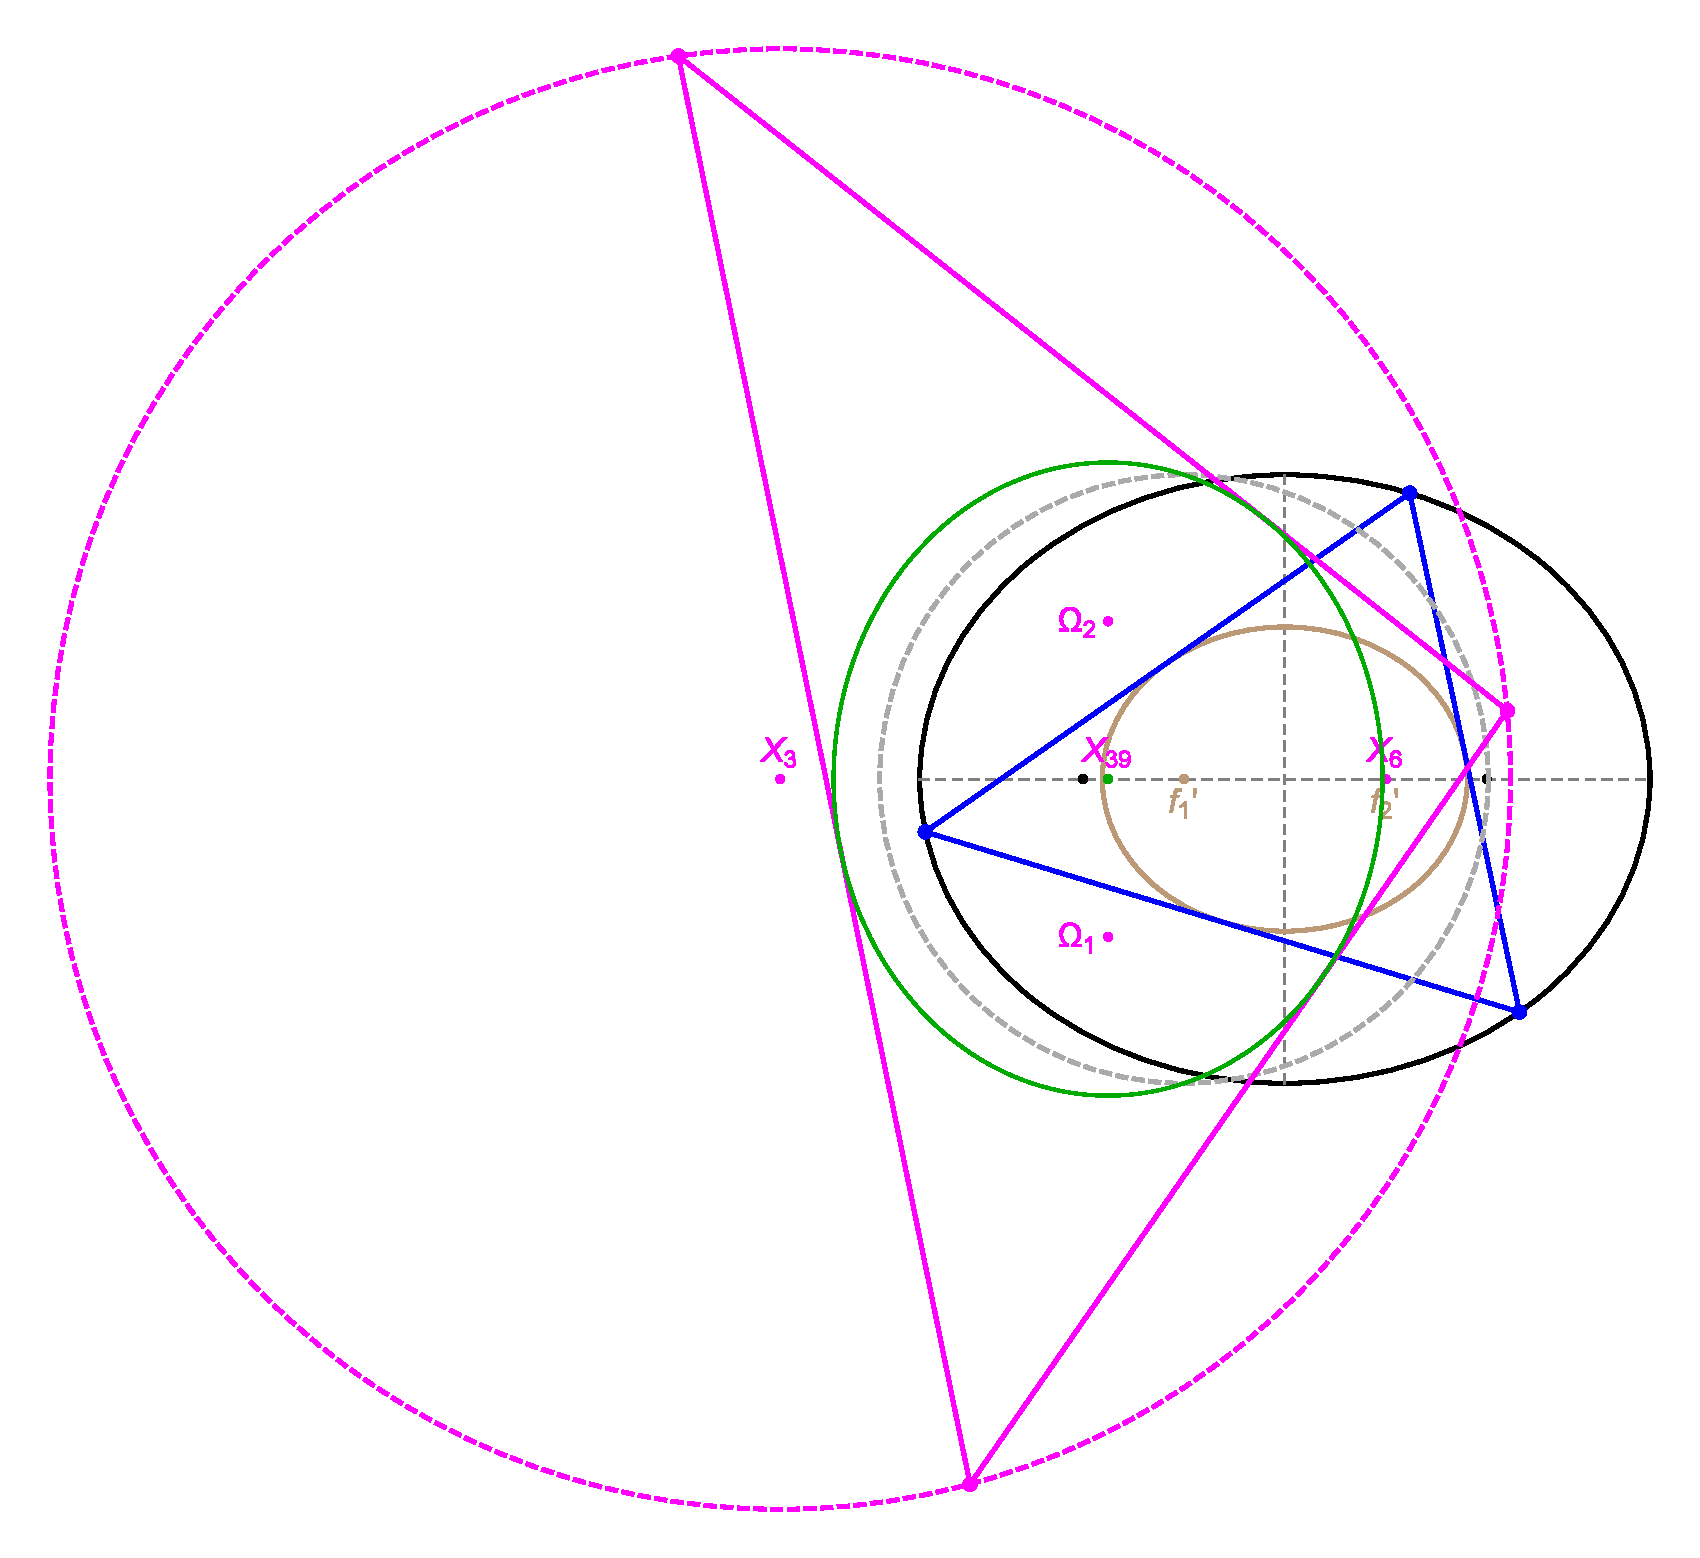
\includegraphics[width=.7\textwidth]{pics_03_260_brocard_homothetic_polar.eps}
    \caption{The Brocard family (magenta) is the polar image of the homothetic family (solid blue) with respect to a circle (dashed gray) centered on a focus of the homothetic caustic (light brown) which is sent to the Brocard circumcircle (dashed magenta). The outer ellipse (black) is sent to the Brocard inellipse (green). \href{https://bit.ly/2RwKmAM}{Live}}
    \label{fig:03-brocard-homoth}
\end{figure}

Referring to \cref{fig:03-brocard-homoth}, let $a,b$ be the semi-axes of the outer ellipse in the homothetic pair. 

\begin{proposition}
The Brocard porism is the polar image of the homothetic family with respect to a circle centered on a caustic focus $f'$.  The symmedian point $X_6$ of the image coincides with $f'$. Its outer circle and ellipse are given by:
\begin{align*}
   \mathcal{C}:&\;\; (x-x_0)^2+y^2  =R^2 \\
  \mathcal{E}:& \;\;  \frac{(x-x_1)^2}{(a')^2}+\frac{y^2}{(b')^2}=1\\
    x_0&=-\frac{c(b^2 + 4\rho^2)}{2b^2},\;\; 
    x_1 =  -\frac{c(4a^2 - c^2 + 4\rho^2)}{2(4a^2 - c^2)}\\
    (a')&= \frac{4a\rho^2}{4a^2 - c^2},\;\;
    (b') = \frac{2a\rho^2 }{b\sqrt{4a^2 - c^2}},\;\; R=\frac{2a\rho^2}{b^2} 
\end{align*}
Here $b'>a'$.
\label{prop:03-brocard-polarimage}
\end{proposition}
 
\begin{proof}
Proof is left as an exercise.
\end{proof}

%%% It follows from the same approach developed in \cref{sec:09-polarimage}.  Details are left to the reader.
\begin{remark}
 From the relations obtained in \cref{prop:03-brocard-polarimage} it follows that
 \[a=\rho^2\frac{(4 (b')^2-(a')^2)}{3 a' (b')^2},\;\; b=\rho^2\frac{\sqrt{4 (b')^2-(a')^2}}{\sqrt{3} (b')^2}\]
 
\end{remark}

Since two polar transformations with respect to the same circle is the identity:

\begin{corollary}
The homothetic family is the polar image of the Brocard family with respect to its stationary symmedian point $X_6$.
\end{corollary}
  
\begin{corollary}
In terms of the homothetic pre-image semi-axes $a,b$, the invariant sum of inverse squared sidelengths and Brocard angle are given by:
 
\begin{align*}
\sum_{i=1}^{3}{\frac{1}{s_i^2}}&=\frac{1}{4 (b')^2}=\frac{b^2(3a^2 + b^2)}{ 16\rho^4a^2}  \\
 \cot\omega&=\Sha=\sqrt{3}\frac{a }{b } 
\end{align*}
\end{corollary}

\begin{proof} By \cref{prop:03-brocard-axes} and \cref{prop:03-brocard-polarimage} it follows that
  $\sin\omega=(a')/(2b')=b/\sqrt{4a^2-c^2}.$
Using that $\csc^2\omega-\cot^2\omega=1$ the result follows.
\end{proof}

\section{Vertex Parametrization}

\subsection{Poristic family}
\label{sec:04-vtx-poristic}

Consider a pair of circles $x^2+y^2=R^2$,
$(x-d)^2+y^2=r^2$, with $d^2=R(R-2r)$. Then a 3-periodic orbit is parametrized by:

\begin{align}
P_1&=[x_1,y_1]\nonumber \\
 P_2&=\frac{1}{w^2} [ -4R r^2 q  y_1 - w_1w_2 , -2r R w_1y_1 + 2 r q w_2 ]\nonumber \\
  P_3 &=  \frac{1}{w^2} [4R r^2 q  y_1 - w_1w_2 , -2r R w_1y_1 - 2 r q w_2 ]\label{eq:04-vtx-poristic} \\
  q&=\sqrt{R^2 - r^2 - 2d x_1  + d^2},\;\; w=R^2 - 2d x_1  + d^2\nonumber 
  \\ w_1&=R^2 - 2r^2 - 2 d x_1 + d^2,\;\;\;
  w_2=(R^2+d^2) x_1 - 2 R^2 d  \nonumber
\end{align}

\subsection{Poristic Excentrals}

Its vertices sweep a circle centered on $X_{40}$ of the original poristic family, so we omit the parametrization.

\subsection{Brocard Porism}

Consider an isosceles Poncelet triangle $\Tm=ABC$ in the Brocard porism, where $AB$ is tangent to $\E$ at one of its minor vertices. Let $|AB|=2d$ and the height be $h$. Let $\zeta=d^2+h^2$. Let the origin $(0,0)$ be at its circumcenter $X_3$. Its vertices will be given by:

\[A=\left[-d ,\frac{d^2-h^2}{2h}\right], \;\;\; B= \left[d,\frac{d^2-h^2}{2h}\right], \;\;\; \left[0 ,\frac{\zeta}{2h}\right] \]


\begin{proposition}\label{prop:pair_brocard}
The Brocard porism containing $\Tm$ as a Poncelet triangle is defined by the following circumcircle $\K_0$ and Brocard inellipse $\E$:

\begin{align*}
\K_0:&\, x^2+y^2-R^2=0, \;\;\; R=\frac{\zeta}{2h}\\
\E:&\, -64d^2  h^4  x^2-4  h^2  (9  d^2+h^2)  \zeta  y^2 +4  h  (3  d^2+h^2)  (3  d^2-h^2)  \zeta  y\\&-(d^2-h^2) (9d^2 -h^2) \zeta^2=0
\end{align*}
\end{proposition}

\begin{proof}
The proof follows from $\Tm$, and isosceles Poncelet triangle. Recall that the Brocard inellipse is centered at $X_{39}$. Its perspector is $X_6$, i.e., it will be tangent to $\Tm$ where cevians through $X_6$ intersect it; see \cite[Brocard inellipse]{mw}.
\end{proof}

Consider the pair: circle $x^2+y^2=R^2=(d^2+h^2)^2/(4h^2)$ and   ellipse
$x^2/a^2+(y-y_0)^2/b^2=1$, with  semi-axes
 \[  (a,b)=\left(\frac{d\sqrt{d^2+h^2}}{9d^2+h^2},\frac{4d^2}{9d^2+h^2}\right)
    \]
and center $(0,y_0)$,  $y_0=(9d^4 - h^4)/(2h(9d^2  +  h^3))$.

Vertices $P_i=[x_i,y_i]$, $i=1,2,3$ of Brocard porism triangles are given by:

{\small  
\begin{equation}
    \aligned
    x_1 &= \cos{t}/q_1\\
    y_1 &= \sin{t}/q_1 \\
    x_2 &= -d (d^2 + h^2) ((3 d^2 + h^2)\sin{t} + 2d h \cos{t}- 3 d^2 + h^2)/q_2 \\
    y_2&=-(d^2 + h^2) ((9 d^4 - 2 d^2 h^2 + h^4)\sin{t} - 2 d h (3 d^2 + h^2)\cos{t} - 9 d^4 + h^4)/(2 b q_2) \\
    x_3 &= d (d^2 + h^2) (2 d h \cos{t} - (3 d^2 + h^2) \sin{t} + 3 d^2 - h^2)/q_3\\
    y_3 &=(d^2 + h^2) (2d h (3 d^2 + h^2) \cos{t}+ (9 d^4 - 2 d^2 h^2 + h^4)\sin{t} - 9 d^4 + h^4)/(2 b q_3) \\
    q_1&=(2h)/(d^2+h^2)\\
    q_2&= 2 d h (3 d^2 - h^2)\cos{t} - (9 d^4 - h^4) \sin{t}  + 9 d^4 + 2 d^2 h^2 + h^4\\
    q_3&= 2 d h (3 d^2 - h^2)\cos{t} + (9 d^4 - h^4)\sin{t} - 9 d^4 - 2 d^2 h^2 - h^4
\endaligned
\label{eqn:03-vertices-brocard}
\end{equation}
}

\section{Summary}

Fixed points and (known) conserved quantites for the non-concentric (NCAP) families in chapter appear in
\cref{tab:n3-non-conc-families} (compare with 
\cref{tab:n3-conc-families}).

A diagram depicting how certain pairs of families are interrelated by either similarity or polar transformations appears in in \cref{fig:03-transformations}.

\begin{table}
\centering
\begin{tabular}{|r|c|c|l|}
\hline
Family & Fixed & Conserves & Notes \\
\hline
\makecell[rc]{Poristic\\(bicentric)} & $X_1$, $X_3$, $X_{40}$, $\ldots$ & $\sum\cos\theta_i,a_9/b_9$ & \makecell[lc]{polar image of Confocal family\\wrt to a focus} \\
\hline
\makecell[rt]{Poristic\\Excentrals} & $X_2$, $X_3$, $X_4$, $X_5$ & $\sum{s_i^2}$, $\prod\cos\theta_i$ & \makecell[lt]{Inscribed in circle;\\caustic is MacBeath inconic} \\
\hline
Brocard & \makecell[lc]{$X_3$, $X_6$, $X_{15}$, $X_{16}$,\\$X_{39}$, $X_{182},\ldots$,\\$\Omega_1$, $\Omega_2$} & $\sum{s_i^{-2}}$, $\omega$, $\sum\cot\theta_i$ & \makecell[lc]{polar image of Homothetic\\family wrt caustic focus;\\inscribed in circle;\\caustic is Brocard inellipse}\\
%\hline
%focus-Inversive & $X_7$ & $L,\sum\cos\theta_i$ & \makecell[lc]{inversive image of Confocals\\wrt a focus; non-Ponceletian;\\inscribed in Pascal's limaçon;\\caustic non-ellipse}\\
\hline
\end{tabular}
\caption{Summary of fixed points and (known) conserved quantites for the non-concentric, axis-parallel (NCAP) families in this chapter.}
\label{tab:n3-non-conc-families}
\end{table}

% \includegraphics[trim={left bot right top},clip]
\begin{figure}
    \centering
    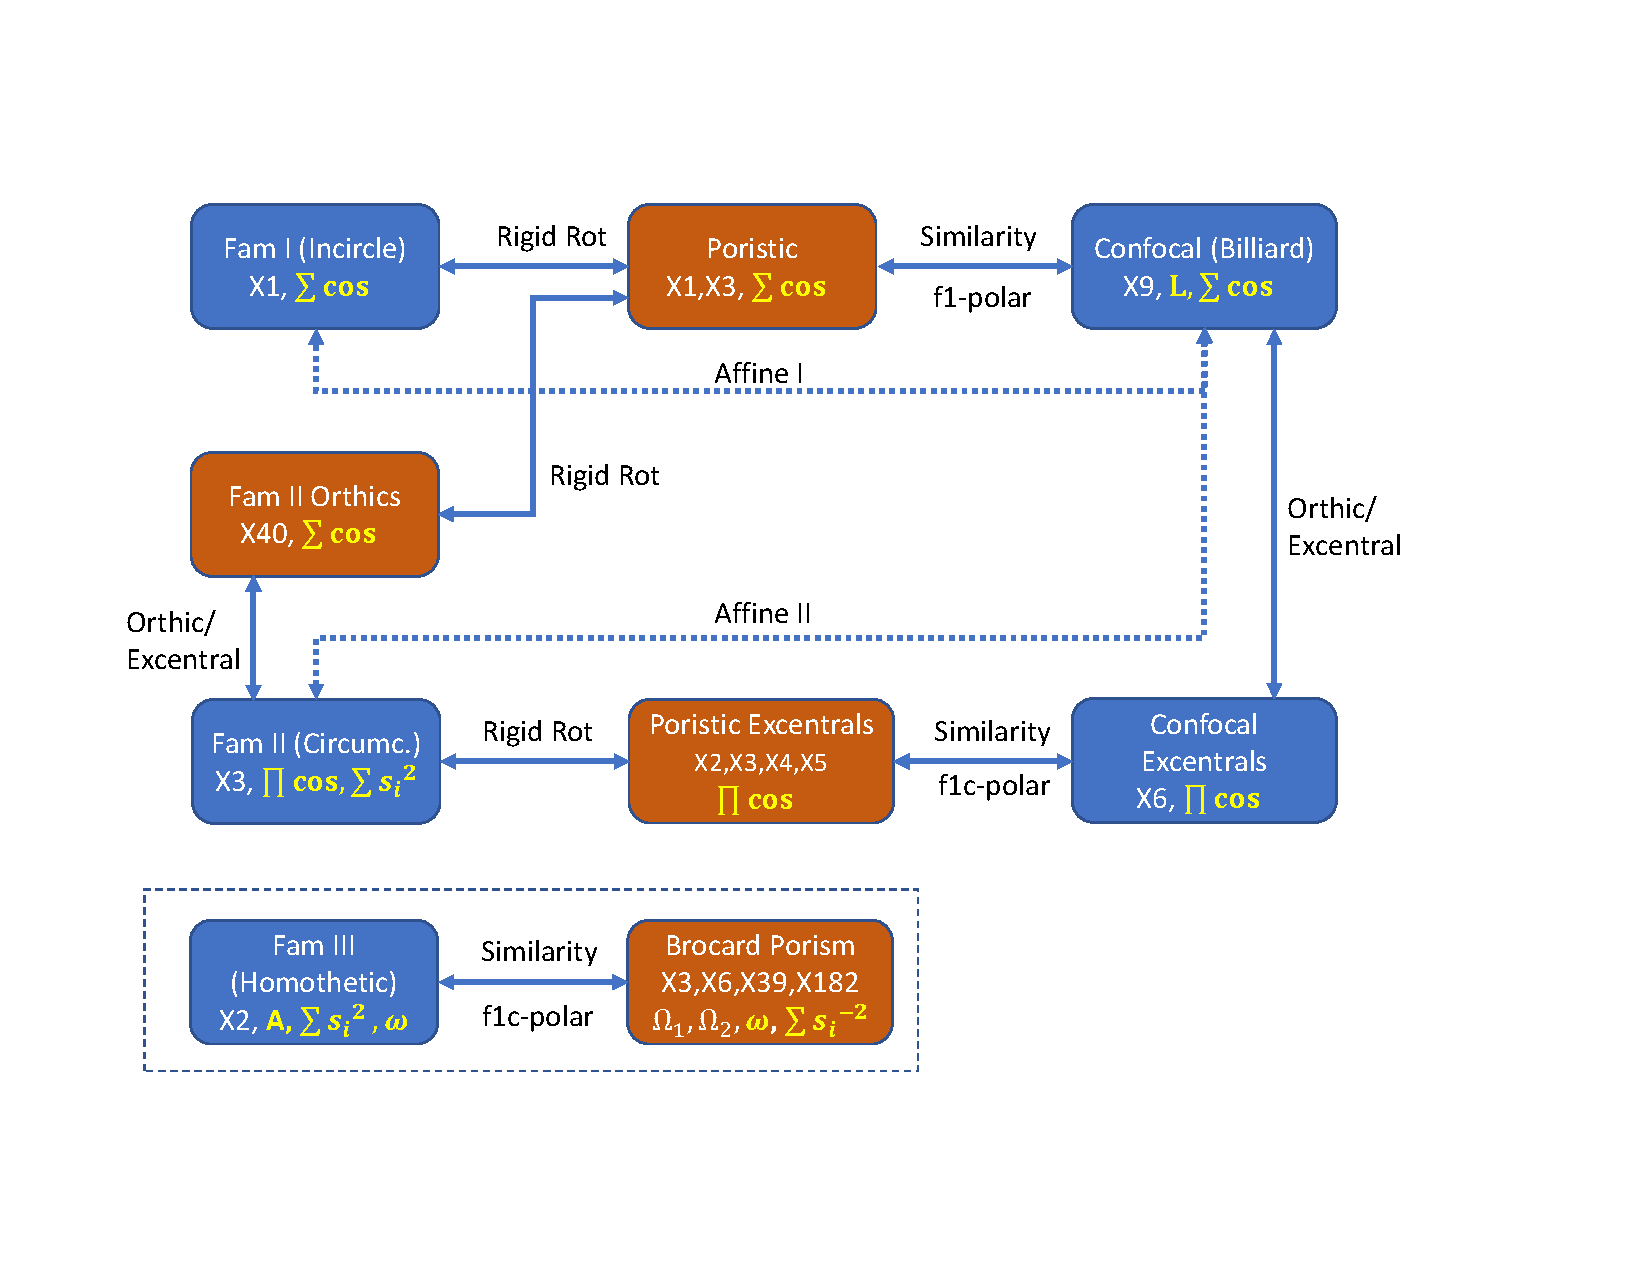
\includegraphics[trim={60 90 80 90},clip,width=\textwidth]{chap_03/pics/pics_03_250_poncelet_transformations.pdf}
  \caption{Families mentioned in this chapter (blue ones are concentric, tan ones are non-concentric), as well as the transformations under which certain families are interrelated.}
    \label{fig:03-transformations}
\end{figure}

\section{Exercises}

\begin{exercise}
Show that over the poristic family, the locus of the foci of the $X_9$-centered circumconic (the circumbilliard) is a circle.
\end{exercise}

\begin{exercise}
Prove \cref{prop:03-antiorthic}. Furthermore, prove the intersection point of $X_1 X_3$ with the antiorthic axis is the Schröder point $X_{1155}$.
\end{exercise}

\begin{exercise}
Prove that over the poristic family the inconic centered on $X_1$ is axis-parallel with the circumconic centered on $X_9$ (i.e., the circumbilliard), see this \href{https://youtu.be/0VHBjdHXbJc}{Video}.
\end{exercise}


\begin{exercise}
Recall the cosine circle $\Cm$ (also known as the second Lemoine circle) is centered on a triangle's symmedian point $X_6$. Let $\E'$ be the Brocard ellipse of some triangle $T$. Let $\beta$ be the aspect ratio of $\E'$, i.e., $a'/b'$. Show that for any $T$, above (resp. below) a certain $\beta$, $\Cm$ is tangent to $\E'$ at two distinct points (resp. it is exterior to $\E'$). See it \href{https://bit.ly/2RqhUQV}{Live}.
\end{exercise}


\begin{exercise}
Show that the poristic excentral family is also the polar image of billiard excentrals wrt to a circle centered on a billiard (i.e., the caustic) focus. See it \href{https://bit.ly/33c1s9A}{Live}.
\end{exercise}

\begin{exercise}
Show that over the Brocard porism the radius $r^*$ of the cosine circle is invariant.
\end{exercise}

\begin{exercise}
Show that the first Lemoine circle (centered on $X_{182}$ is stationary over the Brocard porism. Above a certain $a'/b'$, this circle is tangent to one of the minor vertices of the caustic. See it \href{https://bit.ly/3tp0XUq}{Live}.
\end{exercise}

\begin{exercise}
Ehrmann's ``third'' Lemoine circle is studied in \cite{darij2012-ehrmann}, centered on $X_{576}$, is defined as follows: for each vertex, consider the 3 circles containing pairs of vertices and the symmedian point $X_6$. The third Lemoine circle contains the 6 intersections of said circles (2 each) with the sidelines. Prove this circle is also stationary over the Brocard porism, i.e., all three Lemoine circles are; see it \href{https://bit.ly/3tw09gA}{Live}. 
\end{exercise}


\begin{exercise}
Prove the expression and inequality for $\cot{\omega}$ in \cref{prop:03-brocard-w}.
\end{exercise}

\begin{exercise}
That the Brocard axis $X_3 X_6$ is stationary over the Brocard porism is established. Prove that the Lemoine axis, which intersects the Brocard axis at the Schoutte point $X_{187}$, is also stationary; see it \href{https://bit.ly/3nTRi75}{Live}.
\end{exercise}

\begin{exercise}
The so-called ``second'' Brocard triangle, defined in \cite[Second Brocard Triangle]{mw}, has vertices at the intersections of symmedians (cevians through $X_6$) with the Brocard circle. Show that over the Brocard porism, the family of second Brocard triangles is a new, smaller Brocard porism which shares the isodynamic points $X_{15}$ and $X_{16}$ with the original family. Prove that if this is iterated, the shrinking porisms converge to $X_{15}$. See it \href{https://bit.ly/3ttMNBg}{Live}.
\end{exercise}

\section{Research Questions}

\begin{question}
Show that (i) the family of tangential triangles to the Brocard porism is also Ponceletian (caustic is the Brocard circumcircle).(ii) Derive the axes for the ellipse it is inscribed in.  and that (iii) its Gergonne point $X_7$ is stationary and coincides with the symmedian point $X_6$ of the Brocard porism; (iv) the locus of $X_{20}$ of the tangentials is a segment along the Brocard axis of the original family. \href{https://bit.ly/2RpNxdn}{Live} 
\end{question}

\begin{question}
The 3 Apollonius' circles of a triangle pass through a vertex and its two isodynamic points $X_{15}$ and $X_{16}$, see \cite[Isodynamic points]{mw}. Prove that over the Brocard porism, the sum of the inverse squared radii of the three Apollonius circles is invariant, see them \href{https://bit.ly/3elEzXI}{Live}.
\end{question}

\begin{question}
Prove that the polar image of the Brocard porism with respect to a circle centered on a caustic focus is another (tilted, smaller) Brocard porism whose Brocard inellipse shares a focus with the original one. Where does the sequence of Porisms converge? See it \href{https://bit.ly/3b7erOg}{Live}.
\end{question}

\section{Summary}
\label{sec:03-summary}
\begin{figure}
    \centering
    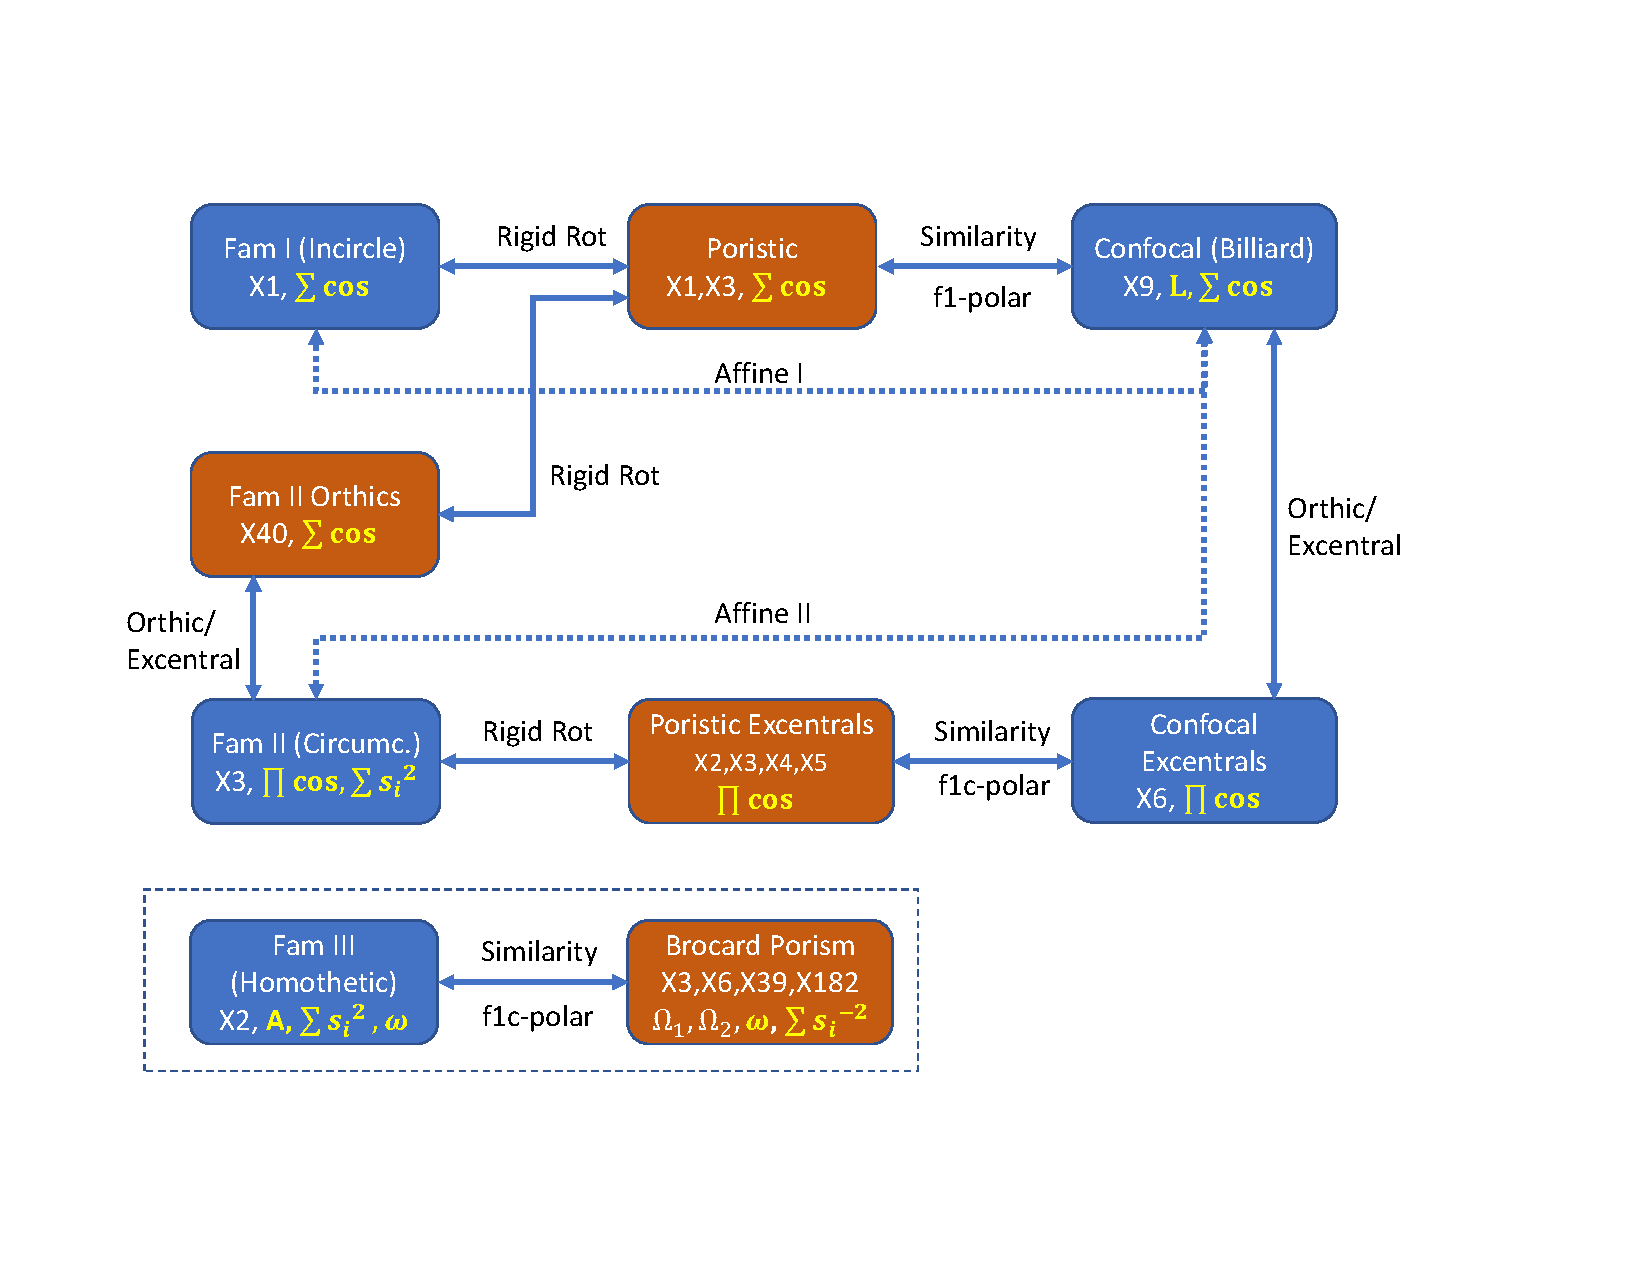
\includegraphics[width=\textwidth]{chap_03/pics/pics_03_250_poncelet_transformations.pdf}
    \caption{Caption}
    \label{fig:my_label}
\end{figure}

\section{Appendix: Vertex Parametrizations}
\label{sec:03-vtx-param}

\subsection{A generic CAP pair}

Consider a general pair of CAP ellipses denoted $\E$ and $\E_c$. We will derive a generic parametrization for the vertices of 3-periodics in such a pair. A first calculation will be helpful. Referring to \cref{fig:ell-ints}(left), the following are coordinates for the intersections $P_2$ and $P_3$ on $\E$ of the two tangents to $\E_c$ seen from a point $P_1=[x_1,y_1]$ also on $\E$:

\begin{figure}
    \centering
    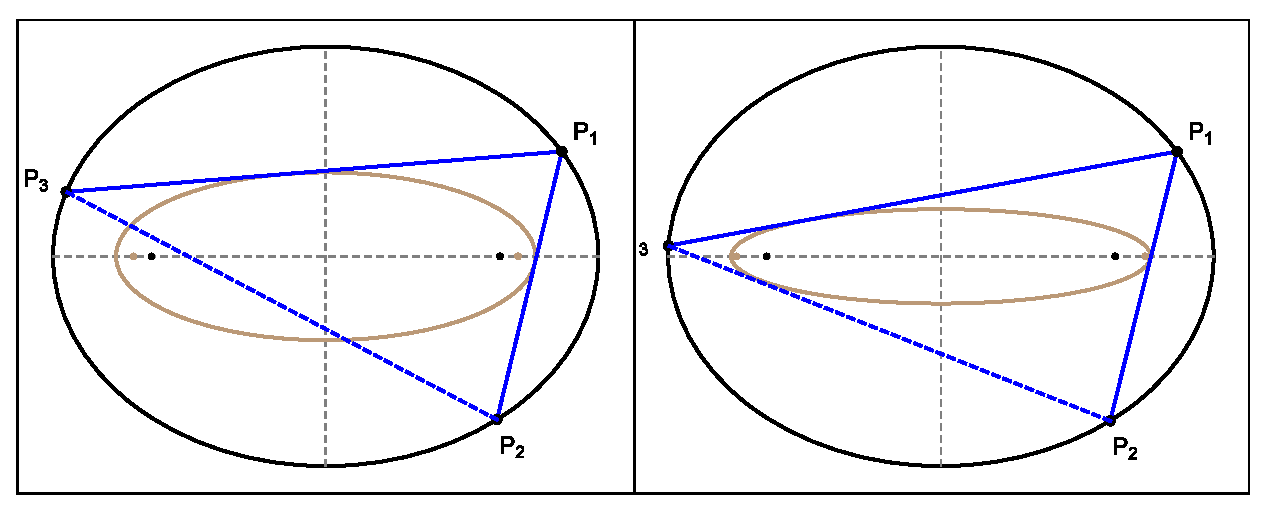
\includegraphics[width=\textwidth]{pics_03_070_ell_ints.eps}
    \caption{\textbf{Left:} Two CAP ellipses (black and brown), and a point $P_1$ on the outer one. The lines thru $P_1$ tangent to the inner ellipse intersect the outer one at $P_2$ and $P_3$. Notice that $P_2 P_3$ cut thru the inner ellipse, i.e., the pair of ellipses does not satisfy Cayley's conditions. \textbf{Right:} the minor axis of the inner ellipse has been scaled such that $P_1 P_2 P_3$ is now a Poncelet triangle.}
    \label{fig:ell-ints}
\end{figure}

\begin{align}
    P_2& =[x_2,y_2]=\frac{1}{k_2}\left[\frac{u_1 x_1 + u_2 y_1}{b} ,  \frac{w_1 x_1 + w_2 y_1}{a} \right] \label{eq:03-n3-conc-general} \\
    P_3&=[x_3,y_3]=\frac{1}{k_2}\left[\frac{w_1 x_1 - w_2 y_1}{b},\frac{w_1 x_1 - w_2 y_1}{a}\right] \nonumber
\end{align}
where:
\begin{align*}
    u_1 &=b\left(a^4  b_c^4 -(a^2 -  a_c^2)^2 b^4 \right) \\
    u_2 &= 2 a k_1 \left( (a^2 + a_c^2)b^2 - b_c^2 a^2\right) \\
    k_1&=\sqrt{ b^2  b_c^2 (a^2 -  a_c^2)  x_1^2 +  a_c^2 a^2(b^2 -  b_c^2)  y_1^2}\\
    k_2 &=\left(\frac{a^2 (b^2 +  b_c^2) - a_c^2 b^2 }{a}x_1\right)^2+ \left(\frac{a^2 (b^2 -  b_c^2) + a_c^2b^2 }{b} y_1\right)^2\\
    w_1&=2 b k_1\left( (b^2 +  b_c^2) a^2 - a_c^2 b^2\right) \\
    w_2&= a\left(a_c^4b^4-a^4(b^2-b_c^2)^2\right)
     %=-a (a^2( b^2 -    b_c^2) -  a_c^2 %b^2) (a^2 (b^2 -   b_c^2) +  a_c^2 b^2)
\end{align*}
 
\subsection{Brocard Porism}

Consider an isosceles Poncelet triangle $\Tm=ABC$ in the Brocard porism, where $AB$ is tangent to $\E$ at one of its minor vertices. Let $|AB|=2d$ and the height be $h$. Let $\zeta=d^2+h^2$. Let the origin $(0,0)$ be at its circumcenter $X_3$. Its vertices will be given by:

\[A=\left[-d ,\frac{d^2-h^2}{2h}\right], \;\;\; B= \left[d,\frac{d^2-h^2}{2h}\right], \;\;\; \left[0 ,\frac{\zeta}{2h}\right] \]


\begin{proposition}\label{prop:pair_brocard}
The Brocard porism containing $\Tm$ as a Poncelet triangle is defined by the following circumcircle $\K_0$ and Brocard inellipse $\E$:

\begin{align*}
\K_0:& x^2+y^2-R^2=0, \;\;\; R=\frac{\zeta}{2h}\\
\E:& -64d^2  h^4  x^2-4  h^2  (9  d^2+h^2)  \zeta  y^2 +4  h  (3  d^2+h^2)  (3  d^2-h^2)  \zeta  y\\&-(d^2-h^2) (9d^2 -h^2) \zeta^2=0
\end{align*}
\end{proposition}

\begin{proof}
The proof follows from $\Tm$, and isosceles Poncelet triangle. Recall that the Brocard inellipse is centered at $X_{39}$. Its perspector is $X_6$, i.e., it will be tangent to $\Tm$ where cevians through $X_6$ intersect it; see \cite[Brocard inellipse]{mw}.
\end{proof}


Consider the pair: circle $x^2+y^2=R^2=(d^2+h^2)^2/(4h^2)$ and   ellipse
$x^2/a^2+(y-y_0)^2/b^2=1$, with  semi-axes
 \[  (a,b)=\left(\frac{d\sqrt{d^2+h^2}}{9d^2+h^2},\frac{4d^2}{9d^2+h^2}\right)
    \]
and center $(0,y_0)$,  $y_0=(9d^4 - h^4)/(2h(9d^2  +  h^3))$.

Vertices $P_i=[x_i,y_i]$, $i=1,2,3$ of Brocard porism triangles are given by:

{\small  
\begin{equation}
    \aligned
    x_1 &= \cos{t}/q_1\\
    y_1 &= \sin{t}/q_1 \\
    x_2 &= -d (d^2 + h^2) ((3 d^2 + h^2)\sin{t} + 2d h \cos{t}- 3 d^2 + h^2)/q_2 \\
    y_2&=-(d^2 + h^2) ((9 d^4 - 2 d^2 h^2 + h^4)\sin{t} - 2 d h (3 d^2 + h^2)\cos{t} - 9 d^4 + h^4)/(2 b q_2) \\
    x_3 &= d (d^2 + h^2) (2 d h \cos{t} - (3 d^2 + h^2) \sin{t} + 3 d^2 - h^2)/q_3\\
    y_3 &=(d^2 + h^2) (2d h (3 d^2 + h^2) \cos{t}+ (9 d^4 - 2 d^2 h^2 + h^4)\sin{t} - 9 d^4 + h^4)/(2 b q_3) \\
    q_1&=(2h)/(d^2+h^2)\\
    q_2&= 2 d h (3 d^2 - h^2)\cos{t} - (9 d^4 - h^4) \sin{t}  + 9 d^4 + 2 d^2 h^2 + h^4\\
    q_3&= 2 d h (3 d^2 - h^2)\cos{t} + (9 d^4 - h^4)\sin{t} - 9 d^4 - 2 d^2 h^2 - h^4
\endaligned
\label{eqn:03-vertices-brocard}
\end{equation}
}


\section{Exercises}
\label{sec:03-exercises}
\begin{exercise}
\label{ex:03-circumbilliard} 
Show that every triangle has a circumbilliard, i.e., an ellipse to which it is inscribed and to which it is a billiard 3-periodic. Compute the axes of said circumbilliard with respect to triangle vertices. 
\end{exercise}
 
\begin{exercise}
 \label{ex:03-power-euler} 
Prove that the power of the circumcircle with with respect to the common center in each of the following 3-periodic families is constant and given by the listed expressions. (i) incircle: $-a_e b_e$; (ii) homothetic: $-({a_e^2+b_e^2})/{2}$, and (iii) excentral: $-a^2-b^2-2\delta$. 
\end{exercise}

%\begin{exercise}\label{ex:33} 
%The {\em cosine circle} (also known as the second Lemoine circle) \cite[Cosine Circle]{mw} of a triangle passes through 6 points: the 3 pairs of intersections of sides with lines drawn through the symmedian $X_6$ parallel to sides of the orthic triangle. Recall that the orthic vertices are the feet of altitudes. Its center is $X_6$ \cite[Cosine Circle]{mw}. If one takes the excentral triangle of a billiard orbit as the reference triangle,   its orthic is the orbit itself.

%Show that the cosine circle of the excentral triangle is invariant over the family of 3-periodic orbits. Its radius $r^*=(a^2-b^2)/\sqrt{2\delta-a^2-b^2}$ is constant and it is concentric and external to the elliptic billiard.
%\end{exercise}

\begin{exercise}
\label{ex:03-cosine-circle}
Prove the radius $r^*$ of the stationary cosine circle of the excentral family is larger than the major axis $a$ of its caustic. 
\end{exercise}

\begin{exercise}
Recall the cosine circle $\Cm$ (also known as the second Lemoine circle) is centered on a triangle's symmedian point $X_6$. Let $\E'$ be the Brocard ellipse of some triangle $T$. Let $\beta$ be the aspect ratio of $\E'$, i.e., $a'/b'$. Show that for any $T$, above (resp. below) a certain $\beta$, $\Cm$ is tangent to $\E'$ at two distinct points (resp. it is exterior to $\E'$). See it \href{https://bit.ly/2RqhUQV}{Live}.
\end{exercise}

\begin{exercise}
Show that over the Brocard porism the radius $r^*$ of the cosine circle is invariant.
\end{exercise}

\begin{exercise}
Show that the first Lemoine circle (centered on $X_{182}$ is stationary over the Brocard porism. Above a certain $a'/b'$, this circle is tangent to one of the minor vertices of the caustic. See it \href{https://bit.ly/3tp0XUq}{Live}.
\end{exercise}

\begin{exercise}
Ehrmann's ``third'' Lemoine circle is studied in \cite{darij2012-ehrmann}, centered on $X_{576}$, is defined as follows: for each vertex, consider the 3 circles containing pairs of vertices and the symmedian point $X_6$. The third Lemoine circle contains the 6 intersections of said circles (2 each) with the sidelines. Prove this circle is also stationary over the Brocard porism, i.e., all three Lemoine circles are; see it \href{https://bit.ly/3tw09gA}{Live}. 
\end{exercise}

\begin{exercise}
Show that over the poristic family, the locus of the foci of the $X_9$-centered circumconic (the circumbilliard) is a circle.
\end{exercise}

\begin{exercise}
Prove \cref{prop:03-antiorthic}. Furthermore, prove the intersection point of $X_1 X_3$ with the antiorthic axis is the Schöder point $X_{1155}$.
\end{exercise}

\begin{exercise}
Prove that over the poristic family the inconic centered on $X_1$ is axis-parallel with the circumconic centered on $X_9$ (i.e., the circumbilliard), see this \href{https://youtu.be/0VHBjdHXbJc}{Video}.
\end{exercise}

\begin{exercise}
A pair of circles uniquely defines a {\em pencil} of coaxial circles; see \cite[Limiting Points]{mw}. The pencil contains exactly two circles which degenerate to a point, known as {\em limiting points}. Derive the location of such points for the poristic pair obtained from the image of two confocal ellipses centered at $[0,0]$ and with axes $a,b$ and $a',b'$.
\end{exercise}

\begin{exercise}
Let $\ell_1,\ell_2$ be the limiting points of the two circles which are polar images of a confocal pair $\E,\E'$ with respect to a circle centered on $f_1$. At what aspect ratio $a/b$ of $\E$ will $\ell_2$ coincide with $f_2$?
\end{exercise}

\begin{exercise}
A well-known result is that the inversion of a circle pair $\Cm,\Cm'$ with respect to a circle $\Cm_1$ centered on $\ell_1$ (resp. $\Cm_2$ centered on $\ell_2$) is a pair of concentric circles $\Cm_1'$ and $\Cm_1''$ (resp. $\Cm_1'$ and $\Cm_1''$). Prove the following lesser known result: the ratio of radii between $\Cm_1'$ and $\Cm_1''$ is the same as the ratio between $\Cm_2'$ and $\Cm_2''$. 
\end{exercise}


\begin{figure}
    \centering
    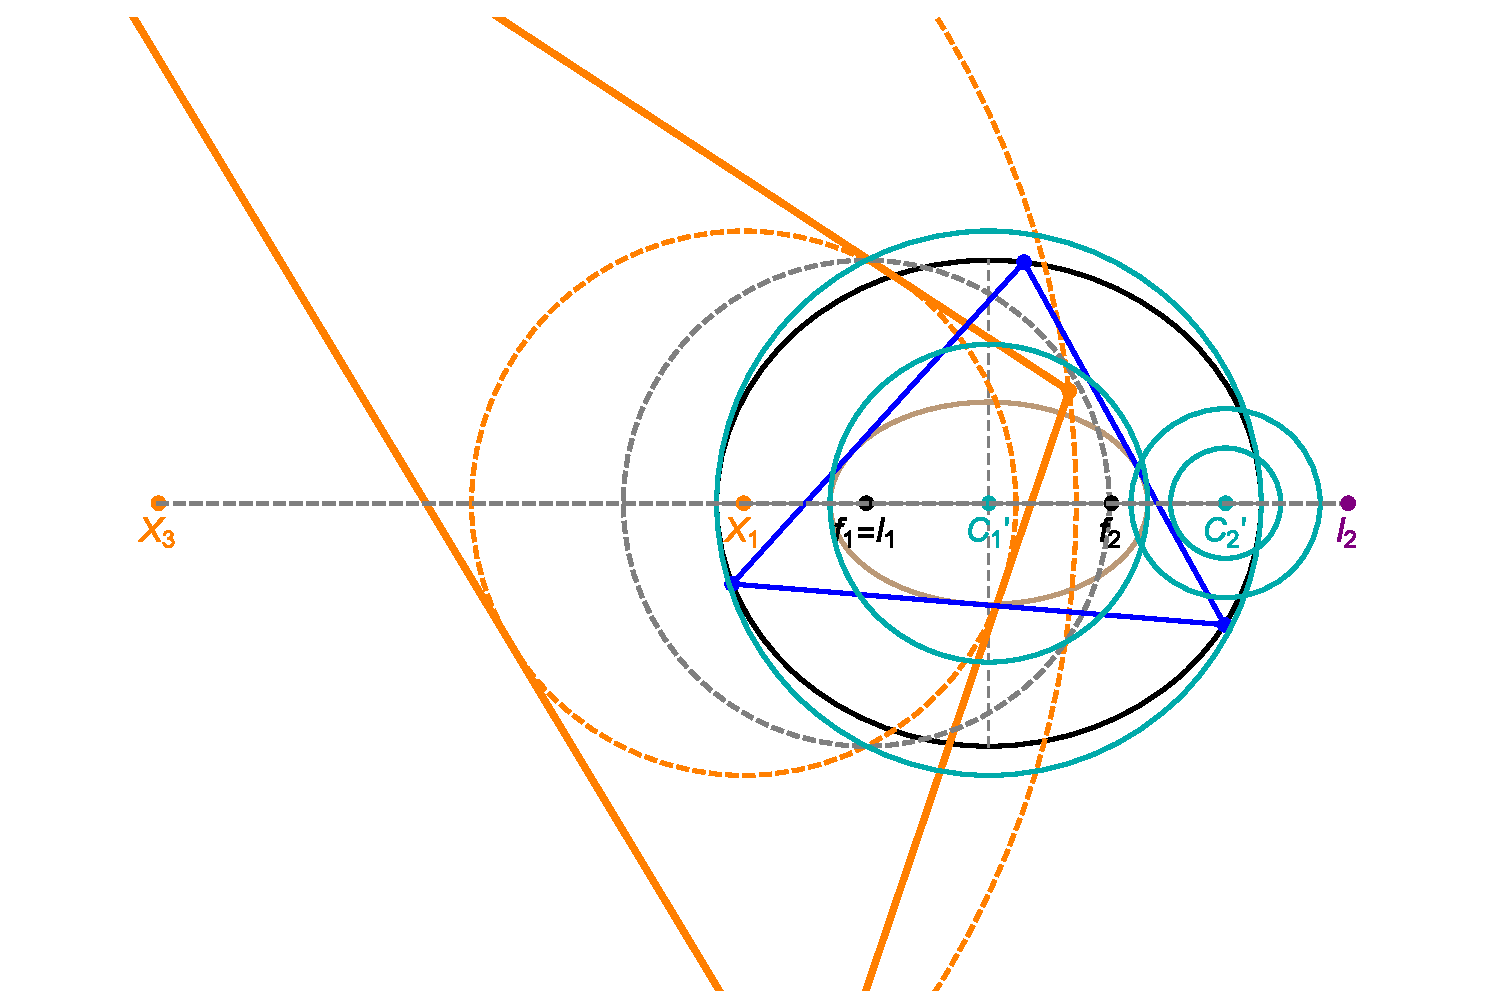
\includegraphics[width=.8\textwidth]{pics_03_210_concentric_inverted_pairs.eps}
    \caption{Concentric circle pairs (light blue) which are the inversions of the circumcircle and incircle (dashed orange) of the bicentric family  (blue) with respect to its two limiting point $\ell_1$ and $\ell_2$. Also shown are Billiard 3-periodics (blue) in the polar pre-image with respect to a circle (dashed gray) -- centered on $f_1=\ell_1$.}
    \label{fig:03-concentric-inverted}
\end{figure}

\begin{exercise}
Referring to \cref{fig:03-concentric-inverted}, let $\Cm,\Cm'$ be the pair of circles which are the polar image of a confocal pair of ellipses $\E,\E'$. Let $\Cm_1', \Cm_1''$ be the inversive images of $\Cm,\Cm'$ wrt to a cirlce centered on a focus of the ellipse pair. Prove that: (i) $\Cm_1'$ and $\Cm_1''$ are concentric with the ellipse pair and (ii) $\Cm_1'$ (resp. $\Cm_1''$) is externally tangent to $\E$ (resp. $\E'$) at its left and right major vertices.
\end{exercise}

\begin{exercise}
Prove \cref{lem:03-circum-x5-locus}.
\label{ex:03-circum-x5-locus}
\end{exercise}

\begin{exercise}
Recall the dual family has stationary orthocenter $X_4$. Prove that the inversive image of the dual family wrt to a circle concentric with the ellipse pair is a non-Ponceletian family with incenter $X_1'$ stationary at the common center. This inversive family is inscribed in Booth's curve and its caustic can contain multiple spikes; see it \href{https://bit.ly/3vCCe05}{Live}.
\end{exercise}

\begin{exercise}
Prove the inversive image of billiard 3-periodics with respect to a focus-centered circle is a non-Ponceletian family inscribed in Pascal's Limaçon whose Gergonne point $X_7$ is stationary; see it \href{https://bit.ly/3edwKD7}{Live}. Indeed, this family has constant perimeter (to be shown later).
\end{exercise}

\begin{exercise}
Show that the poristic excentral family is also the polar image of billiard excentrals wrt to a circle centered on a billiard (i.e., the caustic) focus. See it \href{https://bit.ly/33c1s9A}{Live}.
\end{exercise}

\begin{exercise}
Prove the expression and inequality for $\cot{\omega}$ in \cref{prop:03-brocard-w}.
\end{exercise}

\begin{exercise}
That the Brocard axis $X_3 X_6$ is stationary over the Brocard porism is established. Prove that the Lemoine axis, which intersects the Brocard axis at the Schoutte point $X_{187}$, is also stationary; see it \href{https://bit.ly/3nTRi75}{Live}.
\end{exercise}

\begin{exercise}
The so-called ``second'' Brocard triangle, defined in \cite[Second Brocard Triangle]{mw}, has vertices at the intersections of symmedians (cevians through $X_6$) with the Brocard circle. Show that over the Brocard porism, the family of second Brocard triangles is a new, smaller Brocard porism which shares the isodynamic points $X_{15}$ and $X_{16}$ with the original family. Prove that if this is iterated, the shrinking porisms converge to $X_{15}$. See it \href{https://bit.ly/3ttMNBg}{Live}.
\end{exercise}

\section{Research Questions}
\label{sec:03-research}
\begin{question}
Referring to \cref{fig:03-n3-dual}, are there any conserved quantities for the dual family besides stationarity of $X_4$ at the common center?
\end{question}

\begin{question}
Referring to  the dashed green triangle in \cref{fig:03-n3-affine}(middle), are there any conserved quantities and/or fixed triangle centers for the family which is an $s$-affine image of billiard excentrals?
\end{question}

\begin{question}
Consider the family of inversive images of excentral triangles with respect to a circle centered at a point $M$ in the plane. Show the symmedian point $X_6$ of such a family will be stationary regardless of $M$. Compute the location of $X_6$. See this curious phenomenon in a \href{https://youtu.be/wwX_QfkjVi0}{Video}.
\end{question}


\chapter{Non-concentric, Axis-Parallel (NCAP)}
\label{chap:04-n3-ncap}
\section{Introduction}
\begin{itemize}
    \item confocal
    \begin{itemize}
        \item loci of incenter, excenters
        \item loci of intouchpoints
        \item loci od X1,X2,X3,X4,X5
        \item loci of X11 and X100
        \item loci of derived triangle vertices: extouch (caustic), intouch (sextic), feuerbach triangle, medial, anticomplementary 
    \end{itemize}
    \item brocard points
\end{itemize}

\section{Loci of Billiard 3-Periodics}
\section{Introduction}

In this section we will tour some phenomena concerning the loci of triangle centers over elliptic billard 3-periodics, including the loci of vertices of certain derived triangles.

Recall the loci of the incenter $X_1$ and excenters (vertices of the excentral family) were previously shown to be ellipses, see \cref{sec:03-inc-exc-loci} and \cref{fig:billiard-grid}. Recall also that the locus of the Mittenpunkt $X_9$ is a point, see \cref{sec:03-stationary}.

\begin{itemize}
\item confocal
    \begin{itemize}
        \item loci of incenter, excenters
        \item loci of intouchpoints
        \item loci od X1,X2,X3,X4,X5
        \item loci of X11 and X100
        \item loci of derived triangle vertices: extouch (caustic), intouch (sextic), feuerbach triangle, medial, anticomplementary 
    \end{itemize}
    \item brocard points
\end{itemize}

We will omit most proofs etc.

\section{Loci of the first five Kimberling centers}

The semi-axes $a_1,b_1$ for the elliptic locus of the incenter $X_1$ were given in \cref{thm:03-incenter-excenter}. It turns the loci of the next four centers in \cite{etc} are also ellipses. There are the barycenter $X_2$, the circumcenter $X_3$, the orthocenter $X_4$, and the center of the 9-point circle (also known as Euler's circle) $X_5$. Their semi-axes are given by:

\begin{align*}
    \left(a_2,b_2\right)=&k_2\left(a,b\right),\;\text{with}\; k_2=\frac{2\delta -a^{2}-b^{2}}{3c^2}\\
     \left(a_3,b_3\right)=&\left(\frac{a^{2}-\delta}{2a},\frac{\delta-b^{2}}{2b}\right)\\
 \left(a_4,b_4\right)=&\left(\frac{k_4}a,\frac{k_4}b\right),\;\text{with}\;k_4=\frac{  (a^{2}+b^{2})\delta-2\,a^{2}b^{2} }{c^2}\\
   \left(a_5,b_5\right)=&\left(\frac{- w'_5(a,b)+ w''_5(a,b) \delta}{ w_5(a,b)},\;\frac{ w'_5(b,a)-{w''_5(b,a) \delta}}{w_5(b,a)}\right)
\end{align*}
where $w'_5(u,v)=u^2(u^2+3v^2)$, $w''_5(u,v)=3u^2+ v^2$, and $w_5(u,v)=4u(u^2-v^2)$. Note that (i) $a_2/b_2=a/b$ and (ii) $b_4/a_4=a/b$.

As it turns out, the locus of 49 out of the first 200 centers in \cite{etc} are ellipses. These are: $X_k$, $k=$1,  2,  3,  4,  5,  7,  8,  10,  11,  12,  20,  21,  35,  36,  40,  46,  55,  56,  57,  63,  65,  72,  78,  79,  80,  84,  88,  90,  100,  104,  119,  140,  142,  144,  145,  149,  153,  162,  165,  190,  191,  200. Links to live animations as well as expressions for their semi-axes are provided in \cite{garcia2021-ellipses-web}.

%% Swans
%% the following centers lie on the $X_9$-centered circumellipse: 88, 100, 162, 190 \cite{etc}.

\begin{figure}
\centering
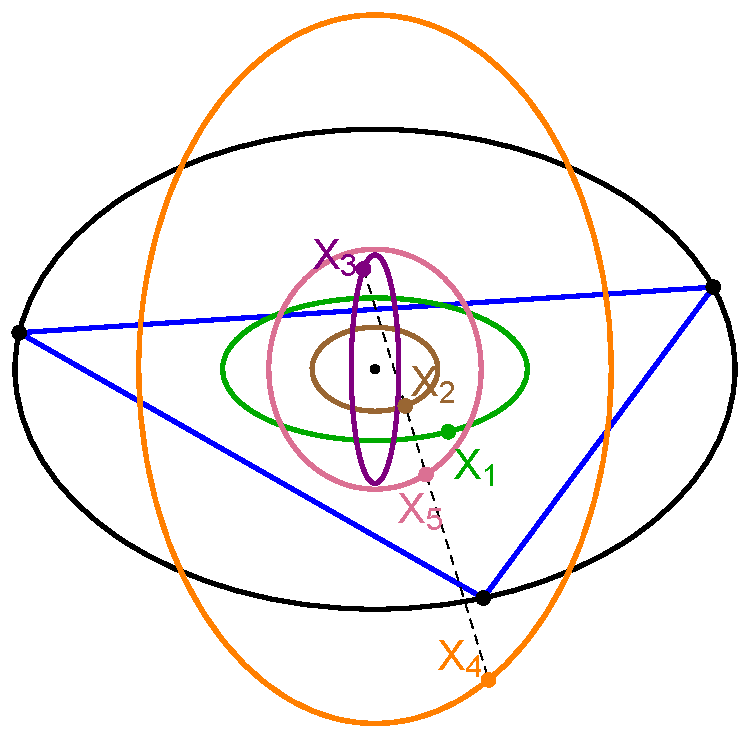
\includegraphics[width=.6\textwidth]{pics_04_060_locus_x12345.pdf}
\caption{Over billiard 3-periodics, the loci of incenter $X_1$, barycenter $X_2$, circumcenter $X_3$, orthocenter $X_4$, and 9-point center $X_5$ are all ellipses. The Euler line (dashed black) is shown passing through all but the first center. \href{https://youtu.be/sMcNzcYaqtg}{Video}, \href{https://bit.ly/3eVScgE}{Live}}
\label{fig:04-x12345}
\end{figure}

%%% begin X4
\section{The locus of the orthocenter: when 3-periodics are obtuse}

\begin{figure}
    \centering
    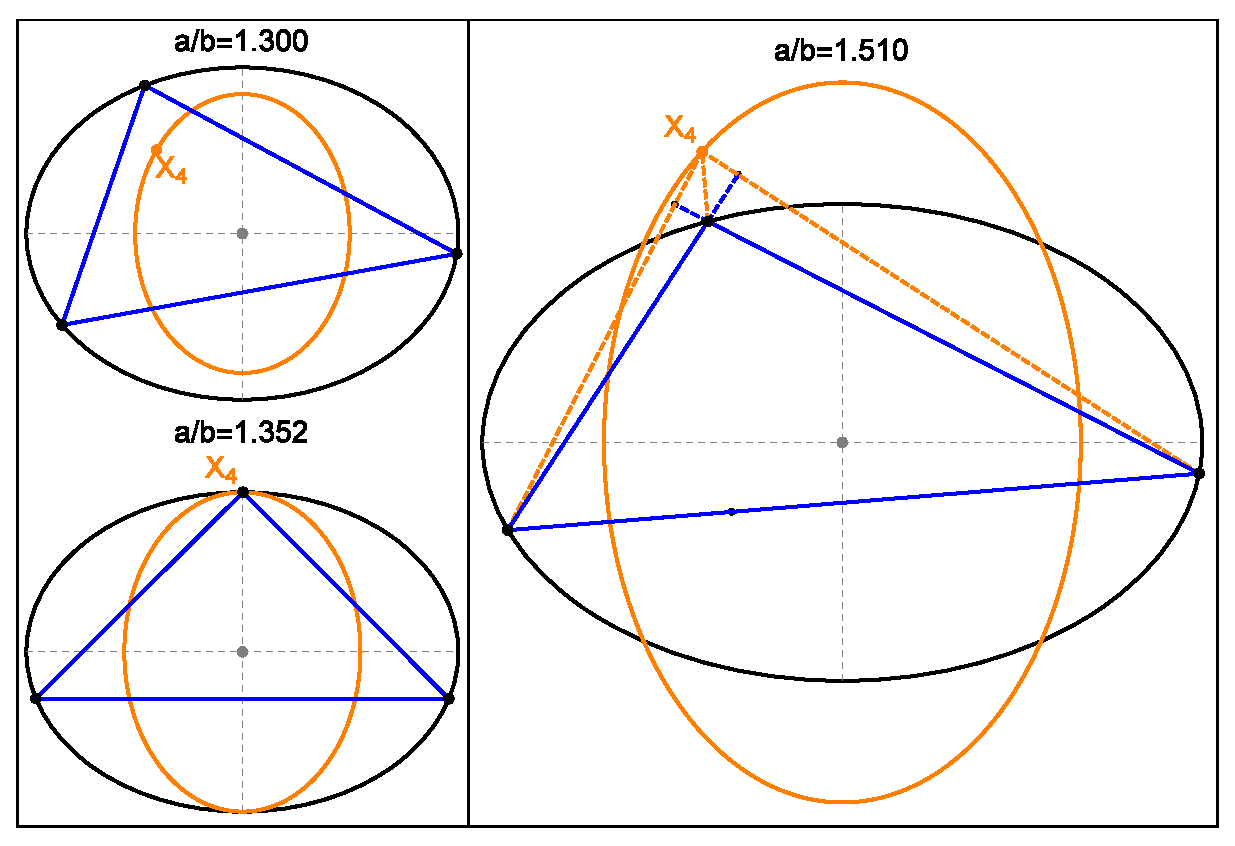
\includegraphics[width=\textwidth]{pics_04_130_ort_loci.eps}
    \caption{Locus of the orthocenter (orange) over elliptic billiards with different aspect ratios. If $a/b$ is (i) less than (resp. (ii) equal, (iii) greater than) $\alpha_4{\simeq}1.352$, the locus of the orthocenter $X_4$ (orange) is (i) interior (resp. (ii) internally tangent, (iii) intersecting) with the elliptic billiard. In (i) and (ii) all 3-periodics are acute, whereas in (iii) some will be obtuse.}.
    \label{fig:04-orthocenter-loci}
\end{figure}

It turns out the locus of $X_4$ can be used to determine if the billiard 3-period family will contain obtuse triangles. Referring to Figure~\ref{fig:04-orthocenter-loci}:

\begin{proposition}
The locus of $X_4$ is internally tangent to the elliptic billiard at its top and bottom vertices when $a/b=\alpha_4$ given by:

\[\alpha_4 = \sqrt{2\,\sqrt {2}-1}\;{\simeq}\;1.352.\]
\label{prop:04-alpha4}
\end{proposition}

\begin{proof}
The equation $b_4=b$ is equivalent to $a^4+2a^2b^2-7b^4=0.$ Therefore, as $a>b>0$, it follows that $a/b=\sqrt{2\,\sqrt {2}-1}.$
\end{proof}

\noindent Let $\alpha_4^*$ be the positive root of
${x}^{6}+{x}^{4}-4\,{x}^{3}-{x}^{2}-1=0$, i.e.,
$\alpha_4^{*}={\simeq}\;1.51$. 

\begin{proposition}
When $a/b=\alpha_4^{*}$, then $a_4=b$ and $b_4=a$, i.e., the locus of $X_4$ is identical to a rotated copy of Billiard. 
\end{proposition}

\begin{proof}
The condition $a_4=b$, or equivalently $b_4=a$, is defined by $a^6+a^4b^2-4a^3b^3-a^2b^4-b^6=0$. Graphic analysis shows that ${x}^{6}+{x}^{4}-4\,{x}^{3}-{x}^{2}-1=0$ has only one positive real root which we call $\alpha_4^*$.
\end{proof}

\begin{theorem}
If $a/b<\alpha_4$ (resp. $a/b>\alpha_4$) the 3-periodic family will not (resp. will) contain obtuse triangles.
\end{theorem}

\begin{proof}
If the 3-periodic is acute, $X_4$ is in its interior, therefore also internal to the EB. If the 3-periodic is a right triangle, $X_4$ lies on the right-angle vertex and is therefore on the EB. If the 3-periodic is obtuse, $X_4$ lies on exterior wedge between sides incident on the obtuse vertex (feet of altitudes are exterior). Since the latter is on the EB, $X_4$ is exterior to the EB.
\end{proof}
%%% end X4

%%% begin X6
\section{Quartic locus of the symmedian point \torp{$X_6$}{X(6)}}
\label{sec:symmedian}

The symmedian point $X_6$ is replete with properties, indeed it is known as the crown jewel of triangle geometry \cite[Symmedian Point]{mw}. Its construction is deceptively simple: the point where a triangle's {\em symmedians} concur; these are reflections of medians on the bisectors. Its trilinear coordinates could not be simpler: $[a:b:c]$. However, it is the first Kimberling center whose locus over billiard 3-periodics is {\em not} an ellipse. 

In fact, when $1<a/b<2$, its locus is visually indistinguishable from a true ellipse; see Figure~\ref{fig:04-locus-x6}. Fortunately, its fit error is easily detectable with numerical methods. Indeed:

\begin{proposition}
The locus of $X_6$ is a convex quartic given by:

\begin{equation*}
  \X_6(x,y)=c_1 x^4+c_2 y^4+c_3 x^2 y^2+ c_4 x^2 + c_5 y^2 = 0
\end{equation*}

\noindent where:
$$
\begin{array}{rlrl}
c_1=&b^4(5\delta^2-4(a^2-b^2)\delta -a^2 b^2)&c_2=&a^4(5\delta^2+4(a^2-b^2)\delta-a^2b^2) \\
c_3=&2a^2 b^2(a^2 b^2+3\delta^2)&c_4=&a^2 b^4(3 b^4+2(2 a^2-b^2)\delta-5\delta^2)\\
c_5=&a^4 b^2(3 a^4+2(2 b^2-a^2)\delta-5\delta^2)&\delta=&\sqrt{a^4-a^2 b^2+b^4}
\end{array}
$$
\end{proposition}

\begin{proof}
Using a CAS, obtain symbolic expressions for the coefficients of a quartic symmetric about both axes (no odd-degree terms), passing through 5 known-points. Still using a CAS, verify the symbolic parametric for the locus satisfies the quartic.
\end{proof}

 \noindent Note the above is also satisfied by a degenerate level curve $(x,y)=(0,0)$, which we ignore.

\begin{remark}
We term the ``best-fit'' ellipse $\mathcal{E}_6$ the one internally-tangent to $\X_6(x,y)=0$ at its four vertices. Its semi-axes are given by: 

{\small  
\begin{align*}
%a_6=&\frac{\left[(3\,a^2-b^2)\delta %-(a^2+b^2)b^2\right]a}{a^4+b^4+2\delta^2}\nonumber\\
a_6= \frac{\left[(3\,a^2-b^2)\delta -(a^2+b^2)b^2\right]a}{a^2b^2+3\delta^2},\;\;\;
b_6= \frac{\left[(a^2-3\,b^2)\delta + (a^2+b^2)a^2\right]b}{a^2b^2+3\delta^2}
\label{eqn:x6-ellipse}
\end{align*}
}
\end{remark}

Table~\ref{tab:quartic-coeffs} shows the above coefficients numerically for a few values of $a/b$.

\begin{table}
    \centering
$$
\begin{array}{|c|c|c|c|c|c|c|c|}
\hline
 \text{a/b} & a_6 & b_6 & c_1/c_3 & c_2/c_3 & c_4/c_3 & c_5/c_3 & A(\mathcal{E}_6)/A(\mathcal{X}_6) \\
 \hline
  1.25 & 0.433 & 0.282 & 0.211 & 1.185 & -0.040 & -0.095 & 0.9999 \\
 1.50 & 0.874 & 0.427 & 0.114 & 2.184 & -0.087 & -0.399 & 0.9998 \\
 2.00 & 1.612 & 0.549 & 0.052 & 4.850 & -0.134 & -1.461 & 0.9983 \\
 3.00 & 2.791 & 0.620 & 0.020 & 12.423 & -0.157 & -4.769 & 0.9949 \\
 \hline
\end{array}
$$
\caption{Coefficients $c_i/c_3$, $i=1,2,4,5$ for the quartic locus of $X_6$ as well as the axes $a_6,b_6$ for the best-fit ellipse, for various values of $a/b$. The last-column reports the area ratio of the internal ellipse $\mathcal{E}_6$ (with axes $a_6,b_6$) to that of the quartic locus $\mathcal{X}_6$, showing an almost exact match.}
\label{tab:quartic-coeffs}
\end{table}


\begin{figure}
    \centering
    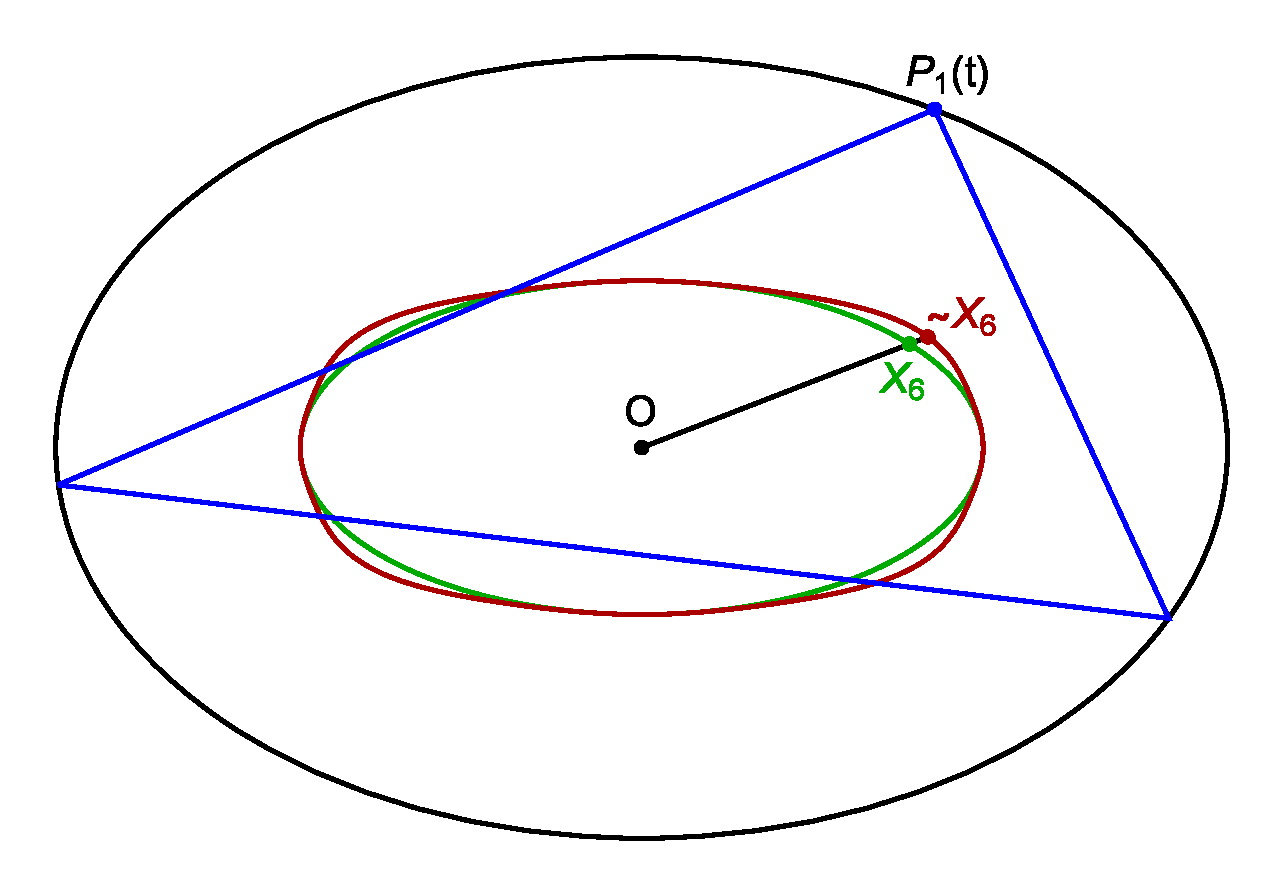
\includegraphics[width=.7\textwidth]{pics_04_090_symmedian.eps}
    \caption{Over billiard 3-periodics (blue), the locus of the symmedian point $X_6$ is a quartic (green). At the billiard aspect ratio shown, it is visually identical to an ellipse. Also shown is a copy of the quartic (red) such that the distance to a best-fit ellipse (green) is scaled 1000 fold. \href{https://bit.ly/3hxOZoV}{Live}}
    \label{fig:04-locus-x6}
\end{figure}
%%% end X6

%%% BEGIN X11 and X100
\begin{figure}
    \centering
    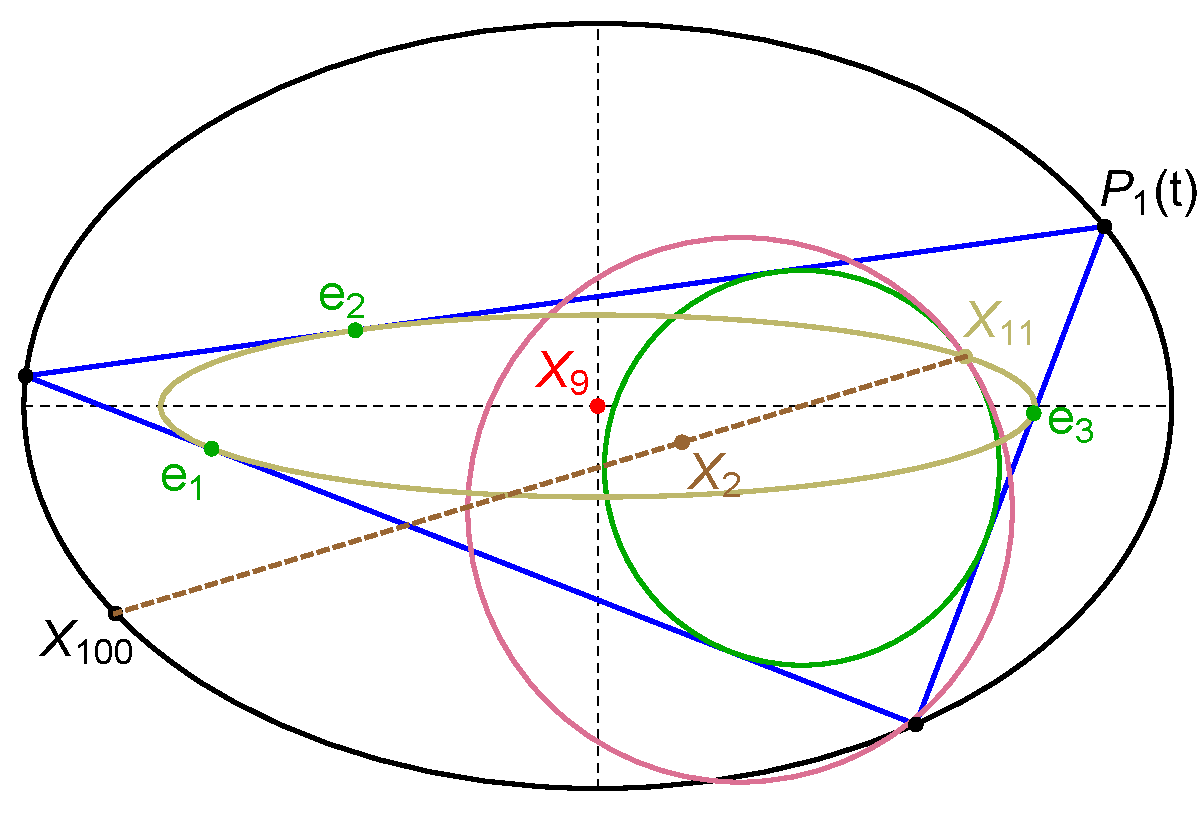
\includegraphics[width=.7\textwidth]{pics_04_080_feuerbach_loci.pdf}
    \caption{A billiard 3-periodic (blue). Also shown are the incircle (green) and 9-point circle (pink) which touch at the Feuerbach point $X_{11}$. Also shown is the latter's {\em anticomplement} $X_{100}$, and the three extouchpoints $e_1,e_2,e_3$. Over the billiard family, $X_{100}$ sweep the billiard while both $X_{11}$ and the extouchpoints sweep the caustic (though in opposite directions).
    % done
    \href{https://youtu.be/TXdg7tUl8lc}{Video},
    \label{fig:04-feuer-loci} \href{https://bit.ly/2S2LVqp}{Live}}
\end{figure}

\section{The locus of the Feuerbach point and its anticomplement}

Referring to \cref{fig:04-locus-x11-x100}, the Feuerbach point $X_{11}$ is the single point of contact between incircle and 9-point circle \cite[X(11)]{mw}. $X_{11}$ is known to lie on the $X_{9}$-centered inconic, i.e., the  Mandart inellipse \cite[Mandart inellipse]{mw}. Since the latter is unique:

\begin{observation}
The confocal caustic is the stationary Mandart inellipse of billiard 3-periodics.
\end{observation}

Therefore:

\begin{proposition}
Over billiard 3-periodics, $X_{11}$ sweepts the confocal caustic.
\end{proposition}

The anticomplement of a point $P$ is its double-length reflection about the barycenter $X_2$, i.e., $A(P) = X_2+2 X_2-P$. Stille referring,  \cref{fig:04-locus-x11-x100}, $X_{100}$ is the anticomplement of $X_{11}$. This point is known to lie on (i) the circumcircle, (ii) the Steiner circumellipse (centered on $X_2$), and most relevantly here, (iii) on the $X_9$-centered circumellipse \cite[X(9)]{etc}. Since the latter is unique:

\begin{observation}
The elliptic billiard is the stationary $X_9$-centered circumconic of billiard 3-periodics.
\end{observation}

Therefore:

\begin{proposition}
Over billiard 3-periodics, the locus of $X_{100}$ is the elliptic billiard.
\end{proposition}

The vertices of the so-called {\em extouch triangle} are the points of contact of the excircles with a triangle's sidelines \cite[Extouch triangle]{mw}. These are also known as {\em extouchpoints}. A known fact is that the Mandart inellipse (i.e., the caustic) touches a triangle's sidelines at the extouchpoints \cite[Mandart inellipse]{mw}. Therefore:

\begin{proposition}
Over billiard 3-periodics, the locus of the extouchpoints is the confocal caustic.
\end{proposition}

This is also illustrated in \cref{fig:04-locus-x11-x100}. A curious dynamic phenomenon is that while the extouchpoints follow the direction of motion of billiard 3-periodics along the outer ellipse (e.g., counter- or clockwise), $X_{11}$ rotates in the opposite direction; see this \href{https://bit.ly/2S2LVqp}{Live}.


%%% END X11 and X100

\section{Locus of vertices of some derived triangles}

A few triangles derived from billiard 3-periodics are shown in \cref{fig:04-derived-isosceles}. For their definitions see \cite{app:app-triangle} and \cite{mw}.

\begin{figure}
    \centering
    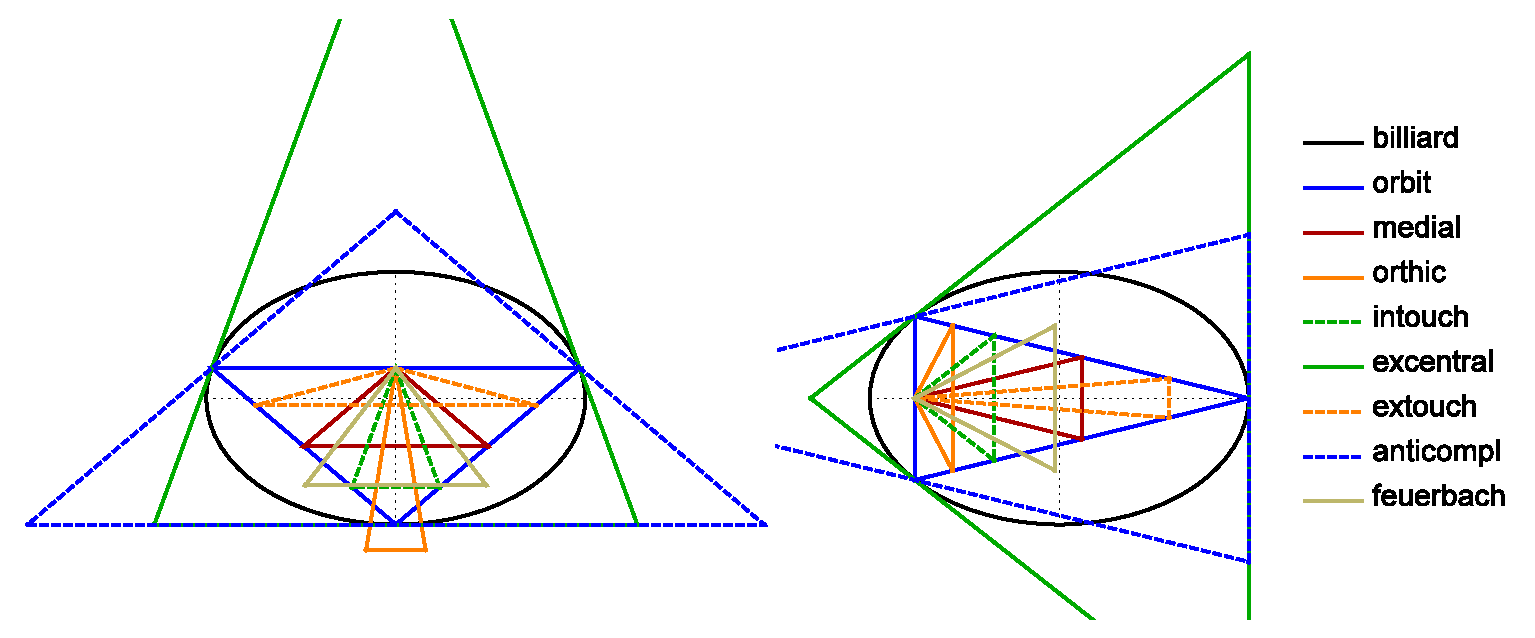
\includegraphics[width=\textwidth]{pics_04_100_confocal_derived.eps}
    \caption{Triangles derived from an isosceles billiard 3-periodic (blue). These contain one vertex on the axis of symmetry. \href{https://youtu.be/xyroRTEVNDc}{Video}}
    \label{fig:04-derived-isosceles}
\end{figure}

Mentioned in \cref{sec:01-introduction} was an early experiment which showed that over billiard 3-periodics, the locus of the vertices of the intouch triangle (i.e., the intouchpoints) is a 2-lobed, self-intersect curve; see \cref{fig:01-intouch-x59}.

As shown in \cref{fig:04-locus-x11-x100}, the loci of vertices of some other triangles derived from billiard 3-periodics aren't ellipses. A noteworthy exception is the extouch triangle, mentioned above.

\begin{figure}
    \centering
    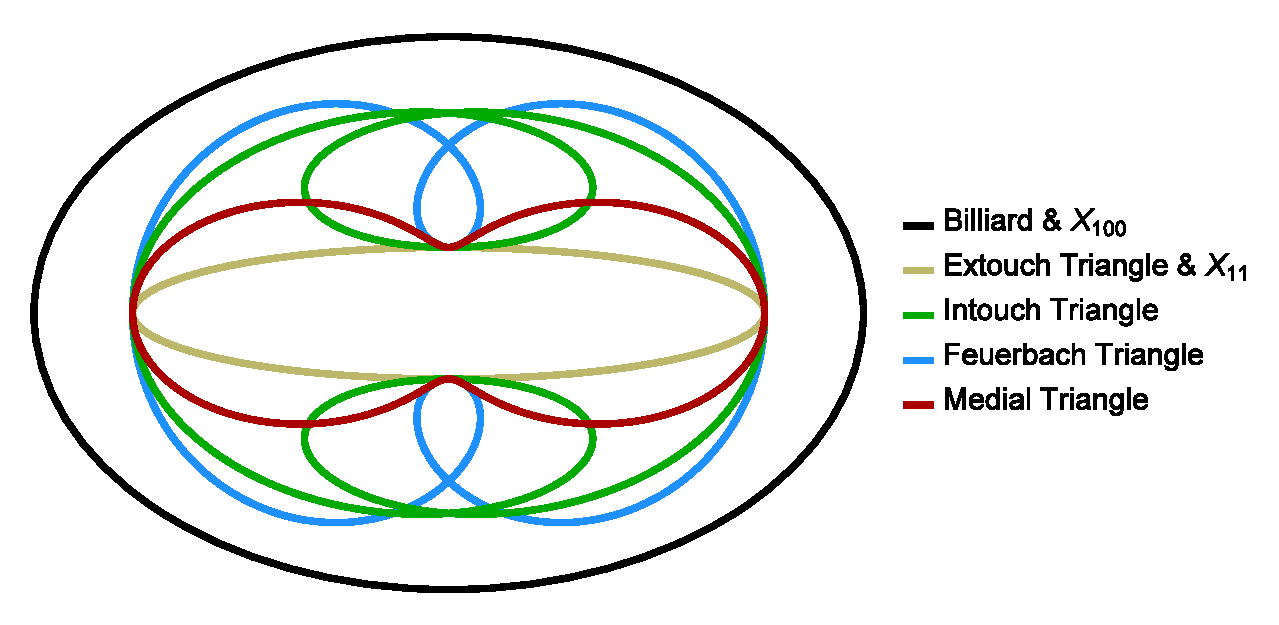
\includegraphics[width=\textwidth]{pics_04_070_non_elliptic.eps}
    \caption{Non-elliptic loci of the vertices of triangles derived from billiard 3-periodics: the (i) intouch (green), (ii) Feuerbach (not to be confused with the Feuerbach {\em point}) (blue), (iii) medial (red), triangles. A noteworthy excpetion is the extouch triangle (light brown), whose vertices sweep the confocal caustic.
     \href{https://youtu.be/OGvCQbYqJyI}{Video}, \href{https://bit.ly/3orrSxQ}{Live}}
    \label{fig:04-locus-x11-x100}
\end{figure}

\section{Orthic incenter: a locus with kinks}

Loci considered thus far have been smooth, regular curves. Here we give an example of one with four sharp corners. Recall the {\em orthic triangle} has vertices at the feet of a triangle's altitudes; see \cref{fig:04-orthic-incenter}. 

\begin{figure}
    \centering
    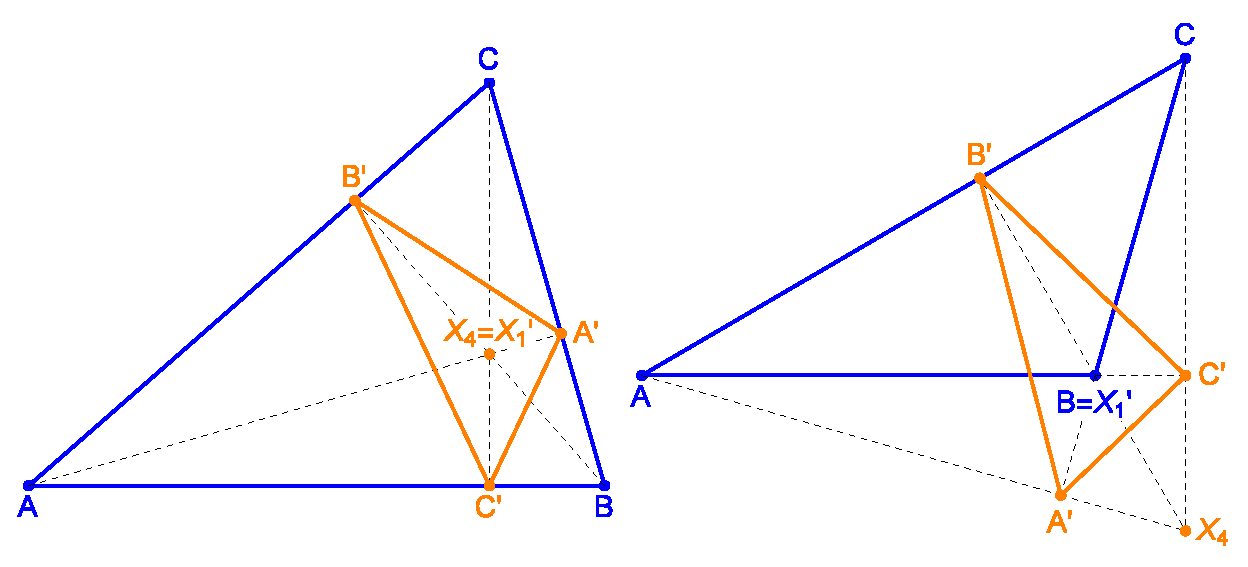
\includegraphics[width=.8\textwidth]{pics_04_140_orthic_incenter.eps}
    \caption{\textbf{Left}: the orthic triangle (orange) is shown of an acute reference triangle $T$ (blue), for with an interior orthocenter $X_4$. In this case, the orthic incenter $X_1'$ coincides with $X_4$. \textbf{Right}: When $T$ (blue) is obtuse, $X_4$ is exterior. Furthermore, two orthic vertices are outside of $T$ and $X_1'$ coincides with the obtuse vertex, $B$ in the picture. \href{https://youtu.be/-bLuvICzmqM}{Video}}
    \label{fig:04-orthic-incenter}
\end{figure}


Let $\alpha_4$ be as defined in \cref{prop:04-alpha4}. Referring to
\cref{fig:04-orthocenter-loci}:

% \includegraphics[trim={left bot right upper},clip]
\begin{figure}
    \centering
    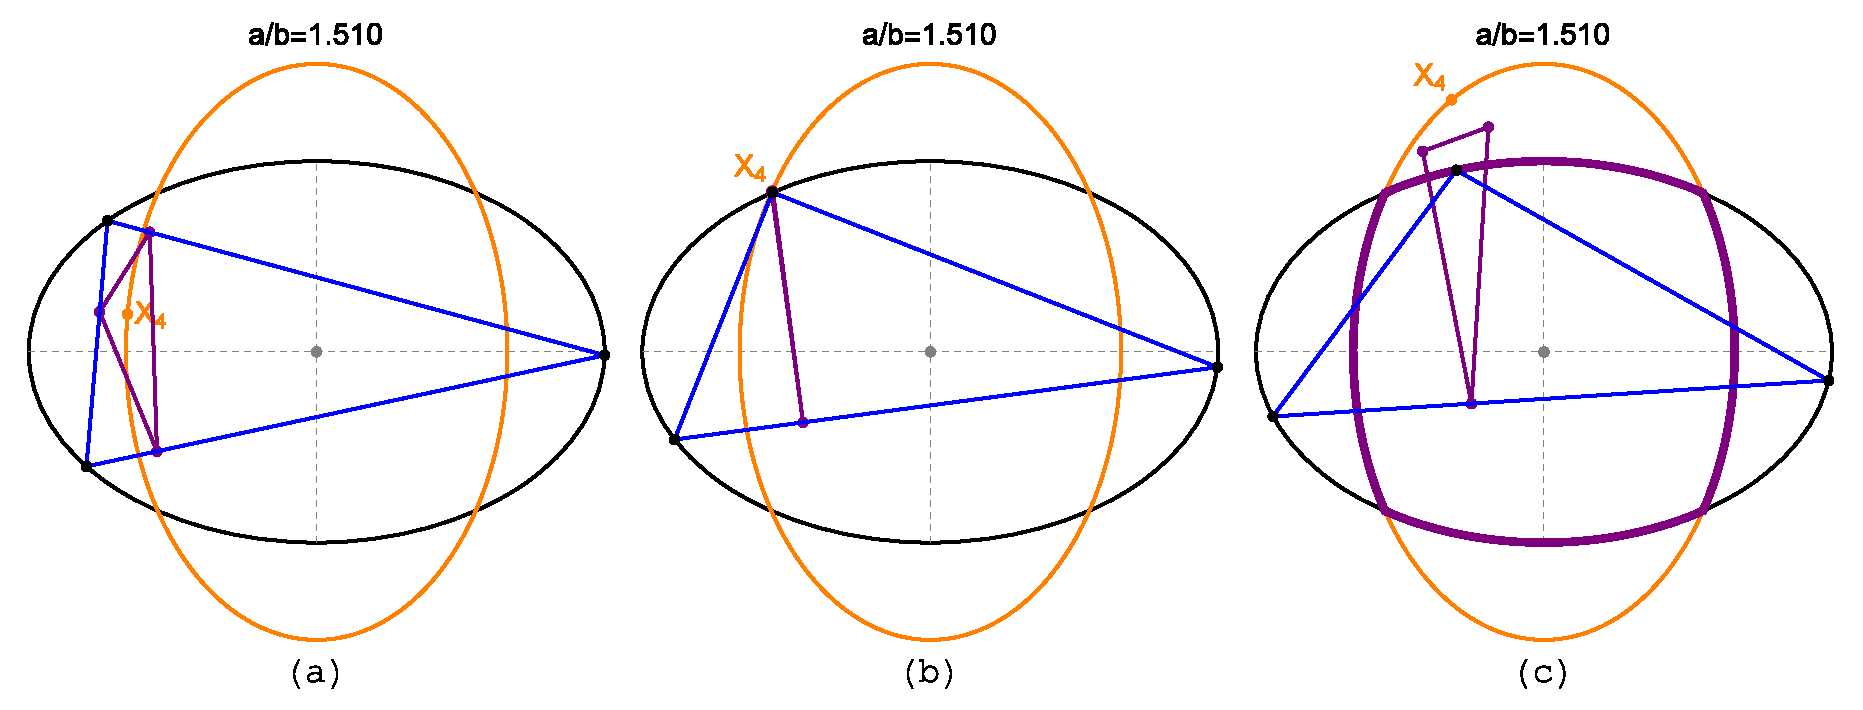
\includegraphics[trim={0 0 0 20},clip,width=\textwidth]{pics_04_120_ort_loci_kink.eps}
    \caption{From left to right: the orthic triangle (purple) of billiard 3-periodics (blue) is shown at 3 different positions. The locus of $X_4$ (orange ellipse) intersects the billiard, i.e., $a/b>\alpha_4$. When a 3-periodic is acute (left), the orthic incenter coincides with $X_4$. When it is a right triangle (middle), $X_4$ is on the elliptic billiard and the orthic is a degenerate segment. When it is obtuse (right), the orthic incenter remains ``pinned'' to the obtuse vertex. The end result is that the locus of the orthic incenter is a quadrilateral with four elliptic arcs (thick purple, right) with four corners.  \href{https://youtu.be/3qJnwpFkUFQ}{Video}, \href{https://bit.ly/33TVjit}{Live}}
    \label{fig:04-orthic_incenter_locus}
\end{figure}

\begin{proposition}
If $a/b>\alpha_4$, the locus of the incenter of the orthic triangle of billiard 3-periodics is a ``quadrilateral'' of four elliptic arcs.
\end{proposition}

To see this, let $T$ be a triangle, $T_h$ its Orthic\footnote{Its vertices are the feet of the altitudes.}, and $I_h$ be the latter's Incenter. It is well-known that if $T$ is acute $I_h$ coincides with $T$'s Orthocenter $X_4$. However, for obtuse $T$:

\begin{lemma}
$T_h$ has two vertices outside of $T$, and $I_h$ is ``pinned'' to the obtuse vertex
\label{lem:pinned}
\end{lemma}

This is a known result  \cite[Chapter 1]{coxeter67}, which we revisit in Appendix~\ref{app:orthic-incenter}. This curious phenomenon is illustrated in Figure~\ref{fig:orthic-incenter}. 

%%% BEGIN EXERCISES
\section{Exercises}

\begin{exercise}
Calculate the elliptic billiard aspect ratio $a/b$ such that top and bottom vertices of the elliptic locus of $X_3$ coincide each with the billiard top and bottom vertices. Repeat for the locus of $X_5$.
\end{exercise}

\begin{exercise}
Calculate the elliptic billiard aspect ration $a/b$ such that the locus of $X_4$ is identical to a $90^\circ$ rotated copy of billiard.
\end{exercise}

\begin{exercise}
Over billiard 3-periodics, the envelope of the Euler line is an astroidal-like curve with four cusps, see it \href{https://bit.ly/3yiCvrn}{Live}. Derive its equation. Also, find the elliptic billiard aspect ratio $a/b$ such that the top and bottom cusps of said curve coincide each with top and bottom vertices of the elliptic billiard.
\end{exercise}

\section{Blaschke Products}
\label{sec:04-blaschke}
Here we consider 3-periodics inscribed in a unit circle and circumscribing a non-concentric ellipse. We will work in the complex plane and apply Blaschke Products described in \cite{daepp-2019}, whereby Poncelet 3-periodic vertices become symmetric with respect to the information of the circle-ellipse pair. These were first used to analyze loci of Poncelet triangle centers in \cite{helman2021-power-loci}.

\begin{figure}
    \centering
    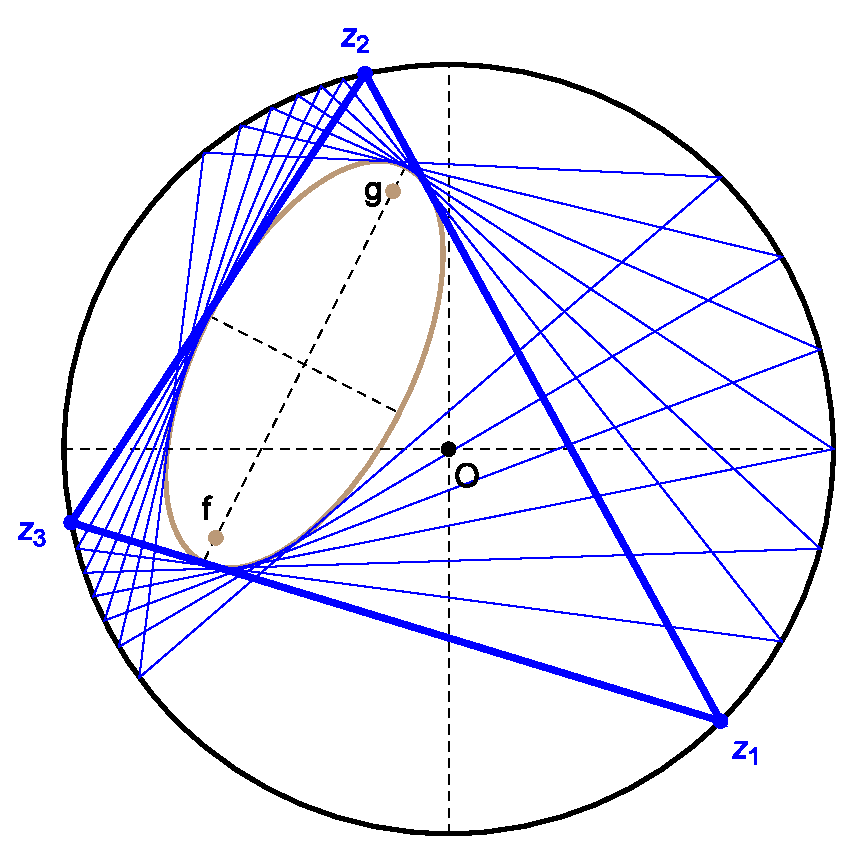
\includegraphics[width=.7\textwidth]{pics_04_050_blaschke_circum.eps}
    \caption{Blaschke complex parametrization of Poncelet 3-periodics (blue). Vertices are $z_1,z_2,z_3$. The foci of the caustic are $f,g$. }
    \label{fig:blaschke}
\end{figure}

%As a first step, identify points in $\R^2$ with points in the complex plane $\Cp$. Let $\D$ denote the open unit disk $\{z\in\Cp : |z|<1\}$ and $\T$ denote the unit circle $\{z\in\Cp : |z|=1\}$. By translation and scaling, we may assume the outer circle of the pair to be the unit circle $\T$. Let $\{f,g\}$ be the two foci of the inner ellipse.



Let  $\mathbb{T } = \{ z\in \mathbb{C}: |z| = 1\} $ the unit circle and $\mathbb{D} = \{ z\in\mathbb{C} : |z| < 1\} $ the open unit disk
bounded by $\mathbb{T }.$

Referring to \cref{fig:blaschke}, let $z_1,z_2,z_3\in\Cp$ denote the vertices of Poncelet 3-periodics in a generic $N=3$ family with fixed (unit) circumcircle denoted $\T=\{z\in\Cp : |z|=1\}$. Let $f,g$ be the foci of the caustic. Using Viète's formula, we obtain the following parametrization of the elementary symmetric polynomials on $z_1,z_2,z_3$ \cite{daepp-2019}:

\begin{definition}[Blaschke's Parametrization]
\begin{align*}
    \sigma_1:=z_1+z_2+z_3=& f+g+\l\ol f \ol g \\
    \sigma_2:=z_1 z_2+z_2 z_3+z_3 z_1=& f g+\l(\ol f+\ol g) \\
    \sigma_3:=z_1 z_2 z_3=& \l
\end{align*}
where $\l\in\T$ is the varying parameter.
\label{def:bla}
\end{definition}

\noindent Note that the concentric case occurs when $g=-f$.

For each $\l\in\T$, the three solutions of $B(z)=\l$ are the vertices of a 3-periodic orbit of the Poncelet family of triangles in the complex plane, \cite[Chapter 4]{daepp-2019}. Furthermore, as $\l$ varies in $\T$, the whole family of triangles is covered. Clearing the denominator in this equation and passing everything to the left-hand side, we get

\[
z^3-(f+g+\l\ol{f} \ol{g})z^2+(f g+\l(\ol f+\ol g))z-\l=0
\]

\begin{lemma}
If $u,v,w\in\mathbb{C}$ and $\lambda$ is a parameter that varies over the unit circle $\T\subset\mathbb{C}$, then the curve parametrized by
\[ F(\lambda)=u \lambda+ \frac{v}{\lambda}+w \]
is an ellipse centered at $w$, with semiaxis $|u|+|v|$ and $\big||u|-|v|\big|$, rotated with respect to the horizontal axis of $\mathbb{C}$ by an angle of $(\arg u+\arg v)/2$.
\label{lem:ell-param}
\end{lemma}

\begin{proof}
If either $u=0$ or $v=0$, the curve $h(\T)$ is clearly the translation of a multiple of the unit circle $\T$, and the result follows. Thus, we may assume $u\neq 0$ and $v\neq 0$.

Choose $k\in\mathbb{C}$ such that $k^2=u/v$. Write $k$ in polar form, as $k=r \mu$, where $r>0$ ($r\in\R$) and $|\mu|=1$. We define the following complex-valued functions:
\[R(z):=\mu z,~ S(z):=r z+(1/r) \ol{z},~ H(z):=k v z,~ T(z):=z+w\]

One can straight-forwardly check that $F=T\circ H\circ S\circ R$.

Since $|\mu|=1$, $R$ is a rotation of the plane, thus $R$ sends the unit circle $\T$ to itself. Since $r\in\R$, $r>0$, if we identify $\mathbb{C}$ with $\R^2$, $S$ can be seen as a linear transformation that sends $(x,y)\mapsto\left(\left(r+1/r\right)x,\left(r-1/r\right)y\right)$. Thus, $S$ sends $\T$ to an axis-aligned, origin-centered ellipse $\E_1$ with semiaxis $r+1/r$ and $|r-1/r|$. $H$ is the composition of a rotation and a homothety. $H$ sends the ellipse $\E_1$ to an origin-centered ellipse $\E_2$ rotated by an angle of $\arg(k v)=\arg(k)+\arg(v)=(\arg(u)-\arg(v))/2+\arg(v)=(\arg(u)+\arg(v))/2$. The semiaxis of $\E_2$ have length
\begin{align*}
|k v|&(r+1/r)=r|v|(r+1/r)=|r^2 v|+|v|=|k^2 v|+|v|=|u|+|v|\text{, and}\\
|k v|&|r-1/r|=r|v||r-1/r|=\big||r^2 v|-|v|\big|=\big||k^2 v|-|v|\big|=\big||u|-|v|\big|
\end{align*}

Finally, $T$ is a translation, thus $T$ sends $\E_2$ to an ellipse $\E_3$ centered at $w$, rotated by an angle $(\arg(u)+\arg(v))/2$ from the axis, with semiaxis lengths $|u|+|v|$ and $\big||u|-|v|\big|$, as desired.
\end{proof}

Consider the Moebius map $M_{z_0}=(z_0-z)/(1-\overline{z_0} z)$ and the Blaschke product of degree 3 given by   $B=M_{z_0} M_{z_1} M_{z_2}$.
\begin{theorem}
Let $B$ be a Blaschke product of degree 3 with
zeros $0, f, g.$ For $\lambda \in \mathbb{T}$, let $z_1, z_2, z_3 $ denote the three distinct solutions to $ B(z) = \lambda$. Then the
lines joining $z_j$ and $z_k$, $(j \ne k)$ are tangent to the ellipse given by
\[|w - f| + |w - g| = |1 -   \overline{f}   g |.\]
\end{theorem}
\begin{proof}
%\textcolor{red}{checar pagina}
See \cite[Theorem 2.9, page 37]{daepp-2019}.
\end{proof}

\begin{theorem}
 Given two points $f,g\in\mathbb{D}$. Then there exists a unique conic $\mathcal{E}$ with the foci
$f,g$   which is 3-Poncelet caustic with respect to $\mathbb{T}$. Moreover, $\mathcal{E}$ is an ellipse. That ellipse is
the Blaschke ellipse with the major axis of length $|1-\overline{f}g|.$
\end{theorem}

\begin{proof}
%\textcolor{red}{checar pagina}
See \cite[Corollary 4.4, page 44]{daepp-2019} and \cite{drag-milena2021}.
\end{proof}

\begin{figure}
    \centering
    \includegraphics[width=\textwidth]{pics_04_110_conv_inc_pedal.eps}
    \caption{Elliptic locus of incenter $X_1$ (green) and that of $Y_1(t)$ (pink), the convex combination of $X_1(t)$ and an intouchpoint, given by a parameter $\rho\in[0,1]$. At $\rho=1$ (top-left), $Y_1(t)$ is the recognizable two-lobe locus of the intouchpoints. Each time a 3-periodic vertex goes around the outer ellipse, $Y_1(t)$ winds once over its locus. At $\rho=0.8$ (top-right) the lobes approach each other but still lie in different half planes. At $\rho=\rho^*=1-(b/a)^2$, the lobes touch at the common center (bottom-left). If $\rho\in(0,\rho^*)$, the two lobes self-intersect twice. As $\rho{\rightarrow}0$, the two lobes become nearly coincidental (bottom-right). At $\rho=0$, the $Y_1$ locus converges to the elliptic locus of the incenter (green). This shows that that for every turn of $P_1(t)$ around the outer ellipse, $X_1$ winds thrice over its locus. \href{https://youtu.be/3Gr3Nh5-jHs}{Video 1}, \href{https://youtu.be/HZFjkWD_CnE}{Video 2}}
    \label{fig:inc-wind3}
\end{figure}
 




\section{Loci of Incenters}
\label{sec:04-proof_theorem}



In this section will give a proof of \cref{thm:03_incenter_excenter}.

\begin{proposition}\label{prop:X1c}
Over Poncelet 3-periodics in the pair with an outer circle and an ellipse in generic position, the locus $X_1$ given by:
\begin{align*}
  X_1:&\;z^4 - 2(( \bar{f} + \bar{g}) \lambda +  f g) z^2 + 8   \lambda z\\
  &+ (\bar{f} - \bar{g})^2 \lambda^2 +2 (  |f|^2 g +   f |g|^2 - 2 f - 2 g) \lambda + f^2 g^2=0\\
  \;&:\;  z^4 - 2\beta  z^2+ 8\lambda z+  (\beta^2-4\alpha\lambda) =0
\end{align*}
\end{proposition}

\begin{proof} The incenter of a triangle with vertices $\{z_1,z_2,z_3\}$ is given by:
\begin{align*}
    X_1&=\frac{\sqrt{a}\;z_1+\sqrt{b}\;z_2+\sqrt{c}\;z_3}{\sqrt{a}+\sqrt{b}+\sqrt{c}}\\
    a&=|z_2-z_3|^2, \; b=|z_1-z_3|^2, \;\; c=|z_2-z_1|^2
\end{align*}
Using that $z_i\in \T$ it follows that
\[a=2-(\frac{z_3}{z_2}+\frac{z_3}{z_2}),\;\; b=2-(\frac{z_1}{z_3}+\frac{z_3}{z_1}),\;\;c=2-(\frac{z_1}{z_2}+\frac{z_2}{z_1})\]
Eliminating the square roots in  the equation $X_1-z=0$ and using the relations  $\sigma_i$ (i=1,2,3) given in Blaschke's parametrization the result follows.
\end{proof}

\begin{proposition}
\label{prop:X1g}
Over Poncelet 3-periodics in a generic nested ellipse pair, the locus of $X_1$ is given by the following sextic polynomial in $z,\lambda$:
{\small
\begin{align*}
X_1&: \;{\lambda}^{2} \left( p^2-q^2 \right) {
z}^{4}+4\,\lambda\, \left( \alpha\,\lambda\,p q^2  - q\,{
\lambda}^{2}p^{2}-\beta\,p^2\,q+p\,q^{2} \right) {z}^{3}\\
&+  ( 4\,\alpha\,{
\lambda}^{3}p^{3} q-4\,{\alpha}^{2}{\lambda}^{2}p^{2}q^2 +2\,\alpha\,\beta\,\lambda\,p^{3}
\,q-2\,\alpha\,\beta\,\lambda\,pq^{3} -2\,\beta\,{\lambda}^{2
}p^{4}+6\,\beta\,{\lambda}^{2}p^{2}q^2\\
&-6\,\alpha\,
\lambda\,p^2\,q^{2}+2\,\alpha\,\lambda\,q^{3} q+4\,{
\beta}^{2}p^2\,q^{2}  
  +6\,{\lambda}^{2}p^{3} \,q
 -6\,{
\lambda}^{2} p q^{3}  -4\,\beta\,p\,q^{3}  ) {z}^{
2}\\
&+ ( 4 q (\alpha^2\beta p^2 q^2 + 2\alpha^2 p^2  p q - \alpha^2 p q^3 + \beta^2 p^4 - 2\beta^2 p^2 q^2+ 4\beta p q^3 - p^2 q^2 - 2 q^4)\lambda \\
&- 4\alpha  p q^2 (\beta^2 p^2 - q^2) - 4 p^3 (\beta p  q - 2 p^2 - q^2)\lambda^3 - 16\alpha\lambda^2 p^4   q ) z\\
   & -\lambda^2 (4 \alpha \lambda - \beta^2) p^6 + 4 p^5 q \lambda^4 + 2 \lambda (4 \alpha^2 \lambda - \alpha \beta^2 - 3 \beta \lambda) p^5 q   - \lambda^2 (8 \alpha \lambda - 3 \beta^2) p^4 q^2 \\
   &+ (\alpha^2 \beta^2 -4 \alpha^3 \lambda  + 4 \alpha \beta \lambda + 5 \lambda^2) p^4 q^2 + 2 \lambda (2 \alpha^2 \lambda - \alpha \beta^2 + \beta \lambda) p^3 q^3 \\
   &+ (2 \alpha^2 \beta - 2 \alpha \lambda - 4 \beta^2) p^3 q^3 - (\alpha^2 \beta^2 + 4 \alpha \beta \lambda - 4 \beta^3 + 5 \lambda^2) p^2 q^4 + ( 8 \beta-3 \alpha^2 ) p^2 q^4 \\
   &+ (2 \alpha^2 \beta + 6 \alpha \lambda - 8 \beta^2) p q^5 - 4 q^5 p + ( 4 \beta-\alpha^2 ) q^6=0
\end{align*}
}
\end{proposition}

\begin{proof} Let $p,q\in \mathbb{R}$. Consider the affine transformation
$T(z)=pz+q\ol z$ and set $w_i=T(z_i)$. The proof is similar to that given in \cref{prop:X1c}.  
\end{proof}

\begin{proposition} In the confocal pair the locus $X_1$ is defined by:
\[2\,ab{\lambda}^{2}{z}^{2}+2\,\lambda\, \left( {a}^{3}{\lambda}^{2}-{b}
^{3}{\lambda}^{2}-{a}^{3}-{b}^{3} \right) z+{c}^{2} \left( {c}^{2}{
\lambda}^{4}-2\,ab{\lambda}^{2}-{c}^{2} \right)=0 \]
\label{prop:X1q2} 
\end{proposition}

\begin{proof}
We have that
\[f={\frac {1}{c}\sqrt {-{a}^{2}-{b}^{2}+2\,\delta}}, \;\; g= -{\frac {1}{c}\sqrt {-{a}^{2}-{b}^{2}+2\,\delta}}\]
\end{proof}

\begin{corollary}
The locus $X_1$ is the ellipse with semiaxes given by $a_1=(a^2-\delta)/b$ and $b_1=(\delta-b^2)/a.$

%\[z= {\frac { \left( a-b \right)  \left(\delta -{a}^{2}-ab-{b}^{2}
 %\right) \lambda}{2\,ab}}-{\frac { \left( a+b %\right)  \left(  \delta-{a}^{2}
%+ab-{b}^{2} \right) }{2\,ab\lambda}}\]
 
\end{corollary}

\begin{proof}
The quartic polynomial is factorizable as $p_1p_2$, where
\begin{align*}
    p_1&=z-\left({\frac { \left( a-b \right)  \left( -{a}^{2}-a b-{b}^{2}+\delta
 \right) \lambda}{2\,a b}}-{\frac { \left( a+b \right)  \left( -{a}^{2}
+a b-{b}^{2}+\delta \right) }{2\,a b\lambda}}\right)
\\
    p_2&=2 a b \lambda^2 z^3 - ((a - b) (a^2 + 3 a b + b^2 + \delta) \lambda^3 - (a + b) (a^2 - 3 a b + b^2 + \delta) \lambda) z^2\\
    &+ 6 a b  (a^2 - b^2) \lambda^2 z + (a + b)^3 (a^2 - a b + b^2 + \delta) \lambda^3 - (a - b)^3 (a^2 + a b + b^2 + \delta) \lambda
\end{align*}
Follows directly from  \cref{lem:ell-param} and  \cref{prop:X1q2}.
\end{proof}

\cite{schwartz2016-com}

\begin{conjecture}
Over 3-periodics interscribed between two ellipses in general position, the locus of a triangle center $X_k$ is an ellipse if and only if $X_k$ is a fixed linear combination of $X_3$ and $X_4$.
\end{conjecture}

\begin{conjecture}
The locus of the incenter is an ellipse if and only if the Poncelet ellipse pair is confocal.
\end{conjecture}

\section{Analyzing Loci of Triangle Centers}
\label{sec:04-loci}
\begin{itemize}
    \item Triangle centers
    \item Are Loci Algebraic (method of resultants, why so many)
    \item Are Loci Elliptic (Blaschke's parametrization \cite{daepp-2019})
    \item Monotonicity and Turning Number (ballet + paper 25)
    \item Table of results
    \item A list of the elliptic loci of centers in the $X_{1}$ to $X_{200}$ range can be found \href{https://dan-reznik.github.io/why-so-many-ellipses/}{here}.
\end{itemize}

\subsection{Generic Nested Ellipses}
 
 In this Section we prove the locus of a given fixed linear combination of $X_2$ and $X_3$ is an ellipse. We will continue to use Blaschke product techniques since a generic non-concentric pair can always be seen as the affine image of a pair with circumcircle.

Consider the generic pair of nested ellipses $\E=(O,a,b)$ and $\E_c=(O_c,a_c,b_c.\theta)$ in Figure~\ref{fig:n3-general-pos}. Let s$\theta$, c$\theta$ denote the sine and cosine of $\theta$, respectively. Define $c_c^2=a_c^2-b_c^2$. The Cayley condition for the pair to admit a 3-periodic family is given by:

{\small
\begin{align}
&{b}^{4}x_c^{4}+2\,{a}^{2}{b}^{2}x_c^{2}y_c^{2}+
 \left(  2 c_c^2  \left( -{b}^{2}({a}^{2}+{b}^{2} )\right)  \text{c}\theta^2  - 2\left(  \,b ^{2}- \,b_c
^{2} \right) {b}^{2}{a}^{2}-2\,{b}^{4}b_c^{2} \right)x_c
^{2} \label{eqn:cayley}\\
&-8\,{a}^{2}{b}^{2}x_c\,{  y_c}\,c_c^2 
\text{s}\theta\text{c}\theta  +{a}^{4}y_c^{4} + \left(  2 c_c^2 a^2 \left(
{a}^{2}+{b}^{2}  \right)\text{c}\theta^2  
 -2 \left(  \,b_c^{2}+{b}^{2} \right) {a}^{4}+2
\,{a}^{2}{b}^{2}b_c^{2} \right) y_c^{2} \nonumber\\
&+ c_c^4  c^4  \left( \text{c}\theta^4-2\, c_c^2 c^2
  \left( {a}^{2} a_c^{2}-{b}^{2}{a}^{2}+
b_c^{2}{b}^{2} \right) \text{c}\theta^2 \right. \nonumber\\
 &+ \left( a a_c+a b-b b_c \right)  \left( a a_c
-a b -b b_c \right)  \left( a a_c+a b+b b_c \right)  \left( a
a_c-a b+b b_c \right) = 0\nonumber
\end{align}
}


 




Recall that over Poncelet N-periodics interscribed in a generic pair of conics, the locus of vertex and area centroids is an ellipse \cite{sergei2016-com} as is that of the circumcenter-of-mass \cite{sergei2014-circumcenter-of-mass}, a generalization of $X_3$ for $N>3$. Referring to Figure~\ref{fig:nonconcentric-xns}:

\begin{theorem}
Over the family of 3-periodics interscribed in an ellipse pair in general position (non-concentric, non-axis-aligned),
if $\X\ab$ is a fixed linear combination of $X_2$ and $X_3$, i.e., $\X\ab=\alpha X_2+\beta X_3$ for some fixed $\alpha,\beta\in\mathbb{C}$, then its locus is an ellipse. 
\label{thm:ellipse-locus}
\end{theorem}

\begin{proof}
Consider a general $N=3$ Poncelet pair of ellipses that forms a 1-parameter family of triangles. Without loss of generality, by translation and rotation, we may assume the outer ellipse is centered at the origin and axis-aligned with the plane $\R^2$, which we will also identify with the complex plane $\mathbb{C}$. Let $a,b$ be the semi-axis of the outer ellipse, and $a_c,b_c$ the semi-axis of the inner ellipse, as usual. 

Referring to Figure~\ref{fig:affine}, consider the linear transformation that takes $(x,y)\mapsto(x/a,y/b)$. This transformation takes the outer ellipse to the unit circle $\T$ and the inner ellipse to another ellipse. Thus, it transforms the general Poncelet $N=3$ system into a pair where the outer ellipse is the circumcircle, which we can parametrize using Blaschke products \cite{daepp-2019}. In fact, to get back to the original system, we must apply the inverse transformation that takes $(x,y)\mapsto(a x,b y)$. As a linear transformation from $\mathbb{C}$ to $\mathbb{C}$, we can write it as $L(z):=p z+q \ol{z}$, where $p:=(a+b)/2, q:=(a-b)/2$.

\begin{figure}
    \centering
    \includegraphics[width=\textwidth]{pics_04_030_affine_circumcircle.eps}
    \caption{Affine transformation that sends a generic ellipse pair and its 3-periodic family (left) to a new pair with circumcircle (right). We parametrize the 3-periodic orbit with vertices $z_i$ in the circumcircle pair using the foci of the latter's caustic $f$ and $g$, and then apply the inverse affine transformation to get a parametrization of the vertices $P_i$ of the original Poncelet pair. \href{https://youtu.be/6xSFBLWIkTM}{Video}}
    \label{fig:affine}
\end{figure}


Let $z_1,z_2,z_3\in\T\subset\mathbb{C}$ be the three vertices of the circumcircle family, parametrized as in Definition~\ref{def:bla}, and let $v_1:=L(z_1),v_2:=L(z_2),v_3:=L(z_3)$ be the three vertices of the original general family. The barycenter $X_2$ of the original family is given by $(v_1+v_2+v_3)/3$, and the circumcenter $X_3$ is given by \cite{stackexchange-x3a}:

\[
    X_3=\left|
        \begin{array}{ccc}
          v_1 & |v_1|^2 & 1 \\
          v_2 & |v_2|^2 & 1 \\
          v_3 & |v_3|^2 & 1
        \end{array}
      \right| \Bigg/
     \left|
        \begin{array}{ccc}
          v_1 & \overline{v_1} & 1 \\
          v_2 & \overline{v_2} & 1 \\
          v_3 & \overline{v_3} & 1
        \end{array}
      \right|
\]

Since $\ol{z_1}=1/z_1,\ol{z_2}=1/z_2,\ol{z_3}=1/z_3$, we can write $v_1,v_2,v_3$ as rational functions of $z_1,z_2,z_3$, respectively. Thus, both $X_2$ and $X_3$ are symmetric rational functions on $z_1,z_2,z_3$. Defining $\X\ab=\alpha X_2+\beta X_3$, we have consequently that $\X\ab$ is also a symmetric rational function on $z_1,z_2,z_3$. Hence, we can reduce its numerator and denominator to functions on the elementary symmetric polynomials on $z_1,z_2,z_3$. This is exactly what we need in order to use the parametrization by Blaschke products.

In fact, we explicitly compute:
\[  \X\ab= \frac{p^2 q \left(\sigma_2 (\alpha +3 \beta )+3 \beta  \sigma_3^2\right)+\alpha  p^3 \sigma_1 \sigma_3-p q^2 (3 \beta +\sigma_1 \sigma_3 (\alpha +3 \beta ))-\alpha  q^3 \sigma_2}{3 \sigma_3 (p-q) (p+q)}\]
where $\sigma_1,\sigma_2,\sigma_3$ are the elementary symmetric polynomials on $z_1,z_2,z_3$.

Let $f,g\in\mathbb{C}$ be the foci of the inner ellipse in the circumcircle system. Using Definition~\ref{def:bla}, with the parameter $\l$ varying on the unit circle $\T$, we get:

\begin{equation}
\X\ab= u \l+v\frac{1}{\l}+w
\label{eqn:xi-param}
\end{equation}

\noindent where:

\begin{align*}
    u:=&\frac{p \left(\ol{f} \ol{g} \left(\alpha  p^2-q^2 (\alpha +3 \beta )\right)+3 \beta  p q\right)}{3 (p-q) (p+q)}\\
    v:=&\frac{\beta  p q (q-f g p)}{(q-p) (p+q)}+\frac{1}{3} \alpha  f g q\\
    w:=&\frac{q \left(\ol{f}+\ol{g}\right) \left(p^2 (\alpha +3 \beta )-\alpha  q^2\right)+p (f+g) \left(\alpha  p^2-q^2 (\alpha +3 \beta )\right)}{3 (p-q) (p+q)}
\end{align*}

By   \cref{lem:ell-param}, this is the parametrization of an ellipse centered at $w$, as desired. As in  \cref{lem:ell-param}, it is also possible to explicitly calculate its axis and rotation angle, but these expressions become very long.
\end{proof}

\begin{corollary}
Over the family of 3-periodics interscribed in an ellipse pair in general position (non-concentric, non-axis-aligned),
if $\X_\gamma$ is a real affine combination of $X_2$ and $X_3$, i.e., $\X_\gamma=(1-\gamma) X_2+\gamma X_3$ for some fixed $\gamma\in\R$, then its locus is an ellipse. Moreover, as we vary $\gamma$, the centers of the loci of the $\X_\gamma$ are collinear.
\end{corollary}

\begin{proof}
Apply   \cref{thm:ellipse-locus} with $\alpha=1-\gamma, \beta=\gamma$ to get the elliptical loci. As in the end of the proof of  \cref{thm:ellipse-locus}, the center of the locus of $\X_\gamma$ can be computed explicitly as 
\begin{gather*}
    w=w_0+w_1 \gamma \text{, where}\\
    w_0=\frac{1}{3} \left(q \left(\ol{f}+\ol{g}\right)+p (f+g)\right)\\
    w_1=\frac{q \left(2 p^2+q^2\right) \left(\ol{f}+\ol{g}\right)-p (f+g) \left(p^2+2 q^2\right)}{3 (p-q) (p+q)}
\end{gather*}
As $\gamma\in\R$ varies, it is clear the center $w$ sweeps a line.
\end{proof}

We proved that all of the following triangle centers have elliptic loci in the general N=3 Poncelet system, including the barycenter, circumcenter, orthocenter, nine-point center, and de Longchamps point (reflection of the orthocenter  about the circumcenter of a triangle):

\begin{observation}
Amongst the 40k+ centers listed on \cite{etc}, about 4.9k triangle centers lie on the Euler line \cite{etc-central-lines}. Out of these, only 226 are fixed affine combinations of $X_2$ and $X_3$. For $k<1000$, these amount to $X_k,k=${\small 2, 3, 4, 5, 20, 140, 376, 381, 382, 546, 547, 548, 549, 550, 631, 
632}.
\label{obs:affine-euler-line}
\end{observation}

\begin{figure}
     \centering
     \includegraphics[width=.8\textwidth]{pics_04_020_n3_nonconcentric_conics.eps}
     \caption{A 3-periodic is shown interscribed between two nonconcentric, non-aligned ellipses (black). The loci of $X_k$, $k=2,3,4,5,20$ (and many others) remain ellipses. Those of $X_2$ and $X_4$ remain axis-aligned with the outer one. Furthermore the centers of all said elliptic loci are collinear (magenta line). \href{https://youtu.be/p1medAei_As}{Video}}
     \label{fig:nonconcentric-xns}
 \end{figure}
 
%\begin{corollary}
%The elliptic loci of $X_2$, $X_3$ and $X_4$ are given by:
%\[ \textcolor{red}{mark} \]
%\textcolor{red}{these will be hard to get explicitly}
%\end{corollary}
 
\begin{observation}\label{obs:X2X4}
The elliptic loci of $X_2$ and $X_4$ are axis-aligned with the outer ellipse.
\end{observation} 

We conclude this section with phenomenon specific to the case where $\E_c$ is a circle,  ~\cref{fig:circular-caustic}:

\begin{observation}
 Over the family of 3-periodics inscribed in an ellipse and circumscribing a non-concentric circle centered on $O_c=X_1$, the locus of $X_3$ and $X_5$ are ellipses whose major axes pass through $X_1$.
 \end{observation}
 
\begin{figure}
    \centering
    \includegraphics[width=.7\textwidth]{pics_04_040_n3_nonconcentric_circular_caustic.eps}
    \caption{A 3-periodic (blue) is shown inscribed in an outer ellipse and an inner non-concentric circle centered on $O_c$. The loci of both circumcenter (solid red) and Euler center (solid green) are ellipses whose major axes pass through $O_c$. \href{https://youtu.be/w7sZ5O8k4xU}{Video}}
    \label{fig:circular-caustic}
\end{figure}



Referring to Figure~\ref{fig:nonconcentric-circumcircle-circular-loci-right-tris}:

\begin{proposition}
If a triangle center $\X\ab=\alpha X_2+ \beta X_3$ is a fixed linear combination of $X_2$ and $X_3$ for some $\alpha,\beta\in\mathbb{C}$, its locus over 3-periodics in the non-concentric pair with a circumcircle is a circle centered on $\mathcal{O}_\alpha$ and of radius $\mathcal{R}_\alpha$ given by:

\[ \mathcal{O}_\alpha = \frac{\alpha(f+g)}{3},\;\;\; \mathcal{R}_\alpha =\frac{|\alpha f g|}{3}\]
\label{prop:LinComb-concentric}
\end{proposition}

\begin{observation}
Notice that the center and radius of the locus do not depend on $\beta$ since the circumcenter $X_3$ is stationary at the origin of this system.
\end{observation}

\begin{proof}
Since, $z_1,z_2,z_3$ are the 3 vertices of the Poncelet triangle inscribed in the unit circle, its barycenter and circumcenter are given by $X_2=(z_1+z_2+z_3)/3$ and $X_3=0$, respectively. We define $\X\ab:=\alpha X_2+ \beta X_3=\alpha (z_1+z_2+z_3)/3$. Using Definition~\ref{def:bla}, we get $\X\ab=\alpha(f+g+\l \ol{f}\ol{g})/3=\alpha(f+g)/3+\l(\alpha \ol{f}\ol{g})/3$, where the parameter $\l$ varies on the unit circle $\T$. Thus, the locus of $\X_{\gamma}$ over the Poncelet family of triangles is a circle with center $\mathcal{O}_{\alpha}:=\alpha(f+g)/3$ and radius $\mathcal{R}_{\alpha}:=|\alpha \ol{f}\ol{g}|/3=|\alpha f g|/3$.
\end{proof}

Using $\alpha=1-\gamma, \beta=\gamma$ for a fixed $\gamma\in\R$ in   \cref{prop:LinComb-concentric}, we get:

\begin{corollary}
 If a triangle center $\X_\gamma=(1-\gamma) X_2+ \gamma X_3$ is a real affine combination of $X_2$ and $X_3$ for some $\gamma\in\R$, its locus over 3-periodics in the non-concentric pair with a circumcircle is a circle. Moreover, as we vary $\gamma$, the centers of these loci are collinear with the fixed circumcenter.
 \label{cor:gamma-with-circumcircle}
\end{corollary}

Many triangle centers in \cite{etc} are affine combinations of the barycenter $X_2$ and circumcenter $X_3$. See   \cref{obs:affine-euler-line} for a compilation of them.

\begin{observation}
For a generic triangle, only $X_{98}$, and $X_{99}$ are simultaneously on the Euler line and on the circumcircle. However these are not linear combinations of $X_2$ and $X_3$. Still, if a triangle center is always on the circumcircle of a generic triangle (there are many of these, see \cite[Circumcircle]{mw}), its locus over 3-periodics in the non-concentric pair with circumcircle is trivially a circle.
\end{observation}

 
\begin{corollary}
 Over the family of 3-periodics inscribed in a circle and circumscribing a non-concentric inellipse centered at $O_c$, the locus of $X_k$, $k$ in 2,4,5,20 are circles whose centers are collinear. The locus of $X_5$ is centered on $O_c$. The centers and radii of these circular loci are given by:

\begin{alignat*}{4}
    O_2&=\frac{f+g}{3},\quad& O_4&=f+g,\quad&O_5&=\frac{f+g}{2},\quad&O_{20}&=-(f+g)\\
    r_2&=\frac{|f g|}{3},\quad&r_4 &= |f g|,\quad&r_5 &= \frac{|f g|}{2},\quad& r_{20}&= |f g|
\end{alignat*}

\end{corollary}

\begin{proof}
As in  \cref{cor:gamma-with-circumcircle}, we can use  \cref{prop:LinComb-concentric} with $\gamma=0,-2,-1/2,4$ to get the center and radius for $X_2,X_4,X_5,X_{20}$, respectively. All of these centers are real multiples of $f+g$, so they are all collinear. Moreover, the center $O_5$ of the circular loci of $X_5$ is $(f+g)/2$, that is, the midpoint of the foci of the inellipse, or in other words, the center $O_c$ of the inellipse.
\end{proof}
 
Referring to  \cref{fig:nonconcentric-circumcircle-circular-loci-right-tris}:

\begin{observation}
The family of 3-periodics in the pair with circumcircle includes obtuse triangles if and only if $X_3$ is exterior to the caustic. \end{observation}

This is due to the fact that when $X_3$ is interior to the caustic, said triangle center can never be exterior to the 3-periodic. Conversely, if $X_3$ is exterior, it must also be external to some 3-periodic, rendering the latter obtuse.

\begin{figure}
    \centering
    \includegraphics[width=\textwidth]{pics_03_010_n3_circumcircle_pair.eps}
    \caption{\textbf{Left:} 3-periodic family (blue) in the pair with circumcircle where the caustic contains $X_3$, i.e., all 3-periodics are acute. The loci of $X_4$ and $X_{20}$ are interior to the circumcircle. \textbf{Right:} $X_3$ is exterior to the caustic, and 3-periodics can be either acute or obtuse. Equivalently, the locus of $X_4$ intersects the circumcircle. In both cases (left and right), the loci of $X_k$, $k$ in 2,4,5,20 are circles with collinear centers (magenta line). The locus of $X_5$ is centered on $O_c$. The center of the $X_2$ locus is at $2/3$ along $O O_c$. \href{https://youtu.be/HXgJQo2UT_8}{Video}}
    \label{fig:nonconcentric-circumcircle-circular-loci-right-tris}
\end{figure} 


Consider the parametrization of a triangular orbit $\{z_1,z_2,z_3\}$ given in \cref{def:bla}.

Let also the  affine transformation
$T(z)=pz+q\ol z$.

\textcolor{red}{figura do blaschke}

\begin{theorem}
Over the family of 3-periodics interscribed in a generic nested pair of ellipses (non-concentric, non-axis-aligned),
if $\X\ab$ is a fixed linear combination of $X_2$ and $X_3$, i.e., $\X\ab=\alpha X_2+\beta X_3$ for some fixed $\alpha,\beta\in\mathbb{C}$, then its locus is an ellipse. 
\label{thm:ellipse-locus}
\end{theorem}




\section{Loci of Rational Triangle Centers}
\label{sec:04-rational-trilinears}



Consider a Triangle Center $X$ whose Trilinears $p:q:r$ are rational on the sidelengths $s_1,s_2,s_3$, i.e., the Triangle Center Function $h$ is rational, see  
\cref{eqn:appAtrilin-cartesian}

\begin{theorem} In the family of 3-periodic orbits in a Poncelet pair of ellipses, axis parallel and common center, the locus of a rational triangle center is an algebraic curve.
\label{thm:rational-center}
\end{theorem}

Our proof is based on the following 3-steps which yield an algebraic curve $\mathcal{L}(x,y)=0$ which contains the locus. We refer to \cref{lem:1coord} and \cref{lem:2sides} appearing below. %Appendix~\ref{app:rational-support} contains  supporting expressions.

\begin{proof}

\begin{step}
Introduce the symbolic variables $u, u_1, u_2$:

\begin{equation*}
    u^2 + u_1^2 = 1,\;\;\;   u_2^2 = k_1u^2+k_2.
\end{equation*} % \smallskip

\end{step}
 
\noindent The vertices will be given by rational functions of   $u, u_1, u_2$ 
\begin{equation*} P_1 = (a\,u, b\,u_1),\;\;P_2 = (p_{2x}, p_{2y})/p_3,\;\;\;P_3 = (p_{3x}, p_{3y})/p_3 
\end{equation*}
 
\noindent Expressions for $P_1,P_2,P_3$ appear in \cref{eq:03-n3-conc-general} as do equations $g_i=0$, $i=1,2,3$, polynomial in $ s_i,u,u_1,u_2$.
 
\begin{step}Express the locus  $X$ as a  rational function on  $u,u_1, u_2, s_1, s_2, s_3$.
\end{step}

Convert $p:q:r$ to Cartesians $ X = (x,y)$ via  \cref{eqn:appAtrilin-cartesian}. From  \cref{lem:1coord}, it follows that
$\left(x,y\right)$ is rational on $u,u_1,u_2,s_1,s_2,s_3$.

\begin{equation*} x=\mathcal{Q}/\mathcal{R},\;\;\;y=\mathcal{S}/\mathcal{T}
\end{equation*}

\noindent To obtain the polynomials    $\mathcal{Q,R,S,T}$  on said variables $u,u_1,u_2,s_1,s_2,s_3$,
 one substitutes the 
$p,q,r$ by the corresponding rational functions of  $s_1, s_2, s_3$ that define a specific Triangle Center $X$. Other than that, the method proceeds identically.

\begin{step}
Computing resultants.
Our problem is now cast in terms of the polynomial equations:

\begin{equation*}
E_0= \mathcal{Q}-x\,\mathcal{R}=0,\;\;\; F_0= \mathcal{S}-y\,\mathcal{T}=0
\end{equation*}

\end{step}

%Let $g_1$, $g_2$ and $g_3$ be the polynomials in Appendix~\ref{app:alg_locus}. 
Firstly, compute the resultants, in chain fashion:  

\begin{align*}
    E_1=&\textrm{Res}(g_1,E_0,s_1)=0,\;\;\;F_1=\textrm{Res}(g_1,F_0,s_1)=0\\
	E_2=&\textrm{Res}(g_2,E_1,s_2)=0,\;\;\;F_2=\textrm{Res}(g_2,F_1,s_2)=0\\
	E_3=&\textrm{Res}(g_3,E_2,s_3)=0,\;\;\;F_3=\;\textrm{Res}(g_3,F_2,s_3)=0
\end{align*}
		 
It follows that  $E_3(x,u,u_1,u_2)=0$ and $F_3(y,u,u_1,u_2)=0$ are polynomial
equations. In other words, $s_1, s_2, s_3$ have been eliminated. 

Now  eliminate the variables $u_1$ and $u_2$ by taking the following resultants:

\begin{align*}
	E_4(x,u,u_2)=&\textrm{Res}(E_3,u_1^2+u^2-1,u_1)=0\\ 	F_4(y,u,u_2)=&\textrm{Res}(F_3,u_1^2+u^2-1,u_1)=0\\
	E_5(x,u)=&\textrm{Res}(E_4,u_2^2+\rho_1 u^2-1,u_2)=0\\
	F_5(y,u)=&\textrm{Res}(F_4,u_2^2+\rho_1 u^2-1,u_2)=0
\end{align*}

This yields two polynomial equations $E_5(x,u)=0$ and $F_5(y,u)=0$. 

Finally compute the resultant
$$ {\mathcal L} = \textrm{Res}(E_5,F_5,u)=0
$$
that eliminates $u$ and gives  the implicit algebraic equation for the locus $X$. 
\end{proof}

\begin{remark}
In practice,  after  obtaining  a resultant, a human assists the CAS by factoring out spurious branches
(when recognized), in order to get the final answer in more reduced form.   
\end{remark}

When not rational in the sidelengths, except a few cases\footnote{For instance Hofstadter points $X(359), X(360)$.}, Triangle Centers
in Kimberling's list have explicit Trilinears involving fractional powers and/or terms containing the triangle area. Those can be made implicit, i.e,
given by zero sets of polynomials involving $p,q,r, s_1, s_2, s_3$.  The chain of resultants to be computed will be increased by three, in order to eliminate the variables $p,q, r$ before (or after) $s_1, s_2, s_3$.

\subsubsection{Supporting Lemmas}
\label{sec:supporting-lemmas}

\begin{lemma}
\label{lem:1coord}
Let $P_1=({a}{u},b\sqrt{1-u^2}).$
	The coordinates of $P_2$ and $P_3$ of the 3-periodic billiard orbit are rational functions in the variables $u, u_1, u_2$, where
	$u_1=\sqrt{1-u^2}$, $u_2=\sqrt{k_1+k_2 u^2}$ 
and
%\textcolor{red}{checar valores de k1 e k2}
	$k_1= a_c^2(b^2 - b_c^2)a^2b^2,$ $ k_2= a^2b^2(a^2b_c^2 - a_c^2b^2)$.  
		
	\end{lemma}
	
	\begin{proof}
	Follows directly from the parametrization of the Poncelet orbit, see \cref{eq:03-n3-conc-general}.
 
	In fact,  $P_2=(x_2(u),y_2(u)) =( p_{2x}/A_{11}, p_{2y}/A_{11})$ and $P_3=(x_3(u),y_3(u))$ $=( p_{3x}/A_{11}, p_{3y}/A_{11})$, where $p_{2x}$, $p_{2y}$, $p_{3x}$ and $p_{3y}$ have degree $2$ in $(u,u_1,u_2)$  and $A_{11}$ algebraic of degree $2$ in $u$. 
%	Expressions for $u_1,u_2$ appear in %Appendix~\ref{app:exit-angle}.	\textcolor{red}{ver equacao a referenciar}
\end{proof}
	
\begin{lemma}
\label{lem:2sides} Let $P_1=(a u,b\sqrt{1-u^2}).$ Let $s_1$, $s_2$ and $s_3$ the sides of the triangular orbit ${P_1}{P_2}{P_3}$. Then $g_1(u,s_1)=0$, $g_2(s_2,u_2,u)=0$ and $g_3(s_3,u_2,u)=0$ for polynomial functions $g_i$.  
\end{lemma}
	
\begin{proof}
Using the parametrization of the 3-periodic Poncelet orbit it follows that $s_1^2-|P_2-P_3|^2=0$ is a rational equation in the variables $u,s_1$. Simplifying, leads to $g_1(s_1,u)=0.$

Analogously for $s_2$ and $s_3$. In this case, the equations $s_2^2-|P_1-P_3|^2=0$ and  $s_3^2-|P_1-P_2|^2=0$   have   square roots $u_2=\sqrt{k_2-k_1 u^2}$ and $u_1=\sqrt{1-u^2}$ and  are rational in the variables $s_2,u_2,u_1,u$ and $s_3,u_2,u_1,u$ respectively. It follows that the degrees of $g_1$, $g_2$, and $g_3$ are $10$.  Simplifying, leads to $g_2(s_2,u_2,u_1,u)=0 $ and $g_3(s_3,u_2,u_1,u)=0$. 
\end{proof}


 \begin{theorem}\label{thm:loci_algebraic_general}
 In the family of 3-periodic orbits in a generic Poncelet pair of conics the locus of a rational triangle center is an algebraic curve. 
 \end{theorem}

 \begin{proof}
 The analysis follow the same steps as in the case of a Poncelet pair of ellipses.  See proof of \cref{thm:rational-center}. 
\end{proof}

\section{Exercises}
\label{sec:04-exercises}
\section{Exercises}

\begin{exercise}
Show that over the poristic family, the locus of the foci of the $X_9$-centered circumconic (the circumbilliard) is a circle.
\end{exercise}

\begin{exercise}
Prove \cref{prop:04-antiorthic}. Furthermore, prove the intersection point of $X_1 X_3$ with the antiorthic axis is the Schröder point $X_{1155}$.
\end{exercise}

\begin{exercise}
Prove that over the poristic family the inconic centered on $X_1$ is axis-parallel with the circumconic centered on $X_9$ (i.e., the circumbilliard), see this \href{https://youtu.be/0VHBjdHXbJc}{Video}.
\end{exercise}


\begin{exercise}
Recall the cosine circle $\Cm$ (also known as the second Lemoine circle) is centered on a triangle's symmedian point $X_6$. Let $\E'$ be the Brocard ellipse of some triangle $T$. Let $\beta$ be the aspect ratio of $\E'$, i.e., $a'/b'$. Show that for any $T$, above (resp. below) a certain $\beta$, $\Cm$ is tangent to $\E'$ at two distinct points (resp. it is exterior to $\E'$). See it \href{https://bit.ly/2RqhUQV}{Live}.
\end{exercise}


\begin{exercise}
Show that the poristic excentral family is also the polar image of billiard excentrals wrt to a circle centered on a billiard (i.e., the caustic) focus. See it \href{https://bit.ly/33c1s9A}{Live}.
\end{exercise}

\begin{exercise}
Show that over the Brocard porism the radius $r^*$ of the cosine circle is invariant.
\end{exercise}

\begin{exercise}
Show that the first Lemoine circle (centered on $X_{182}$ is stationary over the Brocard porism. Above a certain $a'/b'$, this circle is tangent to one of the minor vertices of the caustic. See it \href{https://bit.ly/3tp0XUq}{Live}.
\end{exercise}

\begin{exercise}
Ehrmann's ``third'' Lemoine circle is studied in \cite{darij2012-ehrmann}, centered on $X_{576}$, is defined as follows: for each vertex, consider the 3 circles containing pairs of vertices and the symmedian point $X_6$. The third Lemoine circle contains the 6 intersections of said circles (2 each) with the sidelines. Prove this circle is also stationary over the Brocard porism, i.e., all three Lemoine circles are; see it \href{https://bit.ly/3tw09gA}{Live}. 
\end{exercise}


\begin{exercise}
Prove the expression and inequality for $\cot{\omega}$ in \cref{prop:04-brocard-w}.
\end{exercise}

\begin{exercise}
That the Brocard axis $X_3 X_6$ is stationary over the Brocard porism is established. Prove that the Lemoine axis, which intersects the Brocard axis at the Schoutte point $X_{187}$, is also stationary; see it \href{https://bit.ly/3nTRi75}{Live}.
\end{exercise}

\begin{exercise}
The so-called ``second'' Brocard triangle, defined in \cite[Second Brocard Triangle]{mw}, has vertices at the intersections of symmedians (cevians through $X_6$) with the Brocard circle. Show that over the Brocard porism, the family of second Brocard triangles is a new, smaller Brocard porism which shares the isodynamic points $X_{15}$ and $X_{16}$ with the original family. Prove that if this is iterated, the shrinking porisms converge to $X_{15}$. See it \href{https://bit.ly/3ttMNBg}{Live}.
\end{exercise}



\chapter[Confocal Loci]{Locus Phenomena in the Confocal Family}
\label{chap:05-confocal-loci}
When we consider Poncelet 3-periodic families, a natural (and indeed early) question was ``what are the loci of certain traingle centers''. Recall one of our early experimental finds: that over billiard 3-periodics, the locus of the incenter $X_1$ is an ellipse (as is that of the excenters), see \cref{sec:02-inc-exc-loci}. Also an early find was that the ``locus'' of the Mittenpunkt $X_9$ is a point, see \cref{sec:02-stationary}.

In this chapter we expand on this exploration of loci of triangle centers, touring a gallery of interesting locus-related phenomena, including:

\begin{itemize}
    \item The loci of some notable centers of a triangle, showing thy are ellipses;
    \item Billiard 3-periodics which can be both acute and obtuse;
    \item A triangle center with a non-elliptic (quartic) locus nearly identical to an ellipse;
    \item Two special triangle centers railed to either the billiard or the confocal caustic;
    \item A non-smooth locus with four singularities;
    \item A self-intersecting locus;
    \item A non-compact, non-elliptic locus;
    \item An elliptic locus whose aspect ratio is the golden ratio $\varphi$;
    \item A triangle center railed to the elliptic billiard whose motion with respect to 3-periodic vertices is ``non-monotonic'';
    \item The non-elliptic loci of the vertices of certain derived triangles. 
    \item The ``triple-winding'' of triangle center loci over themselves.
\end{itemize}

\section{Kimberling centers with elliptic loci}

The semi-axes $a_1,b_1$ for the elliptic locus of the incenter $X_1$ were given in \cref{thm:02-incenter-excenter}. It turns the loci of the next four centers in \cite{etc} are also ellipses. There are the barycenter $X_2$, the circumcenter $X_3$, the orthocenter $X_4$, and the center of the 9-point circle (also known as Euler's circle) $X_5$. Their semi-axes are given by:

\begin{align*}
    \left(a_2,b_2\right)=&k_2\left(a,b\right),\;\text{with}\; k_2=\frac{2\delta -a^{2}-b^{2}}{3c^2}\\
     \left(a_3,b_3\right)=&\left(\frac{a^{2}-\delta}{2a},\frac{\delta-b^{2}}{2b}\right)\\
 \left(a_4,b_4\right)=&\left(\frac{k_4}a,\frac{k_4}b\right),\;\text{with}\;k_4=\frac{  (a^{2}+b^{2})\delta-2\,a^{2}b^{2} }{c^2}\\
   \left(a_5,b_5\right)=&\left(\frac{- w'_5(a,b)+ w''_5(a,b) \delta}{ w_5(a,b)},\;\frac{ w'_5(b,a)-{w''_5(b,a) \delta}}{w_5(b,a)}\right)
\end{align*}
where $w'_5(u,v)=u^2(u^2+3v^2)$, $w''_5(u,v)=3u^2+ v^2$, and $w_5(u,v)=4u(u^2-v^2)$. Note that (i) $a_2/b_2=a/b$ and (ii) $b_4/a_4=a/b$.

As it turns out, the locus of 49 out of the first 200 centers in \cite{etc} are ellipses. These are: $X_k$, $k=$1,  2,  3,  4,  5,  7,  8,  10,  11,  12,  20,  21,  35,  36,  40,  46,  55,  56,  57,  63,  65,  72,  78,  79,  80,  84,  88,  90,  100,  104,  119,  140,  142,  144,  145,  149,  153,  162,  165,  190,  191,  200. Links to live animations as well as expressions for their semi-axes are provided in \cite{garcia2021-ellipses-web}.

%% Swans
%% the following centers lie on the $X_9$-centered circumellipse: 88, 100, 162, 190 \cite{etc}.

\begin{figure}
\centering
\includegraphics[width=.6\textwidth]{pics_05_060_locus_x12345.pdf}
\caption{Over billiard 3-periodics, the loci of incenter $X_1$, barycenter $X_2$, circumcenter $X_3$, orthocenter $X_4$, and 9-point center $X_5$ are all ellipses. The Euler line (dashed black) is shown passing through all but the first center. \href{https://youtu.be/sMcNzcYaqtg}{Video}, \href{https://bit.ly/3eVScgE}{Live}}
\label{fig:05-x12345}
\end{figure}

%%% begin X4
\section{When billiard 3-periodics are obtuse}

\begin{figure}
    \centering
    \includegraphics[width=\textwidth]{pics_05_130_ort_loci}
    \caption{Locus of the orthocenter (orange) over elliptic billiards with different aspect ratios. If $a/b$ is (i) less than (resp. (ii) equal, (iii) greater than) $\alpha_4{\simeq}1.352$, the locus of the orthocenter $X_4$ (orange) is (i) interior (resp. (ii) internally tangent, (iii) intersecting) with the elliptic billiard. In (i) and (ii) all 3-periodics are acute, whereas in (iii) some will be obtuse.}
    \label{fig:05-orthocenter-loci}
\end{figure}

It turns out the locus of $X_4$ can be used to determine if the billiard 3-period family will contain obtuse triangles. Referring to Figure~\ref{fig:05-orthocenter-loci}:

\begin{proposition}
The locus of $X_4$ is internally tangent to the elliptic billiard at its top and bottom vertices when $a/b=\alpha_4$ given by:

\[\alpha_4 = \sqrt{2\,\sqrt {2}-1}\;{\simeq}\;1.352.\]
\label{prop:05-alpha4}
\end{proposition}

\begin{proof}
The equation $b_4=b$ is equivalent to $a^4+2a^2b^2-7b^4=0.$ Therefore, as $a>b>0$, it follows that $a/b=\sqrt{2\,\sqrt {2}-1}.$
\end{proof}

\noindent Let $\alpha_4^*$ be the positive root of
${x}^{6}+{x}^{4}-4\,{x}^{3}-{x}^{2}-1=0$, i.e.,
$\alpha_4^{*}={\simeq}\;1.51$. 

\begin{proposition}
When $a/b=\alpha_4^{*}$, then $a_4=b$ and $b_4=a$, i.e., the locus of $X_4$ is identical to a rotated copy of Billiard. 
\end{proposition}

\begin{proof}
The condition $a_4=b$, or equivalently $b_4=a$, is defined by $a^6+a^4b^2-4a^3b^3-a^2b^4-b^6=0$. Graphic analysis shows that ${x}^{6}+{x}^{4}-4\,{x}^{3}-{x}^{2}-1=0$ has only one positive real root which we call $\alpha_4^*$.
\end{proof}

\begin{theorem}
If $a/b<\alpha_4$ (resp. $a/b>\alpha_4$) the 3-periodic family will not (resp. will) contain obtuse triangles.
\end{theorem}

\begin{proof}
If the 3-periodic is acute, $X_4$ is in its interior, therefore also internal to the EB. If the 3-periodic is a right triangle, $X_4$ lies on the right-angle vertex and is therefore on the EB. If the 3-periodic is obtuse, $X_4$ lies on exterior wedge between sides incident on the obtuse vertex (feet of altitudes are exterior). Since the latter is on the EB, $X_4$ is exterior to the EB.
\end{proof}

Another way to think of this is depicted in \cref{fig:05-obtuse-zones}: $a/b>\alpha_4$, opens up two ``zones'' along the top and bottom halves of the elliptic billiard. A 3-periodic will be obtuse if and only if one of its vertices is on either zone. These zones are precisely portions of the elliptic billiard which are interior to the locus of $X_4$; see \cref{fig:05-orthocenter-loci}(right). When $a/b=\alpha_4$ said zones collapse to the top and bottom vertices of the elliptic billiard; see \cref{fig:05-orthocenter-loci}(bottom left).

\begin{figure}
    \centering
    \includegraphics[width=.66\textwidth]{pics_05_150_rect_zones}
    \caption{Both acute (blue) and obtuse (dashed blue) billiard 3-periodics are shown. In this case $a/b=1.618>\alpha_4$. If a 3-periodic vertex is located in the red arcs along the top and bottom halves of the elliptic billiard, the 3-periodic will be obtuse.}
\label{fig:05-obtuse-zones}
\end{figure}

%%% end X4

%%% begin X6
\section{Quartic locus of the symmedian point \torp{$X_6$}{X(6)}}
\label{sec:symmedian}

The symmedian point $X_6$ is replete with properties, indeed it is known as the crown jewel of triangle geometry \cite[Symmedian Point]{mw}. Its construction is deceptively simple: the point where a triangle's {\em symmedians} concur; these are reflections of medians on the bisectors. Its trilinear coordinates could not be simpler: $[a:b:c]$. However, it is the first Kimberling center whose locus over billiard 3-periodics is {\em not} an ellipse. 

In fact, when $1<a/b<2$, its locus is visually indistinguishable from a true ellipse; see Figure~\ref{fig:05-locus-x6}. Fortunately, its fit error is easily detectable with numerical methods. Indeed:

\begin{proposition}
The locus of $X_6$ is a convex quartic given by:

\begin{equation*}
  \X_6(x,y)=c_1 x^4+c_2 y^4+c_3 x^2 y^2+ c_4 x^2 + c_5 y^2 = 0
\end{equation*}

\noindent where:
$$
\begin{array}{rlrl}
c_1=&b^4(5\delta^2-4(a^2-b^2)\delta -a^2 b^2)&c_2=&a^4(5\delta^2+4(a^2-b^2)\delta-a^2b^2) \\
c_3=&2a^2 b^2(a^2 b^2+3\delta^2)&c_4=&a^2 b^4(3 b^4+2(2 a^2-b^2)\delta-5\delta^2)\\
c_5=&a^4 b^2(3 a^4+2(2 b^2-a^2)\delta-5\delta^2)&\delta=&\sqrt{a^4-a^2 b^2+b^4}
\end{array}
$$
\end{proposition}

\begin{proof}
Using a CAS, obtain symbolic expressions for the coefficients of a quartic symmetric about both axes (no odd-degree terms), passing through 5 known-points. Still using a CAS, verify the symbolic parametric for the locus satisfies the quartic.
\end{proof}

 \noindent Note the above is also satisfied by a degenerate level curve $(x,y)=(0,0)$, which we ignore.

\begin{remark}
We term the ``best-fit'' ellipse $\mathcal{E}_6$ the one internally-tangent to $\X_6(x,y)=0$ at its four vertices. Its semi-axes are given by: 

{\small  
\begin{align*}
%a_6=&\frac{\left[(3\,a^2-b^2)\delta %-(a^2+b^2)b^2\right]a}{a^4+b^4+2\delta^2}\nonumber\\
a_6= \frac{\left[(3\,a^2-b^2)\delta -(a^2+b^2)b^2\right]a}{a^2b^2+3\delta^2},\;\;\;
b_6= \frac{\left[(a^2-3\,b^2)\delta + (a^2+b^2)a^2\right]b}{a^2b^2+3\delta^2}
\label{eqn:x6-ellipse}
\end{align*}
}
\end{remark}

Table~\ref{tab:quartic-coeffs} shows the above coefficients numerically for a few values of $a/b$.

\begin{table}
    \centering
$$
\begin{array}{|c|c|c|c|c|c|c|c|}
\hline
 \text{a/b} & a_6 & b_6 & c_1/c_3 & c_2/c_3 & c_4/c_3 & c_5/c_3 & A(\mathcal{E}_6)/A(\mathcal{X}_6) \\
 \hline
  1.25 & 0.433 & 0.282 & 0.211 & 1.185 & -0.040 & -0.095 & 0.9999 \\
 1.50 & 0.874 & 0.427 & 0.114 & 2.184 & -0.087 & -0.399 & 0.9998 \\
 2.00 & 1.612 & 0.549 & 0.052 & 4.850 & -0.134 & -1.461 & 0.9983 \\
 3.00 & 2.791 & 0.620 & 0.020 & 12.423 & -0.157 & -4.769 & 0.9949 \\
 \hline
\end{array}
$$
\caption{Coefficients $c_i/c_3$, $i=1,2,4,5$ for the quartic locus of $X_6$ as well as the axes $a_6,b_6$ for the best-fit ellipse, for various values of $a/b$. The last-column reports the area ratio of the internal ellipse $\mathcal{E}_6$ (with axes $a_6,b_6$) to that of the quartic locus $\mathcal{X}_6$, showing an almost exact match.}
\label{tab:quartic-coeffs}
\end{table}


\begin{figure}
    \centering
    \includegraphics[width=.7\textwidth]{pics_05_090_symmedian}
    \caption{Over billiard 3-periodics (blue), the locus of the symmedian point $X_6$ is a quartic (green). At the billiard aspect ratio shown, it is visually identical to an ellipse. Also shown is a copy of the quartic (red) such that the distance to a best-fit ellipse (green) is scaled 1000 fold. \href{https://bit.ly/3hxOZoV}{Live}}
    \label{fig:05-locus-x6}
\end{figure}
%%% end X6

%%% BEGIN X11 and X100
\begin{figure}
    \centering
    \includegraphics[width=.7\textwidth]{pics_05_080_feuerbach_loci.pdf}
    \caption{A billiard 3-periodic (blue). Also shown are the incircle (green) and 9-point circle (pink) which touch at the Feuerbach point $X_{11}$. Also shown is the latter's {\em anticomplement} $X_{100}$, and the three extouchpoints $e_1,e_2,e_3$. Over the billiard family, $X_{100}$ sweep the billiard while both $X_{11}$ and the extouchpoints sweep the caustic (though in opposite directions).
    % done
    \href{https://youtu.be/TXdg7tUl8lc}{Video},
    \label{fig:05-feuer-loci} \href{https://bit.ly/2S2LVqp}{Live}}
\end{figure}

\section{The locus of the Feuerbach point and its anticomplement}
\label{sec:05-x11-x100}

Referring to \cref{fig:05-locus-x11-x100}, the Feuerbach point $X_{11}$ is the single point of contact between incircle and 9-point circle \cite[X(11)]{mw}. $X_{11}$ is known to lie on the $X_{9}$-centered inconic, i.e., the  Mandart inellipse \cite[Mandart inellipse]{mw}. Since the latter is unique:

\begin{observation}
The confocal caustic is the stationary Mandart inellipse of billiard 3-periodics.
\end{observation}

Therefore:

\begin{proposition}
Over billiard 3-periodics, $X_{11}$ sweepts the confocal caustic.
\end{proposition}

The anticomplement of a point $P$ is its double-length reflection about the barycenter $X_2$, i.e., $A(P) = X_2+2 X_2-P$. Stille referring,  \cref{fig:05-locus-x11-x100}, $X_{100}$ is the anticomplement of $X_{11}$. This point is known to lie on (i) the circumcircle, (ii) the Steiner circumellipse (centered on $X_2$), and most relevantly here, (iii) on the $X_9$-centered circumellipse \cite[X(9)]{etc}. Since the latter is unique:

\begin{observation}
The elliptic billiard is the stationary $X_9$-centered circumconic of billiard 3-periodics.
\end{observation}

Therefore (proof is left as \cref{exe:05-x100}):

\begin{proposition}
Over billiard 3-periodics, the locus of $X_{100}$ is the elliptic billiard. It sweeps it in the direction opposite to that of the 3-periodic vertices along the billiard.
\label{prop:05-locus-x100}
\end{proposition}

The vertices of the so-called {\em extouch triangle} are the points of contact of the excircles with a triangle's sidelines \cite[Extouch triangle]{mw}. These are also known as {\em extouchpoints}. A known fact is that the Mandart inellipse (i.e., the caustic) touches a triangle's sidelines at the extouchpoints \cite[Mandart inellipse]{mw}. Therefore:

\begin{proposition}
Over billiard 3-periodics, the locus of the extouchpoints is the confocal caustic.
\end{proposition}

This is also illustrated in \cref{fig:05-locus-x11-x100}. A curious dynamic phenomenon is that while the extouchpoints follow the direction of motion of billiard 3-periodics along the outer ellipse (e.g., counter- or clockwise), $X_{11}$ rotates in the opposite direction; see this \href{https://bit.ly/2S2LVqp}{Live}.


%%% END X11 and X100

\section{A locus with singularities}

Loci considered thus far have been smooth, regular curves. Here we give an example of one with four corners. Recall that given a triangle $T$, the orthic triangle has vertices at the feet of $T$'s altitudes.

\begin{figure}
    \centering
    \includegraphics[width=.8\textwidth]{pics_05_140_orthic_incenter}
    \caption{\textbf{Left}: the orthic triangle (orange) is shown of an acute reference triangle $T$ (blue), for with an interior orthocenter $X_4$. In this case, the orthic incenter $X_1'$ coincides with $X_4$. \textbf{Right}: When $T$ (blue) is obtuse, $X_4$ is exterior. Furthermore, two orthic vertices are outside of $T$ and $X_1'$ coincides with the obtuse vertex, $B$ in the picture. \href{https://youtu.be/-bLuvICzmqM}{Video}}
    \label{fig:05-orthic-incenter}
\end{figure}

Referring to \cref{fig:05-orthic-incenter}, 
it is easy to see that if a triangle $T$ is acute (resp. obtuse), all three vertices (only one vertex) of the orthic will lie on a sideline. In the obtuse case, the other two will lie on extensions of two sidelines, i.e., they will be exterior to $T$.

An interesting result, mentioned in \cite[Chapter 1]{coxeter67}, is the ``switching'' behavior of the incenter of the orthic triangle:

\begin{lemma}
If a triangle is acute (resp. obtuse), the incenter of the orthic will coincide with the orthocenter (resp. the obtuse vertex of $T$).
\label{lem:05-pinned}
\end{lemma}

Recall that for billiard 3-periodics to include obtuse triangles, $a/b>\alpha_4$; see \cref{prop:05-alpha4}. Referring to
\cref{fig:05-orthocenter-loci}:

% \includegraphics[trim={left bot right upper},clip]
\begin{figure}
    \centering
    \includegraphics[trim={0 0 0 20},clip,width=\textwidth]{pics_05_120_ort_loci_kink.eps}
    \caption{From left to right: the orthic triangle (purple) of billiard 3-periodics (blue) is shown at 3 different positions. The locus of $X_4$ (orange ellipse) intersects the billiard, i.e., $a/b>\alpha_4$. When a 3-periodic is acute (left), the orthic incenter coincides with $X_4$. When it is a right triangle (middle), $X_4$ is on the elliptic billiard and the orthic is a degenerate segment. When it is obtuse (right), the orthic incenter remains ``pinned'' to the obtuse vertex. The end result is that the locus of the orthic incenter is a quadrilateral with four elliptic arcs (thick purple, right) with four corners.  \href{https://youtu.be/3qJnwpFkUFQ}{Video}, \href{https://bit.ly/33TVjit}{Live}}
    \label{fig:05-orthic_incenter_locus}
\end{figure}

\begin{corollary}
If $a/b>\alpha_4$, the locus of the incenter of the orthic triangle of billiard 3-periodics is an elliptic arc ``quadrilateral'' with four corners.
\end{corollary}

%%% begin self-inter

\section{A self-intersecting locus}

Consider the curious case of a triangle center which is the isogonal conjugate of the Feuerbach point, listed on \cite{etc} as $X_{59}$. We revisit its intriguing locus, shown previously in \cref{fig:01-intouch-x59}(right).

This is a continuous curve with four self-intersections, internally tangent to the elliptic billiard on its four vertices independently of $a/b$; see \cref{fig:05-x59-locus}. Since it intersects a line parallel to and infinitesimally away from either axis at six points, its degree must be at least 6.

We propose leave it as a research question (below) the derivation of this locus (as an implicit and/or parametric equation) and of its critical points. 

\begin{figure}
    \centering
    \includegraphics[width=\textwidth]{pics_05_160_x59_center}
    \caption{Over billiard 3-periodics, the locus of $X_{59}$ is a continuous curve with four self-intersections, tangent to the billiard at its four vertices. \textbf{Top Left}: if $a/b$ is slightly above 1, the locus of  $X_{59}$ is nearly four-fold symmetric. Not shown: if $a/b=1$, $X_{59}$ will be on the line at infinity. \textbf{Bottom Left}: An acute 3 periodic $a/b<\alpha_4$, and an acute 3-periodic. \textbf{Right}: a right-angle 3-periodic in an $a/b>\alpha_4$ elliptic billiard. \href{https://youtu.be/pl_PqSuhlx0}{Video}, \href{https://bit.ly/3fvDlZd}{Live}}
    \label{fig:05-x59-locus}
\end{figure}

%%% end self-inter

%%% begin non-compact
\section{A non-compact locus}

Given a triangle $T$, the {\em tangential triangle} $T'$ has sides tangent to the circumcircle at the vertices \cite[Tangential triangle]{mw}. Notice $T'$ is unbounded for a right triangle since the hypotenuse is a diameter of the circumcircle. Consider a smooth deformation of an acute triangle to an obtuse one: one of the vertices of the tangential triangle will undergo a discontinuous jump.

Recall that the family of billiard 3-periodics with $a/b>\alpha_4$ (resp. $a/b<\alpha_4$) contains both acute and obtuse (resp. only acute) triangles. Therefore the family of $T'$ will (will not) undergo discontinous jumps, and the locus of triangle centers thereof will be non-compact (resp. compact).

As an example, consider the locus of the circumcenter of the tangential triangle, listed as $X_{26}$ in \cite{etc}. It can be shown it is non-elliptic. As shown in \cref{fig:05-locus-x26}, it is non-compact (resp. compact) when $a/b>\alpha_4$ (resp. $a/b<\alpha_4$). In the former case, the locus is compactified by an inversion with respect to the center.

\begin{figure}
    \centering
    \includegraphics[width=\textwidth]{pics_05_170_x26}
    \caption{\textbf{Left:} The tangential triangle (dashed green) is bounded by the tangents to the circumcircle (purple)  at the vertices of a reference triangle (blue), in this case a 3-periodic in an $a/b<\alpha_4$ elliptic billiard. The center of the tangential circumcircle (green) is known as $X_{26}$. In the case shown, all 3-periodics are acute, therefore the locus of $X_{26}$ is compact (and non-elliptic). \textbf{Right inset:} the image of the (non-compact) locus of $X_{26}$ under an inversion with respect to a circle concentric with the billiard, for various values of $a/b{\geq}\alpha_4$. Origin crossings are equivalent to $X_{26}$ at infinity. \href{https://bit.ly/3446TYF}{Live 1 (compact)}, \href{https://bit.ly/3hMiTpT}{Live 2 (non-compact)}}
    \label{fig:05-locus-x26}
\end{figure}

%%% end non-compact

%%% begin golden
\section{A golden locus}

The circumcenter of the excentral Triangle is known as the {\em Bevan point} $X_{40}$ \cite{etc}. The following was shown in \cite{garcia2020-ellipses}:

\begin{proposition}
Over billiard 3-periodics, the locus of $X_{40}$ is an ellipse similar to a rotated copy of the elliptic billiard. Its semi-axes are given by 
%
\begin{equation*}
    a_{40}=c^2/a,\;\;\; b_{40}=c^2/b.
\end{equation*}
\end{proposition}

\begin{corollary}
At $a/b=\sqrt{2}$, the top and bottom vertices of the locus of $X_{40}$ touches the top and bottom vertices of the elliptic billiard.
\label{cor:05-x40-tangent}.
\end{corollary}

Referring to \cref{fig:05-x40-golden}, the following is a harmonious fact associated with the locus of $X_{40}$:

\begin{corollary}
At $a/b = (1+\sqrt{5})/2=\varphi$, the Golden Ratio, the locus of $X_{40}$ is identical to a $90^\circ$-rotated copy of the elliptic billiard.
\label{cor:05-x40-golden}
\end{corollary}

\begin{figure}
    \centering
    \includegraphics[width=.7\textwidth]{pics_05_180_x40}
    \caption{A 3-periodic (blue) is shown within an $a/b=\varphi$ elliptic billiard (gold) as well as its excentral triangle (green). At this aspect ratio, the locus of the Bevan point $X_{40}$ (purple) is a $90^\circ$-rotated copy of the billiard. Recall this point is the circumcenter of the excentral triangle. \href{https://youtu.be/rg28gGr-Qeo}{Video}, \href{https://bit.ly/3f4eQ6e}{Live}}
    \label{fig:05-x40-golden}
\end{figure}

%%% end golden

\section{When the billiard is swept non-monotonically}

In \cref{prop:05-locus-x100}, we saw that $X_{100}$ sweeps the elliptic billiard in the direction opposite to the motion of billiard 3-periodic vertices.

The next triangle center on \cite{etc} which is on the $X_9$-centered circumconic is $X_{88}$, known to be collinear with $X_1$ and $X_{100}$. Assume a monotonic traversal of billiard 3-periodic vertices along the billiard. It turns out at a certain aspect ratio, the ``motion'' of $X_{88}$ can be made to stop. 

\begin{proposition}
At $a/b=\alpha_{88}$, the y velocity of $X_{88}$ vanishes when the 3-periodic is a sideways isosceles, where 
\[\alpha_{88}=(\sqrt{6+2\sqrt{2}}\,)/2\simeq{1.485} \]
\end{proposition}

\begin{proof}
Parametrize a 3-periodic vertex $P_1(t)=[a \cos{t},b \sin{t}]$. At $t=0$, $P_1=(a,0)$ it can be easily checked that $X_{88}=(-a,0)$. Solve $y_{88}'(t)|_{t=0}=0$ for $a/b$. After some algebraic manipulation, this equivalent to solving $4x^4-12x^2+7=0$, whose positive roots are $(\sqrt{6\pm 2\sqrt{2}}\,)/2$. $\alpha_{88} $ is the largest of the two.
\end{proof}

Indeed, there are three types of $X_{88}$ motion with respect to $P_1(t)$: (i) $a/b<\alpha_{88}$: monotonic and opposite to $P_1(t)$; (ii) $a/b=\alpha_{88}$: monotonic and opposite, but with full stop at the billiard major vertices; (iii) $a/b<\alpha_{88}$: non-monotonic, containing two retrograde phases.

An equivalent statement, illustrated in \cref{fig:05-x88-envelope}, is that the line family $X_1 X_{100}$ is instantaneously tangent to its {\em envelope} at $X_{88}$. Referring to Figure~\ref{fig:05-x88-envelope}:

\begin{proposition}
Over billiard 3-periodics, the envelope of $X_1 X_{100}$ is (i) entirely inside, (ii) touches at vertices of, or (iii) intersects the billiard, for $a/b$ (i) less than, (ii) equal to, or (iii) greater than $\alpha_{88}$, respectively. 
\label{prop:05-x88-env}
\end{proposition}

Interestingly:

\begin{proposition}
The motion of $X_{88}$ is instantaneously (i) opposite to $P_1$, (ii) stationary, or (iii) in the direction of $P_1$, if the tangency $E$ of $X_1 X_{100}$ with the envelope lies inside, on, or outside the billiard.
\label{prop:05-x88-envelope}
\end{proposition}

\begin{figure}
    \centering
    \includegraphics[width=\textwidth]{pics_05_190_trio}
     \caption{Collinear points $X_1,X_{100},X_{88}$ shown in an elliptic billiard with $a/b$ (i) less than (top-left), (ii) equal to (top-right), or (iii) greater than (bottom), $\alpha_{88}{\simeq}1.486$. The motion of $X_{88}$ relative to 3-periodic vertices will be: (i) monotonic and opposite to the vertices, (ii) monotonic and opposite but will full stops at the vertices, and (iii) non-monotonic. The envelope (purple) of line  $X_1 X_{100}$ intersects the billiard if $a/b>\alpha_{88}$ (bottom). The motion of $X_{88}$ is instantaneously (i) opposite to $P_1$, (ii) stationary, or (iii) in the direction of $P_1$, if the tangency $E$ of $X_1 X_{100}$ with the envelope lies inside, on, or outside the billiard. \href{https://youtu.be/nJLp--JjDZU}{Video}, \href{https://bit.ly/3hKicgM}{Live}}
    \label{fig:05-x88-envelope}
\end{figure}

\section{The dance of the swans}

Some 50+ triangle centers are listed under \cite[X(9)]{etc} which by definition lie on the $X_9$-centered circumconic, show in this \href{https://youtu.be/JdcJt5PExsw}{Video}. We call such centers $X_9$ ``swans'' since over billiard 3-periodics they swim along the margins of an elliptic ``pond''.

Above we saw that the motion of $X_{100}$ is ``monotonic'' whereas that with $a/b>\alpha_{88}$ that of $X_{88}$ isn't. The next two swans in \cite{etc} are $X_{162}$ and $X_{190}$. 

\begin{proposition}
\label{prop:05-x162}
The motion of $X_{162}$ with respect to $P_1(t)$ is non-monotonic if $a/b>\alpha_{162}$ where $\alpha_{162}{\simeq}1.1639$ is the only positive root of:
\[ 5 x^8 + 3 x^6 - 32 x^4 + 52 x^2 - 36 \]
\end{proposition}

\begin{proof}
The trilinear coordinates of $X_{162}$ are given by
{\small 
\[  \frac {1}{ \left( s_2^{2}-  s_3^{2} \right)  \left( s_2^{2}+ s_3^{2}-
s_1^{2} \right) } :  \frac {1}{ \left( s_3^{2}-  s_1^{2} \right)  \left( s_3^{2}+ s_1^{2} -
s_2^{2} \right) }:\frac {1}{ \left( s_1^{2}-  s_2^{2} \right)  \left( s_1^{2}+ s_3^{2} -
s_3^{2}\right) }\cdot
\]
}

We use the standard parametrization for vertices of the confocal family found in \cref{sec:02-confocal-standard-param}. Using the trilinear coordinates above, we have   $X_{162}(t)=(x_{126}(t), y_{126}(t))$ 
  At $t=\frac{\pi}{2}$, $P_1=(0,b)$ and   $X_{162}(\frac{\pi}{2})= (0,b)$.
  
  Solve $x_{162}'(t)|_{t=\frac{\pi}{2}}=0$ for $a/b$. After some long algebraic symbolic manipulation, this is equivalent to solving $5 x^8 + 3 x^6 - 32 x^4 + 52 x^2 - 36=0$, whose positive roots is $  \alpha_{162} \simeq 1.16369.$
\end{proof}

Since $\alpha_{88}>\alpha_{162}$, setting $a/b>\alpha_{88}$ implies both centers will move non-monotonically. Curiously:

\begin{proposition}
With $a/b>1$, $X_{88}$ and $X_{162}$ never coincide. Therefore over the billiard 3-periodic family, they never cross each other.
\end{proposition}

\begin{proof}
Consider an elementary triangle $P_1=(-1,0)$, $P_2=(1,0)$ and $P_3=(u,v)$. Obtain cartesian coordinates for $X_{88}$ and $X_{162}$ using their trilinears. The equation $X_{88}=X_{162}$ is given by two algebraic equations $F(u,v,s_1,s_2)=G(u,v,s_1,s_2)=0$ of degree 17 with   $s_1=\sqrt{(u-1)^2+v^2}=\mid P_3-P_2\mid$ and $s_2=\sqrt{(u+1)^2+v^2}=\mid P_2-P_1\mid$.
Particular solutions of these equations are    equilateral triangles with $P_3=(0,\pm \sqrt{3})$ in which case $X_{88}$ and $X_{162}$ go to infinity, i.e., these centers can never meet with $a/b>1$.
%\textcolor{red}{sketch. A figura esta com %cores erradas. Vou corrigir mas nao consigo %agora pois o meu inkscape nao funciona mais %com a atualizacao do mac.}
\end{proof}

\begin{figure}
    \centering
    \includegraphics[width=\linewidth]{pics_05_200_swan_frames}
    \caption{The dance of swans $X_{88}$ and $X_{162}$ along the margins of an elliptic pond. (i) while $P_1$ moves CCW, $X_{88}$ and $X_{162}$ approach each other; (ii) at their closest, they almost kiss. (iii) Suddenly, $X_{162}$ reverses course, (iv) and a short-lived same-direction pursuit ensues. (v) An unswooned $X_{88}$ also changes course, (vi) with now both swimming away from each other. The duo meets again on 2nd, 3rd and 4th quadrants, where the dance steps are played back in alternating forward and backward order. A black mittenswan guards his clutch at the center of the lake. \href{https://youtu.be/ljGTtA1x-Sk}{Video}, two \href{https://bit.ly/3f6M9Wh}{Live} swans, four \href{https://bit.ly/3oDhMdd}{Live} swans.}
    \label{fig:x88-x162}
\end{figure}

The joint motion of $P_1(t)$, $X_{88}$, and $X_{162}$ can be visualized on the surface of a torus where the meridians (circles around the smaller radius) correspond to a given $t$ and the parallels represent a fixed location on the billiard boundary. As shown in \cref{fig:05-3d-torus}, the curves for $X_{88}$ and $X_{162}$ are thrice-winding, though never intersecting.

\begin{figure}
    \centering
    \includegraphics[width=\textwidth]{pics_05_210_torus_x88_x126_cropped}
    \caption{The coordinated motion of $P_1(t)$ (blue), $X_{88}$ (red) and $X_{162}$ (green) on the surface of a translucent torus, whose (i) meridians represent position along the elliptic billiard, and (ii) parallels the family parameter $t$. Notice the green and red curves are non-monotonic around the torus but never cross each other. A solid black meridian is wound at $t=0$ and a dashed one appears at one of the 12 instants of closest distance between $X_{88}$ and $X_{162}$, see \cref{que:05-x88-x162}.}
    \label{fig:05-3d-torus}
\end{figure}

\section{Locus of vertices of derived triangles}

A few triangles derived from billiard 3-periodics are shown in \cref{fig:05-derived-isosceles}. For their definitions see \cref{app:app-triangle} and \cite{mw}.

\begin{figure}
    \centering
    \includegraphics[width=\textwidth]{pics_05_100_confocal_derived}
    \caption{Triangles derived from an isosceles billiard 3-periodic (blue). These contain one vertex on the axis of symmetry. \href{https://youtu.be/xyroRTEVNDc}{Video}, \href{https://bit.ly/3fyylD0}{Live}}
    \label{fig:05-derived-isosceles}
\end{figure}

Mentioned in \cref{chap:01-intro} was an early experiment which showed that over billiard 3-periodics, the locus of the vertices of the intouch triangle (i.e., the intouchpoints) is a 2-lobed, self-intersect curve; see \cref{fig:01-intouch-x59}.

As shown in \cref{fig:05-locus-x11-x100}, the loci of vertices of some other triangles derived from billiard 3-periodics aren't ellipses. A noteworthy exception is the extouch triangle, mentioned above.

\begin{figure}
    \centering
    \includegraphics[width=\textwidth]{pics_05_070_non_elliptic}
    \caption{Non-elliptic loci of the vertices of triangles derived from billiard 3-periodics: the (i) intouch (green), (ii) Feuerbach (not to be confused with the Feuerbach {\em point}) (blue), (iii) medial (red), triangles. A noteworthy excpetion is the extouch triangle (light brown), whose vertices sweep the confocal caustic.
     \href{https://youtu.be/OGvCQbYqJyI}{Video}, \href{https://bit.ly/3orrSxQ}{Live}}
    \label{fig:05-locus-x11-x100}
\end{figure}



\section{Locus Triple Winding}

Consider one turn of vertex $P_1(t)$ of billiard 3-periodics around the billiard. Given 3-periodic triple periodicity, over said motion a triangle center will sweep its locus thrice (excluding $X_9$ which doesn't move). To see this, consider what is shown in \cref{fig:05-inc-wind3} where the locus of a convex combination $Y(t)$ of incenter $X_1$ and an intouch point $I(t)$ are shown, namely:

\[ Y(t) = (1-\rho) X_1(t) +  \rho I(t)  \]
where $\rho$ is a real number.

At $\rho=1$ (top-left), $Y(t)$ is the recognizable two-lobe locus of the intouchpoints, shown before in \cref{fig:01-intouch-locus}. Since this is the vertex of a derived triangle, each time $P_1(t)$ goes around the outer ellipse, $Y(t)$ winds once around its locus. As  $\rho{\rightarrow}0$, the lobes will (i) approach each other, (ii) become tangent at some threshold (see \cref{ex:05-wind}, (iii) intersect, and at the limit, i.e., when $\rho=0$, the lobes collapse into a single elliptic loop, which by continuity will be wound thrice.

\begin{figure}
    \centering
    \includegraphics[width=\textwidth]{pics_05_110_conv_inc_pedal}
    \caption{The locus (pink) of a convex combination of an intouchpoint and the incenter for different values of $\rho$. When $\rho=0$ (top left), one obtains the original locus of an intouchpoints. When $\rho=1$ (bottom right), one obtains the elliptic locus of the incenter (green). \href{https://youtu.be/3Gr3Nh5-jHs}{Video 1}, \href{https://youtu.be/HZFjkWD_CnE}{Video 2}}
    \label{fig:05-inc-wind3}
\end{figure}



\begin{exercise}\label{exer:51}
A ``focus-inversive'' polygon, is a $N$-gon whose vertices are inversions of elliptic billiard N-periodic vertices with respect to a circle of radius $\rho$ centered on one focus. See \cref{fig:chap5_inversiveN3}.

\begin{figure}[H]
    \centering
    \includegraphics[scale=0.5]{pics_05_0910_inversivoN3.png}
    \caption{Inversive triangle $P_1^{\dag}P_2^{\dag}P_3^{\dag}$ of 3-billiard orbit $P_1P_2P_3$.}
    \label{fig:chap5_inversiveN3}
\end{figure}

It is well known the inversion of an ellipse with respect to a focus-centered unit circle is Pascal's Limaçon $\mathcal{L}(t)$ \cite{ferreol2020-limacon}, given by:

\[ \mathcal{L}(t)=\left[-a \cos{t} (\varepsilon  \cos{t}+1)-c,a \sin{t} (\varepsilon \cos{t}+1)\right],\;\;0{\leq}t{\leq}2\pi
\]

\noindent Therefore:

For any $N$, the focus-inversive family is inscribed in $\mathcal{L}(t)$.

\noindent i) Show that 
the perimeter $L^\dagger$ of the N=3 focus-inversive family is invariant and given by:

\[L^\dagger=\rho^2 \frac {\sqrt { \left( 8\,{a}^{4}+4\,{a}^{2}{b}^{2}+2\,{b}^{4}
 \right) \delta+8\,{a}^{6}+3\,{a}^{2}{b}^{4}+2\,{b}^{6}}}{{a}^{2}{b}^{
2}}\]
 
\noindent ii) Show that for $N=3$, the sum of focus-inverse spoke lengths $\sum{1/d_{1,i}}$ is invariant and given by:

\[  \sum{1/d_{1,i}}=\frac {{a}^{2}+{b}^{2}+\delta}{a{b}^{
2}}
\] 

\noindent iii) Show that for $N=3$, the sum of focus-inversive cosines $\sum\cos{\theta_{1,i}^\dagger}$ is given by:
\[\sum\cos{\theta_{1,i}^\dagger}=\frac{\delta (a^2+c^2-\delta)}{a^2c^2}\]

%\noindent iv) Show that the product of the areas for $N=3$ of the inversive triangle is invariant under the family of 3-periodic orbits.

\end{exercise}


\begin{exercise}\label{exer:52} Let $X_1^{\dag}$ be the incenter of the inversive triangle $P_1^{\dag}P_2^{\dag}P_3^{\dag}$. 

Show that the locus of $X_1^\dag$ is the circle given by:
\begin{align*}
C_1^\dagger=&\left[c\left(-1+\rho^2\frac{-2a^2+b^2+2\delta}{2b^4}\right), 0\right]\\
R_1^\dagger=&\rho^2\frac{b^4 -2\delta^2+(2a^2-b^2)\delta}{2ab^4}
\end{align*}
\end{exercise}



\begin{exercise}\label{exer:53} Referring to \cref{fig:chap5_inversiveN3} consider the envelope $\mathcal{L}^\dag$ of the family of lines
$\ell_{12}=P_1^\dag P_2^\dag$.

Show that when the limaçon $\mathcal{L}$ is a convex curve, the envelope $\mathcal{L}^\dag$ is a regular convex curve.

Conclude that  $\{ \mathcal{L}, \mathcal{L}^\dag\}$ is Poncelet pair having  the triangles orbits $P_1^{\dag}P_2^{\dag}P_3^{\dag}$ as 3-periodics.
 
 
\end{exercise}
\section{Research}

\begin{question}
Concerning the locus of $X_{59}$ over billiard 3-periodics (\cref{fig:05-x59-locus}, determine:
\begin{itemize}
\item An implicit and/or parametric equation;
\item The locations of its four self-intersections;
\item The $a/b$ such that if $X_{59}$ is on a self-intersections on the elliptic billiard minor axis, the 3-periodic is a right triangle? (it is close to $1.58$, see \cref{fig:05-x59-locus}(right).
\end{itemize}
\end{question}

\begin{question}
Prove that over billiard 3-periodics traversed continuously, the vertices of the extouch triangle, i.e., the 3 extouchpoints, will move in the same direction as 3-periodic vertices, whereas the Feuerbach point will move in the opposite direction.  
\end{question}

\begin{question}
Derive an expression (implicit and/or parametric) for the locus of $X_{26}$ in either the compact or non-compact case.
\end{question}

\begin{question}
Derive an expression of the non-elliptic locus of the vertices of the anticomplementary triangle over billiard 3-periodics. Show it is always external to the elliptic billiard. Derive its inflection points. See it \href{https://bit.ly/2RtUT00}{Live}.
\end{question}

\begin{question}
\label{que:05-x88-x162}
Derive an expression for $t$ where $X_{88}$ and $X_{162}$ are closest (there are 12 solutions). In \cref{fig:05-3d-torus}, the dashed meridian represents one such minimum which for $a/b=2$ occurs at $t{\simeq}41^\circ$. Notice it does not coincide with any critical points of motion.
\end{question}

\begin{question}
Show that the locus of the inversion of $X_1$ with respect to the moving circumcircle of billiard 3-periodics is also an ellipse. See it \href{https://bit.ly/3ujusan}{Live}.
\end{question}

\begin{question}
Show that the locus of the inversion of $X_3$ with respect to the moving incircle of billiard 3-periodics is also an ellipse. See it \href{https://bit.ly/2SwDLa4}{Live}.
\end{question}

\chapter[Loci in CAP Pairs]{Locus Phenomena in other CAP Families}
\label{chap:06-cap-loci}
%In the previous chapter we toured loci phenomena for billiard 3-periodics. Here we continue this exploration for other for 3-periodic families in other concentric, axis-aligned ellipse pairs, shown in \cref{fig:06-six-caps}.

\begin{figure}
    \centering
    \includegraphics[width=\textwidth]{chap_06/pics/pics_06_015_six_caps_perp}
    \caption{The five concentric, axis-parallel (CAP) families whose loci are studied in this chapter. The confocal family is treated in \cref{chap:05-confocal-loci}. \href{https://youtu.be/14TQ5WlZxUw}{Video}}
    \label{fig:06-six-caps}
\end{figure}

Recall Cayley's condition for a CAP pair to admit a Poncelet 3-periodic family: $a_c/a+b_c/b=1$, where $a>b>0$, $a_c>0$, and $b_c>0$.


\section{Incircle family}

A 3-periodic interscribed in a CAP pair with incircle is shown in \cref{fig:06-six-caps}(top middle).

Recall that for this pair, Cayley implies the inradius $r=\frac{{a}{b}}{a+b}$. Also recall that in \cref{prop:03-n3-incircle-R}, we show that incircle 3-periodics have invariant circumradius $R=(a+b)/2$ and that the locus of the circumcenter $X_3$ is a circle of radius $d=(a-b)/2$ centered on $X_1$, see \cref{fig:03-incircle-circum}.

The next 4 propositions are illustrated in \cref{fig:06-incircle-x2456}.

\begin{figure}
    \centering
    \includegraphics[width=\textwidth]{pics_06_020_incircle_x2456.png}
    \caption{Loci of $X_k$, $k=$2,4,5,6 over incircle 3-periodics. These are ellipses for all but $X_5$ whose locus is a circle. \href{https://bit.ly/2SvuMpi}{Live 1}, \href{https://bit.ly/3fpO098}{Live 2}}
    \label{fig:06-incircle-x2456}
\end{figure}

\begin{proposition}
Over incircle 3-periodics, the locus of the barycenter $X_2$ is an ellipse with axes $a_2=a(a - b)/(3a + 3b)$ and $b_2=b(a - b)/(3a + 3b)$ centered on $O=X_1$.
 \label{prop:06-incircle-X2-locus}
\end{proposition}

\begin{proof}
Follows from \cref{sec:03-cap-vtx-param}.
\end{proof}

\begin{proposition}
Over incircle 3-periodics, the locus of the orthocenter $X_4$ is an ellipse of axes $a_4=(a - b)b/(a + b) $ and $b_4=(a - b)a/(a + b)$
 centered  on $O=X_1$.
\label{prop:06-x4-locus}
\end{proposition}

\begin{proposition}
Over incircle 3-periodics, the locus of the center $X_5$ of the 9-point circle is a circle of radius $d=\frac{(a-b)^2}{4(a+b)}$
  centered on $O=X_1$.
\label{prop:X5}
\end{proposition}

\begin{proof}
Direct, analogous to \cite[Thm.3]{garcia2020-new-properties}.
\end{proof}

\begin{proposition}
Over incircle 3-periodics, the locus of $X_6$ is a quartic given by the following implicit equation:

\begin{align*}
    &   \left( b \left( b+2\,a \right)  \left( {a}^{2}+2\,ab+3\,{b}^{2}
 \right)  {x}^{2}+a \left( a+2\,b \right)  \left( 3\,{a}^{2}+2\,ab+{b}
^{2} \right) {y}^{2} \right) ^{2}\\
&-{a}^{2}{b}^{2} \left( a-b \right) ^{
2} \left( {b}^{2} \left( b+2\,a \right) ^{2}{x}^{2}+{a}^{2} \left( a+2
\,b \right) ^{2}{y}^{2} \right) =0
\end{align*}
\end{proposition}



\section{Circumcircle family}

This family is inscribed in a circle of radius $R$ centered on $O=X_3$ and circumscribes a concentric ellipse with semi-axes $a,b$; see     \cref{fig:06-six-caps}(top right). Recall that the Cayley condition implies $R=a+b$. 

\begin{proposition}
Over circumcircle 3-periodics, the locus of the barycenter $X_2$ is a concentric circle with radius $r_2$ given by:

\[ r_2 = \frac{1}{3}(a-b)  \]

\end{proposition}

Referring to \cref{fig:06-circum-x1456-loci}:

\begin{proposition}
Over circumcircle 3-periodics, the loci of both the orthocenter $X_4$ and the center $X_5$ of the 9-point circle are concentric circles centered on $X_3$, with radii $2 d'$ and $d'$ respectively, where $d'=(a-b)/2$ .
\label{prop:06-circum-x1456-loci}
\end{proposition}

\begin{proof}
Based on 3-periodic vertex parametrization and CAS-assisted algebraic simplification.
\end{proof}

\begin{figure}
    \centering
    \includegraphics[width=.7\textwidth]{pics_06_030_system_II_locus.eps}
    \caption{A circumcircle 3-periodic: The loci of both orthocenter $X_4$ (pink) and nine-point center $X_5$ (olive green) are concentric with the external circle (black). Their radii are $2d'$ and $d'$, respectively where $d'=|X_4-X_5|$. In contradistinction to the elliptic billiard, the locus of the incenter $X_1$ (dashed brown) is non-elliptic while that of the symmedian point $X_6$ (dashed blue) is an ellipse. \href{https://youtu.be/8xlYaQfQCTw}{Video}, \href{https://bit.ly/3vo8eWl}{Live}}
    \label{fig:06-circum-x1456-loci}
\end{figure}

Recall that in the confocal pair the locus of $X_1$ (resp. $X_6$) is an ellipse (resp. a quartic) \cite{garcia2020-ellipses}; see Appendix~\ref{app:loci-x1x6}. Interestingly:

\begin{proposition}
Over circumcircle 3-periodics, the locus of the symmedian point $X_6$ (resp. the incenter $X_1$) is an ellipse (resp. the convex component of a quartic -- note the other component corresponds to the locus of the 3 excenters which can be concave). These are given by:

\begin{align*}
\text{locus of $X_6$}: &\; \frac{x^2}{a_6^2}+\frac{y^2}{b_6^2}=1, \; a_6=\frac{ a^2 - b^2}{a + 2 b},\;\;  b_6=\frac{ a^2 - b^2}{2a +  b},\\
\text{locus of $X_1$}:&\; \left( {x}^{2}+{y}^{2} \right) ^{2}-2\, \left( a+3\,b \right) 
 \left( a+b \right) {x}^{2}-2\, \left( a+b \right)  \left( 3\,a+b
 \right) {y}^{2} \\
 &+\left( a^2-b^2 \right) ^{2}=0\cdot
 \label{thm:II-loci_X1}
\end{align*}
\end{proposition}

\begin{proof}
CAS-assisted simplification.
\end{proof}


\section{Homothetic family}

The family of 3-periodics interscribed in a pair of homothetic ellipses is depicted in \cref{fig:06-six-caps}(bottom left). Let $a,b$ be the semi-axes of the outer ellipse. The Cayley condition for this pair implies that $a_c=a/2$ and $b_c=b/2$, see  \cref{prop:03-homothetic-cayley}.

Recall the barycenter $X_2$ is stationary at the common center and the area $A=(3 a b \sqrt{3})/{4}$ is invariant.

Recall that over the confocal family, the locus of the incenter $X_1$ (resp. symmedian point $X_6$) was an ellipse (resp. a quartic). Teferring to \cref{fig:06-homoth-x1x6}, this is reversed in the homothetic family: 

\begin{proposition}
Over homothetic 3-periodics, the locus of the incenter $X_1$ (resp. symmedian point $X_6)$ is a quartic (resp. an ellipse). These are given by:

\begin{align*}
\text{locus of $X_1$}: \;& 
16\, \left( {a}^{2}{y}^{2}+{b}^{2}{x}^{2} \right)  \left( {a}^{2}{x}^{
2}+{b}^{2}{y}^{2} \right) -8\,{b}^{2} \left( {a}^{4}+5\,{a}^{2}{b}^{2}
+2\,{b}^{4} \right) {x}^{2}\\
&-8\,{a}^{2} \left( 2\,{a}^{4}+5\,{a}^{2}{b}
^{2}+{b}^{4} \right) {y}^{2}+{a}^{2}{b}^{2} \left( a^2-b^2 \right) ^{2}=0,
 \\
\text{locus of $X_6$}: &\; \frac{x^2}{a_6^2}+\frac{y^2}{b_6^2}=1,\;a_6=\frac{a(a^2-b^2)}{2(a^2+b^2)},\;\;\; b_6=\frac{b(a^2-b^2)}{2(a^2+b^2)} \cdot\\
\end{align*}
\label{prop:06-homoth-x1x6}
\end{proposition}

\begin{figure}
    \centering
    \includegraphics[width=.7\textwidth]{chap_06/pics/pics_06_040_homoth_x16.png}
    \caption{A homothetic 3-periodic and the quartic (resp. elliptic) locus of the incenter $X_1$ (resp. symmedian point $X_6$). \href{https://bit.ly/3oR5nCN}{Live}}
    \label{fig:06-homoth-x1x6}
\end{figure}

\begin{proof}
CAS-assisted simplification.
\end{proof}

\subsection{Four Circular Loci}

The two Fermat points $X_{13}$ and $X_{14}$ as well as the two isodynamic points $X_{15}$ and $X_{16}$ have trilinear coordinates which are irrational on the sidelengths of a triangle, see \cite{etc}. Indeed, over billiard 3-periodics, their loci are non-elliptic.

Referring to \cref{fig:06-homoth-circ-loci}:

\begin{proposition}
Over homothetic 3-periodics, the loci of $X_k$, $k=$13,14,15,16 are four distinct circles. Their radii are $(a-b)/2$, $(a+b)/2$, $(a-b)^2/z$, and $(a+b)^2/z$, respectively, where $z=2(a+b)$.
\label{prop:06-homoth-four-circles}
\end{proposition}

\begin{figure}
    \centering
    \includegraphics[width=\textwidth]{pics_06_050_system_III_circular_loci.eps}
    \caption{Circular loci of the first and second Fermat points $X_{13}$ and $X_{14}$ (red and green) as well as the first and second isodynamic points $X_{15}$ and $X_{16}$ (purple and orange) for two aspect ratios of the homothetic pair: $a/b=3$ (left) and $a/b=5$ (right). The radius of the $X_{16}$ locus is minimal at the first case. \href{https://youtu.be/ZwTfwaJJitE}{Video}, \href{https://bit.ly/3yF0wc9}{Live}}
    \label{fig:06-homoth-circ-loci}
\end{figure}
\subsection{Loci of the Brocard points}

\begin{figure}
    \centering
\includegraphics[width=\textwidth]{pics_06_060_first_brocard_tri_locus.eps}
\caption{Over homothetic 3-periodics, the loci of the two Brocard points $\Omega_1$ and $\Omega_2$ are tilted ellipses (red and green) of aspect ratio equal to those in the pair, see \href{https://youtu.be/2fvGd8wioZY}{Video}. Also shown (dashed orange) is the locus of the vertices of the first Brocard triangle (orange): this is an axis-aligned ellipse also homothetic to the pair.\href{https://youtu.be/13i3JGY-fK4}{Video}, \href{https://bit.ly/3iaISog}{Live}}
\label{fig:06-homot-loci}
\end{figure}

Referring to Figure~\ref{fig:06-homot-loci}:

\begin{proposition}
Over homothetic 3-periodics, the loci of the Brocard points $\Omega_1$ and $\Omega_2$ are ellipses $\E_1$ and $\E_2$ which modulo rotation are homothetic to the ellipses in the pair. The loci are reflected images of each other about either the $x$ or $y$ axis.
\end{proposition}

\begin{proof}
The loci are given by
	
	\[\E_1(x,y)= {\frac { \left( 7\,{a}^{4}+6\,{a}^{2}{b}^{2}+3\,{b}^{4} \right) {x}^{2
}}{{a}^{2} \left( a^2-b^2 \right) ^{2}   }}+{\frac {
 \left( 3\,{a}^{4}+6\,{a}^{2}{b}^{2}+7\,{b}^{4} \right) {y}^{2}}{{b}^{
2} \left( {a}^{2}-  {b}^{2} \right)^2 }}- \,{\frac {
4\sqrt {3} \left( {a}^{2}+{b}^{2} \right) xy}{ab \left( {a}^{2}-{b}^{2}
 \right) }}-1
	\]
	\[\E_2(x,y)=	 {\frac { \left( 7\,{a}^{4}+6\,{a}^{2}{b}^{2}+3\,{b}^{4} \right) {x}^{2
}}{{a}^{2} \left( a^2-b^2 \right) ^{2}   }}+{\frac {
 \left( 3\,{a}^{4}+6\,{a}^{2}{b}^{2}+7\,{b}^{4} \right) {y}^{2}}{{b}^{
2} \left( {a}^{2}- {b}^{2} \right)^2 }}+ \,{\frac {
4\sqrt {3} \left( {a}^{2}+{b}^{2} \right) xy}{ab \left( {a}^{2}-{b}^{2}
 \right) }}-1
\]	
	The angle $\theta$ between the axes of ellipses $\E_1$  and $\E_2$ is given by
	\[\tan\theta = \frac{4\sqrt{3}(a^2+b^2) ab}{3a^4+2a^2b^2+3b^4}.\]
\end{proof}

In no other CAP family so far studied, is the locus of either Brocard point an ellipse. This informs:

\begin{conjecture}
Over 3-periodics in a CAP family, the locus of the Brocard points is an ellipse if and only if the ellipses are homothetic.
\label{conj:06-homoth-broc-loci}
\end{conjecture}


\subsection{First Brocard triangle: vertex locus}

Consider a triangle $T=P_1 P_2  P_3 $ with Brocard points $\Omega_1$ and $\Omega_2$. Referring to Figure~\ref{fig:06-first-broc-tri}:

\begin{definition}[First Brocard Triangle]
The vertices $P_1'$, $P_2'$, $P_3'$ of the First Brocard Triangle $T_1$ are defined as follows: $P_1'$ (resp. $P_2'$, $P_3'$) is the intersection of $P_2{\Omega_1}$ (resp. $P_3{\Omega_1}$, $P_1{\Omega_1}$) with $P_3{\Omega_2}$ (resp. $P_1{\Omega_2}$, $P_2{\Omega_2}$).
\end{definition}

Know properties of the $T_1$ include that (i) it is inversely similar to $T$, (ii) its barycenter $X_2$ coincides with that of the reference triangle, and (iii) its vertices are concyclic with $\Omega_1$, $\Omega_2$, $X_3$, and $X_6$ on the Brocard circle \cite[Brocard Circle]{mw}, whose center is $X_{182}$. Referring to Figure~\ref{fig:06-homot-loci}:

\begin{figure}
    \centering
    \includegraphics[width=.7\textwidth]{pics_06_070_first_brocard_tri}
    \caption{Construction for the First Brocard Triangle (orange) taken from \cite[First Brocard Triangle]{mw}. It is inversely similar to the reference one (blue), and their barycenters $X_2$ are common. Its vertices $B_1,B_2,B_3$ are concyclic with the Brocard points $\Omega_1$ and $\Omega_2$ on the Brocard circle (orange).}
    \label{fig:06-first-broc-tri}
\end{figure}

\begin{proposition}
Over 3-periodics in the homothetic pair, the locus of the vertices of $T_1$ is an axis-aligned, concentric ellipse, homothetic to the ones in the pair and interior to the caustic. Its axes are given by: 
\[ a'=\frac{a(a^2-b^2)}{2(a^2+b^2)},\;\;\; b'=\frac{b(a^2-b^2)}{2(a^2+b^2)}\]
\end{proposition}

\begin{proof}
The locus must be an ellipse since $T_1$ is inversely similar to the 3-periodics whose vertices are inscribed in an ellipse and their barycenters coincide. A vertex of the Brocard triangle is parametrized by

\[ \frac{x^2}{a'^2}+\frac{y^2}{b'^2} = 1 \]
\end{proof}

Since homothetic 3-periodics conserve area \cite{reznik2020-similarityII}, so must $T_1$ (inversely similar). Its area can be computed explicitly:

\begin{proposition}
Over 3-periodics in the homothetic pair, the area of $T_1$ is invariant and given by
\[ {\frac {3\sqrt{3} ab\left( {a}^{2}-{b}^{2} \right) ^{2}  }{16
 \left( {a}^{2}+{b}^{2} \right) ^{2}}}
\]
\end{proposition}






\subsection{Loci of Fermat and Isodynamic Equilaterals}

As seen in \cref{sec:04-brocard-isodyn-pedals}, the pedal triangles from either the Fermat $X_{13},X_{14}$ and Isodynamic $X_{15},X_{16}$ points are equilateral. Since the homothetic family conserves $\Sha=\cot\omega$, \cref{prop:04-equi-areas} implies:

\begin{corollary}
Over homothetic 3-periodics, the areas $A_k$, $k=13,14,15,16$ of the equilateral pedals from the Fermat and Isodynamic points are invariant.
\label{cor:06-equi-areas}
\end{corollary}

Over the Brocard porism, the loci of said equilaterals, were shown to be circles, see \cref{fig:04-isodynamic-equis}. Interestingly, and referring to \cref{fig:06-homot-equis}:

\begin{figure}
    \centering
    \includegraphics[width=\textwidth]{pics_06_090_homot_isos.eps}
    \caption{The homothetic Poncelet family (stationary $X_2$) is equibrocardal (conserves $\omega$) and its triangles (blue) have invariant area. The loci of $X_k,k=13,14,15,16$ are circles concentric with the ellipses \href{https://youtu.be/ZwTfwaJJitE}{Video}. Since areas $A_{15}$, $A_{16}$, $A_{13}$, $A_{14}$ only depend on $\cot\omega$, they are individually invariant. The loci of $X_{396}$ and $X_{395}$ are ellipses whereas those of $X_{5463}$ and $X_{5464}$ are circles.
    \href{https://youtu.be/7qoxAaG8sbk}{Video}}
    \label{fig:06-homot-equis}
\end{figure}
\section{Dual Family}

The dual family (bottom middle in \cref{fig:06-six-caps}) is interscribed between two CAP ellipses with reciprocal aspect ratios. Its orthocenter $X_4$ is stationary. Referring to \cref{fig:06-dual-x2345}:

\begin{proposition}
Over dual 3-periodics, the loci of $X_2$, $X_3$, and $X_5$ are ellipses.
\label{prop:06-dual-x2345}
\end{proposition}

\begin{figure}
    \centering
    \includegraphics[width=.7\textwidth]{pics_06_100_dual_x2345.png}
    \caption{Over dual 3-periodics (stationary $X_4$), the loci of $X_2$, $X_3$, and $X_5$ are ellipses. \href{https://bit.ly/3wE3zQg}{Live}}
    \label{fig:06-dual-x2345}
\end{figure}

\section{Excentral Family}

Recall in \cref{thm:02-incenter-excenter}, we derived the semi-axes of the locus of the excenters, i.e., the ellipse in which the excentral family is inscribed. 

Also recall \cref{sec:05-golden-locus} where it was noted that over the excentral family, the locus its circumcenter ($X_{40}$ in terms of billiard 3-periodics) was identical to a rotated copy of caustic (i.e., the elliptic billiard) when the latter's aspect ratio is $\varphi$ the golden ratio.

Referring to \cref{fig:06-excentral-loci}:

\begin{proposition}
Over excentral 3-periodics the locus of $X_2$, $X_3$ and $X_4$ are ellipses.
\label{prop:06-excentral-loci}
\end{proposition}

\begin{figure}
    \centering
    \includegraphics[width=\textwidth]{pics_06_110_excentral_loci.png}
    \caption{Elliptic loci of $X_k$, $k=$2,3,4 over excentral 3-periodics (the symmedian $X_6$ is stationary at the center). \href{https://bit.ly/2RSwAZF}{Live}}
    \label{fig:06-excentral-loci}
\end{figure}

\section{Summary}

\cref{tab:04-xn-comparison} summarizes the types of loci (point, circle, ellipse, etc.) for some triangle centers for families analyzed in this and previous chapters (including non-concentric such as poristic triangles and Brocard's porism). Families are grouped according to similar patterns in their loci types.

\begin{table}
\small
\centering
\begin{tabular}{|c||c|c|c||c|c|c||c|c||}
\hline
& \multicolumn{3}{c||}{Group A} & \multicolumn{3}{c||}{Group B} & \multicolumn{2}{c||}{Group C} \\
\hline
 & Conf. & Inc. & Por. & Exc. & Circ. &  \makecell{Por.\\Exc.} & Hom. & Broc. \\
 \hline
$X_1$ & E & P & P & X&X & X & 4 & X \\
$X_2$ & E & E & C & E&C & P & P & C \\
$X_3$ & E & C & P & E&P & P & E & P \\
$X_4$ & E & E & C & E&C & P & E & C \\
$X_5$ & E & C & C & E&C & P & E & C \\
$X_6$ & 4 & 4 & \textcolor{red}{\textbf{E}} & P&E & C & E & P \\
$X_7$ & E & E & C & X & X & X & X & X \\
$X_8$ & E & E & C & X & X & X & X & X \\
$X_9$ & P & E & C & X & X & X & X & X \\
$X_{10}$ & E & E & C & X & X & X & X & X \\
$X_{11}$ & E$''$ & C$''$ & C$''$ & X & X & \textcolor{red}{\textbf{C$_5$}} & X & X \\
$X_{12}$ & E & C & C & X & X & X & X & X \\
$X_{13}$ & X & X & X & X & X & X & C & C \\
$X_{14}$ & X & X & X & X & X & X & C & C \\
$X_{15}$ & X & X & X & X & X & X & C & P \\
$X_{16}$ & X & X & X & X & X & X & C & P \\
$X_{99}$ & X & X & C$'$ & \textcolor{red}{\textbf{X}}&C$'$ & C$'$ & E$'$ & C$'$ \\
$X_{100}$ & E$'$ & E$'$ & C$'$ & \textcolor{red}{\textbf{X}}&C$'$ & C$'$ & \textcolor{red}{\textbf{X}} & C$'$ \\
$X_{110}$ & X & X & C$'$ & E$'$&C$'$ & C$'$ & \textbf{X} & C$'$ \\
 \hline
\end{tabular}
\caption{Loci types (P, C, E, X indicate point, circle, ellipse, and non-elliptic (degree not yet derived) loci, respectively) of some triangle centers over 3-periodic families. These are clustered in in 3 groups A,B,C sharing many metric phenomena: (i) confocal, incircle, poristic; (ii) excentral, circumcircle, poristic-excentral; (iii) homothetic and Brocard porism. A numeric entry indicates the degree of the non-elliptic implicit, e.g., '4' for quartic. A singly (resp. doubly) primed letter indicates a perfect match with the outer (resp. inner) conic in the pair. The symbol C$_5$ refers to the nine-point circle. The boldface entries indicate a discrepancy in the cluster. Note: $X_n$ for the confocal and poristic excentral triangles refer to triangle centers of the family itself (not of their reference triangles).}
\label{tab:04-xn-comparison}
\end{table}

The first row reveals that out of the 8 families considered only in the confocal case is the locus of the incenter $X_1$ an ellipse, suggesting this is a rare phenomenon.

The plethora of circles in the poristic family had already been shown in \cite{odehnal2011-poristic}. A significant occurrence of ellipses in the confocal pair was signalled in \cite{garcia2020-ellipses}. As mentioned above, irrational centers $X_k$, $k\in[13,16]$ sweep out circles for the homothetic pair. $X_{15}$ and $X_{16}$ are known to be stationary over the Brocard family \cite{bradley2007-brocard}, however the locus of $X_{13}$ and $X_{14}$ are circles. Also noticeable is the fact that (i) though in the confocal pair the locus of $X_1$ (resp. $X_6$) is an ellipse (resp. quartic), locus types are swapped for both circumcircle and homothetic families.

It is well-known that there is a projective transformation that takes any Poncelet family to the the confocal pair,  \cite{dragovic11}. In this case only projective properties are preserved.

As mentioned above, the confocal family is the affine image of either the incircle or circumcircle family. In the first (resp. second) case the caustic (resp. outer ellipse) is sent to a circle. Though the affine group is non-conformal, we showed above that both families conserve the sum of cosines. One way to see this is that there is an alternate, conformal path which takes incircle 3-periodics to confocal ones, namely through a rigid rotation (yielding poristic triangles), followed by a variable similarity (yielding the confocal family).

A similar argument is valid for circumcircle triangles: there is an affine path (non-conformal) to the confocal family though both conserve the product of cosines. Notice there is also an alternate conformal composition of rotation (yielding poristic excentral triangles) and a variable similarity (yielding confocal excentral triangles). All in this path conserve the product of cosines.

Finally, homothetic and Brocard porism 3-periodics form an isolated clique. As mentioned in \cite{reznik2020-similarityII}, these are variable similarity images of one another but cannot be mappable to the other families via similarities nor affinely.

\subsection{Loci Types, CAP families}
\label{sec:06-loci-types}

Below we list triangle centers such that their loci types are either points or conics. These are obtained via numerical simulation amongst the first 200 centers in \cite{etc}.

\begin{itemize}
    \item Confocal (stationary $X_9$)
    \begin{itemize}
	\item Circles (0): n/a
	\item Ellipses (42): 1, 2, 3, 4, 5, 7, 8, 10, 11, 12, 20, 21, 35, 36, 40, 46, 55, 56, 57, 63, 65, 72, 78, 79, 80, 84, 88, 90, 100, 104, 119, 140, 142, 144, 145, 149, 153, 162, 165, 190, 191, 200. Note: the first 29 in the list were proved in \cite{garcia2020-ellipses}
	\end{itemize}
    \item Incircle: (stationary $X_1$)
    \begin{itemize}
    \item Circles (15): 3, 5, 11, 12, 35, 36, 40, 46, 55, 56, 57, 65, 80, 119, 165.
    \item Ellipses (26): 2, 4, 7, 8, 9, 10, 20, 21, 63, 72, 78, 79, 84, 90, 100, 104, 140, 142, 144, 145, 149, 153, 170, 176, 191, 200.
    \end{itemize}
    \item Circumcircle: (stationary $X_3$)
	\begin{itemize}
	\item Circles (28): 2, 4, 5, 20, 22, 23, 24, 25, 26, 74, 98, 99, 100, 101, 102, 103, 104, 105, 106, 107, 108, 109, 110, 111, 112, 140, 156, 186, 201.
	\item Ellipses (34): 6, 15, 21, 27, 28, 39, 49, 51, 52, 54, 58, 61, 64, 66, 67, 68, 69, 70, 113, 125, 141, 143, 146, 154, 155,  159, 161, 182, 184, 185, 193, 195, 199.
	\end{itemize}
    \item Homothetic: (stationary $X_2$)
	\begin{itemize}
    \item Circles (4): 13, 14, 15, 16.
	\item Ellipses (29): 3, 4, 5, 6, 17, 18, 20, 32, 39, 61, 62, 69, 76, 83, 98, 99, 114, 115, 140, 141, 147, 148, 182, 187, 190, 193, 194.
	\end{itemize}
	\item Dual: (stationary: $X_4$)
	\begin{itemize}
    \item Circles (0): n/a
    \item Ellipses (10): 2, 3, 5, 20, 64, 107, 122, 133, 140, 154.
    \end{itemize}
	\item Excentral: (stationary: $X_6$)
	\begin{itemize}
    \item Circles (0): n/a
    \item Ellipses (39): 2, 3, 4, 5, 20, 22, 23, 24, 25, 26, 49, 51, 52, 54, 64, 66, 67, 68, 69, 70, 74, 110, 113, 125, 140, 141, 143, 146, 154, 155, 156, 159, 161, 182, 184, 185, 186, 193, 195.

    \end{itemize}
\end{itemize}

Semi-axes lengths for the elliptic loci of many triangle centers are available in \cite{garcia2021-ellipses-web}.

\subsection{Loci Types, NCAP Families}
\label{sec:06-ncap-loci}

For completeness, included below are point and/or conic loci for both Poristic and Brocard triangles. These include many stationary centers as well as segment and hyperbolic loci. 

\begin{itemize}
\item Poristic, see \cite{odehnal2011-poristic}
    \begin{itemize}
    \item Points (11): 1, 3, 35, 36, 40, 46, 55, 56, 57, 65, 165. 
    \item Segments (2): 44, 171.
    \item Circles (46): 2, 4, 5, 7, 8, 9, 10, 11, 12, 20, 21, 23, 63, 72, 74, 78, 79, 80, 84, 90, 98, 99, 100, 101, 102, 103, 104, 105, 106, 107, 108, 109, 110, 111, 112, 119, 140, 142, 143, 144, 145, 149, 153, 186, 191, 200.
	\item Ellipses (39): 6, 19, 22, 24, 25, 28, 31, 33, 34, 37, 38, 41, 42, 43, 45, 47, 48, 51, 52, 54, 58, 59, 60, 71, 73, 77, 81, 88, 89, 169, 170, 181, 182, 184, 185, 195, 197, 198, 199.
	\item Hyperbolas (7): 26, 49, 64, 154, 155, 156, 196.
	\end{itemize}
\item{Brocard porism}
    \begin{itemize}
    \item Points (10): 3, 6, 15, 16, 32, 39, 61, 62, 182, 187.
    \item Segments (3): 50, 52, 58.
	\item Circles (38): 2, 4, 5, 13, 14, 17, 18, 20, 23, 69, 74, 76, 83, 98, 99, 100, 101, 102, 103, 104, 105, 106, 107, 108, 109, 110, 111, 112, 114, 115, 140, 141, 147, 148, 183, 186, 193, 194.
	\item Ellipses (6): 24, 25, 51, 143, 157, 18.
	\item Hyperbolas (5): 26, 49, 64, 154, 159.
	\end{itemize}
\end{itemize}





\begin{exercise}\label{exer:51}
A ``focus-inversive'' polygon, is a $N$-gon whose vertices are inversions of elliptic billiard N-periodic vertices with respect to a circle of radius $\rho$ centered on one focus. See \cref{fig:chap5_inversiveN3}.

\begin{figure}[H]
    \centering
    \includegraphics[scale=0.5]{pics_05_0910_inversivoN3.png}
    \caption{Inversive triangle $P_1^{\dag}P_2^{\dag}P_3^{\dag}$ of 3-billiard orbit $P_1P_2P_3$.}
    \label{fig:chap5_inversiveN3}
\end{figure}

It is well known the inversion of an ellipse with respect to a focus-centered unit circle is Pascal's Limaçon $\mathcal{L}(t)$ \cite{ferreol2020-limacon}, given by:

\[ \mathcal{L}(t)=\left[-a \cos{t} (\varepsilon  \cos{t}+1)-c,a \sin{t} (\varepsilon \cos{t}+1)\right],\;\;0{\leq}t{\leq}2\pi
\]

\noindent Therefore:

For any $N$, the focus-inversive family is inscribed in $\mathcal{L}(t)$.

\noindent i) Show that 
the perimeter $L^\dagger$ of the N=3 focus-inversive family is invariant and given by:

\[L^\dagger=\rho^2 \frac {\sqrt { \left( 8\,{a}^{4}+4\,{a}^{2}{b}^{2}+2\,{b}^{4}
 \right) \delta+8\,{a}^{6}+3\,{a}^{2}{b}^{4}+2\,{b}^{6}}}{{a}^{2}{b}^{
2}}\]
 
\noindent ii) Show that for $N=3$, the sum of focus-inverse spoke lengths $\sum{1/d_{1,i}}$ is invariant and given by:

\[  \sum{1/d_{1,i}}=\frac {{a}^{2}+{b}^{2}+\delta}{a{b}^{
2}}
\] 

\noindent iii) Show that for $N=3$, the sum of focus-inversive cosines $\sum\cos{\theta_{1,i}^\dagger}$ is given by:
\[\sum\cos{\theta_{1,i}^\dagger}=\frac{\delta (a^2+c^2-\delta)}{a^2c^2}\]

%\noindent iv) Show that the product of the areas for $N=3$ of the inversive triangle is invariant under the family of 3-periodic orbits.

\end{exercise}


\begin{exercise}\label{exer:52} Let $X_1^{\dag}$ be the incenter of the inversive triangle $P_1^{\dag}P_2^{\dag}P_3^{\dag}$. 

Show that the locus of $X_1^\dag$ is the circle given by:
\begin{align*}
C_1^\dagger=&\left[c\left(-1+\rho^2\frac{-2a^2+b^2+2\delta}{2b^4}\right), 0\right]\\
R_1^\dagger=&\rho^2\frac{b^4 -2\delta^2+(2a^2-b^2)\delta}{2ab^4}
\end{align*}
\end{exercise}



\begin{exercise}\label{exer:53} Referring to \cref{fig:chap5_inversiveN3} consider the envelope $\mathcal{L}^\dag$ of the family of lines
$\ell_{12}=P_1^\dag P_2^\dag$.

Show that when the limaçon $\mathcal{L}$ is a convex curve, the envelope $\mathcal{L}^\dag$ is a regular convex curve.

Conclude that  $\{ \mathcal{L}, \mathcal{L}^\dag\}$ is Poncelet pair having  the triangles orbits $P_1^{\dag}P_2^{\dag}P_3^{\dag}$ as 3-periodics.
 
 
\end{exercise}
\section{Research Questions}

\begin{question}
Prove (or disprove) \cref{conj:06-homoth-broc-loci}.
\end{question}

\begin{question}
Prove that over homothetic 3-periodics, the locus of center $X_{5463}$ (resp. $X_{5464}$) of the first (resp. second) isogonic equilateral antipedal coincides with the circular locus of $X_{13}$ (resp. $X_{14}$).
\end{question}

\begin{question}
Prove that over homothetic 3-periodics, the locus of the centers $X_{396}$ (resp. $X_{395}$) of the isodynamic equilateral pedals are two ellipses, and derive their semi-axes.
\end{question}

\begin{question}
Can a triangle center be found such that over excentral (or dual) 3-periodics its locus is a circle? 
\end{question}

\begin{question}
Show that over the poristic family (see \cref{sec:04-poristic}), the locus of $X_{59}$ is an ellipse whose major vertices are internally tangent to the outer circle poristics are inscribed in. See it \href{https://bit.ly/2R5laS4}{Live}.
\end{question}

\begin{question}
Prove \cref{prop:06-excentral-loci} and derive the semi-axes of the elliptic loci of the named centers.
\end{question}

\chapter{Analyzing Loci}
\label{chap:07-n3-loci}
In the previous chapter we restricted ourselves to observing various interesting locus-related phenomena in the confocal pair. 
Namely, we attempt to answer the following related questions:

\begin{itemize}
    \item When are loci algebraic?
    \item What is the type of curve for the locus of the incenter (and excenters) in a generic concentric, axis-parallel (CAP) pair?
    \item In \cite{sergei2016-com} it is shown that over Poncelet N-periodics in a generic pair of conics, the locus of vertex and area centroids is an ellipse. For triangles, both points collapse to $X_2$. Given 3-periodics in a generic pair of ellipses, when is the locus of some triangle center an ellipse? To answer we will use technique based on Blaschke products \cite{daepp-2019}, review below;
    \item We consider the special case of 3-periodics in a pair with a circumcircle, showing that many such loci are circles.
\end{itemize}
\section{When are Loci Algebraic?}
\label{sec:07-algebraic-loci}

Consider a Triangle Center $X$ whose Trilinears $p:q:r$ are rational on the sidelengths $s_1,s_2,s_3$, i.e., the Triangle Center Function $h$ is rational, see  
\cref{eqn:appAtrilin-cartesian}

\begin{theorem}
The locus of a rational triangle center
over 3-periodics in a CAP pair is an algebraic curve.
\label{thm:07-rational-center}
\end{theorem}

Our proof is based on the following 3-steps which yield an algebraic curve $\mathcal{L}(x,y)=0$ which contains the locus. We refer to \cref{lem:1coord} and \cref{lem:2sides} appearing below. %Appendix~\ref{app:rational-support} contains  supporting expressions.

\begin{proof}

		
\begin{step}

 
Introduce the symbolic variables $u, u_1, u_2$
 
\begin{equation*}
    u^2 + u_1^2 = 1,\;\;\;   u_2^2 = r_1u^2+r_2.
\end{equation*} % \smallskip
Let sidelengths $s_1=|P_3-P_2|,\; s_2=|P_1-P_3|,\;s_3=|P_2-P_1|$. Define $g_1=s_1^2-|P_3-P_2|^2$, $g_2=s_2^2-|P_3-P_1|^2$
and $g_3=s_3^2-|P_2-P_1|^2$. 
Therefore, $g_i$(i=1,2,3)   are polynomial expressions on $s_i$ and $(u,u_1,u_2)$:


	\begin{align*}
		g_1=&    -h_1 \, s_1^2 
		+h_0,\;\;g_2=- h_1\, s_2^2 -
		h_2 \,u_1 \,u_2 +h_3,\;\;\;g_3=- h_1 \,s_3^2 + h_2\,  u_1\, u_2+h_3\end{align*}
Here $h_i$ are polynomials in the variable $u$.	The long expressions will be 
omitted, but can be evaluated from the vertex parametrization given in \cref{prop:03-vtx-param}.	
\end{step}
 
\noindent The vertices will be given by rational functions of   $u, u_1, u_2$ 
\begin{equation*} P_1 = (a\,u, b\,u_1),\;\;P_2 = (p_{2x}, p_{2y})/p_3,\;\;\;P_3 = (p_{3x}, p_{3y})/p_3 
\end{equation*}
 
%\noindent Expressions for the vertices appear in %\cref{prop:03-vtx-param}.
Equations $g_i=0$ \, ($i=1,2,3$), are polynomial in $ (s_i,u,u_1,u_2)$.
 
\begin{step} Express the locus  $X$ as a  rational function on  $u,u_1, u_2, s_1, s_2, s_3$.
\end{step}

Convert $p:q:r$ to Cartesians $ X = (x,y)$ via  \cref{eqn:appAtrilin-cartesian}. From  \cref{lem:1coord}, it follows that
$\left(x,y\right)$ is rational on $u,u_1,u_2,s_1,s_2,s_3$.

\begin{equation*} x=\mathcal{Q}/\mathcal{R},\;\;\;y=\mathcal{S}/\mathcal{T}
\end{equation*}

\noindent To obtain the polynomials    $\mathcal{Q,R,S,T}$  on said variables $u,u_1,u_2,s_1,s_2,s_3$,
 one substitutes the 
$p,q,r$ by the corresponding rational functions of  $s_1, s_2, s_3$ that define a specific Triangle Center $X$. Other than that, the method proceeds identically.

\begin{step}
Computing resultants.
Our problem is now cast in terms of the polynomial equations:

\begin{equation*}
E_0= \mathcal{Q}-x\,\mathcal{R}=0,\;\;\; F_0= \mathcal{S}-y\,\mathcal{T}=0
\end{equation*}

\end{step}

%Let $g_1$, $g_2$ and $g_3$ be the polynomials in Appendix~\ref{app:alg_locus}. 
Firstly, compute the resultants, in chain fashion:  

\begin{align*}
    E_1=&\textrm{Res}(g_1,E_0,s_1)=0,\;\;\;F_1=\textrm{Res}(g_1,F_0,s_1)=0\\
	E_2=&\textrm{Res}(g_2,E_1,s_2)=0,\;\;\;F_2=\textrm{Res}(g_2,F_1,s_2)=0\\
	E_3=&\textrm{Res}(g_3,E_2,s_3)=0,\;\;\;F_3=\;\textrm{Res}(g_3,F_2,s_3)=0
\end{align*}
		 
It follows that  $E_3(x,u,u_1,u_2)=0$ and $F_3(y,u,u_1,u_2)=0$ are polynomial
equations. In other words, $s_1, s_2, s_3$ have been eliminated. 

Now  eliminate the variables $u_1$ and $u_2$ by taking the following resultants:

\begin{align*}
	E_4(x,u,u_2)=&\textrm{Res}(E_3,u_1^2+u^2-1,u_1)=0\\ 	F_4(y,u,u_2)=&\textrm{Res}(F_3,u_1^2+u^2-1,u_1)=0\\
	E_5(x,u)=&\textrm{Res}(E_4,u_2^2+\rho_1 u^2-1,u_2)=0\\
	F_5(y,u)=&\textrm{Res}(F_4,u_2^2+\rho_1 u^2-1,u_2)=0
\end{align*}

This yields two polynomial equations $E_5(x,u)=0$ and $F_5(y,u)=0$. 

Finally compute the resultant
$$ {\mathcal L} = \textrm{Res}(E_5,F_5,u)=0
$$
that eliminates $u$ and gives  the implicit algebraic equation for the locus $X$. 
\end{proof}

\begin{remark}
In practice,  after  obtaining  a resultant, a human assists the CAS by factoring out spurious branches
(when recognized), in order to get the final answer in more reduced form.   
\end{remark}

When not rational in the sidelengths, except a few cases\footnote{For instance Hofstadter points $X(359), X(360)$.}, Triangle Centers
in Kimberling's list have explicit Trilinears involving fractional powers and/or terms containing the triangle area. Those can be made implicit, i.e,
given by zero sets of polynomials involving $p,q,r, s_1, s_2, s_3$.  The chain of resultants to be computed will be increased by three, in order to eliminate the variables $p,q, r$ before (or after) $s_1, s_2, s_3$.

 \begin{theorem}\label{thm:loci_algebraic_general}
 In the family of 3-periodic orbits in a generic Poncelet pair of conics the locus of a rational triangle center is an algebraic curve. 
 \end{theorem}

 \begin{proof}
 The analysis follow the same steps as in the case of a Poncelet pair of ellipses.  See proof of \cref{thm:07-rational-center}. 
\end{proof}

\subsubsection{Supporting Lemmas}
\label{sec:supporting-lemmas}

\begin{lemma}
\label{lem:1coord}
Let $P_1=({a}{u},b\sqrt{1-u^2}).$
	The coordinates of $P_2$ and $P_3$ of the 3-periodic billiard orbit are rational functions in the variables $u, u_1, u_2$, where
	$u_1=\sqrt{1-u^2}$, $u_2=\sqrt{r_1+r_2 u^2}$ 
and
%\textcolor{red}{checar valores de k1 e k2}
	$r_1= a_c^2(b^2 - b_c^2)a^2b^2,$ $ r_2= a^2b^2(a^2b_c^2 - a_c^2b^2)$.  
		
	\end{lemma}
	
	\begin{proof}
	Follows directly from the vertex parametrization in \cref{prop:03-vtx-param}.
%\noindent	In fact,  $P_2=(x_2(u),y_2(u)) =( %p_{2x}/A_{11}, p_{2y}/A_{11})$ and %$P_3=(x_3(u),y_3(u))$ $=( p_{3x}/A_{11}, %p_{3y}/A_{11})$, where $p_{2x}$, $p_{2y}$, %$p_{3x}$ and $p_{3y}$ have degree $2$ in %$(u,u_1,u_2)$  and $A_{11}$ algebraic of degree %$2$ in $u$. 
%	Expressions for $u_1,u_2$ appear in %Appendix~\ref{app:exit-angle}.	\textcolor{red}{ver equacao a referenciar}
\end{proof}
	
	
	


\begin{lemma}
\label{lem:2sides} Let $P_1=(a u,b\sqrt{1-u^2}).$ Let $s_1$, $s_2$ and $s_3$ the sides of the triangular orbit ${P_1}{P_2}{P_3}$. Then $g_1(u,s_1)=0$, $g_2(s_2,u_2,u)=0$ and $g_3(s_3,u_2,u)=0$ for polynomial functions $g_i$.  
\end{lemma}
	
\begin{proof}
Using the parametrization of the 3-periodic Poncelet orbit it follows that $s_1^2-|P_2-P_3|^2=0$ is a rational equation in the variables $u,s_1$. Simplifying, leads to $g_1(s_1,u)=0.$

Analogously for $s_2$ and $s_3$. In this case, the equations $s_2^2-|P_1-P_3|^2=0$ and  $s_3^2-|P_1-P_2|^2=0$   have   square roots $u_2=\sqrt{r_1+r_2 u^2}$ and $u_1=\sqrt{1-u^2}$ and  are rational in the variables $s_2,u_2,u_1,u$ and $s_3,u_2,u_1,u$ respectively. It follows that the degrees of $g_1$, $g_2$, and $g_3$ are $10$.  Simplifying, leads to $g_2(s_2,u_2,u_1,u)=0 $ and $g_3(s_3,u_2,u_1,u)=0$. 
\end{proof}


\section{Review: Blaschke Products}
\label{sec:07-blaschke}

As a tool for further results in this chapter, we will use a special parametrization of Poncelet 3-periodics based on {em Blaschke Products}, described in \cite{daepp-2019}, used by us in  \cite{helman2021-power-loci}.

Here we consider 3-periodics inscribed in a unit circle and circumscribing a non-concentric ellipse. We will work in the complex plane. Under the Blaschke parametrization, Poncelet 3-periodic vertices become symmetric with respect to the information of the circle-ellipse pair.

\begin{figure}
    \centering
    \includegraphics[width=.7\textwidth]{pics_07_050_blaschke_circum}
    \caption{Blaschke complex parametrization of Poncelet 3-periodics (blue). Vertices are $z_1,z_2,z_3$. The foci of the caustic are $f,g$. }
    \label{fig:07-blaschke}
\end{figure}

%As a first step, identify points in $\R^2$ with points in the complex plane $\Cp$. Let $\D$ denote the open unit disk $\{z\in\Cp : |z|<1\}$ and $\T$ denote the unit circle $\{z\in\Cp : |z|=1\}$. By translation and scaling, we may assume the outer circle of the pair to be the unit circle $\T$. Let $\{f,g\}$ be the two foci of the inner ellipse.

Let  $\mathbb{T } = \{ z\in \mathbb{C}: |z| = 1\} $ the unit circle and $\mathbb{D} = \{ z\in\mathbb{C} : |z| < 1\} $ the open unit disk
bounded by $\mathbb{T }.$

Referring to \cref{fig:07-blaschke}, let $z_1,z_2,z_3\in\Cp$ denote the vertices of Poncelet 3-periodics in a generic $N=3$ family with fixed (unit) circumcircle denoted $\T=\{z\in\Cp : |z|=1\}$. Let $f,g$ be the foci of the caustic. Using Viète's formula, we obtain the following parametrization of the elementary symmetric polynomials on $z_1,z_2,z_3$ \cite{daepp-2019}:

\begin{definition}[Blaschke's Parametrization]
\begin{align*}
    \sigma_1:=z_1+z_2+z_3=& f+g+\l\ol f \ol g \\
    \sigma_2:=z_1 z_2+z_2 z_3+z_3 z_1=& f g+\l(\ol f+\ol g) \\
    \sigma_3:=z_1 z_2 z_3=& \l
\end{align*}
where $\l\in\T$ is the varying parameter.
\label{def:bla}
\end{definition}

\noindent Note that the concentric case occurs when $g=-f$.

For each $\l\in\T$, the three solutions of $B(z)=\l$ are the vertices of a 3-periodic orbit of the Poncelet family of triangles in the complex plane, \cite[Chapter 4]{daepp-2019}. Furthermore, as $\l$ varies in $\T$, the whole family of triangles is covered. Clearing the denominator in this equation and passing everything to the left-hand side, we get

\[
z^3-(f+g+\l\ol{f} \ol{g})z^2+(f g+\l(\ol f+\ol g))z-\l=0
\]

\begin{lemma}
If $u,v,w\in\mathbb{C}$ and $\lambda$ is a parameter that varies over the unit circle $\T\subset\mathbb{C}$, then the curve parametrized by
\[ F(\lambda)=u \lambda+ \frac{v}{\lambda}+w \]
is an ellipse centered at $w$, with semiaxis $|u|+|v|$ and $\big||u|-|v|\big|$, rotated with respect to the horizontal axis of $\mathbb{C}$ by an angle of $(\arg u+\arg v)/2$.
\label{lem:ell-param}
\end{lemma}

\begin{proof}
If either $u=0$ or $v=0$, the curve $h(\T)$ is clearly the translation of a multiple of the unit circle $\T$, and the result follows. Thus, we may assume $u\neq 0$ and $v\neq 0$.

Choose $k\in\mathbb{C}$ such that $k^2=u/v$. Write $k$ in polar form, as $k=r \mu$, where $r>0$ ($r\in\R$) and $|\mu|=1$. We define the following complex-valued functions:
\[R(z):=\mu z,~ S(z):=r z+(1/r) \ol{z},~ H(z):=k v z,~ T(z):=z+w\]

One can straight-forwardly check that $F=T\circ H\circ S\circ R$.

Since $|\mu|=1$, $R$ is a rotation of the plane, thus $R$ sends the unit circle $\T$ to itself. Since $r\in\R$, $r>0$, if we identify $\mathbb{C}$ with $\R^2$, $S$ can be seen as a linear transformation that sends $(x,y)\mapsto\left(\left(r+1/r\right)x,\left(r-1/r\right)y\right)$. Thus, $S$ sends $\T$ to an axis-aligned, origin-centered ellipse $\E_1$ with semiaxis $r+1/r$ and $|r-1/r|$. $H$ is the composition of a rotation and a homothety. $H$ sends the ellipse $\E_1$ to an origin-centered ellipse $\E_2$ rotated by an angle of $\arg(k v)=\arg(k)+\arg(v)=(\arg(u)-\arg(v))/2+\arg(v)=(\arg(u)+\arg(v))/2$. The semiaxis of $\E_2$ have length
\begin{align*}
|k v|&(r+1/r)=r|v|(r+1/r)=|r^2 v|+|v|=|k^2 v|+|v|=|u|+|v|\text{, and}\\
|k v|&|r-1/r|=r|v||r-1/r|=\big||r^2 v|-|v|\big|=\big||k^2 v|-|v|\big|=\big||u|-|v|\big|
\end{align*}

Finally, $T$ is a translation, thus $T$ sends $\E_2$ to an ellipse $\E_3$ centered at $w$, rotated by an angle $(\arg(u)+\arg(v))/2$ from the axis, with semiaxis lengths $|u|+|v|$ and $\big||u|-|v|\big|$, as desired.
\end{proof}

Consider the Moebius map $M_{z_0}=(z_0-z)/(1-\overline{z_0} z)$ and the Blaschke product of degree 3 given by   $B=M_{z_0} M_{z_1} M_{z_2}$.
\begin{theorem}
Let $B$ be a Blaschke product of degree 3 with
zeros $0, f, g.$ For $\lambda \in \mathbb{T}$, let $z_1, z_2, z_3 $ denote the three distinct solutions to $ B(z) = \lambda$. Then the
lines joining $z_j$ and $z_k$, $(j \ne k)$ are tangent to the ellipse given by
\[|w - f| + |w - g| = |1 -   \overline{f}   g |.\]
\end{theorem}
\begin{proof}
%\textcolor{red}{checar pagina}
See \cite[Theorem 2.9, page 37]{daepp-2019}.
\end{proof}

\begin{theorem}
 Given two points $f,g\in\mathbb{D}$. Then there exists a unique conic $\mathcal{E}$ with the foci
$f,g$   which is 3-Poncelet caustic with respect to $\mathbb{T}$. Moreover, $\mathcal{E}$ is an ellipse. That ellipse is
the Blaschke ellipse with the major axis of length $|1-\overline{f}g|.$
\end{theorem}

\begin{proof}
%\textcolor{red}{checar pagina}
See \cite[Corollary 4.4, page 44]{daepp-2019} and \cite{drag-milena2021}.
\end{proof}


 



\section{Locus of the Incenter in a CAP pair}
\label{sec:07-proof-theorem}

Recall the locus of the incenter (and excenters) are ellipses if the pair is confocal, see \cref{thm:02-incenter-excenter}. Here we expand the analysis and consider all CAP pairs.

\begin{proposition}
\label{prop:07-X1c}
Over Poncelet 3-periodics in the pair with an outer circle and an ellipse in generic position, the locus $X_1$ is given by:
\begin{align*}
  X_1:&\;z^4 - 2(( \bar{f} + \bar{g}) \lambda +  f g) z^2 + 8   \lambda z\\
  &+ (\bar{f} - \bar{g})^2 \lambda^2 +2 (  |f|^2 g +   f |g|^2 - 2 f - 2 g) \lambda + f^2 g^2=0\\
  \;&:\;  z^4 - 2\beta  z^2+ 8\lambda z+  (\beta^2-4\alpha\lambda) =0
\end{align*}
\end{proposition}

\begin{proof} The incenter of a triangle with vertices $\{z_1,z_2,z_3\}$ is given by:
\begin{align*}
    X_1&=\frac{\sqrt{a}\;z_1+\sqrt{b}\;z_2+\sqrt{c}\;z_3}{\sqrt{a}+\sqrt{b}+\sqrt{c}}\\
    a&=|z_2-z_3|^2, \; b=|z_1-z_3|^2, \;\; c=|z_2-z_1|^2
\end{align*}
Using that $z_i\in \T$ it follows that
\[a=2-(\frac{z_3}{z_2}+\frac{z_3}{z_2}),\;\; b=2-(\frac{z_1}{z_3}+\frac{z_3}{z_1}),\;\;c=2-(\frac{z_1}{z_2}+\frac{z_2}{z_1})\]
Eliminating the square roots in  the equation $X_1-z=0$ and using the relations  $\sigma_i$ (i=1,2,3) given in Blaschke's parametrization the result follows.
\end{proof}

\begin{proposition}
\label{prop:07-X1g}
Over Poncelet 3-periodics in a generic nested ellipse pair, the locus of $X_1$ and the excenters is given by the roots of the following quartic polynomial in $z$:
{\small
\begin{align*}
X_1&: \;{\lambda}^{2} \left( p^2-q^2 \right) {
z}^{4}+4\,\lambda\, \left( \alpha\,\lambda\,p q^2  - q\,{
\lambda}^{2}p^{2}-\beta\,p^2\,q+p\,q^{2} \right) {z}^{3}\\
&+  ( 4\,\alpha\,{
\lambda}^{3}p^{3} q-4\,{\alpha}^{2}{\lambda}^{2}p^{2}q^2 +2\,\alpha\,\beta\,\lambda\,p^{3}
\,q-2\,\alpha\,\beta\,\lambda\,pq^{3} -2\,\beta\,{\lambda}^{2
}p^{4}+6\,\beta\,{\lambda}^{2}p^{2}q^2\\
&-6\,\alpha\,
\lambda\,p^2\,q^{2}+2\,\alpha\,\lambda\,q^{3} q+4\,{
\beta}^{2}p^2\,q^{2}  
  +6\,{\lambda}^{2}p^{3} \,q
 -6\,{
\lambda}^{2} p q^{3}  -4\,\beta\,p\,q^{3}  ) {z}^{
2}\\
&+ ( 4 q (\alpha^2\beta p^2 q^2 + 2\alpha^2 p^2  p q - \alpha^2 p q^3 + \beta^2 p^4 - 2\beta^2 p^2 q^2+ 4\beta p q^3 - p^2 q^2 - 2 q^4)\lambda \\
&- 4\alpha  p q^2 (\beta^2 p^2 - q^2) - 4 p^3 (\beta p  q - 2 p^2 - q^2)\lambda^3 - 16\alpha\lambda^2 p^4   q ) z\\
   & -\lambda^2 (4 \alpha \lambda - \beta^2) p^6 + 4 p^5 q \lambda^4 + 2 \lambda (4 \alpha^2 \lambda - \alpha \beta^2 - 3 \beta \lambda) p^5 q   - \lambda^2 (8 \alpha \lambda - 3 \beta^2) p^4 q^2 \\
   &+ (\alpha^2 \beta^2 -4 \alpha^3 \lambda  + 4 \alpha \beta \lambda + 5 \lambda^2) p^4 q^2 + 2 \lambda (2 \alpha^2 \lambda - \alpha \beta^2 + \beta \lambda) p^3 q^3 \\
   &+ (2 \alpha^2 \beta - 2 \alpha \lambda - 4 \beta^2) p^3 q^3 - (\alpha^2 \beta^2 + 4 \alpha \beta \lambda - 4 \beta^3 + 5 \lambda^2) p^2 q^4 + ( 8 \beta-3 \alpha^2 ) p^2 q^4 \\
   &+ (2 \alpha^2 \beta + 6 \alpha \lambda - 8 \beta^2) p q^5 - 4 q^5 p + ( 4 \beta-\alpha^2 ) q^6=0
\end{align*}
}
\end{proposition}

\begin{proof} Let $p,q\in \mathbb{R}$. Consider the affine transformation
$T(z)=pz+q\ol z$ and set $w_i=T(z_i)$. The proof is similar to that given in \cref{prop:07-X1c}. 
\end{proof}

%\textcolor{red}{ronaldo: organiza, %eu chamaria $p_1$ e $p_2$ talvez %de $X_1$ e de $[e_1,e_2,e_3]$, %mexer no exercicio.}

\begin{proposition} In the confocal pair the locus $X_1$ is defined by:


%\[2\,ab{\lambda}^{2}{z}^{2}+2\,\lambda\, \left( {a}^{3}{\lambda}^{2}-{b}
%^{3}{\lambda}^{2}-{a}^{3}-{b}^{3} \right) z+{c}^{2} \left( {c}^{2}{
%\lambda}^{4}-2\,ab{\lambda}^{2}-{c}^{2} \right)=0 \]
 \[   X_1 =z-\left({\frac { \left( a-b \right)  \left( -{a}^{2}-a b-{b}^{2}+\delta
 \right) \lambda}{2\,a b}}-{\frac { \left( a+b \right)  \left( -{a}^{2}
+a b-{b}^{2}+\delta \right) }{2\,a b\lambda}}\right)=0\]
\label{prop:07-X1q2} 
\end{proposition}

\begin{proof} In the confocal pair 
we have that
\[f={\frac {1}{c}\sqrt {-{a}^{2}-{b}^{2}+2\,\delta}}, \;\; g= -{\frac {1}{c}\sqrt {-{a}^{2}-{b}^{2}+2\,\delta}}\]
The result follows by factorization of the quartic  polynomial that defines $X_1$ in \cref{prop:07-X1c}.

Using CAS we obtain that $X_1$ is factorizable as $E_1 E_2$, where
\begin{align*}
    E_1&=z-\left({\frac { \left( a-b \right)  \left( -{a}^{2}-a b-{b}^{2}+\delta
 \right) \lambda}{2\,a b}}-{\frac { \left( a+b \right)  \left( -{a}^{2}
+a b-{b}^{2}+\delta \right) }{2\,a b\lambda}}\right)
\\
    E_2&=2 a b \lambda^2 z^3 - ((a - b) (a^2 + 3 a b + b^2 + \delta) \lambda^3 - (a + b) (a^2 - 3 a b + b^2 + \delta) \lambda) z^2\\
    &+ 6 a b  (a^2 - b^2) \lambda^2 z + (a + b)^3 (a^2 - a b + b^2 + \delta) \lambda^3 - (a - b)^3 (a^2 + a b + b^2 + \delta) \lambda
\end{align*}
\end{proof}

\begin{corollary}
The locus $X_1$ is the ellipse with semi-axes given by $a_1=(a^2-\delta)/b$ and $b_1=(\delta-b^2)/a.$

%\[z= {\frac { \left( a-b \right)  \left(\delta -{a}^{2}-ab-{b}^{2}
 %\right) \lambda}{2\,ab}}-{\frac { \left( a+b %\right)  \left(  \delta-{a}^{2}
%+ab-{b}^{2} \right) }{2\,ab\lambda}}\]
 
\end{corollary}

\begin{proof}
Follows directly from  \cref{lem:ell-param} and  \cref{prop:07-X1q2}.
\end{proof}

\begin{remark}
The space of possible choices of two conics which admits a 3-periodic family is five dimensional.
\end{remark}

This stems from the fact that a conic has five degrees of freedom, so two conics have 10; the euclidean transformation group is 4-dimensional, and Cayley deducts one degree of freedom. Therefore: 10-4-1=5.

Note that over said 5d space, the possible confocal configurations are 1-dimensional. Interestingly, experimental evidence suggests that our very first result (elliptic locus of the incenter and excenters) is actually very rare:

\begin{conjecture}
Over Poncelet 3-periodics in a given pair of conics, the locus of the incenter and excenters are ellipses if and only if the pair is confocal.
\label{conj:07-incenter-excenter-loci}
\end{conjecture}

Evidence also suggests:
\textcolor{red}{ronaldo is this correct? da uma olhada nos \href{https://bernard-gibert.pagesperso-orange.fr/Tables/table28.html}{strong and weak points do gibert}}

\begin{conjecture}
If a given triangle center $X_k$ has trilinear (or barycentric) coordinates which are irrational on the sidelengths, then the locus of $X_k$ is non-elliptic.
\end{conjecture}

\section{Loci in Generic Nested Ellipses}
\label{sec:07-loci}

 In this Section we prove the locus of a given fixed linear combination of $X_2$ and $X_3$ is an ellipse. We will use Blaschke products since, as shown in \cref{fig:07-affine}, a generic non-concentric pair is always the affine image of a pair with circumcircle.
 
 \begin{figure}
    \centering
    \includegraphics[width=\textwidth]{pics_07_030_affine_circumcircle}
    \caption{Affine transformation that sends a generic ellipse pair and its 3-periodic family (left) to a new pair with circumcircle (right). We parametrize the 3-periodic orbit with vertices $z_i$ in the circumcircle pair using the foci of the latter's caustic $f$ and $g$, and then apply the inverse affine transformation to get a parametrization of the vertices $P_i$ of the original Poncelet pair. \href{https://youtu.be/6xSFBLWIkTM}{Video}}
    \label{fig:07-affine}
\end{figure}

\begin{figure}
    \centering
    \includegraphics[width=.8\textwidth]{pics_07_010_n3_nonconcentric}
    \caption{A pair of ellipses in general position which admits a Poncelet 3-periodic family (blue). Let the outer one be centered at the origin $O$. Their major axes are tilted by $\theta$, and their centers displaced by $O_c=(x_c,y_c)$. \href{https://youtu.be/bjHpXVyXXVc}{Video}}
    \label{fig:07-n3-nonconcentric}
\end{figure}

Consider the generic pair of nested ellipses $\E=(O,a,b)$ and $\E_c=(O_c,a_c,b_c.\theta)$ in Figure~\ref{fig:07-n3-nonconcentric}. Let s$\theta$, c$\theta$ denote the sine and cosine of $\theta$, respectively. Define $c_c^2=a_c^2-b_c^2$. The Cayley condition for the pair to admit a 3-periodic family is given by:

{\small
\begin{align}
&{b}^{4}x_c^{4}+2\,{a}^{2}{b}^{2}x_c^{2}y_c^{2}+
 \left(  2 c_c^2  \left( -{b}^{2}({a}^{2}+{b}^{2} )\right)  \text{c}\theta^2  - 2\left(  \,b ^{2}- \,b_c
^{2} \right) {b}^{2}{a}^{2}-2\,{b}^{4}b_c^{2} \right)x_c
^{2} \label{eqn:cayley}\\
&-8\,{a}^{2}{b}^{2}x_c\,{  y_c}\,c_c^2 
\text{s}\theta\text{c}\theta  +{a}^{4}y_c^{4} + \left(  2 c_c^2 a^2 \left(
{a}^{2}+{b}^{2}  \right)\text{c}\theta^2  
 -2 \left(  \,b_c^{2}+{b}^{2} \right) {a}^{4}+2
\,{a}^{2}{b}^{2}b_c^{2} \right) y_c^{2} \nonumber\\
&+ c_c^4  c^4  \left( \text{c}\theta^4-2\, c_c^2 c^2
  \left( {a}^{2} a_c^{2}-{b}^{2}{a}^{2}+
b_c^{2}{b}^{2} \right) \text{c}\theta^2 \right. \nonumber\\
 &+ \left( a a_c+a b-b b_c \right)  \left( a a_c
-a b -b b_c \right)  \left( a a_c+a b+b b_c \right)  \left( a
a_c-a b+b b_c \right) = 0\nonumber
\end{align}
}

%A related result is that the locus of the circumcenter-of-mass \cite{sergei2014-circumcenter-of-mass}, a generalization of $X_3$ for $N>3$ is also an ellipse.

Referring to Figure~\ref{fig:07-nonconcentric-xns}:

\begin{theorem}
Over the family of 3-periodics interscribed in an ellipse pair in general position (non-concentric, non-axis-aligned),
if $\X\ab$ is a fixed linear combination of $X_2$ and $X_3$, i.e., $\X\ab=\alpha X_2+\beta X_3$ for some fixed $\alpha,\beta\in\mathbb{C}$, then its locus is an ellipse. 
\label{thm:07-ellipse-locus}
\end{theorem}

\begin{proof}
Consider a general $N=3$ Poncelet pair of ellipses that forms a 1-parameter family of triangles. Without loss of generality, by translation and rotation, we may assume the outer ellipse is centered at the origin and axis-aligned with the plane $\R^2$, which we will also identify with the complex plane $\mathbb{C}$. Let $a,b$ be the semi-axis of the outer ellipse, and $a_c,b_c$ the semi-axis of the inner ellipse, as usual. 

Referring to Figure~\ref{fig:07-affine}, consider the linear transformation that takes $(x,y)\mapsto(x/a,y/b)$. This transformation takes the outer ellipse to the unit circle $\T$ and the inner ellipse to another ellipse. Thus, it transforms the general Poncelet $N=3$ system into a pair where the outer ellipse is the circumcircle, which we can parametrize using Blaschke products \cite{daepp-2019}. In fact, to get back to the original system, we must apply the inverse transformation that takes $(x,y)\mapsto(a x,b y)$. As a linear transformation from $\mathbb{C}$ to $\mathbb{C}$, we can write it as $L(z):=p z+q \ol{z}$, where $p:=(a+b)/2, q:=(a-b)/2$.

Let $z_1,z_2,z_3\in\T\subset\mathbb{C}$ be the three vertices of the circumcircle family, parametrized as in \cref{def:bla}, and let $v_1:=L(z_1),v_2:=L(z_2),v_3:=L(z_3)$ be the three vertices of the original general family. The barycenter $X_2$ of the original family is given by $(v_1+v_2+v_3)/3$, and the circumcenter $X_3$ is given by \cite{stackexchange-x3a}:

\[
    X_3=\left|
        \begin{array}{ccc}
          v_1 & |v_1|^2 & 1 \\
          v_2 & |v_2|^2 & 1 \\
          v_3 & |v_3|^2 & 1
        \end{array}
      \right| \Bigg/
     \left|
        \begin{array}{ccc}
          v_1 & \overline{v_1} & 1 \\
          v_2 & \overline{v_2} & 1 \\
          v_3 & \overline{v_3} & 1
        \end{array}
      \right|
\]

Since $\ol{z_1}=1/z_1,\ol{z_2}=1/z_2,\ol{z_3}=1/z_3$, we can write $v_1,v_2,v_3$ as rational functions of $z_1,z_2,z_3$, respectively. Thus, both $X_2$ and $X_3$ are symmetric rational functions on $z_1,z_2,z_3$. Defining $\X\ab=\alpha X_2+\beta X_3$, we have consequently that $\X\ab$ is also a symmetric rational function on $z_1,z_2,z_3$. Hence, we can reduce its numerator and denominator to functions on the elementary symmetric polynomials on $z_1,z_2,z_3$. This is exactly what we need in order to use the parametrization by Blaschke products.

In fact, we explicitly compute:
\[  \X\ab= \frac{p^2 q \left(\sigma_2 (\alpha +3 \beta )+3 \beta  \sigma_3^2\right)+\alpha  p^3 \sigma_1 \sigma_3-p q^2 (3 \beta +\sigma_1 \sigma_3 (\alpha +3 \beta ))-\alpha  q^3 \sigma_2}{3 \sigma_3 (p-q) (p+q)}\]
where $\sigma_1,\sigma_2,\sigma_3$ are the elementary symmetric polynomials on $z_1,z_2,z_3$.

Let $f,g\in\mathbb{C}$ be the foci of the inner ellipse in the circumcircle system. Using Definition~\ref{def:bla}, with the parameter $\l$ varying on the unit circle $\T$, we get:

\begin{equation}
\X\ab= u \l+v\frac{1}{\l}+w
\label{eqn:xi-param}
\end{equation}

\noindent where:

\begin{align*}
    u:=&\frac{p \left(\ol{f} \ol{g} \left(\alpha  p^2-q^2 (\alpha +3 \beta )\right)+3 \beta  p q\right)}{3 (p-q) (p+q)}\\
    v:=&\frac{\beta  p q (q-f g p)}{(q-p) (p+q)}+\frac{1}{3} \alpha  f g q\\
    w:=&\frac{q \left(\ol{f}+\ol{g}\right) \left(p^2 (\alpha +3 \beta )-\alpha  q^2\right)+p (f+g) \left(\alpha  p^2-q^2 (\alpha +3 \beta )\right)}{3 (p-q) (p+q)}
\end{align*}

By   \cref{lem:ell-param}, this is the parametrization of an ellipse centered at $w$, as desired. As in  \cref{lem:ell-param}, it is also possible to explicitly calculate its axis and rotation angle, but these expressions become very long.
\end{proof}

In \cref{thm:07-ellipse-locus} a linear combination of $X_2$ and $X_3$ was considered in terms of complex parameters $\alpha,\beta$. Below this result is specialized to the case of an affine combination of said centers in terms of a real parameter $\gamma$.

\begin{corollary}
Over the family of 3-periodics interscribed in an ellipse pair in general position (non-concentric, non-axis-aligned),
if $\X_\gamma$ is a real affine combination of $X_2$ and $X_3$, i.e., $\X_\gamma=(1-\gamma) X_2+\gamma X_3$ for some fixed $\gamma\in\R$, then its locus is an ellipse. Moreover, as we vary $\gamma$, the centers of the loci of the $\X_\gamma$ are collinear.
\end{corollary}

\begin{proof}
Apply   \cref{thm:07-ellipse-locus} with $\alpha=1-\gamma, \beta=\gamma$ to get the elliptical loci. As in the end of the proof of  \cref{thm:07-ellipse-locus}, the center of the locus of $\X_\gamma$ can be computed explicitly as 
\begin{gather*}
    w=w_0+w_1 \gamma \text{, where}\\
    w_0=\frac{1}{3} \left(q \left(\ol{f}+\ol{g}\right)+p (f+g)\right)\\
    w_1=\frac{q \left(2 p^2+q^2\right) \left(\ol{f}+\ol{g}\right)-p (f+g) \left(p^2+2 q^2\right)}{3 (p-q) (p+q)}
\end{gather*}
As $\gamma\in\R$ varies, it is clear the center $w$ sweeps a line.
\end{proof}

We proved that all of the following triangle centers have elliptic loci in the general N=3 Poncelet system, including the barycenter, circumcenter, orthocenter, nine-point center, and de Longchamps point (reflection of the orthocenter  about the circumcenter of a triangle):

\begin{observation}
Amongst the 40k+ centers listed on \cite{etc}, about 4.9k triangle centers lie on the Euler line \cite{etc-central-lines}. Out of these, only 226 are fixed affine combinations of $X_2$ and $X_3$. For $k<1000$, these amount to $X_k,k=${\small 2, 3, 4, 5, 20, 140, 376, 381, 382, 546, 547, 548, 549, 550, 631, 
632}.
\label{obs:affine-euler-line}
\end{observation}

\begin{figure}
     \centering
     \includegraphics[width=\textwidth]{pics_07_020_n3_nonconcentric_loci}
     \caption{A 3-periodic is shown interscribed between two non-concentric, non-aligned ellipses (black). The loci of $X_k$, $k=2,3,4,5,20$ (and many others) remain ellipses. Those of $X_2$ and $X_4$ remain axis-aligned with the outer one. Furthermore the centers of all said elliptic loci are collinear (magenta line). \href{https://youtu.be/p1medAei_As}{Video}}
     \label{fig:07-nonconcentric-xns}
 \end{figure}
 
%\begin{corollary}
%The elliptic loci of $X_2$, $X_3$ and $X_4$ are given by:
%\[ \textcolor{red}{mark} \]
%\textcolor{red}{these will be hard to get explicitly}
%\end{corollary}
 
\begin{observation}\label{obs:X2X4}
The elliptic loci of $X_2$ and $X_4$ are axis-aligned with the outer ellipse.
\end{observation} 

%\begin{figure}
%    \centering
%    \includegraphics[width=.7\textwidth]{pics_04_040_n3_nonconcentric_circular_caustic.eps}
%    \caption{A 3-periodic (blue) is shown inscribed in an outer ellipse and an inner non-concentric circle centered on $O_c$. The loci of both circumcenter (solid red) and Euler center (solid green) are ellipses whose major axes pass through $O_c$. \href{https://youtu.be/w7sZ5O8k4xU}{Video}}
%    \label{fig:04-circular-caustic}
%\end{figure}

Experimental evidence suggests the converse of \cref{thm:07-ellipse-locus} is also true:


\textcolor{red}{ron:junho 2021.
Porque trocou o X2 por X4 na conjectura?
}
\begin{conjecture}
Over 3-periodics interscribed between two ellipses in general position, the locus of a triangle center $X_k$ is an ellipse if and only if $X_k$ is a fixed linear combination of $X_3$ and $X_4$.
\label{conj:07-locus}
\end{conjecture}


\section{Circular Loci in the Circumcircle Family}
\label{sec:07-circular}

Referring to \cref{fig:07-nonconcentric-circular}:

\begin{proposition}
If a triangle center $\X\ab=\alpha X_2+ \beta X_3$ is a fixed linear combination of $X_2$ and $X_3$ for some $\alpha,\beta\in\mathbb{C}$, its locus over 3-periodics in the non-concentric pair with a circumcircle is a circle centered on $\mathcal{O}_\alpha$ and of radius $\mathcal{R}_\alpha$ given by:

\[ \mathcal{O}_\alpha = \frac{\alpha(f+g)}{3},\;\;\; \mathcal{R}_\alpha =\frac{|\alpha f g|}{3}\]
\label{prop:LinComb-concentric}

Furthermore, the center and radius of the locus do not depend on $\beta$ since the circumcenter $X_3$ is stationary at the origin of this system.
\end{proposition}

\begin{proof}
Since, $z_1,z_2,z_3$ are the 3 vertices of the Poncelet triangle inscribed in the unit circle, its barycenter and circumcenter are given by $X_2=(z_1+z_2+z_3)/3$ and $X_3=0$, respectively. We define $\X\ab:=\alpha X_2+ \beta X_3=\alpha (z_1+z_2+z_3)/3$. Using Definition~\ref{def:bla}, we get $\X\ab=\alpha(f+g+\l \ol{f}\ol{g})/3=\alpha(f+g)/3+\l(\alpha \ol{f}\ol{g})/3$, where the parameter $\l$ varies on the unit circle $\T$. Thus, the locus of $\X_{\gamma}$ over the Poncelet family of triangles is a circle with center $\mathcal{O}_{\alpha}:=\alpha(f+g)/3$ and radius $\mathcal{R}_{\alpha}:=|\alpha \ol{f}\ol{g}|/3=|\alpha f g|/3$.
\end{proof}

Using $\alpha=1-\gamma, \beta=\gamma$ for a fixed $\gamma\in\R$ in   \cref{prop:LinComb-concentric}, we get:

\begin{corollary}
 If a triangle center $\X_\gamma=(1-\gamma) X_2+ \gamma X_3$ is a real affine combination of $X_2$ and $X_3$ for some $\gamma\in\R$, its locus over 3-periodics in the non-concentric pair with a circumcircle is a circle. Moreover, as we vary $\gamma$, the centers of these loci are collinear with the fixed circumcenter.
 \label{cor:gamma-with-circumcircle}
\end{corollary}

Many triangle centers in \cite{etc} are affine combinations of the barycenter $X_2$ and circumcenter $X_3$. See   \cref{obs:affine-euler-line} for a compilation of them.

\begin{observation}
For a generic triangle, only $X_{98}$, and $X_{99}$ are simultaneously on the Euler line and on the circumcircle. However these are not linear combinations of $X_2$ and $X_3$. Still, if a triangle center is always on the circumcircle of a generic triangle (there are many of these, see \cite[Circumcircle]{mw}), its locus over 3-periodics in the non-concentric pair with circumcircle is trivially a circle.
\end{observation}

 
\begin{corollary}
 Over the family of 3-periodics inscribed in a circle and circumscribing a non-concentric inellipse centered at $O_c$, the locus of $X_k$, $k$ in 2,4,5,20 are circles whose centers are collinear. The locus of $X_5$ is centered on $O_c$. The centers and radii of these circular loci are given by:

\begin{alignat*}{4}
    O_2&=\frac{f+g}{3},\quad& O_4&=f+g,\quad&O_5&=\frac{f+g}{2},\quad&O_{20}&=-(f+g)\\
    r_2&=\frac{|f g|}{3},\quad&r_4 &= |f g|,\quad&r_5 &= \frac{|f g|}{2},\quad& r_{20}&= |f g|
\end{alignat*}

\end{corollary}

\begin{proof}
As in  \cref{cor:gamma-with-circumcircle}, we can use  \cref{prop:LinComb-concentric} with $\gamma=0,-2,-1/2,4$ to get the center and radius for $X_2,X_4,X_5,X_{20}$, respectively. All of these centers are real multiples of $f+g$, so they are all collinear. Moreover, the center $O_5$ of the circular loci of $X_5$ is $(f+g)/2$, that is, the midpoint of the foci of the inellipse, or in other words, the center $O_c$ of the inellipse.
\end{proof}
 
Referring to  \cref{fig:07-nonconcentric-circular}:

\begin{observation}
The family of 3-periodics in the pair with circumcircle includes obtuse triangles if and only if $X_3$ is exterior to the caustic. \end{observation}

This is due to the fact that when $X_3$ is interior to the caustic, said triangle center can never be exterior to the 3-periodic. Conversely, if $X_3$ is exterior, it must also be external to some 3-periodic, rendering the latter obtuse.

\begin{figure}
    \centering
    \includegraphics[width=\textwidth]{pics_07_010_n3_circumcircle_pair}
    \caption{\textbf{Left:} 3-periodic family (blue) in the pair with circumcircle where the caustic contains $X_3$, i.e., all 3-periodics are acute. The loci of $X_4$ and $X_{20}$ are interior to the circumcircle. \textbf{Right:} $X_3$ is exterior to the caustic, and 3-periodics can be either acute or obtuse. Equivalently, the locus of $X_4$ intersects the circumcircle. In both cases (left and right), the loci of $X_k$, $k$ in 2,4,5,20 are circles with collinear centers (magenta line). The locus of $X_5$ is centered on $O_c$. The center of the $X_2$ locus is at $2/3$ along $O O_c$. \href{https://youtu.be/HXgJQo2UT_8}{Video}}
    \label{fig:07-nonconcentric-circular}
\end{figure} 





\section{Epilogue: A theory for elliptic loci in the confocal pair}

%The affine transformation  $x\rightarrow{x/a}$, $y\rightarrow{y/b}$ sends the confocal pair to a pair where the outer conic is the unit circle and the caustic $\E_c'$ is a concentric ellipse. The foci $f,g$ of the $\E_c'$ are given by:

%\[ f=(-c',0),\;\;\;g=(c',0) \]

%\noindent where $c'=(1/c)\sqrt{2 \delta -a^2-b^2}$.

\begin{proposition}
If a triangle center $X_k$ is stationary over a Poncelet 3-periodic family, then the locus of any triangle center $\X$ which is a fixed linear combination of $X_2,X_3,X_k$ will be an ellipse. 
\label{prop:07-fixed-lin-comb}
\end{proposition}

\begin{proof}
The triangle center $\X=\alpha X_2+ \beta X_3+ \gamma X_k$ is the linear combination $\X\ab:=\alpha X_2+ \beta X_3$ under a fixed translation by $\gamma X_k$, because both $\gamma X_k$ and $X_k$ are fixed over the family.
\end{proof}

This entails the most compact rendition of the following result (appearing originally in \cite{helman2021-theory}:

\begin{corollary}
Over billiard 3-periodics, the locus of $X_1$ is an ellipse.
\label{cor:07-x1-ellipse}
\end{corollary}

\begin{proof}
For any triangle, $X_1$ can be expressed as the linear combination $X_1=\alpha X_2+\beta X_3+\gamma X_9$ of $X_2$, $X_3$ and $X_9$ with:

\[ \alpha =\frac{6}{\rho+2},\;\;\beta=\frac{2\rho}{\rho+2},\;\;\gamma=\frac{-\rho-4}{\rho+2} \]

\noindent where $\rho=r/R$, is the ratio of inradius to circumradius. Since in the confocal family $X_9$ is stationary and $\rho$ is invariant \cite{reznik2020-intelligencer}, the claim follows.
\end{proof}

Table \cref{tab:07-x1-methods} shows a history of proof techniques of the ellipticity of $X_1$ over billiard 3-periodics:

\begin{table}
\begin{tabular}{|l|c|l|l|}
\hline
Author & Year & Technique  & Reference \\
\hline
D. Reznik        & 2011 & Experimental Video &  \cite{reznik2011-incenter} \\
O. Romaskevich   & 2014 & Complex Analytic  Geometry  &  \cite{olga14}  \\
R. Garcia        & 2016 & Real Analytic   Geometry &  \cite{ garcia2019-incenter}  \\
(in this book)   & 2021 & Specialize $X_1$ locus to confocal pair &  \cref{cor:07-X1q2}  \\
M. Helman et al. & 2021 & 3-Center Linear Combination  &  \cite{helman2021-theory} \\
\hline
\end{tabular}
\caption{Various proof methods for the ellipticity of $X_1$ over billiard 3-periodics.}
\label{tab:07-x1-methods}
\end{table}

We can expand the above result to other triangle centers in the confocal pair, as many of these are fixed linear combinations of $X_2$, $X_3$, and $X_9$. 

\begin{proposition}
In the confocal pair, from $X_1$ to $X_{200}$, the loci of $X_k$ are ellipses, $k=$1,  2,  3,  4,  5,  7,  8,  10,  11,  12,  20,  21,  35,  36,  40,  46,  55,  56,  57,  63,  65,  72,  78,  79,  80,  88$^\dagger$, 84,  90, 100, 104, 119, 140, 142, 144, 145, 149, 153, 162$^\dagger$, 165, 190$^\dagger$, 191, 200.
\end{proposition}

\begin{proof}
As in the previous corollary, one can write $X_1$ as a fixed linear combination of $X_2$, $X_3$, and $X_9$, given that the ratio $\rho=r/R$ is constant in the confocal pair.
In \cite[Table 2
]{helman2021-theory}, a table of fixed coefficients $\alpha,\beta,\gamma$ is provided expressing each of the triangle centers in the claim as fixed linear combinations of $X_1$, $X_2$ and $X_3$. \cref{tab:07-abg} reproduces those results. Therefore all triangle centers in the claim (except for $X_{88}$, $X_{162}$, and $X_{190}$) are fixed linear combinations of $X_1$, $X_2$, and $X_3$, and therefore they are fixed linear combinations of $X_2$, $X_3$, and $X_9$ as well. By \cref{prop:07-fixed-lin-comb}, given that $X_9$ is stationary over the confocal family, this implies the loci of all these triangle centers are ellipses.
\end{proof}

$^\dagger$Note: the loci of $X_{88}$, $X_{162}$, and $X_{190}$ (called ``swans'' before) are also ellipses because by definition they lie on the circumconic centered on $X_9$ \cite[X(9)]{etc}.

\begin{table}
\begin{minipage}{2.0in}
\begin{tabular}{|c|c|c|c|}
\hline
$X_k$ & $\alpha$ & $\beta$ & $\gamma$ \\
\hline$X_1$ &$1$ & $0$ & $0$ \\
$X_2$ & $0$ & $1$ & $0$  \\
$X_3$ & $0$ & $0$ & $1$  \\
$X_4$ & $0$ & $3$ & $-2$ \\
$X_5$ & $0$ & $3$ & $-1$ \\
$X_{7}$ & $\frac{2\rho+4}{\rho+4}$ & $\frac{3\rho}{\rho+4}$ & $\frac{-4\rho}{\rho+4}$  \\
$X_9$ & $\frac{-\rho-2}{\rho+4}$ & $\frac{6}{\rho+4}$ & $\frac{2\rho}{\rho+4}$\\
$X_{10}$ & $1$ & $-3$ & $0$  \\
$X_{11}$ & $\frac{1}{1-2\rho}$ & $\frac{-3\rho}{1-2\rho}$ &  $\frac{\rho}{1-2\rho}$  \\ 
$X_{12}$ & $\frac{1}{1+2\rho}$ & $\frac{3\rho}{1+2\rho}$ &  $\frac{-\rho}{1+2\rho}$  \\ 
$X_{20}$ & $0$ & $3$ & $-4$ \\
$X_{21}$ & $0$ & $\frac{3}{2\rho+3}$ & $\frac{2\rho}{2\rho+3}$  \\
$X_{35}$ & $\frac{1}{2\rho+1}$ &  $0$ & $\frac{2\rho}{2\rho+1}$ \\
$X_{36}$ & $\frac{1}{1-2\rho}$ & $0$ & $\frac{-2\rho}{1-2\rho}$  \\
$X_{40}$ & $1$ & $0$ & $-2$ \\
$X_{46}$ & $\frac{1+\rho}{1-\rho}$ & $0$ & $\frac{-2\rho}{1-\rho}$ \\
$X_{55}$ & $\frac{1}{1+\rho}$ & $0$ & $\frac{\rho}{1+\rho}$  \\
$X_{56}$ & $\frac{1}{1-\rho}$ & $0$ & $\frac{-\rho}{1-\rho}$ \\
$X_{57}$ & $\frac{2+\rho}{2-\rho}$ & $0$ & $\frac{-2\rho}{2-\rho}$  \\
$X_{63}$ & $\frac{-\rho-2}{\rho+1}$ & $\frac{3}{\rho+1}$ &  $\frac{2\rho}{\rho+1}$\\
\hline
\end{tabular}
\end{minipage}
\begin{minipage}{2.0in}
\begin{tabular}{|c|c|c|c|}
\hline
$X_k$ & $\alpha$ & $\beta$ & $\gamma$ \\
\hline
$X_{65}$ & $\rho+1$ & $0$ & $-\rho$ \\ 
$X_{72}$ & $-\rho-2$ & $3$ & $\rho$ \\
$X_{78}$ & $\frac{\rho+2}{\rho-1}$ & $\frac{-3}{\rho-1}$ & $0$ \\ 
$X_{79}$ & 1 & $\frac{6\rho}{2\rho+3}$ & $\frac{-6\rho}{2\rho+3}$ \\ 
$X_{80}$ & $\frac{2\rho+1}{-2\rho+1}$ & $\frac{-6\rho}{-2\rho+1}$ &  $\frac{2\rho}{-2\rho+1}$ \\
$X_{84}$ & $\frac{-\rho-2}{\rho}$ & $\frac{6}{\rho}$ & $\frac{2\rho-4}{\rho}$ \\ 
$X_{90}$ & $\frac{-(\rho+1)^2}{\rho^2+2\rho-1}$ & $\frac{6\rho}{\rho^2+2\rho-1}$ & $\frac{2\rho(\rho-1)}{\rho^2+2\rho-1}$\\ 
$X_{100}$ & $\frac{2}{2\rho-1}$ & $\frac{-3}{2\rho-1}$ & $\frac{2\rho}{2\rho-1}$ \\
$X_{104}$ & $\frac{-2}{2\rho-1}$ & $\frac{3}{2\rho-1}$ & $\frac{2\rho-2}{2\rho-1}$ \\ 
$X_{119}$ & $\frac{1}{2\rho-1}$ & $\frac{3\rho-3}{2\rho-1}$ & $\frac{-\rho+1}{2\rho-1}$ \\
$X_{140}$ & $0$ & $3$ & $1$  \\
$X_{142}$ & $\frac{\rho+2}{2\rho+8}$ & $\frac{3\rho+6}{2\rho+8}$ & $\frac{-2\rho}{2\rho+8}$ \\
$X_{144}$ & $\frac{4\rho+8}{-\rho-4}$ & $\frac{3\rho-12}{-\rho-4}$ & $\frac{-8\rho}{-\rho-4}$\\
$X_{145}$ & $4$ & $3$ & $0$ \\
$X_{149}$ & $\frac{-4}{6\rho-3}$ &  $\frac{9-6\rho}{6\rho-3}$ &  $\frac{12\rho-8}{6\rho-3}$ \\
$X_{153}$ & $\frac{4}{6\rho-3}$ & $\frac{-6\rho-3}{6\rho-3}$ & $\frac{12\rho-4}{6\rho-3}$ \\
$X_{165}$ & $1$ & $0$ & $-4$ \\
$X_{191}$ & $-1$ & $\frac{6}{2\rho+3}$ & $\frac{4\rho}{2\rho+3}$ \\
$X_{200}$ & $\frac{\rho+4}{\rho-2}$ & $\frac{-6}{\rho-2}$ & $0$ \\
\hline
\end{tabular}
\end{minipage}
\caption{Coefficients $\alpha,\beta,\gamma$ used to express $X_k$ as the linear combinations $\alpha X_1+\beta X_2+\gamma X_3$. Note: $\rho=r/R$. Note also that although though the loci of $X_{88}$, $X_{162}$, and $X_{190}$ are ellipses (they sweep the elliptic billiard), they are cannot be expressed fixed linear combinations of $X_1,X_2,X_3$. Notice $\alpha$,$\beta$,$\gamma$ are the same up to sign of $\rho$ for harmonic conjugate pairs ($X_{11}$,$X_{12}$), ($X_{35}$,$X_{36}$), ($X_{55}$,$X_{56}$).}
\label{tab:07-abg}
\end{table}

Referring to \cref{fig:07-confocal-degenerate}:

\begin{proposition}
In the confocal pair, the locus of $\X=\alpha X_2+\beta X_3$ for $\alpha,\beta\in\R$ is a circle when:

\[\left(\frac{\alpha}{\beta}\right)_{\pm}=\frac{\delta-3 a b\pm 2\left(a^2+b^2\right)}{2 a b} \]
\end{proposition}

\begin{proof}
By \cref{lem:ell-param}, this will happen when $|u|+|v|=\big||u|-|v|\big|$ with $u,v$ from \cref{thm:07-ellipse-locus}. In the confocal pair, when $\alpha,\beta\in\R$, both $u$ and $v$ are real numbers as well. Thus, this condition holds if and only if either $u=0$ or $v=0$. The ratios $\alpha/\beta$ that yield circular loci can then be computed directly.
\end{proof}

\begin{observation}
It follows that $\left({\alpha}/{\beta}\right)_+ +\left({\alpha}/{\beta}\right)_-=-3$.
\end{observation}

\begin{definition}[Degenerate Locus] When the elliptic locus of a triangle center is a segment, i.e., one of its axes has shrunk to zero, we will call it ``degenerate''.
\end{definition}

\begin{proposition}
Let $\X$ be a fixed linear combination of $X_2$, $X_3$, and $X_k$, where $X_k$ is some stationary center over the family of 3-periodics. As the vertices of the 3-periodics sweep the outer ellipse monotonically, the path of $\X$ in its elliptical locus is monotonic as well, except for when this locus is degenerate.
\end{proposition}

\begin{proof}
By \cref{thm:07-ellipse-locus}, the locus of $\X$ can be parametrized by $u \l+v\frac{1}{\l}+w$ for some $u,v,w\in\mathbb{C}$, where $\l$ sweeps the unit circle in $\mathbb{C}$ in the same direction as the 3-periodic vertices sweep the outer ellipse of the Poncelet pair. We can thus parametrize $\X$ as $\X(t)=u e^{i t}+v e^{-i t}+w$. If either $u=0$ or $v=0$, it is clear from this parametrization that $\X$ sweeps its locus monotonically. Thus, we can now assume that $u\neq0$ and $v\neq0$.

Denoting $u=u_0+i u_1$ and $v=v_0+i v_1$ with $u_0,u_1,v_0,v_1\in\R$, we can directly compute
\[
    \left|\frac{d}{d t}\X(t)\right|^2= |u|^2+|v|^2 + 2 \sin (2 t) (u_2 v_1-u_1 v_2)-2 \cos (2 t) (u_1 v_1+u_2 v_2)
\]

Since $(u_2 v_1-u_1 v_2)^2+(u_1 v_1+u_2 v_2)^2=(u_1^2+u_2^2)(v_1^2+v_2^2)=|u|^2|v|^2$, there is some angle $\phi\in[0,2\pi)$ (the angle between the vectors $(u_1,u_2)$ and $(v_1,v_2)$) such that $u_1 v_1+u_2 v_2=|u| |v|\cos\phi$ and $u_2 v_1-u_1 v_2=|u| |v|\sin\phi$. Substituting this back in the previous equation, we derive
\begin{gather*}
     \left|\frac{d}{d t}\X(t)\right|^2=|u| |v|\left(\frac{|u|}{|v|}+\frac{|v|}{|u|}+2\sin(2t)\sin(\phi)-2\cos(2t)\cos(\phi)\right)=\\
     =|u| |v|\left(\frac{|u|}{|v|}+\frac{|v|}{|u|}-2\cos(2t+\phi)\right)\geq |u| |v|\left(\frac{|u|}{|v|}+\frac{|v|}{|u|}-2\right)
\end{gather*}

By AM-GM inequality, this last quantity is always strictly greater than 0 unless $|u|=|v|$. If $|u|\neq|v|$, we will have $\left|\frac{d}{d t}\X(t)\right|^2>0$, and hence the velocity vector never vanishes, meaning that the $\X$ sweeps its smooth locus monotonically. By \cref{lem:ell-param}, this means that $\X$ sweeps its locus monotonically except when this locus is degenerate.

\end{proof}

\begin{figure}
    \centering
    \includegraphics[width=.7\textwidth]{pics_07_060_confocal_degenerate_circle_gammas}
    \caption{A 3-periodic (blue) in a pair of confocal ellipses (black) with $a/b=1.5$. Also shown are two degenerate (segment-like) loci (purple) obtained with $\gamma{\simeq}\{.27,.73\}$ and two circular loci (orange), obtained with $\gamma{\simeq}\{.43,-.3\}$. \href{https://youtu.be/haFTsq5UyK4}{Video}}
    \label{fig:07-confocal-degenerate}
\end{figure}

In \cref{sec:05-triple-winding} we provided a continuity argument for the three turns executed by a triangle center over a traversal of the billiard 3-periodic family.

\begin{remark}
In \cite[Lemma 3.4, p. 28]{daepp-2019} it is shown that (i) the complex argument of the Blaschke product is monotonic on the unit circle, and that (ii) for each $\lambda$ there are 3 solutions for the equation $B(z)=\lambda$. This means that as $\lambda$ sweeps the unit circle monotonically, the 3-periodics sweep the outer Poncelet ellipse monotonically and in the same direction as $\lambda$. Moreover for every 3 full cycles of $\lambda$ over the complex the unit circle, each vertex of the 3-periodics sweep the outer ellipse exactly once.
\label{rem:monotone-Blaschke}
\end{remark}

\begin{proposition}
Let $\X$ be a fixed linear combination of $X_2$, $X_3$, and $X_k$, where $X_k$ is some stationary center over the family of 3-periodics. Over a full cycle of 3-periodics, the winding number of $\X$ over its elliptical locus is $\pm 3$, except for when this locus is degenerate.
\end{proposition}



\begin{proof}
By \cref{thm:07-ellipse-locus}, the locus of $\X$ can be parametrized by $u \l+v\frac{1}{\l}+w$ for some $u,v,w\in\mathbb{C}$. From \cref{rem:monotone-Blaschke}, one can see that the winding number of $\lambda$ associated to 3-periodics is $+3$ for each full cycle of 3-periodics over the outer Poncelet ellipse. Thus, it is sufficient to prove that the winding number of $\X$ over its elliptical locus is $\pm 1$ as $\lambda$ goes around the complex unit circle just once.

Since $w$ is the center of the elliptic locus of $\X$ (see \cref{lem:ell-param}), we compute the winding number of $\X$ around $w$. Parametrizing $\X$ as $\X(t)=u e^{i t}+v e^{-i t}+w$ where $\lambda=e^{i t}$, one can directly compute the winding number as \cite[Lemma 1, p. 114]{ahlfors1979-complex}:

\[
    \frac{1}{2\pi i}\oint_{\X}\frac{d\zeta}{\zeta-w}=\frac{1}{2\pi i}\int_0^{2\pi} \frac{\X'(t)}{\X(t)-w}d t={\mathop{\mathrm{sign}}}(|u|^2-|v|^2)
\]

By \cref{lem:ell-param}, the only way we can have $|u|=|v|$ is if the locus of $\X$ is degenerate. Thus, whenever this locus is not degenerate, the winding number of $\X$ around its locus as $\lambda$ sweeps the unit circle once is equal to $1$ if $|u|>|v|$ and $-1$ when $|u|<|v|$, as desired.
\end{proof}
\section{Exercises}
\label{sec:07-exercises}

\begin{exercise}
Consider a cubic polynomial $p(z)=(z-\alpha_1)(z-\alpha_2)(z-\alpha_3)$ with simple roots $\alpha_i$ (i=1,2,3).
Let $\beta_1$ and $\beta_2$ the roots of $p'(z)$.
Consider the family of confocal ellipses having foci $\beta_1$ and $\beta_2$.

Show that there exists a unique ellipse $\mathcal E$ in this family passing through the midpoints $(\alpha_i+\alpha_j)/2$, and that it is tangent to the sides of the triangle $T=\{\alpha_1,\alpha_2,\alpha_3\}$. This ellipse is known as Steiner innelipse of $T$.

Conclude that the center of $\E$ is the triangular center  $X_2$ of $T$ and that $T$ is a 3-periodic orbit of a homothetic Poncelet pair.
\end{exercise}

\begin{exercise} Consider an ellipse $\E$ and the set of tangent lines. Show that the set of points of intersection between any two perpendicular
tangents to $\E$  lie on a circle. Find the radius and the center of this circle.
\end{exercise}

\begin{exercise}
Consider a circle $\mathcal{C}$ and a point $P_0$.   Consider the family of circles passing through $P_0$ and internally tangent to $\mathcal{C}$. Show that the set of centers of this family of circles is an ellipse.
Find the semi-axes and the foci of the ellipse.
\end{exercise}

\begin{exercise}
In the proof of \cref{prop:07-X1q2}, let $z_1(\lambda)$, $ z_2(\lambda) $ and $z_3(\lambda)$ the roots of   $E_2(z,\lambda)=0$, $\lambda \in \mathbb{T}$. Show that  the trace of these three curves is an ellipse, i.e., they parametrize the excentral locus.   
\end{exercise}

\begin{exercise}
Consider a triangle inscribed in $\T^1$ with vertices $w_1^2$, $w_2^2$ and $w_3^2$. Show that:
\begin{itemize}
\item The incenter $X_1$ is $-w_1w_2-w_1w_3-w_2w_3$.
\item  The excenters are 
$w_1w_2-w_1w_3-w_2w_3$,\, $-w_1w_2+w_1w_3-w_2w_3$ and $-w_1w_2-w_1w_3+w_2w_3$.
\item The barycenter  $X_2$ is
$(w_1^2+w_2^2+w_3^2)/3$.
\item The orthocenter $X_4$ is
$w_1^2+w_2^2+w_3^2$.
\item The nine-point center $X_5$   is $(w_1^2+w_2^2+w_3^2)/2$.
\end{itemize}
\label{exe:05-X1}
\end{exercise}

\begin{exercise}
Derive the conditions under which a locus of a triangle center becomes degenerate (segment-like) over billiard 3-periodics.
\end{exercise}
\section{Research Questions}
\label{sec:07-research}

\begin{question}
In \cref{que:02-extouch} one is asked to prove that the family of billiard 3-periodic extouch triangles is Ponceletian. Prove that over this family the loci of $X_k$, $k=2,3,4,5,20$ are ellipses, derive their semi-axes. See it \href{https://bit.ly/2RdtlvH}{Live}.
\end{question}

\begin{question}
Prove \cref{conj:07-incenter-excenter-loci}.
\end{question}

\begin{question}
Prove (or disprove) \cref{conj:07-locus}.
\end{question}

\chapter{The Focus-Inversive Family}
\label{chap:08-focus-inversive}
We call {\em focus-inversive} (or simply {\em inversive}) the family of triangles which are the inversive image of billiard N-periodics with respect to a circle centered on a focus. The $N=3$ case is shown in \cref{fig:08-n3-finv}.

Note that since the inversive image of an ellipse with respect to a focus is a loopless Pascal's Limaçon, see \cite{mw}, the focus-inversive is inscribed in such a curve ans is therefore not Ponceletian. Indeed, the caustic is also non-elliptic. As shown in \cref{fig:08-n3-caustics}, a continuously increasing billiard aspect ratio will transition the caustic from (i) a regular curve, to (ii) one with a self-intersection and two cusps, to (iii) a non-compact curve with two infinite branches.

\begin{figure}
    \centering
    \includegraphics[width=.8\textwidth]{pics_08_010_n3_finv.eps}
    \caption{The $N=3$ focus-inversive family (pink), i.e., the inversive image of billiard 3-periodics (blue) with respect to a focused-centered circle $\Cm$ (dashed gray). Focus-inversives are inscribed in a loopless Pascal's Limaçon (olive green). Both perimeter and sum of cosines are invariant. The Gergonne point $X_7^\dagger$ is stationary. Also shown is $X_7^\ddagger$, the inversive image of $X_7^\dagger$ with respect to $\Cm$, inquired about in \cref{exe:08-x7-ddagger}. \href{https://bit.ly/3i19g6Q}{Live}}
    \label{fig:08-n3-finv}
\end{figure}

\begin{figure}
    \centering
    \includegraphics[width=\textwidth]{pics_08_020_n3_caustic.eps}
    \caption{Non-conic caustic (pink) to the focus-inversive family (pink). A billiard 3-periodic (dashed blue) and the corresponding focus-inversive triangle are shown at the top-left picture only. The billiard caustic is shown on every frame (brown). From left-to-right, top-to-bottom, $a/b$ is increased in small steps. Over this range, the caustic transitions from (i) a regular curve, to (ii) a curve with one self-intersection and two cusps, to (iii) a non-compact curve.  \href{https://bit.ly/374jbBl}{Live}}
    \label{fig:08-n3-caustics}
\end{figure}

\section{A stationary point}

Recall in the confocal family the Mittenpunkt $X_9$ is stationary. Henceforth we shall append a $\dagger$ to all quantities referring to the focus-inversive family. Let $a,b$ denote the semi-axes of the pre-inversion billiard which we assume to be centered on $[0,0]$ and be axis-parallel to $x$, and $y$ respectively. Let $\rho$ denote the radius of $f_1=[-c,0]$, the (left) focus-centered inversion circle, $c^2=a^2-b^2$. Interestingly:

\begin{proposition}
The Gergonne point $X_7^\dagger$ of focus-inversives is stationary on the major axis of the pre-image confocal pair. Its coordinates are given by:
\[ X_7^\dagger=\left[c\left(1-\frac{\rho^2}{\delta+c^2}\right),0\right]\]
where as before: $\delta^2=a^4-(a b)^2+b^4$.
\label{prop:08-gergonne}
\end{proposition} 

\section{Billiard-like invariants}

The following two surprising invariants -- constant perimeter and sum of cosines -- are analogues to those displayed by billiard 3-periodics. Interestingly they are not consequences of elementary principles or transformations. 

\begin{proposition}
The perimeter $L^\dagger$ of focus-inversives is invariant and given by: 
\[L^\dagger=\rho^2 \frac {\sqrt { \left( 8\,{a}^{4}+4\,{a}^{2}{b}^{2}+2\,{b}^{4}
 \right) \delta+8\,{a}^{6}+3\,{a}^{2}{b}^{4}+2\,{b}^{6}}}{{a}^{2}{b}^{
2}}\]
\label{prop:08-inv-perimeter}
\end{proposition}

Let $\theta_i^\dagger$ denote angles internal to focus-inversives. 

\begin{proposition}
The sum of internal angle cosines of focus-inversives is invariant and given by: 
\[
\sum\cos{\theta_{1,i}^\dagger}=\frac{\delta (a^2+c^2-\delta)}{a^2c^2} \]
\label{prop:08-inv-cos-sum}
\end{proposition}

\section{The rotating billiard table}

Recall that in \cref{fig:02-circumbilliard} we introduced the concept of the {\em circumbilliard}: given a triangle $T$, this is the $X_9$-centered circumellipse of which $T$ is a billiard 3-periodic (circumellipse normals are angular bisectors). Let  $\mathcal{C}^\dagger$ denote the (moving) circumbilliard ($X_9^\dagger$-centered circumellipse) of focus-inversives. Indeed, and referring to \cref{fig:08-moving-billiard-table}, focus-inversives are billiard 3-periodics of a rigidly-moving virtual elliptic billiard (see \cref{exe:08-moving-billiard-table}):

\begin{proposition}
Over focus-inversives, the semi-axes $a^\dagger,b^\dagger$ of $\mathcal{C}^\dagger$ are invariant and given by:

\begin{align*}
    a^\dagger&= \rho\,k_1
\sqrt {k_2\left(\delta+a\,c\right)}\\
    b^\dagger&= \rho\,k_1
\sqrt {k_2\left(\delta-a\,c\right) }\\
 \mbox{where:}&\\
k_1&=\frac{c \sqrt{2}}{k_3}\sqrt { \left( 8\,{a}^{4}+4\,{a}^{2}{b}^{2}+2\,{b}^{4}
 \right) \delta+8\,{a}^{6}+3\,{a}^{2}{b}^{4}+2\,{b}^{6}}\\
 k_2&=2 a^2-b^2-\delta\\
 %\sqrt{ \left( -4\,{a}^{2}+2\,{b}^{2} \right) \delta+5\,{a}^{4}-5\,{a}^{2}{b}^{2}+2\,{b}^{4}}\\
k_3&=2a  {b}^{2} \left(  \left( 2\,{a}^{2}-{b}^{2} \right) \delta+2
\,{a}^{4}-2\,{a}^{2}{b}^{2}-{b}^{4}\right)
\end{align*}
\end{proposition}

\begin{figure}
    \centering
    \includegraphics[width=\textwidth]{pics_08_030_n3_rotating_billiard.eps}
    \caption{The moving circumbilliard (orange) to focus-inversives (pink) rigidly translate and rotate (invariant semi-axes). Their center $X_9^\dagger$ sweeps a circle. The location of the stationary Gergonne point $X_7^\dagger$ is also shown. \href{https://youtu.be/LOJK5izTctI}{Video 1}, \href{https://youtu.be/Y-j5eXqKGQE}{Video 2}}
    \label{fig:08-n3-moving-billiard-table}
\end{figure}

\section{Invariant area product}

Let $A_1^\dagger$ (resp. $A_2^\dagger$) denote the area of the $f_1$- (resp. $f_2$) inversive triangle family. Referring to Figure~\ref{fig:08-inv-pedals}:

\begin{proposition}
For $N=3$, the area product $A_1^\dagger A_2^\dagger$ of the two focus-inversive triangles is given by:

\[ A_1^\dagger A_2^\dagger= \frac{\rho^8}{8 a^8 b^2}  \left[\left( {a}^{4}+2\,{a}^{2}{b}^{2}+4\,{b}^{4} \right)\delta +  \frac{3 a^{4} b^{2}}{2}+a^6+4\,{b}^{6} \right]
\]
\end{proposition}

\begin{figure}
    \centering
    \includegraphics[width=\textwidth]{pics_08_040_n3_f1f2.eps}
    \caption{The area product of $f_1$- and $f_2$-inversive triangles (pink) is invariant. \href{https://youtu.be/0L2uMk2xyKk}{Video}, \href{https://bit.ly/3i1iPCM}{Live}}
    \label{fig:08-inv-pedals}
\end{figure}

\section{Circular loci galore!}

\begin{figure}
    \centering
    \includegraphics[width=\textwidth]{pics_08_050_n3_inv_loci12345}
    \caption{A focus-inversive 3-periodic (pink) is shown inscribed in Pascal's Limaçon (dashed pink). Also shown are the circular loci of $X_k^\dagger$, $k=1,2,3,4,5$ whose centers $O_i$ all lie on the billiard's major axis. \href{https://youtu.be/OAD2hpCRgCI}{Video}, \href{https://bit.ly/3fW3W1A}{Live}}
    \label{fig:08-n3-loci-12345}
\end{figure}

One remarkable property of focus-inversives is its ability to produce circular loci. Referring to Figure~\ref{fig:08-n3-loci-12345}:

\begin{proposition}
The locus of $X_1^\dagger$ is the circle given by:
\begin{align*}
C_1^\dagger=&\left[c\left(-1+\rho^2\frac{-2a^2+b^2+2\delta}{2b^4}\right), 0\right]\\
R_1^\dagger=&\rho^2\frac{-2\delta^2+b^4+(2a^2-b^2)\delta}{2ab^4}
\end{align*}
\end{proposition}

\begin{proposition}
The locus of $X_2^\dagger$ is the circle given by:

\begin{align*}
C_2^\dagger&=\left[-c\left(1+\rho^2\frac{2a^2-b^2-\delta}{3 a^2 b^2}\right),0\right]\\
R_2^\dagger&=\rho^2\frac{2 a^2-b^2-\delta}{3 a b^2}
\end{align*}
\end{proposition}

\begin{proposition}
The locus of $X_3^\dagger$ is the circle given by:
\begin{align*}
C_3^\dagger=&\left[-c\left(1+\rho^2\frac{a^2+b^2}{2b^4}\right), 0\right]\\
R_3^\dagger=&\rho^2\frac{a(-b^2+\delta)}{2b^4}
\end{align*}
\end{proposition}

\begin{proposition}
The locus of $X_4^\dagger$ is the circle given by:
\begin{align*}
C_4^\dagger=&\left[c\left(-1+\rho^2\frac{(b^2+\delta) \delta}{a^2 b^4}\right), 0\right]\\
R_4^\dagger=&\rho^2\frac{c^2(b^2+\delta)}{a b^4}
\end{align*}
\end{proposition}

\begin{proposition}
The locus of $X_5^\dagger$ is the circle given by:
\begin{align*}
C_5^\dagger=&\left[c\left(-1+ \rho^2\frac{a^4 - 3 a^2 b^2+2 b^4 + 2 b^2 \delta}{4 a^2 b^4}\right), 0\right]\\
R_5^\dagger=&\rho^2\frac{(3a^2-2b^2)b^2+(a^2-2b^2)\delta}{4a b^2}
\end{align*}
\end{proposition}

In \cref{sec:06-loci-types}, 42 triangle centers are identified (from within the first 200 on \cite{etc}), whose loci over billiard 3-periodics are ellipses. Interestingly:

\textcolor{red}{stopped here, need to determine if $X_{190}$ is non-monotonic}

\begin{observation}
Amongst the first 200 triangle centers listed on \cite{etc}, the following triangle centers $X_k^\dagger$ sweep conics over the focus-inversive family:

\begin{itemize}
\item Circles (40): 1,2,3,4,5,8,9,10,11,12,20,21,35,36,40,46,55,56,57,63,65,72,78, 79,80,84,90,100,104,119,140,142,144,145,149,150,153,165,191,200.
\item Ellipses (4): 69,75,85,86.
\item Hyperbolas (3): 47,49,91.
\end{itemize}
\end{observation}

Comparing these with conic locus centers in \cref{sec:06-loci-types}, one realizes that the only ones missing are $X_k$, $k=$88, 162, 190, called ``swans'' in \cref{sec:05-swans}: triangle centers which by construction lie on the $X_9$-centered circumellipse. In particular,  $X_{88}$ and $X_{162}$ were identified as non-monotonic swans, see \cref{sec:05-non-monotonic}. The monotonic swan $X_{100}$ does appear on the list below. Also missing is $X_{190}$, a swan whose monot

Through painstaking CAS-assisted simplification, we were able to obtain compact expressions for only a few of the above circular loci, namely: $X_k,k=$1, 2, 3, 4, 5, 9, 11, 100. 

Referring to Figure~\ref{fig:x159-x934}:

\begin{observation}
Amongst all 29 triangle centers whose loci are ellipses over billiard 3-periodics, only $X_{88}^\dagger$ does not sweep a circular locus over the focus-inversive family. Nevertheless, this locus is algebraic, regular, can be both convex and concave, and is symmetric wrt the major axis of the ellipse.
\end{observation}

\section{Exercises}

\begin{exercise}
Referring to \cref{fig:08-n3-finv}, let  $X_7^\ddagger$ denote the inversion of $X_7^\dagger$ with respect to the inversion circle used to produce the focus-inversive family. Show it is given by:
\[ X_7^\ddagger=\left[\frac{\delta}{c},0\right]\]
\label{exe:08-x7-ddagger}
\end{exercise}

\begin{exercise}
Derive the expression in \cref{prop:08-inv-perimeter}.
\end{exercise}

\begin{exercise}
Derive the expression in \cref{prop:08-inv-cos-sum}.
\end{exercise}

\begin{exercise}
Show that the locus of the Mittenpunkt  $X_9^\dagger$ of focus-inversives is a circle with center $O_9^\dagger$ and radius $R_9^\dagger$ given by:
\begin{align*}
    O_9^\dagger=&\left[-c\left(1+\rho^2 \frac{1}{2b^2}\right), 0\right] \\
    R_9^\dagger=&\rho^2\, \frac{2a^2-b^2-\delta}{2 a b^2}
\end{align*}
\label{exe:08-moving-billiard-table}
\end{exercise}

\begin{exercise}
Show that over $N=3$ focus-inversives, the locus of $X_{11}^\dagger$ is the circle given by:
\begin{align*}
C_{11}^\dagger&=\left[c\left(-1+\rho^2\frac{-a^2+b^2+\delta }{2 a^2 b^2}\right),0\right]\\
R_{11}^\dagger&=\rho^2\frac{-a^2+b^2+\delta}{2 a b^2}
\end{align*}
\label{exe:08-x11}
\end{exercise}

\begin{exercise}
Show that over $N=3$ focus-inversives, the locus of $X_{100}^\dagger$ is the circle given by:
\begin{align*}
C_{100}^\dagger&=\left[-c\left(1+\rho^2\frac{1}{b^2}\right),0\right]\\
R_{100}^\dagger&=\rho^2\frac{a}{b^2}
\end{align*}
\end{exercise}

\begin{exercise}
Consider the bicentric (poristic) family which is the polar image of billiard 3-periodics wrt to a focus, see \cref{sec:04-poristic}. Show the focus-inversive family are the pedal triangles of said bicentric family wrt to said focus. Bonus: show this focus coincides with one of the limiting points of the bicentric circle pair.
\label{exe:08-limiting}
\end{exercise}

\begin{exercise}
Show that poristic pedals with respect to their exterior limiting points are also a constant-perimeter family whose Gergonne point is stationary.
\end{exercise}

\begin{exercise}
Prove \cref{obs:08-ell1}.
\end{exercise}

\begin{exercise}
Prove \cref{prop:08-focus-inversive-pedals}.
\end{exercise}


\section{Research Questions}

\begin{question}
Prove that the locus of $X_{150}^\dagger$ is a circle. Derive center and radius.
\label{que:08-x150}
\end{question}

\begin{question}
Prove that the locus of $X_{934}^\dagger$ is a circle, derive center and radius.
\end{question}

\begin{question}
Prove that the locus of $X_{658}^\dagger$ is an ellipse. Derive its center and semi-axes.
\end{question}

\begin{question}
Prove the loci of $X_k^\dagger$, $k=$69, 75, 85, and 86 are ellipses, derive centers and semi-axes.
\end{question}

\begin{question}
Consider the family of inversive images of excentral 3-periodics with respect to a circle centered at a point $M$ in the plane. Show the symmedian point $X_6$ of such a family will be stationary regardless of $M$. Compute the location of $X_6$. See it in this video \href{https://youtu.be/wwX_QfkjVi0}{Video}.
\end{question}

\chapter{A Locus Visualization App}
\label{chap:09-experimental}
\section{Focal Properties of Conics}
\label{sec:09-focal}
% PAVEL E. DOLGIREV
 
 
 
  Consider an ellipse $\E$ given by $x^2/a^2+y^2/b^2=1$ with foci $F_1=[-c,0],\; F_2=[c,0]$ and centered at $0=[0,0].$
  
  Referring to \cref{fig:pics-09- polar-ellipse}
  
  \begin{figure}
      \centering
      \includegraphics[scale=0.7]{pics_09_010_polarline-elipse.pdf}
      \caption{Polar line $\ell_P$.}
      \label{fig:pics-09- polar-ellipse}
  \end{figure}
 \begin{definition}
The polar of a point $P$ with respect to $\E$ is a line $\ell_{P}$ passing through the intersection points  of the two tangent lines to the ellipse passing through $P_0$.
 \label{def:09-polarline}
 \end{definition}
 
 \begin{lemma}
 The polar line   of a point $P_0=(x_0,y_0)\ne 0$ with respect to  $\E$  is given by
 %\[ b^2x_0 x+a^2 y_0y-a^2b^2=0.\]
 \begin{align}
\ell_{P_0}: \;\; \frac{x_0x}{a^2}+\frac{y_0y}{b^2}-1=0 \label{eqn:09-polarline}
\end{align}
  \label{lem:09-polarline}
  \end{lemma}
  
  \begin{proof}
  The pair of tangent lines to $\E$ passing through the point $P_0=(x_0,y_0)$ is given by
 \[ \left( x{ y_0}-y{x_0} \right) ^{2}-{b}^{2} \left( x-{  x_0}
 \right) ^{2}-{a}^{2} \left( y-{ y_0} \right) ^{2}=0 \]
 Computing the intersection with the ellipse we obtain the points $P_1$ and $P_2$ given by:
 \begin{align*}
     P_1 &= \left[\frac{ a^2\left(b^2 x_0 +   y_0\sqrt{g_0-a^2b^2}\right)}{g_0},   \frac{b^2\left(a^2y_0 -  x_0\sqrt{g_0-a^2b^2}\right)}{g_0} \right] \\
      P_2 &= \left[\frac{ a^2\left(b^2 x_0 -   y_0\sqrt{g_0-a^2b^2}\right)}{g_0},   \frac{b^2\left(a^2y_0+  x_0\sqrt{g_0-a^2b^2}\right)}{g_0} \right] 
 \end{align*}
 where $g_0=b^2x_0^2+a^2y_0^2.$
 It is straightforward do obtain that the polar line is that given by  \cref{eqn:09-polarline} which passes through  $P_1$ and $P_2$.
  \end{proof}
  
  \begin{remark} When $P_0$ is interior to $\E$ the intersections obtained above are complex.
  In this case consider two lines $\ell_1$ and $\ell_2$ passing through $P_0$. Let $Q_{1,i} $ and $Q_{2,i} $ be the intersections of $\ell_i$ with $\E$. The   tangent lines to $\E$ passing though these points determine a point $P_i$ exterior to $\E$. The line passing through $P_1$ and $P_2$ is the polar of $P_0$ with respect to $\E.$  
  \end{remark}
\begin{definition}
The pole of a line $\ell$ not passing through $0$ (center of $\E$) with respect to $\E$ is the point of  intersection of the two tangent lines passing through  $\ell\cap\E={P_1,P_2}$.
\label{def:09-pole}
\end{definition}

\begin{lemma} If the line $\ell$ is given by $x_0 x /a^2+y_0y/b^2=1$, then the pole is $[x_0,y_0].$
\label{lem:09-polar}.
\end{lemma}
\begin{proof}
Left to the reader.
\end{proof}

\begin{example} The pole of the line $2x+y-10=0$ with respect to the ellipse $x^2/3+y^2/4=1$ is the point
$[3/5,2/5]$.
\label{exa:09-pole}
\end{example}

\begin{remark}
When $\ell\cap\E=\emptyset $ to determine the pole of $\ell$ (as in   \cref{exa:09-pole}) consider two points $P_1$ and $P_2$ in $\ell$. Then the pole of $\ell$ is the point
of intersection of the polar lines $\ell_{P_1}$ and $\ell_{P_2}$.
\end{remark}

A fundamental property of this concept is its projective duality ($P \leftrightarrow \ell_P$). For instance, we have the following.
\begin{proposition} 
    Let $P$ be a point and $\ell_P$ its polar line. Then, for any point $Q\in \ell_P$ the polar line $\ell_Q$ passes through $P$,   see \cref{fig:pics-09-polarpole-ellipse}.
    \label{prop:09-pole-polar}
\end{proposition}

\begin{figure}
    \centering
    \includegraphics[scale=0.6]{pics_09_003_dual_polarline-pole-elipse.pdf}
    \caption{Duality between pole and polar ($Q \in \ell_P$ and $P\in \ell_Q$).}
    \label{fig:pics-09-polarpole-ellipse}
\end{figure}

\begin{proof} Direct from \cref{lem:09-polarline} and \cref{lem:09-polar}. In fact, let $P=[x_0,y_0]$. Then $\ell_P$ is given by \cref{eqn:09-polarline}. Therefore, if $Q=[x_1,y_1]\in \ell_P$ it follows that
$x_0x_1/a^2+y_0y_1/b^2=1$. This also shows that $P_0\in \ell_Q.$
\end{proof}

\begin{proposition}
    Consider an ellipse $\mathcal{E}$ with foci $F_1$ and $F_2$. Let $\ell_P$ be the tangent line to $\E$ at $P\in \E$. Then $\ell_P$ (also polar line of $P$)  is a bisector of the   lines $PF_1$ and $PF_2$, see \cref{fig:bisectorline}.  
\label{prop:09-bisectorline}
\end{proposition}

\begin{figure} 
	\begin{center}
		 \includegraphics[scale=0.7]{pics_09_001_bisector_tangent_ellipse.pdf}
		\caption {The tangent line $\ell_p$ is a bisector of the external angle, i.e., the angles $\alpha_1$ and $\alpha_2$ are equal. 	\label{fig:bisectorline} }
	\end{center}

\end{figure}

\begin{proof} Let $P=[x_1,y_1]\in \E$. Consider the vectors $V_1=F_1-P$ and $V_2=F_2-P_2$.
Then the external bisector  is parametrized by:  $P+sV_{12}$, where $V_{12}=|V_2|V_1-|V_1|V_2$. As $|V_1|+|V_2|=2a$ for all $P\in \E$ it follows that $N_{12}=V_1/|V_1|+V_2/|V_2|$ is normal to the ellipse. Therefore, $\langle N_{12},V_{12}\rangle=0$. So,
$V_{12}$ is tangent to $\E$.
\end{proof}

Referring to \cref{fig:09-circle-polarline}:

\begin{proposition}
\label{prop:09-circle-polarline}
    Consider an ellipse $\mathcal{E}$ with foci $F_1$ and $F_2$. Let $ P_0 $ be an exterior point and $\ell_{P_0}$ be the polar line associated to $P_0$ intersecting the ellipse $\E$ at $P_1$ and $P_2$. Suppose that $F_2\in \ell_{P_0}$. Then $P_0$ is  the center of a circle $\mathcal{C}_0$  tangent to the polar line line at $F_2$ and to the lines $F_1P_1$ and $F_1P_2$. 
\end{proposition}

\begin{figure} 
	\begin{center}
		 \includegraphics[scale=0.7]{pics_09_002_circle_tangent_polarline.pdf}
		\caption{The polar line $\ell_{P_0}$ passing through the focus $F_2$ is tangent to the excircle $\mathcal{C}_0$ which is centered at $P_0$.}
	\end{center}
\label{fig:09-circle-polarline} 
\end{figure}

\begin{proof}
See \cite[page 10]{akopyan2007-conics}. By \cref{prop:09-bisectorline} the line  $P_0P_2$ (resp. $P_0P_1$) is  the bisector line of $F_1P_2$ and $\ell_{P_0}$ (resp. of $F_1P_1$ and $\ell_{P_0}$). Therefore, there exists a circle $\mathcal{C}_0$ centered at $P_0$ and tangent to $\ell_{P_0}$, $P_1F_1$ and $F_1P_2.$ In fact, $\mathcal{C}_0$ is the excircle of the triangle $F_1P_1P_2$.
Finally we observe that $\ell_{P_0}\cap \mathcal{C}_0$ is $F_2.$ This follows from the property of the excircle $\mathcal{C}_0$ which is tangent to $\ell_{P_0}$ at a point $F_2'$ of the side $P_1P_2$ such that
$ |F_1P_1|+|P_1F_2'|=|P_2F_1| +|P_2F_2'|$. Therefore $F_2=F_2'$, since $F_2$ (focus of $\mathcal{E}$) satisfies the above equation.
\end{proof}
\begin{proposition} Consider an ellipse and two tangent lines passing through an exterior point $P_0$ as shown in   \cref{fig:angulofoco}. Let also the  line passing through the $P_0$ and   focus $F_2$.  Then it follows that that $\alpha_1=\alpha_2$. 
\end{proposition} 

\begin{figure} 
	\begin{center}
  \includegraphics[scale=0.7]{pics_09_050_angulosiguais_foco.pdf}
		\caption {Angles $\alpha_1$ and $\alpha_2$ are equal. 	\label{fig:angulofoco} }
	\end{center}

\end{figure}

\begin{proof} Consider the quadrilateral $F_1P_2F_2P_1.$
Observe that $|F_1P_2|+|P_2F_2|=|F_2P_1|+|P_1F_1|. $
Therefore, there is a circle tangent to the sidelines $F_1P_2$, $F_1P_1$, $F_2P_2$ and $F_2P_1$, which is centered at $P_0.$ So, the line $F_2P_0$ is a bisector of $F_2P_1$ and $F_2P_2.$
\end{proof}



\begin{proposition} Consider an ellipse and two tangent lines passing through an exterior point as shown in    \cref{fig:angulocorda}. Let also the two lines passing through the foci and $P_0$.  Then  we have that $\theta_1=\theta_2$. 
\end{proposition} 

\begin{figure}
	\begin{center}
 \includegraphics[scale=0.9]{pics_tex/angulo_corda.pdf}
		\caption {Angles $\theta_1$ and $\theta_2$ are equal. 	\label{fig:angulocorda} }
	\end{center}

\end{figure}

 \begin{proof} See \cite{melrose1979} and \cite{akopyan2007-conics}.
Let $O$ be the point of intersection of the lines $F_1P_1$ and $F_2P_2.$
Consider the triangle $P_0F_2P_2$ and the line $F_2Q$ tangent to the circle centered at $P_0.$ See \cref{fig:angulosiguaisproof}.


\begin{figure}
	\begin{center}
 \includegraphics[scale=0.7]{pics_09_040_angulosiguais_proof.pdf}
		\caption {Angle   $\theta_2$ is equal to  $\frac{1}{2}\angle F_2OP_2$.	\label{fig:angulosiguaisproof} }
	\end{center}

\end{figure}

We have that
\begin{align*}
    \theta_2&=\angle F_2P_0P_2=\angle P_0P_2Q-\angle P_0F_2P_2\\ 
    &= \angle P_0P_2Q-\angle P_0F_2P_1\\
    &=\frac{1}{2}\angle F_1P_2Q -\frac{1}{2} \angle P_1F_2Q\\
    &=
    \frac{1}{2} \angle P_2OF_2
 \end{align*}
 The relations above follows from the fact that $P_0F_2$ is a bisector of the lines $P_1F_2$ and $F_2P_2$ and   that  $\angle F_1P_2Q$ is an external angle of triangle $OF_2P_2.$
 Analogously, $\theta_1=\angle P_1OF_1$. So, $\theta_1=\theta_2.$
\end{proof}

\begin{proposition}
	Consider a pair of confocal ellipses $\mathcal{E}$ and $\mathcal{E}'$ with semi-axes $(a,b)$ and $(a_c,b_c)$ respectively. Referring to   \cref{fig:dEE1} it follows that:
	
	\[\frac{|P_0P_1|}{|P_1F_1|}+\frac{|P_0P_2|}{|P_2F_2|}=\frac{2 a_c (a-a_c)}{b_c^2}\]
	is constant (independent of $P_0$).
\label{prop:dEE1}	
\end{proposition}
\begin{figure} 
	\begin{center}	 
  \includegraphics[scale=0.5]{pics_09_060_relacaodEE.pdf}
		\caption { The sum of relation of focal distances is constant. \label{fig:dEE1} }
	\end{center}
	
\end{figure}
\begin{proof} 
Follows from straightforward calculations, computing the quantities involved with help of CAS. 
\end{proof}

\begin{remark} 
The above result is attributed  to   \cite{milena2003} and  \cite{taba2004_magnetic}.  See \cite{akopyan2021}.
\end{remark}

\begin{proposition}
	Consider a confocal pair of an ellipse  $\mathcal{E}$ and a hyperbola $\mathcal{H}$. Referring to   \cref{fig:dEH} it follows that:
	
	\[\frac{|P_0P_1|}{|P_1F_1|}+\frac{|P_0P_2|}{|P_2F_2|}=\frac{2a_c(a+a_c)}{b_c^2}\;\;\; \text{and}\;\;\; \frac{|P_0F_1|}{|P_1'F_1|}+\frac{|P_0F_2|}{|P_2'F_2|}= \frac{2a_c(a-ac)}{b_c^2}\]
	are constant (independent of $P_0$).
 The sums  are constant for $P_0$ in the arc of ellipse  where the points $P_i,\; P'_i$ (i=1,2) are well defined.
\end{proposition}
\begin{figure} 
	\begin{center}
 \includegraphics[scale=0.7]{pics_09_070razaoEH_confocal2.pdf}
		\caption { Sum of relations of focal distances in a confocal pair (ellipse and hyperbola) is constant.  }
		\label{fig:dEH}
	\end{center}
\end{figure}
\begin{proof}
Follows from straightforward calculations, computing the quantities involved with help of CAS. 
\end{proof}
\begin{proposition}
	Consider a pair of confocal hyperbolas $\mathcal{H}$ and $\mathcal{H}_1$. Referring to   \cref{fig:dHH} it follows that:
	
	\[\frac{|P_0P_1|}{|P_1F_1|}/\frac{|P_0P_2|}{|P_2F_2|}=\frac{a+a_c}{a-a_c}\]
	is constant (independent of $P_0$).
	
\end{proposition}
\begin{figure}
	\begin{center}
	 %
\includegraphics[scale=0.6]{pics_09_080razaoHH1_confocal1.pdf}
		\caption { Relation of focal distances in a pair of confocal hyperbolas. }
		\label{fig:dHH}
	\end{center}
\end{figure}
\begin{proof}
Follows from straightforward calculations, computing the quantities involved with help of CAS. 
\end{proof}


\begin{proposition} \label{prop:pedal_circle} Consider an ellipse $\mathcal{E}$  with foci $F_1=(-c,0)$ and $F_2=(c,0)$. Let $P_0=(x_0,y_0)\in\mathcal{E}$ and $Q_0$ the pedal of $F_2$ with respect to the tangent line passing through $P_0$. Let also $Q_2$ the reflection of $F_2$ with respect to the pedal point $Q_0$.
	Then \[ |Q_2-F_1|=2a\]
	Therefore the locus of points as constructed above is a circle $\mathcal{C}$  of radius $2a$ centered at $F_1$.
	Also the locus of pedal points is a circle centered at the origin and radius $a$.
	
	The pair $\{\mathcal{E},\mathcal{C}\}$ is a Poncelet pair having all periodic orbits of period 3.
\end{proposition}

\begin{figure} 
	\begin{center}
		\def\svgwidth{0.55\textwidth}
		\input{pics_tex/elipse_circulo2a.eps_tex}
		\caption {   }
	\end{center}
	\label{fig:elipse_circulo}
\end{figure}
\begin{proof}


\end{proof}


\begin{theorem}%[ Galperin-Plakhov Theorem]
Consider a pair of confocal conics with foci $F_1$ and $F_2$ in the plane (see   \cref{fig:galperin}).
  Consider  the right branch of the hyperbola associated with $F_2$. Let $P$
and $Q$ be the points of intersection of the ellipse with the right branch of the hyperbola.
Consider a ray starting at $F_1$ and intersecting the right branch of the hyperbola. Denote
by $B$ (resp.\ $A$ ) the intersection points of this ray with the ellipse (resp.\  with the right branch of the
hyperbola). Suppose the focus $F_2$ lies on the line $P Q$. Then the line $P Q$ is the bisector of the
angle $  \angle  AF_2B$.  
\end{theorem}
\begin{figure} 
	\begin{center}
		\def\svgwidth{0.75\textwidth}
 	\input{pics_tex/galperin.eps_tex}
	 %	 \includegraphics[angle=0, width=10cm]{pics_tex/galperin.eps}
		\caption { The line $PQ$ passing through the focus $F_2$ and the intersection of the ellipse with the right branch of the hyperbola  is a bisector of the angle $AF_2B$.}
		 \label{fig:galperin}
	\end{center}
\end{figure}
\begin{proof}
See \cite{dolgirev2014} for a synthetic proof.
Considering the parametrization of the confocal family  of conics it follows that
\begin{align*}
    A&=[c\cos u\cosh v,c \sin u \sinh v]\\
    B&=\left[ {\frac {2c{{\rm e}^{v}}}{\cos u \left( {
{\rm e}^{2\,v}}+1 \right) }},{\frac { c \left( {{\rm e}^{2\,v}}-1
 \right) \sin u  }{\cos u
 \left( {{\rm e}^{2\,v}}+1 \right) }}\right]\\
    P&=[c,c\sin u\tan u],\;\;Q=[c,-c\sin u\tan u].  
\end{align*}
Performing the calculations it follows that
\[\cos(\angle PF_2A)=\cos(\angle PF_2B)\]
\end{proof}

\begin{theorem}\label{th:ehfocus}
Consider a pair of confocal conics (ellipse and hyperbola). Let $M$ be  an arbitrary point $M$ (exterior to the ellipse)
on the line passing through the intersection points $P$ and $Q$ of the ellipse and the right branch of
the hyperbola. Draw two tangent lines to the ellipse and to the hyperbola. Then the   lines $P_1Q_1$ and $P_2Q_2$ (resp.\ $P_1Q_2$ and $P_2Q_1$)
through the tangent points as shown in \cref{fig:ehfocus}  passe  through the focus $F_1$ (resp.\   $F_2$). 
\end{theorem}


\begin{figure}
	\begin{center}
 	 \includegraphics[scale=0.6]{pics_09_090_elipse_hiperbole_focus1.pdf}
		\caption{The four lines passing through the point $M$ and tangent to the confocal conics determine four lines passing through the foci. \label{fig:ehfocus}}
	\end{center}
\end{figure}
\begin{proof}
See \cite{dolgirev2014}. A direct proof can be performed computing the intersection points $\{P_1,P_2\}$ (resp.\ $\{Q_1,Q_2\}$) of the tangent lines passing through $M$ with the hyperbola (resp.\ ellipse). After this, it is straightforward to obtain that $F_1= Q_1P_1\cap P_2Q2$
and $F_2= Q_2P_1\cap Q_1Q2$. 
In the above analysis the property of of $M$ being in the straight line $PQ$ and that the pair of conics are confocal is essential.
\end{proof}
\begin{remark}
The pair of tangent lines to a hyperbola $x^2/a^2-y^2/b^2=1$ and passing through $M=(x_0,y_0)$ is given by
\[ b^2(x - x_0)^2 -a^2(y - y_0)^2  + (xy_0 - x_0y)^2=0.
\]
\end{remark}

 \begin{theorem}\label{th:dolgirev}
 Let two confocal ellipses $\E_1$ and $\E_2$   with foci $F_1 $ and $F_2$ are given. Let a
 ray with the origin at $F_1$ intersects $\E_1$ and $\E_2$ at $A$ and $B$, respectively. Let a ray with
 the origin at $F_2$ intersects $\E_1$ and $\E_2$ at $C$ and $D$, respectively. Suppose the points $B$ and
 $C$ lie on a branch $\mathcal{H}_1$   of the hyperbola with the foci at $F_1$ and $F_2$.
 Then the points $A$
 and $D$ lie on a branch $\mathcal{H}_2$ of the confocal hyperbola with the foci at $F_1$ and $F_2$. (see \cref{fig:retangulo_EH})

 %\noindent b) Consider a ray starting at $F_1$ intersecting the branch $\mathcal{H}_1$ at $P_1$. Consider the ray
 %$F_2P_1$  intersecting the ellipse $\E_2$  at $P_2$. Analogously, we define the points $P_3$, $P_4$, $P_5$.
% Then $P_5=P_1.$
 \end{theorem}

 \begin{figure} 
 	\begin{center}
 	 \includegraphics[scale=1]{pics_09_100_confocal_retangulo.pdf}
 		\caption {Quadrangle $ACBD$ with vertices and diagonal  $AB$ (resp.\ $CD$) passing through $F_1$ (resp.\   $F_2$).
 		 \label{fig:retangulo_EH} }
 	\end{center}

 \end{figure}

 \begin{proof}
 See \cite{dolgirev2014}.
\end{proof}

 

\section{Confocal Properties of Conics}
\label{sec:09-confocal}
\section{Ivory's Theorem}

\begin{theorem}\label{prop:ivory}
    Consider the family of confocal conics defined by
    \[\frac{x^2}{a^2-\lambda}+\frac{y^2}{b^2-\lambda}-1=0\]
    Then the two diagonals of a  quadrangle  made of arcs of ellipses and hyperbolas have equal length. In \cref{fig:ivory} we have that $|A-C|=|B-D|.$
\end{theorem}

\begin{figure}
\begin{center}
\includegraphics[scale=0.6]{chap_09/pics/pics_09_010_ivory.pdf}
\caption{ Confocal conics and quadrangles made of arcs of ellipses and hyperbolas.}
\label{fig:ivory}
\end{center}
\end{figure}

\begin{proof} Let 
%  \[ \alpha(u,v)=  \left[\sqrt {{\frac { \left( {a}^{2}-v \right)  \left( {a}^{2}-u \right) }{
%{a}^{2}-{b}^{2}}}},\sqrt {-{\frac { \left( {b}^{2}-v \right)  \left( {
%b}^{2}-u \right) %}{{a}^{2}-{b}^{2}}}}\; \right]
%\]
%with $u\in [b^2,a^2]$ and $v\in (-\infty,b^2)\cup (a^2,\infty).$

\[\alpha(u,v)=(c\cos u\cosh v, c\sin u\sinh v).\]

We have that $\alpha$ is an orthogonal  diffeomorfism in the domain $(0,\frac{\pi}{2})\times (0,\infty)$.

For $u=u_0$, $\alpha(u_0,v)$ parametrize a  hyperbola with axes $c\cos u_0$ and $ c\sin u_0$ and foci $(\pm c,0)$.
For $v=v_0$, $\alpha(u ,v_0)$ parametrize an ellipse with axes $c\cosh{ v_0}$ and $c\sinh{ v_0}$ and foci $(\pm c,0)$. So, $\alpha$ parametrize a confocal family of conics (ellipses and hyperbolas).

It is straightforward to obtain that
\[ 
|\alpha(u_1,v_1)-\alpha(u_2,v_2)|=|\alpha(u_1,v_2)-\alpha(u_2,v_1)|.\]
This means that in any quadrangle the diagonals have equal length.
\end{proof}



\section{Graves' Theorem and Periodicity}

 \begin{proposition}[{\rm\cite[{\rm  Chapitre III}]{darboux1917}}] 
 	  \label{prop:dar1} Consider two confocal ellipses $\mathcal E$ and $\mathcal{E}'$ and a point $M\in\mathcal E$. Consider the   two tangents $\ell_P$ and $\ell_Q$,  as shown in   \cref{fig:da_cordas}, intersecting $\mathcal{E}_1$ in $P$ and $Q$. Then $|MP|+|MQ|-\text{arc}{(P,Q)}=\mathrm{cte}$, where $\text{arc}(P,Q)$ is the length of the elliptic arc with extremal points   $P$ and $Q$. In particular, in a   billiard triangle $\text{conv}[P_1,P_2,P_3]$,  $|P_1P_2|+|P_2P_3|+|P_3P_1|-L(\mathcal{E}_1  )=  c_1$, where $L(\mathcal{E}_1) $ is the length of $\mathcal{E}_1$, and all the billiard triangles have the same perimeter.
 	
 \end{proposition}
 \begin{figure}
 \begin{center}
   \includegraphics[scale=0.7]{chap_09/pics/pics_09_020_graves.pdf}
		\caption{ Tangents to a confocal  ellipse $\mathcal{E}'$ and invariance of the length of chords.}
		\label{fig:da_cordas}
 	\end{center}
\end{figure}
 
 \begin{proof}
 See \cite{chasles1843}, \cite[pp. 283-284]{darboux1917} and \cite[pp. 115-116]{carneiro2005}. 
 %It would be useful to obtain a proof using only the properties of the confocal pair of ellipses.
 \end{proof}
 
  The  above result is valid for any billiard in a convex curve having caustics. 
 
 
      
   \begin{proposition}\label{prop:caustic} Let $\E$ be an ellipse of length $L$.
   For $P_0$  outside $\E$ let $ L(P_0)$   be the length of a string through $P_0$ stretched tightly around $\E$. For each $r>L$, let $C_r=\{P_0\in\mathbb{R}^2: L(P_0)=r\}.$  Then  $C_r$ is a confocal ellipse with $\E.$ See \cref{fig:reciproca_graves}.
      \end{proposition} 
      
       \begin{figure}
 \begin{center}
   \includegraphics[scale=0.7]{chap_09/pics/pics_09_005_graves_reciproca2.pdf}
		\caption{ $C_r$ is a confocal  ellipse with $\E$.}
		\label{fig:reciproca_graves}
 	\end{center}
\end{figure}
 \begin{proof} See \cite[page 14]{akopyan2007-conics}.
 \end{proof}


\section{Polar Image of Conics}
\label{sec:09-polarimage}


We review properties of polar and pedal transformations. A detailed treatment can be found in \cite{akopyan2007-conics,stachel2019-conics}.

In the discussion that follows, all geometric objects are contained in a fixed plane. Let $\Cm$ be a circle centered at $f_1$. The polar transformation with respect to $\Cm$ maps each straight line not passing through $f_1$ into a point, and maps each point different from $f_1$ into a straight line. This is done in the following manner.

 Let $p\neq f_{1}$ be a point and let ${p}^\dagger$ be the inversion of $p$ with respect to $\Cm$. The straight line $L_{p}$ that passes through ${p}^\dagger$ and is orthogonal to the line joining $p$ and ${p}^\dagger$ is the polar of $p$ with respect to $\Cm$. Conversely, a line $L$ not passing through $f_1$ has a point $q$ as its pole with respect to $\Cm$ if $L=L_{q}$.

For a smooth curve $\gamma$ not passing through $f_1$, we can define the polar curve $\gamma^{\star}$ in two equivalent ways. Let $p$ be a point of $\gamma$ and $T_{p}\gamma$ the tangent line to $\gamma$ at $p$, we define $p^{\star}=(T_{p}\gamma)^{\star}$, and $\gamma^{\star}$ is the curve generated by $p^{\star}$ as $p$ varies along $\gamma$. We can also think of $\gamma^{\star}$ as the curve that is the envelope of the 1-parameter family of lines $L_{p}$, where $p$ is a point of $\gamma$.

The notion of a polar curve can be naturally extended to polygons in the following manner: let $L_{j}$, $j=1,2,...,N$ be the consecutive sides of a planar polygon $\P$, and let $q_{j}$ be the corresponding poles, then this indexed set of points are the vertices of what we call the polar polygon $\P^{\star}$. Alternatively, we can consider the polars of vertices of $\P$, and their consecutive intersections do define the vertices of $\P^{\star}$.

 

\begin{lemma}
Let $\E$ be an ellipse and $f_1$ one its the foci. Then the polar curve $\E^{\star}$ with respect to a circle $\Cm$ centered at $f_1$ is a circle. Let $\Hc$ be a hyperbola and $f_1$ one of its foci. Then the polar curve $\Hc^{\star}$ with respect to a circle $\Cm$ centered at $f_1$ is a circle minus two points.
\label{lem:polar}
\end{lemma}
\begin{proof}

We will use polar coordinates for our computations. Without loss of generality, let $f_{1}=(0,0)$ and consider the parametrized conic given by:

\[ \gamma(t)=\left[\frac{a(1-e^2)}{1+e\cos{t}}\cos{t}, \frac{a(1-e^2)}{1+e\cos{t}}\sin{t}\right] \]

\noindent where, if $e>1$ the trace of $\gamma$ is a hyperbola and if $e<1$ the trace of $\gamma$ is an ellipse. The expression for the polar curve $\gamma^{\star}(t)$ is obtained by direct computation: compute the unit normal $\mathbf{n}(t)$ to $\gamma(t)$, and  the distance $d(t)$ from the tangent line through $\gamma(t)$ to $f_{1}$. This yields:
 
\[ \gamma^{\star}(t)=\left[\frac{e+\cos{t}}{a(1-e^2)},\frac{\sin{t}}{a(1-e^2)}\right] \]

\noindent whose trace is clearly contained in a circle. For the hyperbola, the parameter $t$ is such that $1+e\cos(t) \neq 0 $, this is why $\Hc^{\star}$ is a circle minus two points.
  
\end{proof}     


\begin{lemma}
\label{lem:limit-focus}
Let $\E_{1}$ and $\E_{2}$ be two confocal ellipses and $\E_{1}^{\star}$ and $\E_{2}^{\star}$ be the circles as in Lemma \ref{lem:polar}, then $f_{1}$ is a limiting point of the pencil of circles defined by $\E_{1}^{\star}$ and $\E_{2}^{\star}$. In a similar way, let $\E$ and $\Hc$ be respectively an ellipse and hyperbola that are confocal, and let $\E^{\star}$ and $\Hc^{\star}$ be the circle and the circle minus 2 points, as in Lemma \ref{lem:polar}, then $f_{1}$ is a limiting point of the pencil of circles defined by $\E^{\star}$ and the circle that contains $\Hc^{\star}$.
\end{lemma}

\begin{proof}
Given two circles $\Cm_{1}$ and $\Cm_{2}$, a classical result states that the limiting points $\delta_{\pm}$ of the pencil of circles determined by $\Cm_{1}$ and $\Cm_{2}$ are such that the inversion of $\Cm_{1}$ and $\Cm_{2}$ with respect to circles centered on $\delta_{\pm}$ are concentric.

If we denote by $a_{i}$ and $e_{i}$, $i=1,2$, respectively, the semi-major diameter and eccentricity of the ellipses $\E_{1}$ and $\E_{2}$, then, by symmetry, we can define an unknown limiting point as $\delta_{p}=(x,0)$, and the concentric circle condition then becomes a quadratic equation in the variable $x$, where the coefficients depend on $a_{1}$, $a_{2}$, $e_{1}$ and $e_{2}$. Using the fact that $\E_{1}$ and $\E_{2}$ are confocal, which is equivalent to $e_{1}a_{1}=e_{2}a_{2}$, and with some algebraic manipulations, the quadratic can be written as:

\[ (a_{1}-a_{2})(a_{1}+a_{2})(e_{2}a_{2}x+1)=0 \]

\noindent so $f_{1}=(0,0)$ is indeed one of the limiting points of the pencil of circles.
\end{proof}  


Under the polar transformation an origin-centered ellipse $\E$ is sent to the circle:

\[ \left( x+{\frac {c \left( {b}^{2}+\rho^{2} \right) }{{b}^{2}}}
 \right) ^{2}+{y}^{2}-{\frac {{a}^{2}\rho^{4}}{{b}^4}}=0\]
 and the confocal ellipse $\E_c$ is sent to
 \[ \left( x+\frac {c \left( b_c^{2}+\rho^{2} \right) }{b_c^2}
 \right) ^{2}+{y}^{2}-{\frac {a_c^{2}\rho^{4}}{b_c^4}}=0\]
 
Therefore:

\begin{align*} r&=\frac{a \,\rho^2}{b^2},\; R=\frac{a_c\, \rho^2}{b_c^2}\\
d&=\frac {c \left( b_c^{2}+\rho^{2} \right) }{b_c^2}-\frac {c \left( b^{2}+\rho^{2} \right) }{b^2}=\frac{c \rho^2(b^2 - b_c^2)}{b^2\, b_c^2}=\frac{\rho^2 c\, (a^2 - a_c^2)}{b^2\, b_c^2}\\
  k^2&=\frac{4Rd}{(R+d)^2-r^2}=\frac{4 \,c\, a_c\,(a_c - c)^2    }{b_c^4}\\
  \delta_{\pm}&=\pm {\frac {\rho^{6}{a}^{4}}{2\,c\, {b}^{8}}}+{\frac { \left( {a}^{2} b_c^{4}-a_c^{2}{b}^{4}-{c}^{6} \right) \rho^{2}}{2\,{b}^{2}  b_c^{2} {c}^{3}}}
\end{align*}

 The limiting points $\ell_1,\ell_2$ are given by: $[-c,0]$ and $[-c+\frac{\rho^2}{c},0]$.
 
 
 \textcolor{red}{Ron: calculos abaixos foram simplificados na secao seguinte}
 
 
 Reciprocally, given a pair of circles $C_R:\; (x+d)^2+y^2=R^2$ and $C_r:\; x^2+y^2=r^2$, by the  polar transformation, 
 it is associated a pair of confocal ellipses $\{\E, \E_c\}$
 with semiaxes given by:
 
 \begin{align*}
     a&= \sqrt{b^2+c^2}=\frac{\sqrt{2}\rho^2\sqrt{ (R^2 - d^2 - r^2)\sqrt{\alpha} +(R^2 - d^2)^2  - r^2(2R^2 - r^2) }}{2r\alpha} \\
     b&= {\frac {\sqrt {2}{\rho}^{2}}{2\,\alpha\,r}\sqrt {\alpha\, \left( 
\alpha+\sqrt {4\,\alpha\,{r}^{2}{d}^{2}+{\alpha}^{2}} \right) }}
 \\
     a_c&= \sqrt{b_c^2+c^2} = \frac{\sqrt{2}\rho^2\sqrt{(R^2 + d^2 - r^2)\sqrt{\alpha} + R^2(R^2 - 2r^2) + (d^2 - r^2)^2 }}{2R\alpha}\\
     b_c&= {\frac {\sqrt {2}{\rho}^{2}}{2 \alpha\,R}\sqrt {\alpha\, \left( \alpha+
\sqrt {4\,\alpha {R}^{2}\,{d}^{2}+{\alpha}^{2}} \right) }}
 \\
     c&= {\frac {d{\rho}^{2}}{2\,\alpha\, \left( R^2-r^2 \right)    } \left( \sqrt {\alpha\, \left( 4\, {r}^{2} d^2+\alpha
 \right) }+\sqrt {\alpha\, \left( 4\,{R}^{2}{d}^{2}+\alpha \right) }
 \right) }
\\
     \alpha&=(R - d + r)(R + d + r)(R - d - r)(R + d - r)
 \end{align*}
 
 Under the polar transformation an origin-centered ellipse $\E$ is sent to the circle:

\[ \left( x+{\frac {c \left( {b}^{2}+\rho^{2} \right) }{{b}^{2}}}
 \right) ^{2}+{y}^{2}-{\frac {{a}^{2}\rho^{4}}{{b}^4}}=0\]
 and the confocal ellipse $\E_c$ is sent to
 \[ \left( x+\frac {c \left( b_c^{2}+\rho^{2} \right) }{b_c^2}
 \right) ^{2}+{y}^{2}-{\frac {a_c^{2}\rho^{4}}{b_c^4}}=0\]
 
Therefore:

\begin{align*} r&=\frac{a \,\rho^2}{b^2},\; R=\frac{a_c\, \rho^2}{b_c^2}\\
d&=\frac {c \left( b_c^{2}+\rho^{2} \right) }{b_c^2}-\frac {c \left( b^{2}+\rho^{2} \right) }{b^2}=\frac{c \rho^2(b^2 - b_c^2)}{b^2\, b_c^2}=\frac{\rho^2 c\, (a^2 - a_c^2)}{b^2\, b_c^2}\\
  k^2&=\frac{4Rd}{(R+d)^2-r^2}=\frac{4 \,c\, a_c\,(a_c - c)^2    }{b_c^4}\\
  \delta_{\pm}&=\pm {\frac {\rho^{6}{a}^{4}}{2\,c\, {b}^{8}}}+{\frac { \left( {a}^{2} b_c^{4}-a_c^{2}{b}^{4}-{c}^{6} \right) \rho^{2}}{2\,{b}^{2}  b_c^{2} {c}^{3}}}
\end{align*}

 The limiting points $\ell_1,\ell_2$ are given by: $[-c,0]$ and $[-c+\frac{\rho^2}{c},0]$.
 
 
 \section{ Hyperbolas}
 
 Consider the pair of circles $x^2+y^2=r^2$
 and $(x+d)^2+y^2=R^2$ and the limit points
 $\ell_1= (R^2 - d^2 - r^2 -\Delta)/(2d)$ and $\ell_2=(R^2 - d^2 - r^2 + \Delta)/(2 d)$,
where
 \[ \Delta=\sqrt { \left( d+R+r \right)  \left( R-d+r \right)  \left( R+d-r
 \right)  \left( R-d-r \right) }\]

 \begin{lemma} The polar image of the circle $x^2+y^2=r^2$ with respect to the limit point $  \ell_2 $ is the hyperbola  centered at
 \[ \left[\frac{\Delta^2-2d^2k^2  }{2 d \Delta} + \frac{R^2 - d^2 - r^2}{ 2 d },0\right] \]
 and semiaxes given by
 
 \begin{align*}
     a^2&=\frac{k^4(   2d^2r^2-\Delta(R^2 - d^2 - r^2 - \Delta))}{2 r^2 \Delta^2}\\
     b^2&= \frac{k^4(R^2 - d^2 - r^2 - \Delta)}{2 \Delta r^2  } \\
     c^2&=a^2+b^2=\frac{k^4d^2}{\Delta^2}
 \end{align*}
 \end{lemma}
 
 
 \begin{lemma} The polar image of the circle $(x+d)^2+y^2=R^2$ with respect to the limit point $  \ell_2 $ is the hyperbola  centered at
 \[ \left[\frac{\Delta^2-2d^2k^2  }{2 d \Delta} + \frac{R^2 - d^2 - r^2}{ 2 d },0\right] \]
 and semiaxes given by
 
 \begin{align*}
     a^2&= \frac{k^4(2R^2d^2 - \Delta (R^2 + d^2 - r^2 - \Delta))}{ 2R^2 \Delta^2} \\
     b^2&=  \frac{(R^2+  d^2 - r^2 - \Delta)k^4}{ 2 \Delta R^2} \\
     c^2&=a^2+b^2=\frac{k^4d^2}{\Delta^2}
 \end{align*}
 \end{lemma}


\begin{lemma} The polar image of the circle $x^2+y^2=r^2$ with respect to the limit point $  \ell_1 $ is the ellipse  centered at
 \[ \left[ \frac{ 2 d^2 k^2 - \Delta^2}{ 2 \Delta d} + \frac{R^2 - d^2 - r^2}{ 2 d},0\right] \]
 and semiaxes given by
 
 \begin{align*}
     a^2&=\frac{( (\Delta + R^2 - d^2 - r^2)\Delta + 2d^2r^2)k^4}{ 2 \Delta r^2} \\
     b^2&=\frac{    (R^2+ \Delta-d^2 - r^2 ) k^4}{2 \Delta r^2} \\
     c^2&=a^2-b^2=\frac{k^4d^2}{\Delta^2}
 \end{align*}
 \end{lemma}
 
 
 \begin{lemma} The polar image of the circle $(x+d)^2+y^2=R^2$ with respect to the limit point $  \ell_1 $ is the ellipse centered at
 \[ \left[ \frac{ 2 d^2 k^2 - \Delta^2}{ 2 \Delta d} + \frac{R^2 - d^2 - r^2}{ 2 d},0\right] \]
 and semi-axes given by
 
 \begin{align*}
     a^2&= \frac{(2R^2d^2 + \Delta (  \Delta+R^2 + d^2 - r^2 ))k^4}{ 2 \Delta R^2}  \\
     b^2&=  \frac{(\Delta+R^2 + d^2 - r^2   )k^4}{ 2 \Delta R^2} \\
     c^2&=a^2-b^2=\frac{k^4d^2}{\Delta^2}
 \end{align*}
 \end{lemma}

 

\section{Skew-Hodograph map}
\label{sec:09-hodograph}
Consider an ellipse $\mathcal{E}=\{p\in \mathbb{R}^2:  \langle Ap,p\rangle=1\}$, where  $A$ is a positive  self-adjoint matrix.

In an elliptic billiard orbit $ (x_k,y_k)$ with $x_k\in\mathcal{E}$ and a unit vector $y_k\in \mathbb{R}^2$ we have that:
\begin{align*}
	x_{k+1} &=x_k\;+\mu_k y_{k+1},\;\;\;\;
	y_{k+1} =y_k+\; \nu_k Ax_{k}\\
	\nu_k &=\;-\frac{2\langle Ax_k,y_k\rangle}{\langle Ax_{k},Ay_{k}\rangle},\;\;\;\;
	\mu_k  =\;-\frac{2\langle Ay_{k+1},x_k\rangle}{\langle Ay_{k+1},y_{k+1}\rangle},\;\;\;
	y_{k+1}  =\;\frac{x_{k+1}-x_k}{|x_{k+1}-x_k|}
\end{align*}
\begin{figure} 
\begin{center}
\includegraphics[scale=0.8]{pics_09_030_veselov2.pdf}
\caption{The skew-hodograph map $\phi(x_k,y_k)=(x'_k,y'_k)$ commutes with $T$ and $\phi^2=-T$.}
\end{center}
\end{figure}
   
 
 

Let the skew-hodograph mapping $\phi(x,y)=(x',y')$ defined by

\begin{align}
    x'_k&=Cy_{k+1}=C(y_k+\nu_k Ax_k)\nonumber \\
    y'_k&=-C^{-1}x_k, \;\; C=A^{-\frac{1}{2}}
    \label{eq:hodrog}
\end{align}

\begin{proposition}
    \label{prop:veselov}
    Let $T(x_k,y_{k})=(x_{k+1},y_{k+1})$ the billiard map.
    Then $\phi\circ T=T\circ \phi$ and $\phi^2=\phi\circ\phi=-T.$
\end{proposition}
\begin{proof} Since $A $ and $C$ are selfadjoint matrices it follows that:
 
\begin{align*}
    \langle A x'_k,x'_k\rangle & =\langle A  Cy_{k+1},Cy_{k+1}\rangle= \langle A  A^{-\frac{1}{2} }y_{k+1},A^{-\frac{1}{2} }y_{k+1}\rangle=\langle A^{\frac{1}{2}  } y_{k+1},A^{-\frac{1}{2} } y_{k+1}\rangle\\
    &=\langle A^{-\frac{1}{2} }A^{ \frac{1}{2} } y_{k+1} ,  y_{k+1}\rangle=\langle y_{k+1} ,  y_{k+1}\rangle=1\\
   \langle y'_k,y'_k\rangle & = \langle -C^{-1}  x_{k},-C^{-1}x_{k}\rangle   = \langle A^{\frac{1}{2}}  x_{k },A^{\frac{1}{2} } x_{k }\rangle = \langle A   x_{k },  x_{k }\rangle=1.
\end{align*}
Straightforward calculations shows that
\[ \nu'_k=-\mu_k, \;\; \mu'_k=-\nu_{k+1}.\]

\noindent Therefore,
\begin{align*}
     x'_{k+1}-x'_k&=C(y_{k+2}-y_{k+1})=C\nu_{k+1}Ax_{k+1}=\nu_{k+1}A^{\frac{1}{2}}x_{k+1}\\
     &=-\nu_{k+1}C^{-1} x_{k+1} 
    = -\nu_{k+1} y'_{k+1}
     =\mu'_ky'_{k+1}\\ y'_{k+1}-y'_k&=-C^{-1}(x_{k+1}-x_k)=-C^{-1}(\mu_ky_{k+1})=-\mu_kC^{-1}(C^{-1} x'_k)\\
     &=-\mu_k A^{\frac{1}{2}}A^{\frac{1}{2}} x'_k=-\mu_kAx'_k=\nu'_kA x'_k. \end{align*}
This means that the $(x'_k,y'_k)$ is also a billiard orbit and so
 $\phi\circ T= T\circ \phi.$
Finally,
\begin{align*}
    x''_k&=Cy'_{k+1}=C(-C^{-1} x_{k+1})=-x_{k+1}\\
    y''_k&=-C^{-1}x'_k=-C^{-1}(Cy_{k+1})=-y_{k+1}
\end{align*}
So, $\phi^2=-T.$
\end{proof}

\section{Exercises}
\label{sec:09-exercises}



\begin{exercise}\label{exerc:08-02-periodicsequence} Consider the pair of confocal conics ($\E_1$, $\E_2$, $\H_1$ and $\H_2$) as shown in  \cref{fig:retangulo_exerc82}.

  Consider a ray starting at $F_1$ intersecting the branch $\mathcal{H}_2$ at $P_1$ and  the ray
  $F_2P_1$  intersecting the ellipse $\E_2$  at $P_2$. Analogously, we define the points $P_3=P_2F_1\cap\mathcal{H}_1$, $P_4=P_3F_2\cap\mathcal{E}_1$, $P_5=P_4F_1\cap\mathcal{H}_2$,
  $P_6$, etc.  
  
\noindent i) Determine conditions to obtain $P_5=P_1.$ 
In this case show that the perimeter of the quadrilateral
$P_1P_2P_3P_4$ is constant, i.e., independent of the position of the point $P_1$.  See \cite{dolgirev2014}.


\noindent ii) Analyze the cases when $P_1=\mathcal{E}_2\cap \mathcal{H}_2$ or $P_1=\mathcal{E}_1\cap \mathcal{H}_2$.

 \begin{figure}[H]
 	\begin{center}
 	 \includegraphics[scale=1]{ pics_08_910_dinamica_retangulos.pdf}
 		\caption {Sequence of points $P_1,  \,P_2, \ldots,  P_5 ,  \ldots$  
 		 \label{fig:retangulo_exerc82} }
 	\end{center}
 	\end{figure}
 	
 	\end{exercise}

%%% PART II -- N>3 phenomena
%\part{\torp{$N>3$}{N>3} Phenomena}

% 80- or 50-invariants
%\chapter[Billiard Invariants]{Invariants in the Elliptic Billiard}
%\label{chap:11-billiard}
 %\input{chap_11/11_010_main} 
 
% galkin + pedro?
%\chapter[Homothetic and Brocard Invariants]{Invariants of the Homothetic and Brocard Families}
%\label{chap:12-homoth}
%\input{chap_12/12_010_main}

% pedro
%\chapter[Bicentric Invariants]{Invariants of the Bicentric Family}
%\label{chap:13-bicentric}
%\input{chap_13/13_010_main}

%\chapter{\torp{$N>3$}{N>3} Experimental Notes}
%\label{chap:13-experimental}
%\input{chap_13/13_010_main}

%\part{Poncelet Machinery}

%\chapter{Poncelet's Closure Theorem}
%\label{chap:10-poncelet-prelims}
% \input{chap_10/10_010_main}

%\chapter{Epilogue: Properties of Pairs of Conics}
%\label{chap:09-conics}
 % \section{Focal Properties of Conics}
\label{sec:09-focal}
% PAVEL E. DOLGIREV
 
 
 
  Consider an ellipse $\E$ given by $x^2/a^2+y^2/b^2=1$ with foci $F_1=[-c,0],\; F_2=[c,0]$ and centered at $0=[0,0].$
  
  Referring to \cref{fig:pics-09- polar-ellipse}
  
  \begin{figure}
      \centering
      \includegraphics[scale=0.7]{pics_09_010_polarline-elipse.pdf}
      \caption{Polar line $\ell_P$.}
      \label{fig:pics-09- polar-ellipse}
  \end{figure}
 \begin{definition}
The polar of a point $P$ with respect to $\E$ is a line $\ell_{P}$ passing through the intersection points  of the two tangent lines to the ellipse passing through $P_0$.
 \label{def:09-polarline}
 \end{definition}
 
 \begin{lemma}
 The polar line   of a point $P_0=(x_0,y_0)\ne 0$ with respect to  $\E$  is given by
 %\[ b^2x_0 x+a^2 y_0y-a^2b^2=0.\]
 \begin{align}
\ell_{P_0}: \;\; \frac{x_0x}{a^2}+\frac{y_0y}{b^2}-1=0 \label{eqn:09-polarline}
\end{align}
  \label{lem:09-polarline}
  \end{lemma}
  
  \begin{proof}
  The pair of tangent lines to $\E$ passing through the point $P_0=(x_0,y_0)$ is given by
 \[ \left( x{ y_0}-y{x_0} \right) ^{2}-{b}^{2} \left( x-{  x_0}
 \right) ^{2}-{a}^{2} \left( y-{ y_0} \right) ^{2}=0 \]
 Computing the intersection with the ellipse we obtain the points $P_1$ and $P_2$ given by:
 \begin{align*}
     P_1 &= \left[\frac{ a^2\left(b^2 x_0 +   y_0\sqrt{g_0-a^2b^2}\right)}{g_0},   \frac{b^2\left(a^2y_0 -  x_0\sqrt{g_0-a^2b^2}\right)}{g_0} \right] \\
      P_2 &= \left[\frac{ a^2\left(b^2 x_0 -   y_0\sqrt{g_0-a^2b^2}\right)}{g_0},   \frac{b^2\left(a^2y_0+  x_0\sqrt{g_0-a^2b^2}\right)}{g_0} \right] 
 \end{align*}
 where $g_0=b^2x_0^2+a^2y_0^2.$
 It is straightforward do obtain that the polar line is that given by  \cref{eqn:09-polarline} which passes through  $P_1$ and $P_2$.
  \end{proof}
  
  \begin{remark} When $P_0$ is interior to $\E$ the intersections obtained above are complex.
  In this case consider two lines $\ell_1$ and $\ell_2$ passing through $P_0$. Let $Q_{1,i} $ and $Q_{2,i} $ be the intersections of $\ell_i$ with $\E$. The   tangent lines to $\E$ passing though these points determine a point $P_i$ exterior to $\E$. The line passing through $P_1$ and $P_2$ is the polar of $P_0$ with respect to $\E.$  
  \end{remark}
\begin{definition}
The pole of a line $\ell$ not passing through $0$ (center of $\E$) with respect to $\E$ is the point of  intersection of the two tangent lines passing through  $\ell\cap\E={P_1,P_2}$.
\label{def:09-pole}
\end{definition}

\begin{lemma} If the line $\ell$ is given by $x_0 x /a^2+y_0y/b^2=1$, then the pole is $[x_0,y_0].$
\label{lem:09-polar}.
\end{lemma}
\begin{proof}
Left to the reader.
\end{proof}

\begin{example} The pole of the line $2x+y-10=0$ with respect to the ellipse $x^2/3+y^2/4=1$ is the point
$[3/5,2/5]$.
\label{exa:09-pole}
\end{example}

\begin{remark}
When $\ell\cap\E=\emptyset $ to determine the pole of $\ell$ (as in   \cref{exa:09-pole}) consider two points $P_1$ and $P_2$ in $\ell$. Then the pole of $\ell$ is the point
of intersection of the polar lines $\ell_{P_1}$ and $\ell_{P_2}$.
\end{remark}

A fundamental property of this concept is its projective duality ($P \leftrightarrow \ell_P$). For instance, we have the following.
\begin{proposition} 
    Let $P$ be a point and $\ell_P$ its polar line. Then, for any point $Q\in \ell_P$ the polar line $\ell_Q$ passes through $P$,   see \cref{fig:pics-09-polarpole-ellipse}.
    \label{prop:09-pole-polar}
\end{proposition}

\begin{figure}
    \centering
    \includegraphics[scale=0.6]{pics_09_003_dual_polarline-pole-elipse.pdf}
    \caption{Duality between pole and polar ($Q \in \ell_P$ and $P\in \ell_Q$).}
    \label{fig:pics-09-polarpole-ellipse}
\end{figure}

\begin{proof} Direct from \cref{lem:09-polarline} and \cref{lem:09-polar}. In fact, let $P=[x_0,y_0]$. Then $\ell_P$ is given by \cref{eqn:09-polarline}. Therefore, if $Q=[x_1,y_1]\in \ell_P$ it follows that
$x_0x_1/a^2+y_0y_1/b^2=1$. This also shows that $P_0\in \ell_Q.$
\end{proof}

\begin{proposition}
    Consider an ellipse $\mathcal{E}$ with foci $F_1$ and $F_2$. Let $\ell_P$ be the tangent line to $\E$ at $P\in \E$. Then $\ell_P$ (also polar line of $P$)  is a bisector of the   lines $PF_1$ and $PF_2$, see \cref{fig:bisectorline}.  
\label{prop:09-bisectorline}
\end{proposition}

\begin{figure} 
	\begin{center}
		 \includegraphics[scale=0.7]{pics_09_001_bisector_tangent_ellipse.pdf}
		\caption {The tangent line $\ell_p$ is a bisector of the external angle, i.e., the angles $\alpha_1$ and $\alpha_2$ are equal. 	\label{fig:bisectorline} }
	\end{center}

\end{figure}

\begin{proof} Let $P=[x_1,y_1]\in \E$. Consider the vectors $V_1=F_1-P$ and $V_2=F_2-P_2$.
Then the external bisector  is parametrized by:  $P+sV_{12}$, where $V_{12}=|V_2|V_1-|V_1|V_2$. As $|V_1|+|V_2|=2a$ for all $P\in \E$ it follows that $N_{12}=V_1/|V_1|+V_2/|V_2|$ is normal to the ellipse. Therefore, $\langle N_{12},V_{12}\rangle=0$. So,
$V_{12}$ is tangent to $\E$.
\end{proof}

Referring to \cref{fig:09-circle-polarline}:

\begin{proposition}
\label{prop:09-circle-polarline}
    Consider an ellipse $\mathcal{E}$ with foci $F_1$ and $F_2$. Let $ P_0 $ be an exterior point and $\ell_{P_0}$ be the polar line associated to $P_0$ intersecting the ellipse $\E$ at $P_1$ and $P_2$. Suppose that $F_2\in \ell_{P_0}$. Then $P_0$ is  the center of a circle $\mathcal{C}_0$  tangent to the polar line line at $F_2$ and to the lines $F_1P_1$ and $F_1P_2$. 
\end{proposition}

\begin{figure} 
	\begin{center}
		 \includegraphics[scale=0.7]{pics_09_002_circle_tangent_polarline.pdf}
		\caption{The polar line $\ell_{P_0}$ passing through the focus $F_2$ is tangent to the excircle $\mathcal{C}_0$ which is centered at $P_0$.}
	\end{center}
\label{fig:09-circle-polarline} 
\end{figure}

\begin{proof}
See \cite[page 10]{akopyan2007-conics}. By \cref{prop:09-bisectorline} the line  $P_0P_2$ (resp. $P_0P_1$) is  the bisector line of $F_1P_2$ and $\ell_{P_0}$ (resp. of $F_1P_1$ and $\ell_{P_0}$). Therefore, there exists a circle $\mathcal{C}_0$ centered at $P_0$ and tangent to $\ell_{P_0}$, $P_1F_1$ and $F_1P_2.$ In fact, $\mathcal{C}_0$ is the excircle of the triangle $F_1P_1P_2$.
Finally we observe that $\ell_{P_0}\cap \mathcal{C}_0$ is $F_2.$ This follows from the property of the excircle $\mathcal{C}_0$ which is tangent to $\ell_{P_0}$ at a point $F_2'$ of the side $P_1P_2$ such that
$ |F_1P_1|+|P_1F_2'|=|P_2F_1| +|P_2F_2'|$. Therefore $F_2=F_2'$, since $F_2$ (focus of $\mathcal{E}$) satisfies the above equation.
\end{proof}
\begin{proposition} Consider an ellipse and two tangent lines passing through an exterior point $P_0$ as shown in   \cref{fig:angulofoco}. Let also the  line passing through the $P_0$ and   focus $F_2$.  Then it follows that that $\alpha_1=\alpha_2$. 
\end{proposition} 

\begin{figure} 
	\begin{center}
  \includegraphics[scale=0.7]{pics_09_050_angulosiguais_foco.pdf}
		\caption {Angles $\alpha_1$ and $\alpha_2$ are equal. 	\label{fig:angulofoco} }
	\end{center}

\end{figure}

\begin{proof} Consider the quadrilateral $F_1P_2F_2P_1.$
Observe that $|F_1P_2|+|P_2F_2|=|F_2P_1|+|P_1F_1|. $
Therefore, there is a circle tangent to the sidelines $F_1P_2$, $F_1P_1$, $F_2P_2$ and $F_2P_1$, which is centered at $P_0.$ So, the line $F_2P_0$ is a bisector of $F_2P_1$ and $F_2P_2.$
\end{proof}



\begin{proposition} Consider an ellipse and two tangent lines passing through an exterior point as shown in    \cref{fig:angulocorda}. Let also the two lines passing through the foci and $P_0$.  Then  we have that $\theta_1=\theta_2$. 
\end{proposition} 

\begin{figure}
	\begin{center}
 \includegraphics[scale=0.9]{pics_tex/angulo_corda.pdf}
		\caption {Angles $\theta_1$ and $\theta_2$ are equal. 	\label{fig:angulocorda} }
	\end{center}

\end{figure}

 \begin{proof} See \cite{melrose1979} and \cite{akopyan2007-conics}.
Let $O$ be the point of intersection of the lines $F_1P_1$ and $F_2P_2.$
Consider the triangle $P_0F_2P_2$ and the line $F_2Q$ tangent to the circle centered at $P_0.$ See \cref{fig:angulosiguaisproof}.


\begin{figure}
	\begin{center}
 \includegraphics[scale=0.7]{pics_09_040_angulosiguais_proof.pdf}
		\caption {Angle   $\theta_2$ is equal to  $\frac{1}{2}\angle F_2OP_2$.	\label{fig:angulosiguaisproof} }
	\end{center}

\end{figure}

We have that
\begin{align*}
    \theta_2&=\angle F_2P_0P_2=\angle P_0P_2Q-\angle P_0F_2P_2\\ 
    &= \angle P_0P_2Q-\angle P_0F_2P_1\\
    &=\frac{1}{2}\angle F_1P_2Q -\frac{1}{2} \angle P_1F_2Q\\
    &=
    \frac{1}{2} \angle P_2OF_2
 \end{align*}
 The relations above follows from the fact that $P_0F_2$ is a bisector of the lines $P_1F_2$ and $F_2P_2$ and   that  $\angle F_1P_2Q$ is an external angle of triangle $OF_2P_2.$
 Analogously, $\theta_1=\angle P_1OF_1$. So, $\theta_1=\theta_2.$
\end{proof}

\begin{proposition}
	Consider a pair of confocal ellipses $\mathcal{E}$ and $\mathcal{E}'$ with semi-axes $(a,b)$ and $(a_c,b_c)$ respectively. Referring to   \cref{fig:dEE1} it follows that:
	
	\[\frac{|P_0P_1|}{|P_1F_1|}+\frac{|P_0P_2|}{|P_2F_2|}=\frac{2 a_c (a-a_c)}{b_c^2}\]
	is constant (independent of $P_0$).
\label{prop:dEE1}	
\end{proposition}
\begin{figure} 
	\begin{center}	 
  \includegraphics[scale=0.5]{pics_09_060_relacaodEE.pdf}
		\caption { The sum of relation of focal distances is constant. \label{fig:dEE1} }
	\end{center}
	
\end{figure}
\begin{proof} 
Follows from straightforward calculations, computing the quantities involved with help of CAS. 
\end{proof}

\begin{remark} 
The above result is attributed  to   \cite{milena2003} and  \cite{taba2004_magnetic}.  See \cite{akopyan2021}.
\end{remark}

\begin{proposition}
	Consider a confocal pair of an ellipse  $\mathcal{E}$ and a hyperbola $\mathcal{H}$. Referring to   \cref{fig:dEH} it follows that:
	
	\[\frac{|P_0P_1|}{|P_1F_1|}+\frac{|P_0P_2|}{|P_2F_2|}=\frac{2a_c(a+a_c)}{b_c^2}\;\;\; \text{and}\;\;\; \frac{|P_0F_1|}{|P_1'F_1|}+\frac{|P_0F_2|}{|P_2'F_2|}= \frac{2a_c(a-ac)}{b_c^2}\]
	are constant (independent of $P_0$).
 The sums  are constant for $P_0$ in the arc of ellipse  where the points $P_i,\; P'_i$ (i=1,2) are well defined.
\end{proposition}
\begin{figure} 
	\begin{center}
 \includegraphics[scale=0.7]{pics_09_070razaoEH_confocal2.pdf}
		\caption { Sum of relations of focal distances in a confocal pair (ellipse and hyperbola) is constant.  }
		\label{fig:dEH}
	\end{center}
\end{figure}
\begin{proof}
Follows from straightforward calculations, computing the quantities involved with help of CAS. 
\end{proof}
\begin{proposition}
	Consider a pair of confocal hyperbolas $\mathcal{H}$ and $\mathcal{H}_1$. Referring to   \cref{fig:dHH} it follows that:
	
	\[\frac{|P_0P_1|}{|P_1F_1|}/\frac{|P_0P_2|}{|P_2F_2|}=\frac{a+a_c}{a-a_c}\]
	is constant (independent of $P_0$).
	
\end{proposition}
\begin{figure}
	\begin{center}
	 %
\includegraphics[scale=0.6]{pics_09_080razaoHH1_confocal1.pdf}
		\caption { Relation of focal distances in a pair of confocal hyperbolas. }
		\label{fig:dHH}
	\end{center}
\end{figure}
\begin{proof}
Follows from straightforward calculations, computing the quantities involved with help of CAS. 
\end{proof}


\begin{proposition} \label{prop:pedal_circle} Consider an ellipse $\mathcal{E}$  with foci $F_1=(-c,0)$ and $F_2=(c,0)$. Let $P_0=(x_0,y_0)\in\mathcal{E}$ and $Q_0$ the pedal of $F_2$ with respect to the tangent line passing through $P_0$. Let also $Q_2$ the reflection of $F_2$ with respect to the pedal point $Q_0$.
	Then \[ |Q_2-F_1|=2a\]
	Therefore the locus of points as constructed above is a circle $\mathcal{C}$  of radius $2a$ centered at $F_1$.
	Also the locus of pedal points is a circle centered at the origin and radius $a$.
	
	The pair $\{\mathcal{E},\mathcal{C}\}$ is a Poncelet pair having all periodic orbits of period 3.
\end{proposition}

\begin{figure} 
	\begin{center}
		\def\svgwidth{0.55\textwidth}
		\input{pics_tex/elipse_circulo2a.eps_tex}
		\caption {   }
	\end{center}
	\label{fig:elipse_circulo}
\end{figure}
\begin{proof}


\end{proof}


\begin{theorem}%[ Galperin-Plakhov Theorem]
Consider a pair of confocal conics with foci $F_1$ and $F_2$ in the plane (see   \cref{fig:galperin}).
  Consider  the right branch of the hyperbola associated with $F_2$. Let $P$
and $Q$ be the points of intersection of the ellipse with the right branch of the hyperbola.
Consider a ray starting at $F_1$ and intersecting the right branch of the hyperbola. Denote
by $B$ (resp.\ $A$ ) the intersection points of this ray with the ellipse (resp.\  with the right branch of the
hyperbola). Suppose the focus $F_2$ lies on the line $P Q$. Then the line $P Q$ is the bisector of the
angle $  \angle  AF_2B$.  
\end{theorem}
\begin{figure} 
	\begin{center}
		\def\svgwidth{0.75\textwidth}
 	\input{pics_tex/galperin.eps_tex}
	 %	 \includegraphics[angle=0, width=10cm]{pics_tex/galperin.eps}
		\caption { The line $PQ$ passing through the focus $F_2$ and the intersection of the ellipse with the right branch of the hyperbola  is a bisector of the angle $AF_2B$.}
		 \label{fig:galperin}
	\end{center}
\end{figure}
\begin{proof}
See \cite{dolgirev2014} for a synthetic proof.
Considering the parametrization of the confocal family  of conics it follows that
\begin{align*}
    A&=[c\cos u\cosh v,c \sin u \sinh v]\\
    B&=\left[ {\frac {2c{{\rm e}^{v}}}{\cos u \left( {
{\rm e}^{2\,v}}+1 \right) }},{\frac { c \left( {{\rm e}^{2\,v}}-1
 \right) \sin u  }{\cos u
 \left( {{\rm e}^{2\,v}}+1 \right) }}\right]\\
    P&=[c,c\sin u\tan u],\;\;Q=[c,-c\sin u\tan u].  
\end{align*}
Performing the calculations it follows that
\[\cos(\angle PF_2A)=\cos(\angle PF_2B)\]
\end{proof}

\begin{theorem}\label{th:ehfocus}
Consider a pair of confocal conics (ellipse and hyperbola). Let $M$ be  an arbitrary point $M$ (exterior to the ellipse)
on the line passing through the intersection points $P$ and $Q$ of the ellipse and the right branch of
the hyperbola. Draw two tangent lines to the ellipse and to the hyperbola. Then the   lines $P_1Q_1$ and $P_2Q_2$ (resp.\ $P_1Q_2$ and $P_2Q_1$)
through the tangent points as shown in \cref{fig:ehfocus}  passe  through the focus $F_1$ (resp.\   $F_2$). 
\end{theorem}


\begin{figure}
	\begin{center}
 	 \includegraphics[scale=0.6]{pics_09_090_elipse_hiperbole_focus1.pdf}
		\caption{The four lines passing through the point $M$ and tangent to the confocal conics determine four lines passing through the foci. \label{fig:ehfocus}}
	\end{center}
\end{figure}
\begin{proof}
See \cite{dolgirev2014}. A direct proof can be performed computing the intersection points $\{P_1,P_2\}$ (resp.\ $\{Q_1,Q_2\}$) of the tangent lines passing through $M$ with the hyperbola (resp.\ ellipse). After this, it is straightforward to obtain that $F_1= Q_1P_1\cap P_2Q2$
and $F_2= Q_2P_1\cap Q_1Q2$. 
In the above analysis the property of of $M$ being in the straight line $PQ$ and that the pair of conics are confocal is essential.
\end{proof}
\begin{remark}
The pair of tangent lines to a hyperbola $x^2/a^2-y^2/b^2=1$ and passing through $M=(x_0,y_0)$ is given by
\[ b^2(x - x_0)^2 -a^2(y - y_0)^2  + (xy_0 - x_0y)^2=0.
\]
\end{remark}

 \begin{theorem}\label{th:dolgirev}
 Let two confocal ellipses $\E_1$ and $\E_2$   with foci $F_1 $ and $F_2$ are given. Let a
 ray with the origin at $F_1$ intersects $\E_1$ and $\E_2$ at $A$ and $B$, respectively. Let a ray with
 the origin at $F_2$ intersects $\E_1$ and $\E_2$ at $C$ and $D$, respectively. Suppose the points $B$ and
 $C$ lie on a branch $\mathcal{H}_1$   of the hyperbola with the foci at $F_1$ and $F_2$.
 Then the points $A$
 and $D$ lie on a branch $\mathcal{H}_2$ of the confocal hyperbola with the foci at $F_1$ and $F_2$. (see \cref{fig:retangulo_EH})

 %\noindent b) Consider a ray starting at $F_1$ intersecting the branch $\mathcal{H}_1$ at $P_1$. Consider the ray
 %$F_2P_1$  intersecting the ellipse $\E_2$  at $P_2$. Analogously, we define the points $P_3$, $P_4$, $P_5$.
% Then $P_5=P_1.$
 \end{theorem}

 \begin{figure} 
 	\begin{center}
 	 \includegraphics[scale=1]{pics_09_100_confocal_retangulo.pdf}
 		\caption {Quadrangle $ACBD$ with vertices and diagonal  $AB$ (resp.\ $CD$) passing through $F_1$ (resp.\   $F_2$).
 		 \label{fig:retangulo_EH} }
 	\end{center}

 \end{figure}

 \begin{proof}
 See \cite{dolgirev2014}.
\end{proof}

 

\section{Confocal Properties of Conics}
\label{sec:09-confocal}
\section{Ivory's Theorem}

\begin{theorem}\label{prop:ivory}
    Consider the family of confocal conics defined by
    \[\frac{x^2}{a^2-\lambda}+\frac{y^2}{b^2-\lambda}-1=0\]
    Then the two diagonals of a  quadrangle  made of arcs of ellipses and hyperbolas have equal length. In \cref{fig:ivory} we have that $|A-C|=|B-D|.$
\end{theorem}

\begin{figure}
\begin{center}
\includegraphics[scale=0.6]{chap_09/pics/pics_09_010_ivory.pdf}
\caption{ Confocal conics and quadrangles made of arcs of ellipses and hyperbolas.}
\label{fig:ivory}
\end{center}
\end{figure}

\begin{proof} Let 
%  \[ \alpha(u,v)=  \left[\sqrt {{\frac { \left( {a}^{2}-v \right)  \left( {a}^{2}-u \right) }{
%{a}^{2}-{b}^{2}}}},\sqrt {-{\frac { \left( {b}^{2}-v \right)  \left( {
%b}^{2}-u \right) %}{{a}^{2}-{b}^{2}}}}\; \right]
%\]
%with $u\in [b^2,a^2]$ and $v\in (-\infty,b^2)\cup (a^2,\infty).$

\[\alpha(u,v)=(c\cos u\cosh v, c\sin u\sinh v).\]

We have that $\alpha$ is an orthogonal  diffeomorfism in the domain $(0,\frac{\pi}{2})\times (0,\infty)$.

For $u=u_0$, $\alpha(u_0,v)$ parametrize a  hyperbola with axes $c\cos u_0$ and $ c\sin u_0$ and foci $(\pm c,0)$.
For $v=v_0$, $\alpha(u ,v_0)$ parametrize an ellipse with axes $c\cosh{ v_0}$ and $c\sinh{ v_0}$ and foci $(\pm c,0)$. So, $\alpha$ parametrize a confocal family of conics (ellipses and hyperbolas).

It is straightforward to obtain that
\[ 
|\alpha(u_1,v_1)-\alpha(u_2,v_2)|=|\alpha(u_1,v_2)-\alpha(u_2,v_1)|.\]
This means that in any quadrangle the diagonals have equal length.
\end{proof}



\section{Graves' Theorem and Periodicity}

 \begin{proposition}[{\rm\cite[{\rm  Chapitre III}]{darboux1917}}] 
 	  \label{prop:dar1} Consider two confocal ellipses $\mathcal E$ and $\mathcal{E}'$ and a point $M\in\mathcal E$. Consider the   two tangents $\ell_P$ and $\ell_Q$,  as shown in   \cref{fig:da_cordas}, intersecting $\mathcal{E}_1$ in $P$ and $Q$. Then $|MP|+|MQ|-\text{arc}{(P,Q)}=\mathrm{cte}$, where $\text{arc}(P,Q)$ is the length of the elliptic arc with extremal points   $P$ and $Q$. In particular, in a   billiard triangle $\text{conv}[P_1,P_2,P_3]$,  $|P_1P_2|+|P_2P_3|+|P_3P_1|-L(\mathcal{E}_1  )=  c_1$, where $L(\mathcal{E}_1) $ is the length of $\mathcal{E}_1$, and all the billiard triangles have the same perimeter.
 	
 \end{proposition}
 \begin{figure}
 \begin{center}
   \includegraphics[scale=0.7]{chap_09/pics/pics_09_020_graves.pdf}
		\caption{ Tangents to a confocal  ellipse $\mathcal{E}'$ and invariance of the length of chords.}
		\label{fig:da_cordas}
 	\end{center}
\end{figure}
 
 \begin{proof}
 See \cite{chasles1843}, \cite[pp. 283-284]{darboux1917} and \cite[pp. 115-116]{carneiro2005}. 
 %It would be useful to obtain a proof using only the properties of the confocal pair of ellipses.
 \end{proof}
 
  The  above result is valid for any billiard in a convex curve having caustics. 
 
 
      
   \begin{proposition}\label{prop:caustic} Let $\E$ be an ellipse of length $L$.
   For $P_0$  outside $\E$ let $ L(P_0)$   be the length of a string through $P_0$ stretched tightly around $\E$. For each $r>L$, let $C_r=\{P_0\in\mathbb{R}^2: L(P_0)=r\}.$  Then  $C_r$ is a confocal ellipse with $\E.$ See \cref{fig:reciproca_graves}.
      \end{proposition} 
      
       \begin{figure}
 \begin{center}
   \includegraphics[scale=0.7]{chap_09/pics/pics_09_005_graves_reciproca2.pdf}
		\caption{ $C_r$ is a confocal  ellipse with $\E$.}
		\label{fig:reciproca_graves}
 	\end{center}
\end{figure}
 \begin{proof} See \cite[page 14]{akopyan2007-conics}.
 \end{proof}

\section{Polar Image of Conics}
\label{sec:09-polarimage}


We review properties of polar and pedal transformations. A detailed treatment can be found in \cite{akopyan2007-conics,stachel2019-conics}.

In the discussion that follows, all geometric objects are contained in a fixed plane. Let $\Cm$ be a circle centered at $f_1$. The polar transformation with respect to $\Cm$ maps each straight line not passing through $f_1$ into a point, and maps each point different from $f_1$ into a straight line. This is done in the following manner.

 Let $p\neq f_{1}$ be a point and let ${p}^\dagger$ be the inversion of $p$ with respect to $\Cm$. The straight line $L_{p}$ that passes through ${p}^\dagger$ and is orthogonal to the line joining $p$ and ${p}^\dagger$ is the polar of $p$ with respect to $\Cm$. Conversely, a line $L$ not passing through $f_1$ has a point $q$ as its pole with respect to $\Cm$ if $L=L_{q}$.

For a smooth curve $\gamma$ not passing through $f_1$, we can define the polar curve $\gamma^{\star}$ in two equivalent ways. Let $p$ be a point of $\gamma$ and $T_{p}\gamma$ the tangent line to $\gamma$ at $p$, we define $p^{\star}=(T_{p}\gamma)^{\star}$, and $\gamma^{\star}$ is the curve generated by $p^{\star}$ as $p$ varies along $\gamma$. We can also think of $\gamma^{\star}$ as the curve that is the envelope of the 1-parameter family of lines $L_{p}$, where $p$ is a point of $\gamma$.

The notion of a polar curve can be naturally extended to polygons in the following manner: let $L_{j}$, $j=1,2,...,N$ be the consecutive sides of a planar polygon $\P$, and let $q_{j}$ be the corresponding poles, then this indexed set of points are the vertices of what we call the polar polygon $\P^{\star}$. Alternatively, we can consider the polars of vertices of $\P$, and their consecutive intersections do define the vertices of $\P^{\star}$.

 

\begin{lemma}
Let $\E$ be an ellipse and $f_1$ one its the foci. Then the polar curve $\E^{\star}$ with respect to a circle $\Cm$ centered at $f_1$ is a circle. Let $\Hc$ be a hyperbola and $f_1$ one of its foci. Then the polar curve $\Hc^{\star}$ with respect to a circle $\Cm$ centered at $f_1$ is a circle minus two points.
\label{lem:polar}
\end{lemma}
\begin{proof}

We will use polar coordinates for our computations. Without loss of generality, let $f_{1}=(0,0)$ and consider the parametrized conic given by:

\[ \gamma(t)=\left[\frac{a(1-e^2)}{1+e\cos{t}}\cos{t}, \frac{a(1-e^2)}{1+e\cos{t}}\sin{t}\right] \]

\noindent where, if $e>1$ the trace of $\gamma$ is a hyperbola and if $e<1$ the trace of $\gamma$ is an ellipse. The expression for the polar curve $\gamma^{\star}(t)$ is obtained by direct computation: compute the unit normal $\mathbf{n}(t)$ to $\gamma(t)$, and  the distance $d(t)$ from the tangent line through $\gamma(t)$ to $f_{1}$. This yields:
 
\[ \gamma^{\star}(t)=\left[\frac{e+\cos{t}}{a(1-e^2)},\frac{\sin{t}}{a(1-e^2)}\right] \]

\noindent whose trace is clearly contained in a circle. For the hyperbola, the parameter $t$ is such that $1+e\cos(t) \neq 0 $, this is why $\Hc^{\star}$ is a circle minus two points.
  
\end{proof}     


\begin{lemma}
\label{lem:limit-focus}
Let $\E_{1}$ and $\E_{2}$ be two confocal ellipses and $\E_{1}^{\star}$ and $\E_{2}^{\star}$ be the circles as in Lemma \ref{lem:polar}, then $f_{1}$ is a limiting point of the pencil of circles defined by $\E_{1}^{\star}$ and $\E_{2}^{\star}$. In a similar way, let $\E$ and $\Hc$ be respectively an ellipse and hyperbola that are confocal, and let $\E^{\star}$ and $\Hc^{\star}$ be the circle and the circle minus 2 points, as in Lemma \ref{lem:polar}, then $f_{1}$ is a limiting point of the pencil of circles defined by $\E^{\star}$ and the circle that contains $\Hc^{\star}$.
\end{lemma}

\begin{proof}
Given two circles $\Cm_{1}$ and $\Cm_{2}$, a classical result states that the limiting points $\delta_{\pm}$ of the pencil of circles determined by $\Cm_{1}$ and $\Cm_{2}$ are such that the inversion of $\Cm_{1}$ and $\Cm_{2}$ with respect to circles centered on $\delta_{\pm}$ are concentric.

If we denote by $a_{i}$ and $e_{i}$, $i=1,2$, respectively, the semi-major diameter and eccentricity of the ellipses $\E_{1}$ and $\E_{2}$, then, by symmetry, we can define an unknown limiting point as $\delta_{p}=(x,0)$, and the concentric circle condition then becomes a quadratic equation in the variable $x$, where the coefficients depend on $a_{1}$, $a_{2}$, $e_{1}$ and $e_{2}$. Using the fact that $\E_{1}$ and $\E_{2}$ are confocal, which is equivalent to $e_{1}a_{1}=e_{2}a_{2}$, and with some algebraic manipulations, the quadratic can be written as:

\[ (a_{1}-a_{2})(a_{1}+a_{2})(e_{2}a_{2}x+1)=0 \]

\noindent so $f_{1}=(0,0)$ is indeed one of the limiting points of the pencil of circles.
\end{proof}  


Under the polar transformation an origin-centered ellipse $\E$ is sent to the circle:

\[ \left( x+{\frac {c \left( {b}^{2}+\rho^{2} \right) }{{b}^{2}}}
 \right) ^{2}+{y}^{2}-{\frac {{a}^{2}\rho^{4}}{{b}^4}}=0\]
 and the confocal ellipse $\E_c$ is sent to
 \[ \left( x+\frac {c \left( b_c^{2}+\rho^{2} \right) }{b_c^2}
 \right) ^{2}+{y}^{2}-{\frac {a_c^{2}\rho^{4}}{b_c^4}}=0\]
 
Therefore:

\begin{align*} r&=\frac{a \,\rho^2}{b^2},\; R=\frac{a_c\, \rho^2}{b_c^2}\\
d&=\frac {c \left( b_c^{2}+\rho^{2} \right) }{b_c^2}-\frac {c \left( b^{2}+\rho^{2} \right) }{b^2}=\frac{c \rho^2(b^2 - b_c^2)}{b^2\, b_c^2}=\frac{\rho^2 c\, (a^2 - a_c^2)}{b^2\, b_c^2}\\
  k^2&=\frac{4Rd}{(R+d)^2-r^2}=\frac{4 \,c\, a_c\,(a_c - c)^2    }{b_c^4}\\
  \delta_{\pm}&=\pm {\frac {\rho^{6}{a}^{4}}{2\,c\, {b}^{8}}}+{\frac { \left( {a}^{2} b_c^{4}-a_c^{2}{b}^{4}-{c}^{6} \right) \rho^{2}}{2\,{b}^{2}  b_c^{2} {c}^{3}}}
\end{align*}

 The limiting points $\ell_1,\ell_2$ are given by: $[-c,0]$ and $[-c+\frac{\rho^2}{c},0]$.
 
 
 \textcolor{red}{Ron: calculos abaixos foram simplificados na secao seguinte}
 
 
 Reciprocally, given a pair of circles $C_R:\; (x+d)^2+y^2=R^2$ and $C_r:\; x^2+y^2=r^2$, by the  polar transformation, 
 it is associated a pair of confocal ellipses $\{\E, \E_c\}$
 with semiaxes given by:
 
 \begin{align*}
     a&= \sqrt{b^2+c^2}=\frac{\sqrt{2}\rho^2\sqrt{ (R^2 - d^2 - r^2)\sqrt{\alpha} +(R^2 - d^2)^2  - r^2(2R^2 - r^2) }}{2r\alpha} \\
     b&= {\frac {\sqrt {2}{\rho}^{2}}{2\,\alpha\,r}\sqrt {\alpha\, \left( 
\alpha+\sqrt {4\,\alpha\,{r}^{2}{d}^{2}+{\alpha}^{2}} \right) }}
 \\
     a_c&= \sqrt{b_c^2+c^2} = \frac{\sqrt{2}\rho^2\sqrt{(R^2 + d^2 - r^2)\sqrt{\alpha} + R^2(R^2 - 2r^2) + (d^2 - r^2)^2 }}{2R\alpha}\\
     b_c&= {\frac {\sqrt {2}{\rho}^{2}}{2 \alpha\,R}\sqrt {\alpha\, \left( \alpha+
\sqrt {4\,\alpha {R}^{2}\,{d}^{2}+{\alpha}^{2}} \right) }}
 \\
     c&= {\frac {d{\rho}^{2}}{2\,\alpha\, \left( R^2-r^2 \right)    } \left( \sqrt {\alpha\, \left( 4\, {r}^{2} d^2+\alpha
 \right) }+\sqrt {\alpha\, \left( 4\,{R}^{2}{d}^{2}+\alpha \right) }
 \right) }
\\
     \alpha&=(R - d + r)(R + d + r)(R - d - r)(R + d - r)
 \end{align*}
 
 Under the polar transformation an origin-centered ellipse $\E$ is sent to the circle:

\[ \left( x+{\frac {c \left( {b}^{2}+\rho^{2} \right) }{{b}^{2}}}
 \right) ^{2}+{y}^{2}-{\frac {{a}^{2}\rho^{4}}{{b}^4}}=0\]
 and the confocal ellipse $\E_c$ is sent to
 \[ \left( x+\frac {c \left( b_c^{2}+\rho^{2} \right) }{b_c^2}
 \right) ^{2}+{y}^{2}-{\frac {a_c^{2}\rho^{4}}{b_c^4}}=0\]
 
Therefore:

\begin{align*} r&=\frac{a \,\rho^2}{b^2},\; R=\frac{a_c\, \rho^2}{b_c^2}\\
d&=\frac {c \left( b_c^{2}+\rho^{2} \right) }{b_c^2}-\frac {c \left( b^{2}+\rho^{2} \right) }{b^2}=\frac{c \rho^2(b^2 - b_c^2)}{b^2\, b_c^2}=\frac{\rho^2 c\, (a^2 - a_c^2)}{b^2\, b_c^2}\\
  k^2&=\frac{4Rd}{(R+d)^2-r^2}=\frac{4 \,c\, a_c\,(a_c - c)^2    }{b_c^4}\\
  \delta_{\pm}&=\pm {\frac {\rho^{6}{a}^{4}}{2\,c\, {b}^{8}}}+{\frac { \left( {a}^{2} b_c^{4}-a_c^{2}{b}^{4}-{c}^{6} \right) \rho^{2}}{2\,{b}^{2}  b_c^{2} {c}^{3}}}
\end{align*}

 The limiting points $\ell_1,\ell_2$ are given by: $[-c,0]$ and $[-c+\frac{\rho^2}{c},0]$.
 
 
 \section{ Hyperbolas}
 
 Consider the pair of circles $x^2+y^2=r^2$
 and $(x+d)^2+y^2=R^2$ and the limit points
 $\ell_1= (R^2 - d^2 - r^2 -\Delta)/(2d)$ and $\ell_2=(R^2 - d^2 - r^2 + \Delta)/(2 d)$,
where
 \[ \Delta=\sqrt { \left( d+R+r \right)  \left( R-d+r \right)  \left( R+d-r
 \right)  \left( R-d-r \right) }\]

 \begin{lemma} The polar image of the circle $x^2+y^2=r^2$ with respect to the limit point $  \ell_2 $ is the hyperbola  centered at
 \[ \left[\frac{\Delta^2-2d^2k^2  }{2 d \Delta} + \frac{R^2 - d^2 - r^2}{ 2 d },0\right] \]
 and semiaxes given by
 
 \begin{align*}
     a^2&=\frac{k^4(   2d^2r^2-\Delta(R^2 - d^2 - r^2 - \Delta))}{2 r^2 \Delta^2}\\
     b^2&= \frac{k^4(R^2 - d^2 - r^2 - \Delta)}{2 \Delta r^2  } \\
     c^2&=a^2+b^2=\frac{k^4d^2}{\Delta^2}
 \end{align*}
 \end{lemma}
 
 
 \begin{lemma} The polar image of the circle $(x+d)^2+y^2=R^2$ with respect to the limit point $  \ell_2 $ is the hyperbola  centered at
 \[ \left[\frac{\Delta^2-2d^2k^2  }{2 d \Delta} + \frac{R^2 - d^2 - r^2}{ 2 d },0\right] \]
 and semiaxes given by
 
 \begin{align*}
     a^2&= \frac{k^4(2R^2d^2 - \Delta (R^2 + d^2 - r^2 - \Delta))}{ 2R^2 \Delta^2} \\
     b^2&=  \frac{(R^2+  d^2 - r^2 - \Delta)k^4}{ 2 \Delta R^2} \\
     c^2&=a^2+b^2=\frac{k^4d^2}{\Delta^2}
 \end{align*}
 \end{lemma}


\begin{lemma} The polar image of the circle $x^2+y^2=r^2$ with respect to the limit point $  \ell_1 $ is the ellipse  centered at
 \[ \left[ \frac{ 2 d^2 k^2 - \Delta^2}{ 2 \Delta d} + \frac{R^2 - d^2 - r^2}{ 2 d},0\right] \]
 and semiaxes given by
 
 \begin{align*}
     a^2&=\frac{( (\Delta + R^2 - d^2 - r^2)\Delta + 2d^2r^2)k^4}{ 2 \Delta r^2} \\
     b^2&=\frac{    (R^2+ \Delta-d^2 - r^2 ) k^4}{2 \Delta r^2} \\
     c^2&=a^2-b^2=\frac{k^4d^2}{\Delta^2}
 \end{align*}
 \end{lemma}
 
 
 \begin{lemma} The polar image of the circle $(x+d)^2+y^2=R^2$ with respect to the limit point $  \ell_1 $ is the ellipse centered at
 \[ \left[ \frac{ 2 d^2 k^2 - \Delta^2}{ 2 \Delta d} + \frac{R^2 - d^2 - r^2}{ 2 d},0\right] \]
 and semi-axes given by
 
 \begin{align*}
     a^2&= \frac{(2R^2d^2 + \Delta (  \Delta+R^2 + d^2 - r^2 ))k^4}{ 2 \Delta R^2}  \\
     b^2&=  \frac{(\Delta+R^2 + d^2 - r^2   )k^4}{ 2 \Delta R^2} \\
     c^2&=a^2-b^2=\frac{k^4d^2}{\Delta^2}
 \end{align*}
 \end{lemma}

 

\section{Skew-Hodograph Map}
\label{sec:09-hodograph}
Consider an ellipse $\mathcal{E}=\{p\in \mathbb{R}^2:  \langle Ap,p\rangle=1\}$, where  $A$ is a positive  self-adjoint matrix.

In an elliptic billiard orbit $ (x_k,y_k)$ with $x_k\in\mathcal{E}$ and a unit vector $y_k\in \mathbb{R}^2$ we have that:
\begin{align*}
	x_{k+1} &=x_k\;+\mu_k y_{k+1},\;\;\;\;
	y_{k+1} =y_k+\; \nu_k Ax_{k}\\
	\nu_k &=\;-\frac{2\langle Ax_k,y_k\rangle}{\langle Ax_{k},Ay_{k}\rangle},\;\;\;\;
	\mu_k  =\;-\frac{2\langle Ay_{k+1},x_k\rangle}{\langle Ay_{k+1},y_{k+1}\rangle},\;\;\;
	y_{k+1}  =\;\frac{x_{k+1}-x_k}{|x_{k+1}-x_k|}
\end{align*}
\begin{figure} 
\begin{center}
\includegraphics[scale=0.8]{pics_09_030_veselov2.pdf}
\caption{The skew-hodograph map $\phi(x_k,y_k)=(x'_k,y'_k)$ commutes with $T$ and $\phi^2=-T$.}
\end{center}
\end{figure}
   
 
 

Let the skew-hodograph mapping $\phi(x,y)=(x',y')$ defined by

\begin{align}
    x'_k&=Cy_{k+1}=C(y_k+\nu_k Ax_k)\nonumber \\
    y'_k&=-C^{-1}x_k, \;\; C=A^{-\frac{1}{2}}
    \label{eq:hodrog}
\end{align}

\begin{proposition}
    \label{prop:veselov}
    Let $T(x_k,y_{k})=(x_{k+1},y_{k+1})$ the billiard map.
    Then $\phi\circ T=T\circ \phi$ and $\phi^2=\phi\circ\phi=-T.$
\end{proposition}
\begin{proof} Since $A $ and $C$ are selfadjoint matrices it follows that:
 
\begin{align*}
    \langle A x'_k,x'_k\rangle & =\langle A  Cy_{k+1},Cy_{k+1}\rangle= \langle A  A^{-\frac{1}{2} }y_{k+1},A^{-\frac{1}{2} }y_{k+1}\rangle=\langle A^{\frac{1}{2}  } y_{k+1},A^{-\frac{1}{2} } y_{k+1}\rangle\\
    &=\langle A^{-\frac{1}{2} }A^{ \frac{1}{2} } y_{k+1} ,  y_{k+1}\rangle=\langle y_{k+1} ,  y_{k+1}\rangle=1\\
   \langle y'_k,y'_k\rangle & = \langle -C^{-1}  x_{k},-C^{-1}x_{k}\rangle   = \langle A^{\frac{1}{2}}  x_{k },A^{\frac{1}{2} } x_{k }\rangle = \langle A   x_{k },  x_{k }\rangle=1.
\end{align*}
Straightforward calculations shows that
\[ \nu'_k=-\mu_k, \;\; \mu'_k=-\nu_{k+1}.\]

\noindent Therefore,
\begin{align*}
     x'_{k+1}-x'_k&=C(y_{k+2}-y_{k+1})=C\nu_{k+1}Ax_{k+1}=\nu_{k+1}A^{\frac{1}{2}}x_{k+1}\\
     &=-\nu_{k+1}C^{-1} x_{k+1} 
    = -\nu_{k+1} y'_{k+1}
     =\mu'_ky'_{k+1}\\ y'_{k+1}-y'_k&=-C^{-1}(x_{k+1}-x_k)=-C^{-1}(\mu_ky_{k+1})=-\mu_kC^{-1}(C^{-1} x'_k)\\
     &=-\mu_k A^{\frac{1}{2}}A^{\frac{1}{2}} x'_k=-\mu_kAx'_k=\nu'_kA x'_k. \end{align*}
This means that the $(x'_k,y'_k)$ is also a billiard orbit and so
 $\phi\circ T= T\circ \phi.$
Finally,
\begin{align*}
    x''_k&=Cy'_{k+1}=C(-C^{-1} x_{k+1})=-x_{k+1}\\
    y''_k&=-C^{-1}x'_k=-C^{-1}(Cy_{k+1})=-y_{k+1}
\end{align*}
So, $\phi^2=-T.$
\end{proof}

\section{Exercises}
\label{sec:09-exercises}



\begin{exercise}\label{exerc:08-02-periodicsequence} Consider the pair of confocal conics ($\E_1$, $\E_2$, $\H_1$ and $\H_2$) as shown in  \cref{fig:retangulo_exerc82}.

  Consider a ray starting at $F_1$ intersecting the branch $\mathcal{H}_2$ at $P_1$ and  the ray
  $F_2P_1$  intersecting the ellipse $\E_2$  at $P_2$. Analogously, we define the points $P_3=P_2F_1\cap\mathcal{H}_1$, $P_4=P_3F_2\cap\mathcal{E}_1$, $P_5=P_4F_1\cap\mathcal{H}_2$,
  $P_6$, etc.  
  
\noindent i) Determine conditions to obtain $P_5=P_1.$ 
In this case show that the perimeter of the quadrilateral
$P_1P_2P_3P_4$ is constant, i.e., independent of the position of the point $P_1$.  See \cite{dolgirev2014}.


\noindent ii) Analyze the cases when $P_1=\mathcal{E}_2\cap \mathcal{H}_2$ or $P_1=\mathcal{E}_1\cap \mathcal{H}_2$.

 \begin{figure}[H]
 	\begin{center}
 	 \includegraphics[scale=1]{ pics_08_910_dinamica_retangulos.pdf}
 		\caption {Sequence of points $P_1,  \,P_2, \ldots,  P_5 ,  \ldots$  
 		 \label{fig:retangulo_exerc82} }
 	\end{center}
 	\end{figure}
 	
 	\end{exercise}

\chapter{Conclusion}
\label{chap:20-conclusion}
%\input{chap_20/20_020_main}

\appendix
%\chapter{Triangle Geometry}
\label{app:app-triangle}
\section{Trilinears Coordinates}
\label{app:A-trilins}

\section{Trilinears Coordinates}
\label{app:Atrilins}

The triangle is labeled in the usual (Euler's) manner: vertices $A$, $B$, $C$; angles $A$, $B$, $C$;
and sidelengths $a$, $b$, $c$: $a=|BC|,\; b =|AC|,\; c =|AB|$. If $X$ is a point in the plane of
the triangle $ABC$, then its position is completely determined by the ratios of directed distances (with signal)
from $X$ to the sidelines. Such ratios can therefore serve as coordinates for $X$.
Any ordered triple $[p, q,r]$ of numbers respectively proportional to the
directed distances (with signal) from $X$ to the sidelines $BC$, $CA$, $AB$ are called {\em  homogeneous trilinear coordinates}, or,  {\em  trilinears.}

\begin{figure}
    \centering
  % \includegraphics[scale=0.5]{trilinear.pdf}
 \includegraphics[scale=0.5]{zappA/pics/pics-appA-020-trilinear_signal.pdf}
    \caption{Trilinear coordinates in the plane.}
    \label{fig:trilinear_signal}
\end{figure}

Consider a point given in  homogeneous trilinear coordinates $[p,q,r]$.   Then   $k p,k q$ and $k r$, with
%
\[
k=\frac{2\Delta}{a p+b q+c q}
\]
are the directed distances (with signal) to the sidelines of the triangle $ABC$. This normalization is necessary  to      determine the position of the point in relation to reference triangle $ABC$. Otherwise, is more convenient to consider the homogeneous trilinear coordinates.

The trilinear coordinates of the vertices of a reference triangle are
\[ [\frac{2\Delta}{a},0,0],\;\;B=[ 
0,\frac{
	\Delta}{b} ,0],\;\; C=[
0,0,\frac{2\Delta}{c},0].
\]

The incenter, given by $[1,1,1]$ has equal distance to the sidelines given by $(a+b+c)/2\Delta$ that is equal to the radius of the incircle.

\section{Triangle Centers}
\label{app:A-tri-ctrs}
\section{Triangle Centers}
\label{app:Atri-ctrs}

Let $\mathbb{T}$ be the set of all triples $(a, b, c)$ of real numbers that are sidelengths of a triangle $ABC$. That is,
\[
\mathbb{T} = \{ (a, b, c): 0 <a< b + c, 0 <b < c +a, 0 < c < a+ b\}.\]

On any subset $U$ of $\mathbb{T}$, define a center  function as a nonzero function $f(a, b, c)$ such that:

\noindent i) $f$ is homogeneous in $a$, $b$, $c$ (i.e., $f(ta, tb, tc) = t^n f(a, b, c)$   for some non negative integer
$n$,  $t > 0$, and all $(a, b, c) $ in $U$.

\noindent ii) $f$ is  symmetric in $b$ and $c$ (i.e., $f(a, c, b)= f(a, b, c)$
for all $(a, b, c)$ in U. 


A center on $U$ is an equivalence class $[p,q,r]$ of ordered triples
$(p,q,r) $ given by
 \[p= f( a, b, c),\;\; q= f( b, c, a),\; r = f( c, a, b)\]
for some center function $f$ defined on $U$. 

\begin{remark}
 Also, it is useful to express the center functions in terms of the angles of the triangle using the relations of the triangle (law of cosines and sines).
\end{remark}
 
Trilinears coordinates $[p,q,r]$  of a point $X=(x,y) \in \mathbb{R}^2$ can be  converted to cartesians coordinates using \cite{mw}:

\begin{equation}
\label{eqn:appAtrilin-cartesian}
X=\frac{p a A + q b B + r c C}{pa+q b+r c}
\end{equation}
where $A=(x_a,y_a)$, $B=(x_b,y_b)$, $C=(x_c,y_c)$ are the vertices of the triangle $ABC$ expressed in cartesian coordinates.

The conversion of cartesians  to trilinears can be done as follows.

Consider a triangle $T=ABC$ with vertices $A=(x_a,y_a),$ $B=(x_b,y_b)$ and $C=(x_c,y_c)$.

Given a point $P=(x_0,y_0)$ the trilinear coordinates of $P$
is given by
{\small 
\[ \left[ \frac{1}{a}( (C-B)\wedge P+B\wedge C): \frac{1}{b}( (A-C)\wedge P+C\wedge A): \frac{1}{c}( (B-A)\wedge P+A\wedge B)\right] \]}
Here $u\wedge v$ is the area of the oriented parallelogram generated by $u$ and $v$.

\begin{remark}
In this book, also it will  frequently used the notation for a triangle: vertices $A=P_1$, $B=P_2$, $C=P_3$ and sidelengths $a=s_1=|P_2-P_3|$, $b=s_2=|P_1-P_3|$,
$c=s_3=|P_1-P_2|$.
\end{remark}

\begin{remark} \label{rem:baricentro_coord}
Another homogeneous coordinates are the so called {barycentrics}. If the   trilinear coordinates of a point is $[p,q,r]$  then its barycentric coordinates is $[ap,bq,cq]$. Observe that $2ap$ is the oriented area of the triangle $[AXB]$. Analogously, $2bq$ (resp. $2cr$) is the oriented area of the triangle $CXA$ (resp. $BXC$).
\end{remark}

\subsection*{Basic Constructions}

Constructions for a few basic Triangle Centers are shown in \cref{fig:constructions}.

\begin{figure}[H]
    \centering
   \includegraphics[width=\textwidth]{zappA/pics/pics_appA_010_constr.eps}
    \caption{Constructions for Triangle Centers $X_i$, $i=1,2,3,4,5,9,11$, taken from \cite{reznik2020-intelligencer}.}
    \label{fig:constructions}
\end{figure}

\begin{itemize}
    \item The incenter $X_1$ is the intersection of angular bisectors, and center of the incircle (green), a circle tangent to the sides at three {\em intouchpoints} (green dots), its radius is the {\em inradius} $r$.
    \item The barycenter $X_2$ is where lines drawn from the vertices to opposite sides' midpoints meet. Side midpoints define the {\em medial Triangle} (red).
    \item The circumcenter $X_3$ is the intersection of perpendicular bisectors, the center of the {\em circumcircle} (purple) whose radius is the {\em circumradius} $R$.
    \item The orthocenter $X_4$ is where altitudes concur. Their feet define the {\em orthic oriangle} (orange).
    \item $X_5$ is the center of the 9-Point (or Euler) circle (pink): it passes through each side's midpoint, altitude feet, and Euler Points \cite{mw}.
    \item The Feuerbach point $X_{11}$ is the single point of contact between the Incircle and the 9-Point circle.
    \item Given a reference triangle $P_1P_2P_3$ (blue), the {\em excenters} $P_1'P_2'P_3'$ are pairwise intersections of lines through the $P_i$ and perpendicular to the bisectors. This triad defines the {\em excentral triangle} (green).\
    \item The {\em excircles} (dashed green) are centered on the excenters and are touch each side at an {\em extouch point} $e_i,i=1,2,3$.
    \item Lines drawn from each excenter through sides' midpoints (dashed red) concur at the {\em Mittenpunkt} $X_9$.
    \item Also shown (brown) is the triangle's {\em Mandart inellipse}, internally tangent to each side at the $e_i$, and centered on $X_9$.
    %This is identical to the $N=3$ Caustic.
\end{itemize}

\begin{table}[H]
    \centering
    \begin{tabular}{|c|c|c|}
    \hline
         $X_k $& triangle center& $f(a,b,c)$ \\
         \hline
     $X_1 $ & incenter & $ 1$ \\
     \hline
          $X_2 $ & barycenter  & ${1}/{a}$ \\
          \hline
              $X_3$ & circumcenter & $\cos A$ \\
              \hline 
              $ X_4$ & orthocenter & $\sec A$ \\
              \hline   
                $X_5$ & center of Euler's circle & $\cos(B - C)$ \\
              \hline  
                $X_6$ & symmedian & $a$ \\
              \hline  
              $X_9$ & mittenpunkt & $b + c - a$ \\
              \hline
                 $X_{11}$ &Feuerbach point  & $1 - \cos(B - C)$ \\
              \hline
               $X_{15}$ & 1st isodynamic point   & $\sin(A+\frac{\pi}{3})$ \\
              \hline
                $ X_{16} $ & 2nd isodynamic point   & $\sin(A-\frac{\pi}{3})$ \\
              \hline
               $X_{33}$ &  \makecell[cc]{perspector of the orthic\\and intangents triangles}  & $1 +\sec{A}$ \\
            \hline
            %  $X_{88}$ & ss & $1/(b+c-2a)$ \\
         %     \hline
    \end{tabular}
    \caption{Some triangle centers and their first trilinear coordinate expressed as a symmetric function $f(a,b,c)$ on the sidelengths. The complete trilinear vector is given cyclically by $[f(a,b,c),f(b,c,a),f(c,a,b)]$. Note that sometimes these are more concisely expressed as trig functions on the angles $A,B,C$ which can be converted back to $f(a,b,c)$ via the law of sines and/or cosines.}
    \label{tab:Xitrilinear}
\end{table}

\begin{proposition}
The trilinear coordinates of $X_2$ are given by $[1/a,1/b,1/c].$
\end{proposition}

\begin{proof}
Consider a triangle of reference $T=ABC$. The midpoint of the segment $BC$ has trilinear coordinates $[0,1/b,1/c].$
In fact,
\begin{align*}
    [0,\frac{a}{2}\sin C, \frac{a}{2}\sin B] &\equiv[0,\sin C,\sin B]=[0,\sin C,\sin B]\\
    &\equiv[0,\frac{R}{b},\frac{R}{c}]\equiv [0,\frac{1}{b},\frac{1}{c}].
\end{align*} 
Analogously, $[1/a,0,1/c]$ and $[1/a,1/b,0]$ are the trilinear coordinates of the other two midpoints of $ABC.$
Therefore, the medial lines are given by $by-cz=0$, $ax-cz=0$ and $ax-by=0$. The intersection of these lines is the point $[1/a,1/b,1/c].$
\end{proof}

\begin{proposition}
The trilinear coordinates of $X_3$ are given by $[\cos A, \cos B, \cos C].$
\end{proposition}
\begin{proof}
Let $O$ be the center of the circumcirle of $ABC$. Draw a perpendicular line from $P$ to the sideline $BC$.
	
As $PO$ is a perpendicular bisector line, it follows that 
\[ \angle BOP=\frac{1}{2}\angle BOC=\angle BAC=A.\]
Therefore,
\[ \frac{ |BP|}{OP}=\frac{a}{2} \cot A \]

As $a/\sin A=2R$ it follows that

\[\frac{a}{2} \cot A= R\sin A\cot A= R\cos A.\]
Performing the same analysis with the other two vertices the result follows.
\end{proof}


\begin{proposition}
The trilinear coordinates of $X_4$ are given by $[\sec A, \sec B, \sec C].$
\end{proposition}
\begin{proof}
The trilinear coordinates of the altitude feet relative to the  side   $BC$  is given by
$[0,\frac{2\Delta}{a}\cos C,\frac{2\Delta}{a}\cos B]$ $   \equiv  [0, \cos C, \cos B]$.  This follows directly by elementary analysis of the geometry of the triangle.
Analogously,   the other two are given by
$[\cos C, 0, \cos A]$ and $[\cos B,\cos A, 0]$. Therefore, computing the intersection of the straight lines $\cos B y-\cos C z=0$ and $\cos A x-\cos C z=0$ it follows that
$X_4=[\mathrm{sec}{A}, \mathrm{sec}{B},\mathrm{sec}{C}].$
\end{proof}

\begin{proposition}
The trilinear coordinates of $X_9$ are given by $[b+c-a, a+c-b, a+b-c]\equiv [\cot\frac{A}{2}, \cot\frac{B}{2},\cot\frac{C}{2}].$
\end{proposition}
\begin{proof}
Consider the excentral triangle $T'=A'BC'$ of $T$
We have that $X_9$   is the point of concurrence of lines drawn from each excentral point to the midpoint of the corresponding side of $ABC$.
The excentral points have trilinear coordinates $A'=[-1,1,1],$ $B'=[1,-1,1]$ and $C'=[1,1,-1]$. The lines passing through the excentral points and the correspondent midpoints $[0,1/b,1/c]$, $[1/a,0,1/c]$ and $[1/a,1/b,0]$ of the sides of the triangle $T$ are given by
\[ (b - c)x +b y - cz=0, \;\; ax  + ( a - c)y -c z=0,\;\; ax -b y  + (a - b)z=0.\]
Solving the linear system above  it follows that
$[x,y,z]=[b+c-a,a+c-b,a+b-c].$
Also, using the laws of cosine  and sine  it follows that
\begin{align*}
\cot\frac{A}{2}&=\frac{\cos A+1}{\sin A}=\frac{(a + b + c)(b+c-a)R}{abc} =k(b+c-a),\;\; k=\frac{R(a+b+c)}{abc}.
\end{align*}
Analogously, $\cot\frac{B}{2}=k(a+c-b)$ and $\cot\frac{C}{2}=k(a+b-c)$. 
\end{proof}


\begin{proposition} Let $P =[p_1,q_1,r_1]$ and $Q=[p_2,q_2,r_2] $ given in trilinear coordinates with respect to
	a reference triangle $ABC$. Suppose that $ap_i+bq_i+cr_i=2\Delta$, i.e., the trilinear coordinates are the actual distances to the sidelines of the triangle.
	Then the  Euclidean distance  $\rho=|P -Q|$ is given by:
		\[ \rho^2\sin^2 B =(p_1-p_2)^2+(r_1-r_2)^2-2|(p_1-p_2)(r_1-r_2)|\cos B.\]
	
	Also we have 
	\begin{align*}
		  \rho^2\sin^2 A&=(q_1-q_2)^2+(r_1-r_2)^2- 2|(r_1-r_2)(q_1-q_2)|\cos A.\\
		 \rho^2\sin^2 C&=(p_1-p_2)^2+(q_1-q_2)^2- 2|(p_1-p_2)(q_1-q_2)|\cos C.	
		%
	\end{align*}
\label{prop:distancePQ}
	\end{proposition}

\begin{proof}
	Consider the  circle  having $PQ$ as diameter and center $O$.   Draw the segments $PA_1$ and $PC_1$ parallels to the sidelines $AB$ and $BC$. Let $C_1C'$ be also a diameter. See  \cref{fig:distance_tri}.
		\begin{figure}[H]\ 
		\begin{center}
			\includegraphics[scale=0.5]{pics_appA_060_distancia_trilinear.pdf}
			%
			\caption { \label{fig:distance_tri}   Distance between two points $P$ and $Q$.}
		\end{center}
	\end{figure}
By the law of cosines we have that
\[ |A_1-C_1|^2=|P-A_1|^2+|P-C_1|^2-2|P-A_1| \;|P-C_1| \cos \alpha \]

Since $C_1C'$ is a diameter it follows that $\angle A_1PC_1=\angle A_1C'C_1$. Therefore,
\[  |A_1-C_1|=|C-C'| \sin\alpha= |P-Q|\sin\alpha= \rho \sin B.\]
Now, by the construction of $A_1$ and $C_1$, we have that
\[ |P-C_1|= |p_1-p_2|,\;\;\;  |P-A_1|=| r_1-r_2|.\]
	This ends the proof.
\end{proof}

Let \[L=\left| \begin{matrix} q_1&r_1\\
q_2&r_2 \end{matrix} \right|, \;\;M=\left| \begin{matrix} r_1&p_1\\
r_2&p_2 \end{matrix} \right|,\;\; N=\left| \begin{matrix} p_1&q_1\\
p_2&q_2 \end{matrix} \right|   \]

Denote
\[ \{L,M,N\}= L^2+
M^2+N^2-2MN\cos A-2LN\cos B-2LM\cos C. 
\]

\begin{proposition}
	
	\[\rho^2=\frac{R^2 \{L,M,N\}}
	{\Delta^2}.\] 
	\end{proposition}
	
	
\begin{proof} The result follows from algebraic manipulations of the three formulas obtained in \cref{prop:distancePQ}. The details are left to the reader.
\end{proof}

\begin{proposition} Let $lx+my+nz=0$ be a straight line.
	Then the distances of the
	vertices of a reference triangle $ABC$ to this line are:
	
	\[p= \frac{2\Delta}{a}\frac{l}{\{l,m,n\}},\;\;
	%
	q=\frac{2\Delta}{b}\frac{m}{
		\{l,m,n\}},\;\;
 r=\frac{2\Delta}{c }\frac{n}{
 \{l,m,n\}}.\]
 
	
\end{proposition}



Two rays $CP$ and $CP'$ are called {\em  isogonal } relative to $C$ when $\angle ACP=\angle BCP'$. Equivalently, the ray $CX_1$ is a the common bisector of $P'CP$ and $ACB$.
If the analogous rays $AP$ and $AP'$ are isogonal ($\angle BAP=\angle BAP'$) we say that the points $P$ and $P'$ are {\em isogonal conjugates}. It can be shown that    
$\angle PBC=\angle P'BC$. 

\begin{proposition} Let  $P$ and $P'$ be isogonal conjugates. If $P=[p,q,r]$ then $P'=[1/p,1/q,1/r]=[qr,pr,pq]$. The map $\varphi(P)= P'$ is an involution, i.e., $\varphi^2=id$.
\end{proposition}

\begin{proof}
 
\end{proof}

\begin{proposition} Consider a triangle $T=ABC$. The points $X_3$ (circumcenter $O$) and $X_4$ (orthocenter $H$)  of $T$ are  isogonal conjugates.  
\end{proposition}

\begin{proof} 
	Consider the triangle $ABC$ and the circumcircle centered at $O=X_3$. The isosceles triangle $BOC$ has  angle $2A$ (or $2\pi-2A) $ at the vertex $O$. Therefore the angle between the ray $CO$ and the segment $BC$ is equal to $\pi/2-A$ (or $A-\pi/2$ ). The  angle between the ray $CX_4$ and the segment $CA$ is $\pi/2-A$ (or $A-\pi/2$ ). Therefore, $X_4=H$ and $X_3=O$ are isogonal relative to $C$. The same conclusion follows for the other vertices. 
		\begin{figure}[H]\ 
		\begin{center}
		 \includegraphics[scale=0.5]{pics_appA_080_isogonalX3X4.pdf}
			\caption { \label{fig:X3X4}   Isogonal conjugate points $X_3$ and $X_4$.}
		\end{center}
	\end{figure}
\end{proof}


\section{Euler Line}

The Euler is a line passing through the pair of isogonal conjugate points $X_3$ and $X_4$.

The equation of Euler line in trilinear coordinates is given by

\begin{align*}
	 \left| \begin{matrix} x& y & z\\
	 	\cos A &\cos B &\cos C\\
	 	\frac{1}{\cos A}& \frac{1}{\cos B}& \frac{1}{\cos C} \end{matrix}
	 \right|=0,\; \\
%	 
\end{align*}
Developing the calculations it follows that the Euler line is given by:

\[  \cos A   (  \cos ^  {2}B - \cos^{2}C
) x+\cos B \left( \cos ^{2} C  -\cos^2 A 
\right) y+\cos C \left(   \cos  ^{2}A-  \cos ^2 B   \right) z=0.\]

In terms of the sides $a$, $b$ and $c$, the Euler line is given by:
\[a(c^2 - b^2) (-a^2 + b^2 + c^2)x + b(a^2 - c^2) (a^2 - b^2 + c^2)y + c(b^2 - a^2) (a^2 + b^2 - c^2)z=0
\]
The point at infinity in the Euler line is the intersection of the Euler line with the line  $ax+by+cz=0$ ( or equivalently 
$\sin A \;x+\sin B\; y+\sin C \; z=0$).

A notable point in the Euler line is the barycenter $X_2$,  which has trilinear coordinates
$[1/a,1/b,1/c]\equiv [\sin A, \sin B, \sin C]$. 



\begin{proposition}\label{prop:circumcircle_tri} Let $T=ABC$ be a triangle.
	The circumcircle in trilinear coordinates is given by
	\[a y z+b x z+c x y=0.\]
\end{proposition}

\begin{proof}
	
	\end{proof}
	
	\begin{proposition}
	    Consider the triangle $A=[\alpha,\beta]$, $B=[-1,0], C=[1,0]$.
	    The Euler line is given by:
	   \[ (3-3\alpha^2 - \beta^2  )x - 2\alpha \beta y + \alpha(\alpha^2 + \beta^2 - 1)=0\]
	\end{proposition}
	
	\begin{proof} In cartesian coordinates:
	\[ X_3=[0, \frac{\alpha^2 + \beta^2 - 1}{2\beta}],\;\; X_4=[\alpha, \frac{1-\alpha^2  }{\beta}]
	\]
	 Therefore the result follows from direct calculations.   
	\end{proof}
	

\section{Derived Triangles}
\label{app:A-derived}
A {\em derived triangle} $T'$ is constructed from the vertices of  a reference triangle $T$. A convenient representation is by a $3\times  3$  matrix, where each row, taken as trilinears, is a vertex of $T'$.

\subsection{Excentral, medial, and intouch triangles}

The {\em  excentral triangle} is the triangle defined by the intersections of the external bisectors of a triangle.

\noindent The {\em medial triangle} is the triangle whose vertices are the midpoints of the vertices of the reference triangle.

\noindent The {\em intouch triangle}  is the triangle whose vertices are the points of tangency of the  incircle centered at $X_1$(incenter) and the sidelines of the reference triangle.



The matrix vertex are given by \cite{mw}: 

%, built from Triangle Center functions $h_1,h_2,h_3$ as follows \cite{kimberling1993_rocky}:

%\begin{align*}
%T'=
%\left[
%\begin{matrix}
%h_1(s_1,s_2,s_3) & h_2(s_1,s_2,s_3) & %h_3(s_1,s_2,s_3)\\ 
%   h_3(s_2,s_3,s_1) & h_1(s_2,s_3,s_1) & %h_2(s_2,s_3,s_1) \\
%   h_2(s_3,s_1,s_2) & h_3(s_3,s_1,s_2) & %h_1(s_3,s_1,s_2)
%\end{matrix}
%\right]
%\end{align*}

\begin{equation*}
\left[
\begin{matrix}
-1&1&1\\1&-1&1\\1&1&-1
\end{matrix}
\right],\;
\left[
\begin{matrix}
0&b^{-1}&c^{-1}\\a^{-1}&0&c^{-1}\\a^{-1}&b^{-1}&0
\end{matrix}
\right],\;
\left[
\begin{matrix}
0&\frac{a c}{a-b+c}&\frac{a b}{a+b-c}\\
\frac{b c}{ b+c-a}&0&\frac{a b}{a+b-c}\\
\frac{b c}{ b+c-a}&\frac{a c}{a-b+c}&0
\end{matrix}
\right]
\end{equation*}

 \subsection{Brocard triangle}
 
 The first Brocard point (resp. second Brocard point)  of a triangle $T=ABC$ (labelled in counterclockwise order) is the unique interior point $\Omega$ such that the angles $\angle\Omega AB$,   $\angle\Omega BC$ and  $\angle\Omega CA$  are equal (resp. the point $\Omega'$ such that the three angles $\angle\Omega' BA$,   $\angle\Omega' CB$ and  $\angle\Omega' AC$ are equal).
 
 The trilinear coordinates of $\Omega$ is $[c/b:a/c:b/a].$ And, the trilinear coordinates of $\Omega'$ is $[b/c:c/a:a/b].$
 
 \begin{figure}[H]
 %   \centering
  % \includegraphics[scale=0.5]{trilinear.pdf}
      \includegraphics[scale=0.4]{pics_appA_030_brocard_points.pdf}
    \caption{Brocard points $\Omega$ and $\Omega'$ of a triangle $ABC$.}
    \label{fig:brocard_points}
\end{figure}

Consider the six straight lines passing through the vertices $A,B,C$ and the Brocard points $\Omega$ and $\Omega$.

The triangle with vertices $B_1=A\Omega\cap B\Omega'$, $B_2=C\Omega\cap A\Omega'$ and $B_3=B\Omega\cap C\Omega'$ is called the {\em first Brocard triangle}. See \cref{fig:brocard_triangle}.
 \begin{figure}[H]
    \centering
  % \includegraphics[scale=0.5]{trilinear.pdf}
\includegraphics[scale=0.6]{pics_appA_040_brocard_triangle.pdf}
    \caption{Brocard triangle $B_1B_2B_3$ .}
    \label{fig:brocard_triangle}
\end{figure}
The Brocard circle $\mathcal{C}_B$ is the circle passing through the two Brocard points and the $X_3$ (center of the circumcircle of the triangle $ABC$.)
The center of $\mathcal{C}_B$ is  $X_{182}$, which is the middle point of  
the point $X_6$ (symmedian) and $X_{3}.$

The lines $X_3X_6$ and $\Omega\Omega'$ are orthogonal.

Some facts about Brocard points are the following ones. See \cite{johnson29}.

\[ \cot A+\cot B+\cot C=\cot \omega.\]

\[ |\Omega-X_3|=|\Omega'-X_3|=R\sqrt{1-4\sin^2\omega}.\]

\[R_B=\frac{R\sqrt{1-4\sin^2\omega}}{2\cos\omega}.\]

The trilinear vertex matrix of the Brocard triangle $B_1B_2B_3$ is given by:

\begin{align*}
   \left(\begin{matrix} abc& c^3& b^3\\
   c^3&abc & a^3\\
   b^3 &a^3 &abc\end{matrix}\right)
\end{align*}

\subsection{Pedal and Antipedal Triangles}

Given a triangle $T=ABC$  and a point $P$ which is not a vertex of $T$ drop three perpendiculars to the sidelines of $T$. The intersections of theses lines with the sidelines define a triangle $T'=A'B'C'$ that is known as the {\em pedal triangle} of $P$. See \cref{fig:appA-pedal_triangle}, left.

The antipedal triangle is defined by the following construction.
Drop half lines from $P$ to the vertices of the triangle $T$. For each vertex draw a line perpendicular to the correspondent half  line. The intersections of these  lines will be the vertices of the {\em antipedal triangle}. See \cref{fig:pedal_triangle}, right.
 \begin{figure}[H]
    %\centering
  % \includegraphics[scale=0.5]{trilinear.pdf}
      \includegraphics[scale=0.6]{pics_appA_050_pedal_antipedal_triangle.pdf}
    \caption{Pedal triangle $A'B'C'$ of the point $P$.}
    \label{fig:appA-pedal_triangle}
\end{figure}

Let $P=[p:q:r]$ given in trilinear coordinates. The trilinear vertex matrix of the pedal triangle $T'=A'B'C'$ is given by \cite{mw}:

\begin{align*}
   \left(\begin{matrix} 0& q+p\cos C& r+p\cos B\\
   p+q\cos C &0 & r+q\cos A\\
   p+r\cos B & q+r\cos A &0\end{matrix}\right)
\end{align*}


The trilinear vertex matrix of the antipedal triangle $T''=A''B''C''$ is given by \cite{mw}:
 
\begin{align*}
   \left(\begin{matrix} - \frac{ q + p \cos C}{r + p \cos B}& \frac{r + p \cos B}{p + q \cos C}& \frac{q + p \cos C}{p + r \cos B}\\
    \frac{ (r + q \cos A)}{q + p \cos C}& -\frac{r + q \cos A}{p + q \cos  C}& \frac{q + p \cos C}{q + r \cos A}\\
   \frac{q + r \cos A}{r + p \cos B}&\frac{ p + r \cos B}{r + q \cos A} & - \frac{p + r \cos B}{q + r \cos A}\end{matrix}\right)
\end{align*}

 The pedal triangle associated to  $P=X_4$ (orthocenter) is called the {\em orthic triangle}.
 
 For $P=X_1$ (resp. $X_3$) the pedal is the intouch triangle (resp. medial triangle). 
 
 The antipedal of $X_1$ is the excentral triangle.

The notion of pedal triangle  can be generalized for any polygon. From $P$ drop perpendicular half lines to the sidelines (extended) of the polygon. The intersections are the vertices of the {\em pedal polygon.}

Also the {\em  antipedal polygon} is defined analogously to the antipedal triangle.
 
 \subsection{ Anticomplementary triangle}
 
 The anticomplementary triangle of a triangle $T=ABC$ is the triangle $T'=A'BC'$ such that $T$ is the medial triangle of $T$.
 
  \begin{figure}[H]
     \centering
      \includegraphics[scale=0.6]{zappA/pics/pics_appA_0100_anticimplementary.pdf}
    \caption{Anticomplementary triangle $A'B'C'$ of $ABC$.}
    \label{fig:pedal_triangle}
\end{figure}
The center of the circumcircle of $T'$ coincides with the orthocenter of $T$, i.e., $X'_3=X_4$.

The trilinear vertex matrix of the antipedal triangle $T'=A'B'C'$ is given by \cite{mw}:
 
\begin{align*}
   \left(\begin{matrix}-\frac{1}{a} &\frac{1}{b} &\frac{1}{c}\\
    \frac{1}{a} &-\frac{1}{b} &\frac{1}{c}\\
    \frac{1}{a} &\frac{1}{b} &-\frac{1}{c}\end{matrix}\right)
    \end{align*}
   

\section{Exercises}
\label{app:A-exercises}
\begin{exercise}\label{ex:1chap1}
Let $P=[p:q:r] $ be an interior point of an equilateral triangle $T=ABC$.

\noindent i) Show that the distances of $P$ to the sidelines of the triangle $T$ are given by
\[ [pk,qk,rk], \;\;\;k=\frac{2\Delta}{pa+qb+rc}\]
where $\Delta$ is the area of the triangle.

 \noindent ii)
 Show that  $k(p+q+r)$ is equal to the length of the triangle's altitude, i.e., the sum is independent of the position of the point.
 
 \noindent iii) Show that the same result is true when $P$ is an exterior point, but here we need to consider distances with signal, according to the position of $P$. See \cref{fig:trilinear_signal}.
 
 \noindent iv) Show that the reciprocal is true, i.e., if the sum of distances is independent of the point, then the triangle is equilateral.
 
 \noindent iv) Generalize items ii), iii) and iv)  for regular polygons.
 \end{exercise}
 
 \begin{exercise}\label{ex:2chap1} Show that $X_i$??  of the reference triangle    is the symmedian point of its excentral triangle.
 
  \end{exercise}
 
  \begin{exercise}\label{ex:3appA}
 Let $ABC$ be a  triangle and    $P$ and $Q$ be isogonal conjugates.  Then the circumcenters of the triangles $BPC$ and $BQC$ are inverses with respect to the circumcircle of the triangle $ABC$.
   \end{exercise}
  
   \begin{exercise}\label{ex:4appA}
   Let $P$ and $Q$ be isogonal conjugates in the interior of
the triangle $ABC$. Then the   pedal  triangles of $P$ and $Q$
 share a circumcircle. Moreover, the center of this circle is the midpoint
of $PQ$.
    \end{exercise}
   
      \begin{exercise}\label{ex:5app}
  Let $P $ and $Q$ isogonal conjugates.  If the point
is reflected about the sides
$AB$, $BC$ and $AC$.
  Then the resulting triangle has circumcenter the point $P$.
 
    \end{exercise}  \begin{exercise}\label{ex:6app}
  Let $\mathcal{E}$ be an ellipse inscribed in a triangle $ABC$. Then foci $F_1$ and $F_2$ of $\mathcal{E}$ are isogonal conjugates. 
 
    \end{exercise}
    
     \begin{exercise}\label{ex:7app}
 Consider two lines $x$ and $y$ passing through $P_0$.
 Let $ u$ and $v$ conjugate lines with respect to $x$ and $y$. Let $P\in u$ and $P_x\in x$ and $P_y\in y$ the pedal points of $P$. 
 
 \noindent i) Show that the points $\{P_0,P,P_x,P_y\} $
 are con-cyclic.
 
 \noindent ii) Show that the line $h=P_xP_y$ is orthogonal to the line $v$. See \cref{fig:isogonal_orthogonal}. 
 
 \begin{figure}[H]
    \centering
   \includegraphics[scale=0.7]{pics_appA_0910_isogonal_ortogonal_conjugateline.pdf}
    \caption{ Isogonal line $v$ is orthogonal to  $h=P_xP_y$.
    \label{fig:isogonal_orthogonal}
    }
\end{figure}
 
    \end{exercise}
    
         \begin{exercise}\label{ex:8app}
         Show that the Brocard points can be  constructed as shown in \cref{fig:brocard_construction}.
         
         Consider a triangle $ABC$ and draw a line passing through $A$ and parallel to $BC$. Consider also a circle passing through $C$ and tangent to the line $AB$ at the vertex $A$. The point $D$ is the intersection of the line and circle constructed above.  The line $BD$ intersect the circle at the Brocard point $\Omega_1$ of $ABC$. Repeat this construction for the other vertices and obtain $\Omega_2.$
     
 \begin{figure}[H]
    \centering
   \includegraphics[scale=0.7]{zappA/pics/pics_appA_0930_brocard_points_construcao.pdf}
    \caption{ Geometric construction of Brocard points
    \label{fig:brocard_construction}
    }
\end{figure}
 
    \end{exercise}
    
    \begin{exercise}
      Let the incircle of triangle $ABC$ touch side $ BC$ at $A_1$, and let $A_1 A_1'$ be a diameter of the incircle.
Denote by $A_2$ the intersection of the lines $AA_1'$  and d$BC$. Show that   $BA_2  = CA_1$.

Consider the similar construction with respect to the two other sides.
Show that the three lines $AA_2$, $BB_2$ and $CC_2$ are concurrent. Show that this point is  $X_8$ and that it belongs to the line $X_1X_6$. 


 \end{exercise}
 
 \begin{exercise}
 A    similarity    about a point $O$   is a composition of a
rotation and a dilation, both centered at $O$.
Consider a quadrilateral   $ABCD$  which is not a parallelogram.  

Show that there is a unique   similarity sending $AC$ to $BD$. 

Let $A, B, C, D$  be four distinct point in the plane, such that $AC$ is not parallel to $BD$. Let $X$ be the the intersection of
  $ AC$ and $BD$.  Let the circumcircles of $ABX $ and $CDX$ meet again at $O$. Then $O$  is the
center of the unique   similarity that sends $A $ to $C$ and $B $ to $D$.

If $O$ is the center of the   similarity that sends $A$ to $C$ and $B$ to $D$, then $O$ is also the center
of the   similarity that sends $A$ to $B$ and $C$ to $  D$.
See \cite{zhao-2021} and \cite{caliz2020-area-product}.
%\noindent Hint: use complex numbers.
%See https://yufeizhao.com/olympiad/three\_%geometry\_lemmas.pdf
\end{exercise}

\begin{exercise}
Let $ABC$ be a triangle and $\mathcal{C}$  its circumcircle. Let the tangent lines to $\mathcal{C}$  at $B$ and $C$ meet at $D$.
Show that   $AD $ is  a symmedian of $ABC$.
 Use this fact to construct $X_6$.
\end{exercise}

\begin{exercise}
Consider a triangle $ABC$ and in the sideline $BC$, construct two points $A_1$, $A_2$ such that $A_2-C=c$ and $A_1-B=b$. The segment $A_1A_2$ has length $a+b+c$. Repeat the construction for the other two sidelines. Show that the six points obtained lies in a circle, known as Conway's circle.
\end{exercise}

\begin{exercise}
A polar circle of an obtuse triangle $T=ABC$ is the  circle centered at $H=X_4$ (orthocenter) and radius $r$ given by
\[ r^2=4R^2-\frac{1}{2}(a^2+b^2+c^2)\]
where $R$ is the radius of the circumcircle of $T$. Define analogously the polar circles of the triangles $ABH$, $BCH$ and $ACH$. Show that all polar circles intersect orthogonally, see \cref{fig:pics-appA-polarcircles}.
Determine the nine-point-circles of the four triangles.

\begin{figure}
    \centering
    \includegraphics[scale=0.4]{zappA/pics/pics-appA-108-polar-circle-ortocentro.pdf}
    \caption{Polar circles intersecting orthogonally.}
    \label{fig:pics-appA-polarcircles}
\end{figure}

An orthocentric system is a set of four points $P_i=(x_i,y_i)$ $ (i=1,\ldots,4)$ in the plane such each point $P_i$ is the orthocenter of the triangle defined by the other three points. Show that the set of orthocentric systems is an algebraic set  of codimension 2 in $\mathbb{R}^8$.
\end{exercise}

\begin{exercise}
Show that the circumconic that is the isogonal image of Euler line is never an ellipse. 
\label{ex:appA-isogonal-euler}
\end{exercise}

\begin{exercise}
Consider the triangle $A=[\alpha,\beta]$, $B=[-1,0]$
and $C=[1,0]$ in cartesian coordinates with sides
$a=2,\, b=\sqrt{(\alpha-1)^2+\beta^2}, \, c=\sqrt{(\alpha+1)^2+\beta^2}$.

Let   $P_1=[p_1,q_1,r_1]$ and $P_2=[p_2,q_2,r_2]$ defined in trilinear coordinates.
 
Let $P(u)=u P_1+(1-u) P_2 $ and consider the conversion of these points in cartesian coordinates given by \cref{eqn:appAtrilin-cartesian}.
Let $X(P_1)=P_1^*$ and $X(P_2)=P_2^*$
Show that $P^{*}(u)=X(P(u))$ is a straight line which has the same locus of $w P_1^{*}+(1-w)P_2^{*}$. Find the relation between the parameters $u$ and $w$, obtaining that $w=k_1 u/((k_1 -k_2)u+k_2)$.
\end{exercise}

\begin{exercise} Show that the
 antiorthic axis of a triangle $ABC$ is orthogonal to the line $X_1X_3$.
\end{exercise}



\chapter{Jacobi elliptic functions}
\label{app:jacobi-functions}

\section{Jacobi  functions: basic properties}
\label{app:appD-jacobi-functions}

Here we review Jacobi's functions and derive some basic properties. For more on this subject see \cite{armitage-2006}.

Let $0<k<1$ and consider the elliptic integral
\[u=F(\varphi,k)=\int_{0}^{\varphi} \frac {dx}{\sqrt {1-k^2   \sin^2 x  
}} \]
The inverse of $F$ will be denoted by $\varphi=\text{am}(u,k)=\text{am}(u)$ and is called the amplitude Jacobi function.

The functions
\begin{align*}
    %
 \cn(u,k)&=\Jcn(u,k)=\cos(\am(u,k))\\ \;
 \sn(u,k)&=\Jsn(u,k)=\sin(\am(u,k))\\
 \dn(u,k)&=\sqrt{1-k^2\sn^2(u,k)}
 \end{align*}
\noindent  are called the Jacobi's elliptic  functions. 
For $k$ fixed they will denoted simply by $\cn(u)$ and $\sn(u).$


\noindent Note: In the software Mathematica these functions are implemented taking $k^2$ as $k$.


From definition basic properties are:

\begin{align*}
\cn(0)&=1,\; \sn(0)=0, \; \dn(0)=1;\\
\cn(K)&=0,\; \sn(K)=1, \; \dn(K)=\sqrt{1-k^2}=k_1\\
\cn(2K)&=-1,\; \sn(2K)=0, \; \dn(2K)=1.
   %
\end{align*}
Also,
\begin{align*}
 \sn^2(u)  &+\cn^2(u) =1\\
 \dn^2 (u)&+k^2\sn^2(u)  =1\\
\sn'(u)&=\cn(u)\dn(u)\\
\cn'(u)&=-\sn(u)\dn(u)\\
\dn'(u)&=-k^2\sn(u)\cn(u)\\
\text{am}'(u)&=\dn(u)
\end{align*}

\begin{align*}
    \cn(u+v)&=\frac{\cn(u)\cn(v)-\sn(u)\sn(v)\dn(u)\dn(v)}{\Delta(u,v)}\\
    \sn(u+v)&=\frac{\sn(u)\cn(v)\dn(v)+\sn(v)\cn(u)\dn(u) }{\Delta(u,v)}\\
    \dn(u+v)&=\frac{\dn(u)\dn(v)-k^2\sn(u)\sn(v)\cn(u)\cn(v) }{\Delta(u,v)}\\
    %
    \Delta(u,v)&=1-k^2\sn^2(u)\,\sn^2(v)
\end{align*}

\begin{figure}[H]
    \begin{center}
    \includegraphics[scale=0.8]{zappD/pics/pics_appD_020_plot_jacobi.pdf}
    \caption{Jacobi elliptic functions}
    \label{fig:jacobi_SCD}
    \end{center}
\end{figure}

We have that $\sn(u,k)$ is solution of the implicit differential equation
\[\left(\frac{dy}{du}\right)^2=(1-y^2)(1-k^2y^2)\]

The function $\cn(u,k)$ is solution of 
\[\left(\frac{dy}{du}\right)^2=(1-y^2)(1-k^2+k^2y^2)\]
and $\dn(u,k)$ is solution of
\[\left(\frac{dy}{du}\right)^2=( y^2-1)(1-k^2-y^2)\]

The inverse of the Jacobi elliptic functions are defined by:
\begin{align*}
  \mathrm{arcsn}(u,k)&=\int_0^u\frac{dy}{\sqrt{(1-y^2)(1-k^2y^2)}}\\
    \mathrm{arccn}(u,k)&=\int_u^1\frac{dy}{\sqrt{(1-y^2)(1-k^2+k^2y^2)}}\\
      \mathrm{arcdn}(u,k)&=\int_u^1\frac{dy}{\sqrt{(1-y^2)( k^2-1+y^2)}}
\end{align*}

Below we recall some   facts about three of Jacobi's elliptic functions extended to the complex plane $sn(z,k)=\sin{(\am(z,k))}$, $cn(z,k)=\cos(\am(z,k))$ and $dn(z,k)=\sqrt{1-k^2sn^2(z,k)}$, where $z \in \mathbb{C}$, and $0<k<1$ is the elliptic modulus. 
%Since $k$ is fixed, we write $sn(z)$ instead of $sn(z,k)$, etc.

These functions have two independent periods and also have simple poles at the same points. In fact:

\begin{align*}
    \sn(u+4K)&=\sn(u+2iK')=\sn(u)\\
    \cn(u+4K)&=\cn(u+2K+2iK')=\cn(u)\\
    \dn(u+2K)&=\dn(u+4iK')=\dn(u)\\
    K'&=K(k'), \;\;k'=\sqrt{1-k^2}
\end{align*}
The  poles of these three functions, which are simple, occur at the points
\[2mK+i(2n+1)K'
,\;\; m,n\in \mathbb{Z}\]

They also display a certain symmetry around the poles. Namely, if $z_p$ is a pole of $\sn(z)$, $\cn(z)$ and $\dn(z)$, then, for every $w \in \mathbb{C}$, we have \cite[Chapter 2]{armitage-2006}:

\begin{align}
\sn(z_p+w)=&-\sn(z_p-w) \nonumber \\
\cn(z_p+w)=&-\cn(z_p-w)  \label{eqn:zpole} \\
\dn(z_p+w)=&-\dn(z_p-w) \nonumber
\end{align}
 


\section{Exercises}
\label{sec:appD-exercises}

\begin{exercise}
Consider the equation $\sin(\theta/2) = k\, \sn(x,k), (-\pi <\theta < \pi)$.  Show that
\[\theta''(x)+ \sin  \theta(x)=0\]

Draw the graph of the function $\theta(x)=2\arcsin( k\sn(x,k))$ for various values of k.
\end{exercise}

 
  

%\chapter{Envelopes}
%\label{app:app-envelope}
%

\section{Envelope of Congruence of Lines}
\label{app:B-envelope}

\begin{definition}
A congruence of lines in the plane is a 1d parameter of straight lines.
\end{definition}

 
  % \index[std]{congruence of line}
   In the cartesian form, a congruence is given by:
 

\begin{align}  R(x,y,u)=a(u)x+b(u)y+c(u)=0,\;\; a(u)^2+b(u)^2\ne  0
\label{eq:appB-cr}
\end{align}
It will be assumed that the congruence is of class  $C^k,\, k\geq 3$. 

In general, the equation   $R(x,y,u)=0$ defines a regular surface in   $\mathbb{R}^3$  and its projection   $\pi(x,y,u)=(x,y)$ in the plane is singular in the set  

  \[\mathcal{C}= \{(x,y,u): \; R(x,y,u)=  R_u(x,y,u) =0 \} \]
  which is called the   \textit{criminant set}.
  The projection $\pi(\mathcal{C})$ is called the \textit{envelope} of the congruence. It is also called the     \textit{  discriminant.}
%\index[std]{criminant}
%\index[std]{discriminant}
%\index[std]{envelope}

Te envelope is given by:

\begin{equation}\label{eq:env}
x(u)=\frac{b c^\prime-c b^\prime}{a b^\prime-b a^\prime},\;\;\; y(u)=\frac{c a^\prime-a c^\prime}{a b^\prime-b a^\prime}.
\end{equation}

 

\begin{example}  The envelope of the family of lines defined by   $x \cos u\;  +y\sin u \;  =h(u)$ is the curve
	$E(u)=h(u)(\cos u,\sin u)	+h^\prime(u)(-\sin u, \cos u). $
\end{example}

 
 A congruence of lines, in the parametric form, is given by
 
 \[ x=x_0(t)+v a(t), y=y_0(t)+v b(t)\]

 Therefore, the envelope is given by:
 
	
 	\begin{align*}
   x(t)=&x_0(t)+\frac{   a( b x'_0-a y'_0)}{a b^\prime-b a^\prime} \\
 	y(t)=&y_0(t)+ \frac{   b( b x'_0-a y'_0)}{a b^\prime-b a^\prime} 	\end{align*}
 
 
 
 
 
 Consider a  3-periodic  billiard orbit with vertices $P_i=[x_i(t),y_i(t)]$ (i=1,2,3)
Let $C_i(t)=[1/x_i(t),1/y_i(t)]$. We have that $\{C_1(t),C_2(t),C_3(t)\}$ is a segment. See \cref{exe:chap02-inverse-envelope}.
\begin{proposition}
    The envelope of the family of lines defined by the degenerated polygon $C_i(t)$ (i=1,2,3) is the ellipse $\mathcal{B}$ given by
    \[ {\frac {{a}^{6}{x}^{2}}{ \left( {b}^{2}+\sqrt {{a}^{4}-{a}^{2}{b}^{2}+
{b}^{4}} \right) ^{2}}}+{\frac {{b}^{6}{y}^{2}}{ \left( {a}^{2}+\sqrt 
{{a}^{4}-{a}^{2}{b}^{2}+{b}^{4}} \right) ^{2}}}-1
=0.
    \]
    Moreover, $\mathcal{B}$ is similar to the caustic rotated by $\frac{\pi}{2}.$ See   \cref{fig:appB-inverso-envelope}.
\end{proposition}
 
\begin{proof}
This can be done from the definition of envelope of the family of lines containing the vertices $C_i(t)$.
The calculations are long, but straightforward.
It is helpful to use symbolic computations here. 
\end{proof}

 \begin{figure}
     \centering
     \includegraphics[scale=0.5]{zappB/pics/pics-appB-040inverso_locus_envelope.png}
     \caption{Envelope of the family of lines defined by the degenerated polygons $C_i(t)$}
     \label{fig:appB-inverso-envelope}
 \end{figure}
 
  For more on theory of envelopes see  \cite[Chapter  3]{arnold-1994},  \cite[pp. 305]{berger-1992}, \cite[Chapter   5]{bruce-1992}.  See also \cite[Cap. 1]{carneiro2019-impa}.
  %\cite[Chap{ghys-2017}.  % \cite{kling}. 
 

 

 
 \begin{exercise}
   Consider an elliptic billiard $\mathcal{E}$ having a family of 3-periodic orbits given by $\Delta(t)=\{P_1(t),P_2(t),P_3(t)\}$. Denote by $\Delta_c(t)=\{Q_1(t),Q_2(t),Q_3(t)\}$ the vertices of the polar triangle (also it is the extouch triangle of $\Delta(t)$) inscribed in the caustic $\mathcal{E}_1$ (Mandart innelipse of $\Delta(t)$).  Find explicitly the envelope $\mathcal{E}_2$ of the family of lines $\ell_{ij}(u,t)=uQ_i(t)+(1-u)Q_j(t)$ $(i\ne j=1,2,3)$. Show that $\{\mathcal{E}_1,\mathcal{E}_2\}$ is a Poncelet pair.
   
   In the three dimensional space of triangles inscribed in an ellipse analyze the properties of the   curves $ \Delta(t)$ and $ \Delta_c(t).$
%\label{exe:appC-01-envelope}
\end{exercise}



%\chapter{Convex Billiards}
%\label{app:app-convex}
%
  

\section{Joachimsthal's Integral}

\textcolor{red}{ron: introduzir e uniformizar notacao}


\begin{proposition}\label{prop:invariant_joachim} Consider an ellipse $\mathcal{E}$ defined by $\langle A P,P\rangle=1$. Let $u$ be an inward unit vector in the direction of the billiard orbit passing through the point $P_0\in\mathcal{E} $. Let $T(P_1,u)=(P_2,v)$ the billiard map as shown in   \cref{fig:appC-joachim}.
	Then 
	\[  \langle A P_1,u\rangle =  -\langle A P_2,u\rangle=  \langle A P_2,v\rangle  \]
	
	\end{proposition}

%trim=left bottom right top
\begin{figure}[H]
	\begin{center}
 %	\def\svgwidth{0.75\textwidth}
	 %	\input{pics_tex/joachim.eps_tex}
	 \includegraphics[scale=0.6]{pics_appC_050_joachimstall.pdf}
	 %	 \includegraphics[scale=0.9]{pics_tex/joachimstall.pdf}
		\caption {Joachimsthal's first integral  $\langle AP_1,u\rangle $ is T-invariant.}
		 \label{fig:appC-joachim}
	\end{center}
\end{figure}

\begin{proof} The tangent space  $T_{p}\mathcal{E}$ is formed of the vectors $u$ such that $ \langle A P,u\rangle =0.$ Therefore $AP$ is a normal vector to the ellipse at the point $P$. The vector $u$ is proportional to $P_2-P_1$.
	
	Therefore,
	\begin{align*}  \langle AP_1+AP_2 , P_2-P_1\rangle &= \langle AP_1  , P_2 \rangle + \langle AP_2  , P_1 \rangle  - \langle AP_1  , P_1 \rangle + \langle AP_2  , P_2 \rangle \\
	&= \langle  P_1  , AP_2 \rangle - \langle AP_2  , P_1 \rangle =0. 
	\end{align*}
	Then,
	\[ \langle AP_1 , u\rangle =\langle  AP_2 ,-u\rangle  =  \langle  AP_2 ,R(-u)\rangle  =  \langle  AP_2, v\rangle \]
	\end{proof} 


 
%\section{Properties of the chords and variation of length}

In this section we obtain some  properties of chords of convex curves and their applications in billiard orbits.
 
Consider two regular convex curves $\gamma$ and $\Gamma$ parametrized by arc lengths $s$ and $t$. 
Let $l(s,t)=|\gamma(s)-\Gamma(t)|$, $\theta(s,t) $ the angle between $\gamma^\prime(s)$ and $V(s,t)=\Gamma(t)-\gamma(s)$ and  $\eta(s,t) $ the angle between $\Gamma^\prime(t)$ and $V(s,t)$. See Fig. \ref{fig:appC-1corda}.

Consider the Frenet frames $\{\gamma^\prime (s), N_\gamma\}$ and $\{\Gamma^\prime (t), N_\Gamma\}$ along $\gamma$ and $\Gamma$.  Denote the curvatures by $k_\gamma$ and 
$k_\Gamma$.

\begin{figure}[H]
	\begin{center}
	%	\def\svgwidth{0.75\textwidth}
	 %	\input{pics_tex/curva_convexa.eps_tex}
		 \includegraphics[scale=0.7]{ pics_appC_080_cordas_duas_curvas.pdf}
		\caption {Pair of curves and variations of length and angles.\label{fig:appC-1corda}}
	\end{center}
\end{figure}

\begin{proposition}  In the above conditions it follows that:


	\begin{equation}
\aligned
dl&= -\cos\theta\;   ds + \cos\eta\;   dt\\
d\theta &=\left( \frac{\sin\theta }{l }-k_{ \gamma}(s)\right) ds -\frac{\sin\eta}{l } dt\\
d\eta &=  \frac{\sin\theta }{l } ds  - \left(  \frac{\sin\eta}{l } + k_{\Gamma }(t)\right)  dt
\endaligned
\label{eqn:appC-variacaoL}
\end{equation}
\label{prop:appC-variacaoL}
\end{proposition}

\begin{proof} 
	We have that 
	\[  df=\frac{\partial f}{\partial s} ds +\frac{\partial f}{\partial t} dt\]
	
	From the equation \[ l^2= \langle \Gamma(t)-\gamma(s),\Gamma(t)-\gamma(s)\rangle \]
	it follows that
	\begin{align*}
	 2l \frac{\partial l}{ \partial s} &= -2\langle  \gamma^\prime(s), \Gamma(t)-\gamma(s)\rangle= -2l\cos\theta \;  \;    \Rightarrow\;  \;  l_s=-\cos\theta \\
	 %
	  2l \frac{\partial l}{ \partial t} &=  2\langle  \Gamma^\prime(t), \Gamma(t)-\gamma(s)\rangle=  2l\cos\eta \;  \;  \Rightarrow\;  \;   l_t=\cos \eta
	\end{align*}
	
	From the equations 
	\[  l(s,t)  \cos\theta =\langle  \gamma^\prime(s), \Gamma(t)-\gamma(s)\rangle,  \;\;   l(s,t)  \cos\eta   =\langle  \Gamma^\prime(t), \Gamma(t)-\gamma(s)\rangle   \]
	it follows that
	
		\begin{align*}
   l_s\cos\theta- l \theta_s\sin\theta   & =  \langle  \gamma^{\prime\prime}(s), \Gamma(t)-\gamma(s)\rangle- \langle  \gamma^\prime(s), \gamma^\prime(s)\rangle\\
	&  =  \langle \gamma^{\prime\prime}(s), l\cos \theta \gamma^\prime +l\sin\theta N_{\gamma}(s) \rangle-1\\
	 & =  l\sin\theta k_{\gamma}(s) -1\\
	 %
	  l_t\cos\theta- l \theta_t\sin\theta   & =  \langle  \gamma^{\prime }(s), \Gamma^\prime(t) \rangle =\cos( \theta-\eta)  = \cos( \eta-\theta) \\
%
	 l_s\cos\eta   -l \eta_s\sin\eta   & =  \langle  \gamma^{\prime }(s), \Gamma^\prime(t) \rangle =\cos( \theta-\eta)\\
	 %
	   l_t\cos\eta- l \eta_t\sin\eta  & =  \langle  \Gamma^{\prime\prime}(t), \Gamma(t)-\gamma(s)\rangle+ \langle  \Gamma^\prime(t), \Gamma^\prime(t)\rangle\\
	 & =  \langle \Gamma^{\prime\prime}(t), l\cos \eta \Gamma^\prime +l\sin\eta N_{ \Gamma} (t) \rangle+1 	\\
	  &  = \ k_{\Gamma}l \sin\eta +1 \\
%	 
	 	\end{align*}
	 	Performing the calculations leads to the result.   
\end{proof}

\begin{proposition}
	In the same conditions above but with arc length  parameters $s$ and $t$ it follows that
	\begin{equation}
	\aligned
	 l_{ss}&=  \sin\theta \left(\frac{\sin\theta}{l}-k_{\gamma}(s)\right)  \\
	 l_{st}&=  \frac {\sin\theta \sin\eta}{l}  \\
	 l_{tt}&=\sin\eta \left(\frac{\sin\eta}{l}-k_{\Gamma}(s)\right) 
		\endaligned
		\end{equation}
\end{proposition}

\begin{proof}
Follows directly from differentiation of  \cref{eqn:appC-variacaoL}.
\end{proof}

\begin{proposition}
	In the same conditions above but with arbitrary parameters $s$ and $t$ it follows that
	\begin{equation}
	\aligned
	dl &= -|\gamma'(s)|  \cos\theta  \; ds + |\Gamma^\prime(t)|  \cos\eta\;  dt\\
 	d\theta &=|\gamma'(s)|  \left( \frac{\sin\theta }{l }-k_\gamma(s) \right)ds     - \frac{ |\Gamma^\prime(t) | \sin\eta}{l }\;dt\\
 d\eta&=   \frac{ |\gamma'(s)| \sin\theta }{l } \;  ds  - |\Gamma^\prime(t)| \left(  \frac{\sin\eta}{l }+k_\Gamma(t) \right) \;  dt
\endaligned
\label{eq:appC-variacaoL2}
\end{equation}
\label{prop:appC-variacaoG}
\end{proposition}

\begin{proof}
Similar to the that given in \cref{prop:appC-variacaoL}.
\end{proof}

Consider a   closed smooth planar strictly convex curve $\gamma:[0,L]\to \mathbb {R}^2$. Let $P_0=[x_0,y_0]\in \mathbb{R}^2$ be a fixed point and draw the tangent lines to $\gamma$ at $\gamma(u_0)$ and $\gamma(v_0)$, passing through $P_0$ in the exterior region of $\gamma$.
Consider the set defined by:
\begin{align*}
F(P,u,v)&=|P-\gamma(u)|+|P-\gamma(v)|-L(\gamma(u),\gamma(v))=F(P_0,u_0,v_0)0)0\\
G(P,u)& =[P-\gamma(u),\gamma'(u)]=0,\; H(P,v)=[P-\gamma(v),\gamma'(v)]=0
\end{align*}
where $L(u,v)$ is the length of the chord $\gamma([u,v])$ (arc of the curve $\gamma_{|[u,v]}$ between $\gamma(u)$ and $\gamma(v)$).
See \cref{fig:appC-graves-convex}.
\begin{figure}
    \centering
    \includegraphics[scale=0.6]{zappC/pics/pics_appC_040_gravesgeral.pdf}
    \caption{String construction of the convex curve $\Gamma$. \label{fig:appC-graves-convex}}
   
\end{figure}

\begin{proposition} In the above conditions, the
 set defined by \[F(P,u,v)=F(P_0,u_0,v_0)>0, \;\;\; G(P,u)=\,H(P,v)=0\]
is a regular curve and their  projection in the plane is a regular curve $\Gamma$ making equal angle with the two  tangent lines to $\gamma$.
 \label{prop:appC-Gamma}
\end{proposition}

\begin{proof}
Suppose that $\gamma$ is parametrized in graphic
form $(x,f(x))$. Let $l_1=\sqrt{1+f'(u)^2}$ and
$l_2=\sqrt{1+f'(v)^2}$.
The tangent lines to $\gamma$ at $x=u$ and $x=v$
are given by
\[ G(x,y,u)=y-f(u)-f'(u)(x-u)=0,\;\;\; H(x,y,v)=y-f(v)-f'(v)(x-v)\]

Let $P=(X,Y)$ be  point in the exterior region bounded by $\gamma$. We can suppose that $u<X<v.$
Therefore, 
\[F(P,u,v)=l_1(X-u)-l_2(X-v)-\int_u^v \sqrt{1+f'(x)^2}dx \]

Supposing, for the moment,  that $F=G=H=0$ defines  a regular curve.  Differentiating the equations $F=0$, $G=0$ and $H$ with respect to $X$ it follows that:

\begin{align*}
(1-\frac{du}{dX})l_1 &+(X-u)\frac{f'(u)f''(u)}{l_1}\frac{du}{dX}-(1-\frac{dv}{dX})l_2\\
    &-(X-v)\frac{f'(v)f''(v)}{l_2}\frac{dv}{dX}-l_2\frac{dv}{dX}+l_1\frac{du}{dX}=0
    \frac{dY}{dX}-f'(u)&=f''(u)(X-u)\frac{du}{dX}\\
    \frac{dY}{dX}-f'(v)&=f''(v)(X-v)\frac{dv}{dX}
\end{align*}
Eliminating $du/dX$ and $dv/dX$ from the above equations   it follows that
\[\frac{dY}{dX}=\frac{l_1-l_2}{l_2f'(u)-l_1f'(v)}\]
Consider the vectors

\[V_1=[1,f'(u)],\;\; V_2=[1,f'(v)],\;\; 
T=[l_2f'(u)-l_1f'(v),l_1-l_2]\]
We have that
$\cos\alpha=\frac{\langle V_1,T\rangle}{l_1|T|}=\frac{\langle - V_2,- T\rangle}{l_2|T|}=\cos\beta$. Finally we observe that for a convex curve we have that $T\ne 0$ for all $u\ne v.$ In fact, $T=0$ only if   $l_1=l_2$ and $f'(u)=f'(v)$. This  leads to parallel lines; a contradiction. This ends the proof.
\end{proof}

\begin{remark}
The above proof   was adapted from \cite{miller-1925}.
\end{remark}

\begin{remark}
The tangent vector $(v_1,v_2,v_2,v_4)$ to the curve defined implicitly in  \cref{prop:appC-Gamma} is given by:
{\small  
\begin{align*}
v_1&={\frac {l_1
^{2} l_2^{2} k \left( u \right) k \left( v \right)  \left( (u-v){f'(u)} +\Delta f \right)  \left( (u-v){f'(v)} +\Delta f \right)  \left( {f'(u)}\,{l_2}-{f'(v)}\,  
l_1 \right) }{ \left( {f'(v)}-{f'(u)} \right) ^{2}}}
\\
v_2&={\frac {l_1
^{2} l_2^{2} k \left( u \right) k \left( v \right)   \left( (u-v){f'(u)} +\Delta f \right)  \left( (u-v){f'(v)}  +\Delta f \right)  \left( {l_1}-{l_2} \right) }{
 \left(  {f'(v)}-{f'(u)} \right) ^{2}}}\\
v_3&={\frac { \left( (u-v){f'(u)} +\Delta f \right)  \left( {l_1
}\,{f'(u)}\,{f'(v)}+l_1^{2}{l_2}+{l_1}-2\,{l_2}
 \right) k(v) l_2^{2}}{{l_1}\, \left( {f'(u)}-{f'(v)
} \right) }}\\
v_4&=\frac{(f'(u) f'(v) l_2 + l_1 l_2^2 - 2 l_1 + l_2) ((u-v)f'(v)   + \Delta f) k(u) l_1^2 }{ ((f'(v) - f'(u)) l_2)}\\
 \Delta f& =f(v)-f(u)
\end{align*}
}
\end{remark}

 Let $\gamma$ be a convex curve of length $L=l(\gamma)>0$.
   For $P$  outside $\gamma$ let $ L(P)$   the length of a string through $P$ stretched tightly around $\gamma$. For each $r>L$, let $C_r=\{p\in\mathbb{R}^2: L(p)=r\}.$ Then  $C_r$ is the  boundary of a convex body $\Gamma$ having $\gamma$ as a caustic.
   
   
\begin{corollary}
  Any smooth closed convex curve is a caustic of a convex billiard.
  \label{cor:appC-caustica}
\end{corollary}

\begin{proof}
 Let $\gamma$ be a convex curve of length $L=l(\gamma)>0$.
For $P$  outside $\gamma$ let $ L(P)$   the length of a string through $P$ stretched tightly around $\gamma$. For each $r>L$, let $C_r=\{p\in\mathbb{R}^2: L(p)=r\}.$ Then  $C_r$ is the  boundary of a convex body $\Gamma$. By Proposition \cref{prop:appC-Gamma},   $\gamma$ is a caustic of $C(r)$.
\end{proof}
  
   \begin{proposition} Consider a billiard in a region with boundary a convex curve $\Gamma$. Let $\gamma$ be the caustic of a family of orbits as shown in Fig. \ref{fig:appC-corda2}. Then for any $x\in \Gamma$
   \[ |x-y|+|x-z|-arc(y,z) =\text{cte}.\]
   Here $y,z\in \gamma$ are the points of tangency of the billiard orbit passing through $x$ with the caustic and $arc(x,z)$ is the length of caustic between $y$ and $z$.
    \begin{figure}[H]
	\begin{center}
	%	\def\svgwidth{0.55\textwidth}
	%	\input{pics_tex/corda2.eps_tex}
		 \includegraphics[scale=0.6]{zappC/pics/pics_appC_100_duas_curvas.pdf}
		\caption { Tangents to a caustic and length of chords.\label{fig:appC-corda2}}
	\end{center}
\end{figure}
   \end{proposition}
   
   \begin{proof} [Sketch of Proof.] Let  $\Gamma(t)$  be a  parametrization of the boundary. Consider also local parametrizations   $\gamma_1(t)$ and $\gamma_2(t)$ of the caustic $\gamma$  with $\gamma_1(0)=z$, $\gamma_2(0)=y$, and $\Gamma(0)=x$. Suppose that all curves are   counterclockwise oriented.
   Let also the caustic parametrized by natural parameter $s$. Then
   \[\gamma(s)=\gamma_1(t)=\Gamma(t)+\lambda(t) d_1(t), \;\;\gamma(s)=\gamma_2(t)=\Gamma(t)+\lambda(t) d_21(t).\]
   Here $d_1$ and $d_2$ are the directions of the tangent lines $xy$ and $xz$ to the caustic.
   
   Let $l_1(t)= |\Gamma(t)-\gamma_1(t)|$ with $l_1(0)=|x-z|$. Also define $l_2(t)= |\Gamma(t)-\gamma_2(t)|$ with $l_2(0)=|x-y|$.
   
   By Proposition \ref{prop:appC-variacaoG} it follows that
   \begin{align*}
   dl_1 &=\cos\eta |\Gamma^\prime(t)|dt-|\gamma_1^\prime(s)|ds\\
    dl_2 &=|\gamma_2^\prime(s)|ds-\cos\eta |\Gamma^\prime(t)|dt
   \end{align*}
   Here we used   the condition of billiard orbit at the point $x$ (angle of incidence is equal to angle of reflection) and that $\cos\theta_{1,2}=\pm 1$ (caustic is tangent to billiard orbits, taking into account     the orientation).
   Therefore it follows that
   \[d(l_1+l_2)-|\gamma_2^\prime(s)|ds+|\gamma_1^\prime(s)|ds=0.\]
   Integrating it follows that
   \[l_1(a)-l_1(0)+l_2(a)-l_2(0)=arc(\gamma_1(0),\gamma_1(a))-arc(\gamma_2(0),\gamma_2(a))\]
   Therefore,
   \[l_1(a)+l_2(a)-arc(\gamma_1(a),\gamma_2(a))=l_1(0)+l_2(0)-arc(\gamma_1(0),\gamma_2(0)).\]
   
   
   \end{proof} 

 
  
 
 \section{Caustics}
 \label{sec:appC-causticas}
 
  In this section will be present some properties of the billiard caustics.  Recall that is classically well known that the caustics of elliptic billiards are confocal ellipses (elliptic orbits) and confocal hyperbolas (billiard orbits pass between the two foci). See \cite[Chapter XI]{berger-2005}, \cite[Chapter 6]{hassel-2003}. 
  \begin{figure} 
	\begin{center}
	 \includegraphics[scale=0.3]{zappC/pics/pics_appC_120_caustica_EH.png}
	 	 \includegraphics[scale=0.3]{zappC/pics/pics_appC_130_caustica_HE.png}
		\caption {Envelope of billiard orbits: ellipse (left) and hyperbola(right). \label{fig:envelope}}
	\end{center}
\end{figure}
 % Consider a smooth curve $\gamma$ and a lace streched
  
 % \begin{figure}[H]
%	\begin{center}
%		\def\svgwidth{0.55\textwidth}
	%	\input{otica.pdf_tex}
		%\includegraphics[angle=0, width=12cm]{bi.pdf}
%		\caption { . \label{fig:joachim}}
%	\end{center}
%\end{figure}
Let $\Gamma$ be a smooth convex curve parametrized by arc length $s$, and consider  a smooth family of oriented lines passing through the points of $\Gamma$. A parametric representation is given by
\[ \ell(s,v)= \Gamma(s)+ v d(s), \; |d(s)|=1,  \; |\Gamma'(s)|=1\]
Denote by $\theta(s)$ the angle between $d(s)$ and $\Gamma'(s)$. Therefore we can write
$d(s)=\cos\theta(s) T(s)+\sin\theta(s) N(s)$
where $\{T(s),N(s)\}$ is the Frenet frame of $\Gamma.$

 \begin{lemma}\label{lem:appC-envelope}
 The envelope of the family $\ell(s,v)$ is given by
 \[ E(s)=\Gamma(s)-\frac{\langle \Gamma'(s),d'(s)\rangle}{\langle d'(s),d'(s)\rangle} d(s).\]
\end{lemma}

\begin{proof} The envelope of a family of straight lines
is the locus of singularities and is defined by  the condition that the tangent vector of $E(s)=\ell(s,v(s))$ is parallel to $d'(s)$. Let  $[.,.]$ denotes the determinant of two vectors (oriented area of the parallelogram).
So it follows that
\[[E',d']=[\Gamma'(s)+v(s)d'(s)+v'(s)d(s),d'(s)]=0\]
    Then,
    \[ v(s)=-\frac{\langle \Gamma'(s),d'(s)\rangle}{\langle d'(s),d'(s)\rangle}\]
\end{proof}

Next, in other to apply to   billiards, consider the reflected family of lines defined by
\[\ell_r(s,u)= \Gamma(s)+u d_r(s), \; |d_r(s)|=1.\]

The envelope of $\ell_r(s,u)$ is defined by the function
\[ u(s)=-\frac{\langle \Gamma'(s),d_r'(s)\rangle}{\langle d_r'(s),d_r'(s)\rangle}.\]

\begin{proposition}\label{prop:appC-otica}
In the conditions above 
\begin{equation}
    \frac{1}{|u(s)|}+ \frac{1}{|v(s)|}=\frac{2k(s)}{sin\theta(s)}
\end{equation}
\end{proposition}

\begin{proof} We have that $d(s)=\cos\theta(s) T(s)+\sin\theta(s) N(s)$ and $d_r(s)=-\cos\theta(s) T(s)+\sin\theta(s) N(s).$
 
 Therefore,
 \[ \frac{1}{v(s)}=-\frac{\theta'(s)+k(s)}{\sin\theta(s)},\;\;\;\frac{1}{u(s)}=\frac{\theta'(s)-k(s)}{\sin\theta(s)}\]
 This ends the proof.
\end{proof}
  \begin{figure}[H]
	\begin{center}
		\def\svgwidth{0.75\textwidth}
	%		\input{corda3.pdf_tex}
	 \includegraphics[scale=0.8]{zappC/pics/pics_appC_140_corda_comprimento.pdf}
		\caption {  Caustic and length of chords. \label{fig:appC-corda3}}
	\end{center}
\end{figure}

The following is a direct consequence of Proposition  \ref{prop:appC-otica}. See also \cite{katok3-1995}  and \cite{woj-1986}.

\begin{corollary}
    Consider a smooth convex curve $\Gamma$ with curvature $k>0.$ Let  $\gamma$ be the caustic and the chords as shown in Fig. \ref{fig:appC-corda3}. Then
    \[\frac{1}{|x-y|}+\frac{1}{|x-z|} =\frac{2k(x)}{\sin\theta}. \]
\end{corollary}

When the curve is not strictly convex we   have  the following consequence.  See \cite{mather-1984} and \cite[Chapter 3]{rozikov2018}.

\begin{theorem}   If the curvature of a convex smooth billiard curve vanishes at some point, then the associated billiard   map has no invariant circles.
 \end{theorem}

  \begin{theorem} Consider a convex billiard table with boundary $\Gamma$ of class $C^2$. Let $d$ be the diameter, $L$ be the length and $A$ be the area. Let 
   $k=\text{min}\{k(s)\}$ and $K=\text{max}\{k(s)\}$ of the curvature $k$ of $\Gamma$.  Suppose that $\lambda_1=\sqrt{2}d^2kK\leq 1$ and let $\lambda_2=1-\sqrt{2}kLd^2/A$. Then the billiard table contains a convex region, free of caustics, whose area is at least $\lambda_2$.\end{theorem}
   \begin{proof} See \cite{katok3-1995}.
   \end{proof}
   
     The result below can be found in   \cite[Lecture 10]{sinai-1977}. See also \cite{bialy-maxim-2018}, \cite[Lecture 28]{fuchs-2007} and \cite{gruber-1990}.
     
   \begin{proposition}\label{prop:caustic} Let $\gamma$ be a convex curve of length $l(\gamma)>0$.
   For $p$  outside $\gamma$ let $ L(p)$   the length of a string through $p$ stretched tightly around $\gamma$. For each $r>l(\gamma)$, let $C_r=\{p\in\mathbb{R}^2: L(p)=r\}.$ Then  $C_r$ is the  boundary of a convex body $\Gamma$ having $\gamma$ as a caustic.
      \end{proposition}
       \begin{figure}[H]
	\begin{center}
 \includegraphics[scale=0.4]{zappC/pics/pics_appC_150_string_construcao.pdf}
		\caption {  Caustic $\gamma$ and the string construction of the outer  curve $\Gamma$. \label{fig:appC-caustica}}
	\end{center}
\end{figure}

  
   
   
    
   
   \begin{remark}
       The study of caustics of billiards on complex conics was developed in \cite{corentin2021-circum}. In this context it is used the   complex reflection law to define the billiard orbit.
   \end{remark}
      
 
 
 
 
 
\section{Other Types of Billiards}
\label{sec:appC-other-billiards}
\input{zappC/appC_090_other_billiards}


\begin{exercise}
   Consider an elliptic billiard $\mathcal{E}$ having a family of 3-periodic orbits given by $\Delta(t)=\{P_1(t),P_2(t),P_3(t)\}$. Denote by $\Delta_c(t)=\{Q_1(t),Q_2(t),Q_3(t)\}$ the vertices of the polar triangle (also it is the extouch triangle of $\Delta(t)$) inscribed in the caustic $\mathcal{E}_1$ (Mandart innelipse of $\Delta(t)$).  Find explicitly the envelope $\mathcal{E}_2$ of the family of lines $\ell_{ij}(u,t)=uQ_i(t)+(1-u)Q_j(t)$ $(i\ne j=1,2,3)$. Show that $\{\mathcal{E}_1,\mathcal{E}_2\}$ is a Poncelet pair.
   
   In the three dimensional space of triangles inscribed in an ellipse analyze the properties of the   curves $ \Delta(t)$ and $ \Delta_c(t).$
%\label{exe:appC-01-envelope}
\end{exercise}
  


%\usepackage{german}
%\usepackage[latin1]{inputenc} % wegen Umlauten
% \pagestyle{empty}
\chapter{Translation of Jacobi's paper  }
\label{app:jacobi-paper}

\def\wkl{<\mskip-10mu)\mskip4mu}
\newcommand\Frac[2]{{\displaystyle\frac{#1}{#2}}}
\def\zwi{\mskip 2mu}
\def\AM{\mskip 2mu\mbox{am}\mskip 2mu}
\def\DAM{\varDelta\mskip 2mu\mbox{am}\mskip 1mu}
\newcommand\SN{\mskip 2mu\mathrm{sn}\mskip 2mu}
\newcommand\Sn{\mskip 2mu\mathrm{sn}}
\newcommand\CN{\mskip 2mu\mathrm{cn}\mskip 2mu}
\newcommand\Cn{\mskip 2mu\mathrm{cn}}
\newcommand\DN{\mskip 2mu\mathrm{dn}\mskip 2mu}
\newcommand\Dn{\mskip 2mu\mathrm{dn}}
\newcommand\strqu{^{\prime\mskip 2mu 2}}
\def\Quadrat#1{\vbox{\hrule\hbox{\vrule height #1\hskip #1\vrule height #1}       \hrule}}
\def\Beweisende{\Quadrat{2.0mm}}
\def\BewEnde{\hfill{\Beweisende}}
\def\mBewEnde{\eqno{\Beweisende}}
% \definecolor{blau}{cmyk}{1.00,0.30,0.00,0.20} 
\definecolor{blau}{rgb}{0.00,0.00,1.00} 
\newcommand\blue{\color{blau}}

\newif\ifPrivat
% \Privattrue
\Privatfalse 



Below is a translation of \cite{jacobi1828} from the original German, kindly contributed by Prof. Hellmuth Stachel. 
\vskip .5cm

Given an $N$-sided polygon with a circumcircle and an incircle, let $R$ and $r$ denote their radii and $a$ the distance between the centers.
After Euler cleared the case $N=3$, Steiner reported in \cite[Problem 57]{Steiner1827} about the cases $N=3,4,5,6,8$ without proofs.
He was not aware that already in 1798 Nicolaus Fuß \cite{Fuss1798} published  formulas for $N = 5,6,7,8\,$.
However, Fuß studied only a symmetric position of the polygon and conjectured that his equations are not of the necessary generality.
Of course, since Poncelet's Theorem we know that his assumption does not limit the generality.


Steiner's results:
\[ \begin{array}{ll}
 N=3: &R^2 - a^2 = 2rR \quad \mbox{(L.\ Euler)},
 \\[1.5mm]
 N=4: &1.\ (R^2-a^2)^2 = 2r^2(R^2+a^2) \ \mbox{or} \\
      &2.\ (R+r+a)(R+r-a)(R-r+a)(R-r-a) = r^4,
 \\[1.5mm]
 N=5: &r(R-a) = (R+a)\sqrt{(R-r+a)(R-r-a)}\\[0.4mm]
      &+\,(R+a)\sqrt{(R-r-a)\cdot 2R}\,,
 \\[1.5mm]
 N=6: &3(R^2-a^2)^4 = 4r^2(R^2+a^2)(R^2-a^2)^2 + 16r^4a^2R^2,
 \\[1.5mm]
 N=8: &8r^2[(R^2-a^2)^2 - r^2(R^2+a^2)]\left[(R^2+a^2)[(r^2-a^2)^4 + 4r^4a^2R^2]
       \right.
      \\[0.5mm]
      &\left.-\,8r^2a^2R^2(R^2-a^2)^2\right] = \left[(r^2-a^2)^4 - 4r^2a^2R^2\right]^2.
 \end{array}
\]      

Fuß' results, using the notations \,$p:= R+a$, \ $q:= R-a\,$:
\[ \begin{array}{ll}
  N=5: &p^3q^3 + p^2q^2r(p+q) - pqr^2(p+q)^2 - r^3(p+q)(p-q)^2 = 0\,,
 \\[1.5mm]
  N=6: &3p^4q^4 - 2p^2q^2r^2(p^2+q^2) = r^4(p^2-q^2)^2,
 \\[1.5mm]
  N=7: &[pq - r(p-q) -2r^2]\cdot 2pqr\sqrt{(p-r)(p+q)}
        +[p^2q^2 - r^2(p^2+q^2)]
       \\[0.5mm]
       &\cdot 2r\sqrt{(q-r)(p+q)} = \pm[pq - r(p-q)][p^2q^2 + r^2(p^2-q^2)]\,, 
 \\[1.5mm]
  N=8: &p^2r\sqrt{p^2-r^2} + q^2r\sqrt{p^2-r^2} = pqr^2 - pq\sqrt{(p^2-r^2)(q^2-r^2)}\,.
 \end{array}
\]      
For $N=8$, there seems to be no equivalence to Steiner's result.
% ----------------------------------------------------------------------------
\goodbreak
\bigskip\medskip{\large\bf 4.}

\medskip\noindent
We want to formulate the basic formulas of this contribution.
Given are two circles, where the circle with center $C$ and radius $R$ encloses the other with center $c$ and radius $r$.
Let $a$ denote the distance $Cc$.

Suppose that one tangent drawn from any point $A\in C$ to the circle $c$ intersects $C$ for a second time at $A'$.
Similarly, we draw the tangents $A'A''$, $A''A'''$ and so on, where $A'',A'''\dots\in C$ and $AA'A''A'''\dots$ is a polygon inscribed in $C$ and circumscribed to $c$.

Let the common diameter $cC$ of the two circles intersect $C$ at $P$ such that $CP = R$ and $cP = R+a$.
If for the angles we introduce the notation $\wkl ACP = 2\varphi$, $\wkl A'CP = 2\varphi'$, $\wkl A''CP = 2\varphi''$, and so on, then for two consecutive angles hold
\def\arraycolsep{0.8mm}
\[ \begin{array}{ccccc}
      R\cos(\varphi'-\varphi) &+ &a\cos(\varphi' + \varphi) &= &r\,,\\ 
    R\cos(\varphi''-\varphi') &+ &a\cos(\varphi''+\varphi') &= &r\,,\\ 
  R\cos(\varphi'''-\varphi'') &+ &a\cos(\varphi'''+\varphi'') &= &r\,,\\
   \multicolumn{5}{c}{\dots\dots}
  \end{array}
\]   
which can be rewritten as
\[ \begin{array}{ccccc}
    (R+a)\cos\varphi' \cos\varphi &+ &(R-a)\sin\varphi' \sin\varphi &= &r\,,\\
   (R+a)\cos\varphi''\cos\varphi' &+ &(R-a)\sin\varphi''\sin\varphi' &= &r\,,\\
  (R+a)\cos\varphi'''\cos\varphi''&+ &(R-a)\sin\varphi'''\sin\varphi''&= &r\,,\\
   \multicolumn{5}{c}{\dots\dots}
  \end{array}
\]   
If we subtract from each equation the following one and pay attention to
\[  \frac{\cos x - \cos y}{\sin y - \sin x} = \tan\frac{x+y}2\,,
\]
then follows
\[ \begin{array}{ccl} 
    \tan \Frac{\varphi''+\varphi}2 &= &\Frac{R-a}{R+a}\,\tan\varphi'\,,
    \\[3.0mm]
   \tan \Frac{\varphi'''+\varphi'}2 &= &\Frac{R-a}{R+a}\,\tan\varphi''\,,
    \\[2.5mm]
   \multicolumn{3}{c}{\dots\dots}
  \end{array}
\]   
In this form, the equations remind on those with elliptic functions.
    
If for any given constant $\kappa$, we set 
\[  u = \int_0^{\varphi} \frac{\mbox d\mskip 1mu\varphi}{\sqrt{1 - \kappa^2\sin^2\varphi}}\,,
\]
and, as introduced by myself, the amplitude with
\[  \varphi = \AM (u)
\]
as well as
\[  \alpha = \AM(t)
\]
for any angle $\alpha$, and
\[ \begin{array}{ccl}
      \varphi' &= &\AM(u+t),\\
     \varphi'' &= &\AM(u+2t),
   \end{array}
\]
then follows from the theory of elliptic functions
\[  \tan\frac{\varphi + \varphi''}2 = \DAM(t)\tan\varphi'
\]
where
\[ \ifPrivat \DAM(t) = \sqrt{1 - \kappa^2\sin^2\alpha} 
     = \sqrt{1 - \kappa^2 \sin^2(\AM(t))} 
     \begin{blue} = \sqrt{1 - \kappa^2\,\SN t} = \DN t\,.\end{blue}
   \else \DAM(t) = \sqrt{1 - \kappa^2\sin^2\alpha} 
    = \sqrt{1 - \kappa^2 \sin^2(\AM(t))}\,.
   \fi \footnotemark
\]  
% +++++++++
\footnotetext{Translator's comment: in todays notation holds $\DAM(t) = \mbox{dn}\mskip 2mu t\,.$} 
% +++++++++
\ifPrivat \begin{blue} 
\noindent Proof:
We use from above
\[  \tan\frac{\varphi + \varphi''}2 = \frac{\cos\varphi - \cos\varphi''}
    {\sin\varphi'' - \sin\varphi}\,.
\]    
Then the stated equation means, in terms of elliptic functions,
\begin{equation}\label{eq:1}
  \frac{\CN u - \CN(u+2t)}{\SN(u+2t) - \SN u} = \DN t\,\frac{\SN(u+t)}{\CN(u+1)}
\end{equation}
or 
\begin{equation}\label{eq:1*}
  \left[\CN u - \CN(u+2t)\right]\,\CN(u+t) 
  = \left[\SN(u+2t) - \SN u\right]\,\DN t\,\SN(u+t)\,.
\end{equation}
Below, we have in \eqref{eq:2}
\[ \CN u\,\CN(u+t) + \SN u\,\SN(u+t)\,\DN(t) = \CN t
\]
and, after the shift $u\,\mapsto\,u+t\,$, 
\[ \CN(u+1)\,\CN(u+2t) + \SN(u+t)\,\SN(u+2t)\,\DN(t) = \CN t\,.
\]
The difference of these two equations confirms the statement in \eqref{eq:1}.
\BewEnde

\medskip\noindent
\end{blue} \fi
If $\kappa$, $t$ and $\alpha$ satisfy
\[  \frac{R-a}{R+a} = \DAM(t) = \sqrt{1 - \kappa^2\sin^2\alpha}\,, \quad
    \varphi' = \AM(u+t),
\]
then we obtain
\[ \begin{array}{ccl}
       \varphi &= &\AM(u),\\
      \varphi' &= &\AM(u+t),\\
     \varphi'' &= &\AM(u+2t),\\
   \multicolumn{3}{c}{\dots\dots}
   \end{array}
\]
% ----------------------------------------------------------------------------
\goodbreak
\bigskip\medskip{\large\bf 5.}

\medskip\noindent
Now we want to determine $\alpha$ and $\kappa$.
From the theory of elliptic functions follows
\[  \cos\varphi \cos\varphi' + \sin\varphi \sin\varphi'
     \sqrt{1 - \kappa^2\sin^2 \alpha} = \cos\alpha.
\]
\ifPrivat \begin{blue}
Proof: This means in terms of elliptic functions
\begin{equation}\label{eq:2}
   \CN u\,\CN(u+t) + \SN u\,\SN(u+t)\,\DN(t) = \CN t
\end{equation}
and follows from the addition theorems
\[ \begin{array}{rcl}
   \SN(u+t) &= &\Frac{\SN u\,\CN t\,\DN t + \CN u\,\DN u\,\SN t}
    {1 - \kappa^2\Sn^2 u\,\Sn^2 t}\,, 
    \\[3.5mm]
   \CN(u+t) &= &\Frac{\CN u\,\CN t - \SN u\,\DN u\,\SN t\,\DN t}
   {1 - \kappa^2\Sn^2 u\,\Sn^2 t}
  \end{array}
\]
as a linear combination.
Similarly holds
\[  \CN u\,\SN(u+t) - \SN u\,\CN(u+t)\,\DN t = \DN u\,\SN t\,. \mBewEnde
\] 
\end{blue} \fi
According to the formulas above holds
\[  \cos\varphi \cos\varphi' + \sin\varphi \sin\varphi'\cdot
     \frac{R-a}{R+a} = \frac r{R+a}\,,
\]
hence
\[  \sqrt{1 - \kappa^2\sin\alpha^2} = \frac{R-a}{R+a}\quad\mbox{and}\quad
    \cos\frac r{R+a}\,,
\]
consequently
\[  \kappa^2 = \frac{4Ra}{(R+a)^2 - r^2}\,,\quad
    1 - \kappa^2 = \kappa\strqu = \frac{(R-a)^2 - r^2}{(R+a)^2 - r^2}\,.
\]    
Moreover,
\[ \begin{array}{ccc}
    R+a = \Frac r{\cos\alpha}\,,\quad &2R = \Frac{r(1+\DAM(t))}{\cos\alpha}\,,
     \quad &r = \Frac{2R\cos\alpha}{1+\DAM(t)}\,, 
    \\[3.5mm]
    R-a = \Frac{r\DAM(t)}{\cos\alpha}\,,\quad 
     &2a = \Frac{r(1-\DAM(t))}{\cos\alpha}\,,\quad 
     &a = \Frac{R(1-\DAM(t))}{1+\DAM(t)}\,.
  \end{array}    
\]     
Due to these equations, we obtain from $\AM(u) = \varphi$ and $\AM(t) = \alpha$ the value $\AM(u + mt)$ by the following geometric construction:
Draw the circle with center $c$ and radius $r$ as well as the circle centered at $C$ with radius $R$ with the distance $Cc = a$ and
\[  a = \frac{r(1 - \DAM(t))}{2\cos\alpha}\,, \quad
    R = \frac{r(1 + \DAM(t))}{2\cos\alpha}\,.
\]
Choose point $A\in C$ with $\wkl ACP = 2\varphi$ and determine iteratively the points $A', A'', A''',\dots$ as described above.
Then 
\[  \frac{\wkl A^{(m)}CP}2 = \varphi^{(m)} = \AM(u + mt).
\]
For determining $mt$, we have to specify $A=P$.
Of course, the sequence of angles $2\varphi$, $2\varphi'$, $2\varphi'', \dots$ is increasing, so that the angles will exceed $360^\circ$.
% ----------------------------------------------------------------------------
\goodbreak
\bigskip\medskip{\large\bf 6.}

\medskip\noindent
It needs to be noted that the values $\kappa$ and $\alpha$ are independent of $\varphi$ and $u$.
Wherever point $A$ is specified on $C$, if \ $\frac 12\!\wkl ACP = \varphi = \AM(u)$ and point $A'$ satisfies \ $\frac 12\!\wkl A'CP = \varphi' = \AM(u+t)$, then the line $AA'$ will contact the circle which is defined by
\[  a = R\,\frac{1 - \DAM(t)}{1 + \DAM(t)} \quad\mbox{and}\quad
    r = \frac{2R\cos\alpha}{1 + \DAM(t)}\,.
\]
Namely, one assumes the line $CP$ to be fixed, and from this line, which contains the center $c$, we protract the angle $2\varphi$.

Similarly, wherever $A$ is chosen, the line $AA''$ will contact a circle which is defined by
\[  a = R\,\frac{1 - \DAM(2t)}{1 + \DAM(2t)}\,, \quad
    r = \frac{2R\cos\alpha^{(2)}}{1 + \DAM(2t)}\,,
\]
where
\[  \alpha^{(2)} = \AM(2t),\quad 
    \DAM(2t) = \sqrt{1 - \kappa^2\sin^2 \alpha^{(2)}}\,.
\]
And general, wherever $A$ is chosen, the line $AA^{(m)}$ will contact a circle given by
\[ \begin{array}{c}
    a = R\,\Frac{1 - \DAM(mt)}{1 + \DAM(mt)}\,, \quad
     r = \Frac{2R\cos\alpha^{(m)}}{1 + \DAM(mt)}\,,
   \\[3.5mm] 
    \alpha^{(m)} = \AM(mt),\quad 
     \DAM(mt) = \sqrt{1 - \kappa^2\sin^2 \alpha^{(m)}}\,.
  \end{array}
\]
The centers of all circles are placed on the line $CP$.\footnote{
% +++++++
Translator's comment: Jacobi wrote falsely `on the line $AP$'.} 
% +++++++
Now we want prove that all pairs of circles share the line of equal power w.r.t.\ the circles,\footnote{
% +++++++
Translator's comment: i.e., the radical axis}
% +++++++
 which is orthogonal to the common diameter.   
For this purpose, we look for a point on $CP$ with equal power w.r.t.\ $c$ and $C$.
If we denote the distance of this point to $C$ with $D$, then the distance to $c$ is $D-a$, and we obtain the condition
\[  D^2 - R^2 = (D-a)^2 - r^2
\]
or
\[  D = \frac{F^2 + a^2 - r^2}{2a} = \frac{(R+a)^2 - r^2}{2a} - R\,.
\]
From above follows 
\[  \kappa^2 = \frac{4aR}{(R+a)12 - r^2}\,,
\]
hence
\[  \frac{(R+a)^2 - r^2}{2a} = \frac{2R}{\kappa^2}
\]
and finally
\[  D = \frac{2R}{\kappa^2} - R\,.
\]
We notice that $D$ depends on $\kappa$, but not on $\alpha$.
However, the circles share $\kappa$ and differ only in $\alpha$.
Hence, if we replace $c$ by another circle, the radical axis with $C$ remains the same.
A direct computation of the circle which contacts $AA^{(m)}$ would have been very complicated, even for small $m$.

Poncelet stated the existence of a circle tangent to all lines $AA''$ in \cite[p.~326 and Pl.~XI, Fig.~93]{poncelet1822} in the following form:\\[0.5mm]
``If the vertex of an angle runs along a circle $C$ while the two sides are tangent to another circle $c$, then the connection of the remaining points of intersection between $C$ and the sides of the angle will envelope a third circle which has the same radical axis with the other two circles.''
\\
A projective transformation gives rise to a theorem on conics.
% ----------------------------------------------------------------------------
\goodbreak
\bigskip\medskip{\large\bf 7.}

\medskip\noindent
Up to now, we assumed that the sides of the polygon contact the same circle (or conic).
As a generalization, Poncelet weakened this condition by demanding that the sides in given order contact given conics, provided that these conics share with the circumscribed conic common chords, to say, two pairs of real or complex conjugate points.\footnote{
% +++++++++
Poncelet defined the situation that two conics share a chord --- in particular in the case that the endpoints are complex conjugate --- as follows:  
Let the diameters respectively conjugate to the chord intersect the conics in $A,B$ or $A',B'$ and have the lengths $a$ or $a'$, and the diameters meet at a point $O$ of the common chord. 
On the other hand, let the diameters parallel to the common chord have the lengths $b$ or $b'$.
Then must hold $\frac{b^2}{a^2}\,OA\cdot OB = \frac{b\strqu}{a\strqu}\,OA'\cdot OB'$.}
% +++++++++

Poncelet stated in \cite[p.~327]{poncelet1822}:
\\[0.5mm]
``If a polygon is incribed a conic $C$ such that the consecutive sides except one contact other conics $c, c', c'',\dots$ which mutually and with $C$ share a common chord and if this polygon varies, then the free side and all diagonals will envelope conics which again share the common chords\footnote{
% +++++++++
Translator's comment: in other words, the conics belong to the pencil spanned by $C$ and $c$.} 
% +++++++++
 with the given ones.''

Also this generalisation can easily be concluded from our study on circles by applying a projective transformation.
Even more, we obtain formulas to the wanted circle.

Let $c,c',c'',\dots,c^{(m-1)}$ be the centers of the circles with radii $r, r',r'',\dots, r^{(m-1)}$ with center distances $cC=a$, $c'C=a'$, \dots, $c^{(m-1)}C = a^{(m-1)}$.
Moreover, we define the angles $\alpha,\alpha_1,\dots,\alpha_{m-1}$ by
\[ \cos\alpha = \frac r{R+a}, \quad \cos\alpha_1 = \frac{r'}{R+a'}, \ \dots \ ,
   \quad \cos\alpha_{m-1} = \frac{r^{(m-1)}}{R+a^{(m-1)}}
\]
and set
\[ \alpha_m = \AM t, \quad \alpha_1 = \AM t_1, \ \dots, \quad \alpha_{m-1} = \AM t_{m-1}\,.
\]    
Now we specify any $A\in C$ and draw a tangent $AA'$ to $c$, $A'A''$ to $c'$, and so on until the tangent $A^{(m-1)}A^{(m)}$ to $c^{(m-1)}$, where all points $A', A'',\dots,A^{(m)}$ belong to $C$.     
We denote
\[ \wkl ACP = 2\varphi, \quad \wkl A'CP = 2\varphi', \ \dots, \quad 
    \wkl A^{(m)}CP = 2\varphi^{(m)}.
\]     
If $\varphi = \AM u$, then
\[ \varphi':= \AM(u+t), \ \varphi'' = \AM(u+t+t'), \ \dots, \
   \varphi^{(m)} = \AM(u+t+t'+\dots+t^{(m-1)}.
\]
If we assume $t + t' + \dots + t^{(m-1)} = 5$, then the line $A^{(m)}A$, which closes the polygon, will contact a circle given by
\[  r_m = \frac{2R\cos(\mbox{am}\zwi 5)}{1 + \DAM 5} \quad \mbox{and} \quad
    a_m = \frac{R(1 - \DAM 5)}{1 + \DAM 5},
\]
where $r_m$ is the radius and $a_m$ the center distance to $C$ along the line $CP$.
The condition that the circles share the radical axis is equivalent to the identity of the modulus $\kappa$.

The above represents a construction for the addition of elliptic functions.
Moreover, the formulas above reveal that the point $A^{(m)}$ remains the same independent of the order in which the sides $AA'$, $A'A''$, \dots\ contact the given circles.

% ----------------------------------------------------------------------------
\goodbreak
\bigskip\medskip{\large\bf 8.}

\medskip\noindent
For $K$ with $\AM K = \frac{\pi}2$ holds $\AM(u+2K) = \pi +\AM u$, and more general, for any integer $i$ holds $\AM(u+2iK) = i \pi + \AM u$\,.
Hence, if $AA'A''\dots A^{(m)}A$ traverses the circle $C$ $i$-times, we should set
more precisely $5 = 2iK - (t+t'+t''+\dots t^{(m-1)})$.
But this does not change the formulas for $a_m$ and $r_m$.
If all circles $c, c', c'',\dots,c^{(m-1)},c_m$ coincide, then
\[  (m+1)t = 2iK \quad \mbox{or}\quad t = \frac{2iK}{m+1}\,.
\]
This is the analytic condition in terms of the radii and center distance for admitting an inscribed and circumscribed $(m+1)$-gon which traverses the circumscribed circle $i$-times.  

We summarize this in the following

\smallskip\noindent
{\bf Theorem.} {\em Let $R$ and $r$ be the radii of two circles where the first is circumscribed an $n$-gon and the other inscribed.
If $a$ is the distance between the centers and
\[ \cos\alpha = \frac{r}{R+a}, \quad \kappa^2 = \frac{4aR}{(R+a)^2 - r^2}\,,
\]
then 
\[  \int_0^{\alpha} \frac{\mathrm{d}\mskip 1mu\varphi}
     {\sqrt{1 - \kappa^2\sin^2\varphi}} =
    \frac in \int_0^\pi \frac{\mathrm{d}\mskip 1mu\varphi}
    {\sqrt{1 - \kappa^2\sin^2\varphi}}\,,
\]
where $i$ counts the surroundings of the $n$-gon.
This equation expresses at the same time the relation between $r$, $R$ and $\alpha$.}

\smallskip
Since $t = 2iK/n$ is independent of $u$, the choice of the initial vertex $A$ plays no role, as Poncelet stated in \cite{poncelet1822}.
By the way, one can assume that $\mbox{gcd}(i,n)=1$, since otherwise the $n$-gon is multiply covered.

Thus, the problem as mentioned in the title has been solved completely and in full generality.

% ----------------------------------------------------------------------------
\goodbreak
\bigskip\medskip{\large\bf 9.}

\medskip\noindent
If the number $n = 2m$ of vertices is even, then $A$ and $A^{(m)}$, $A'$ and $A^{(m+1)}$, \dots, $A^{(m-1)}$ and $A^{(2m-2)}$ are opposite.
Then the diagonals $AA^{(m)}$, $A'A^{(m+1)}$, $A''A^{(m+2)}$, \dots\ will contact a circle defined by
\[   \alpha = \frac{R\,[1 - \DAM(mt)]}{1 + \DAM(mt)}, \quad
     r = \frac{2R\cos\AM(mt)}{1 + \DAM(mt)}\,.
\]     
From $t = 2iK/2m$ with an odd $i$ follows $mt = iK$ and $\AM(mt) = i\pi/2$.
Therefore,
\[  r = 0 \quad\mbox{and}\quad 
    \alpha = R\,\frac{1 - \sqrt{1-\kappa^2}}{1 + \sqrt{1-\kappa^2}}\,.
\]
The circle shrinks to a point which remains the same for all $A$, since $\alpha$ is independent of $u$ and $\varphi$.
This point is one of the zero-circles included in the family of circles with a common chord.
On the other hand, this point belongs to all circles which intersect the circles of the family orthogonally (according to Steiner's result published in Crelle's Journal 1, p.~161).
In projective setting, the result on concurrent diagonals can also be found in \cite[p.~364]{poncelet1822}.

It should be interesting for the theory of elliptic functions to investigate the analogue problem for pairs of conics.
The integral will appear in a more complicated form, but should be reducible to a simpler form.
Perhaps, I'll return to this problem occasionally. 

%(submitted?)
April 1, 1828
    
% --------------------------------------------------------------
%\bibitem{Fuss}
%Nicolaus Fuß: {\em De Polygonis symmetrice irregularibus circulo simul inscriptis et circumscriptis.} 
%Nova Acta Academiae Scientiarum imperialis Petropolitanae {\bf 13}, 166--189 (1798).

%Jean-Victor Poncelet: {\em Trait\'e des propri\'ete\'es projective des figures.} Bachelier, Libraire, Paris 1822.

%Jacob Steiner: {\em Problem 57,} Crelle's Journal {\bf 2},  p.~289 (1827).





\chapter{Table of Symbols}
\label{app:app-symbols}
\begin{table}
%\small
\begin{tabular}{|c|l|}
\hline
symbol & meaning \\
\hline
$\E,\E_c$ & outer and inner ellipses \\
$a,b$ & outer ellipse semi-axes' lengths \\
$a_c,b_c$ & inner ellipse semi-axes' lengths \\
$O,O_c$ & centers of $\E$,$\E_c$ \\
$(dx,dy)$ & translation $O_c-O$ \\
$\theta$ & major semi-axis tilt $\E_c$ wrt $\E$ \\
$P_i,s_i$ & 3-periodic vertices and sidelengths \\
$r,R$ & 3-periodic inradius and circumradius \\
$a_i,b_i$ & semiaxes of the locus of $X_i$ \\
$r_i$ & radius of the locus of $X_i$ (if $a_i=b_i$) \\
\hline
$X_1$ & Incenter \\
$X_2$ & Barycenter \\
$X_3$ & Circumcenter \\
$X_4$ & Orthocenter \\
$X_5$ & Euler's circle center \\
$X_{20}$ & de Longchamps point \\
\hline
\end{tabular}
\caption{Symbols of euclidean geometry used}
\label{tab:symbols}
\end{table}



%\backmatter

\bibliographystyle{maa}
\bibliography{refs,refs_rgk,refs_rgk_private,refs_rgk_media}

\end{document}
